%%============================================================================
%% main.tex -- Adelaide Punt, DPhil thesis (preamble + front matter)
%%
%% THINGS ONLY YOU CAN FILL IN are marked  % TODO(you)
%%============================================================================
\documentclass[a4paper,12pt]{report}

% TODO: REVIEW MODIFICATION -- preamble moved to preamble.tex so additional_files.tex can share it.
%% preamble.tex -- shared by main.tex (the thesis) and additional_files.tex

% TODO: REVIEW MODIFICATION -- \linespread{1.4} replaced by setspace, so the front-matter lists can be single-spaced.
\usepackage{setspace}
\setstretch{1.4}

%% Language and font encodings
\usepackage[english]{babel}
\usepackage[utf8]{inputenc}
\usepackage[T1]{fontenc}

%% Tables, lists, code
\usepackage{booktabs}
\usepackage{tabu}
\usepackage{listings}
\usepackage{makecell}
\usepackage{longtable}
\usepackage{pdflscape}
\usepackage{array}
\usepackage{enumitem}
\usepackage{multirow}
% TODO: REVIEW MODIFICATION -- adjustbox shrinks a table only when it is wider than the text (every tabular in a
% table float in thesis.tex is wrapped in it). emergencystretch lets long names and URLs break instead of
% running into the margin.
\usepackage{adjustbox}
% Tables: single-spaced and one size smaller than the body text.
\usepackage{etoolbox}
\AtBeginEnvironment{table}{\setstretch{1}\small}
\AtBeginEnvironment{longtable}{\setstretch{1}\small}
% P{width}: a paragraph column set ragged-right, so wrapped cells do not stretch their word spacing.
\newcolumntype{P}[1]{>{\raggedright\arraybackslash}p{#1}}
\setlength{\emergencystretch}{3em}

%% TODO: REVIEW MODIFICATION -- was author-year. Now numbered [1, 2] in order of first citation, as in
%% Dablander's thesis (same division). \citet still prints the author: "Kolmar et al. [12]".
\usepackage[numbers,sort&compress]{natbib}

%% Page size and margins
\usepackage[a4paper,top=3cm,bottom=2cm,left=3cm,right=3cm,marginparwidth=1.75cm]{geometry}

%% Maths.  amssymb is REQUIRED: the metrics table in Chapter 2 uses \mathbb{1}.
\usepackage{amsmath}
\usepackage{amssymb}

%% Figures
\usepackage{graphicx}
\usepackage{subcaption}
% Captions as in Dablander's thesis: bold label ("Figure 2.1:"), caption text one size smaller than the body.
\captionsetup{labelfont=bf,font=small}
% float: the appendix tables and figures use [H]. graphicspath: their image files live in
% thesis_appendix/noise/figures/. \aucnorm: used in Chapter 3, defined as in the paper.
\usepackage{float}
% Let figures sit on text pages near their first reference instead of collecting on float pages at section ends.
\renewcommand{\topfraction}{0.9}
\renewcommand{\bottomfraction}{0.8}
\renewcommand{\textfraction}{0.07}
\renewcommand{\floatpagefraction}{0.75}
\setcounter{topnumber}{3}
\setcounter{bottomnumber}{2}
\setcounter{totalnumber}{5}
\graphicspath{{./}{figures_ch3/}{thesis_appendix/noise/figures/}}
\newcommand{\aucnorm}{\ensuremath{\mathrm{AUC}_{\mathrm{norm}}}}

%% Drafting aids -- delete \usepackage{todonotes} (and the \todo calls) before submission
\usepackage[colorinlistoftodos]{todonotes}

%% Cross-references between the thesis and the separate Additional files document.
%% Must load before hyperref.
\usepackage{xr-hyper}
\usepackage[colorlinks=true, allcolors=blue]{hyperref}

%% Per-chapter numbering: Figure 2.1, Table 4.2, Equation (3.5).  Both peer theses
%% in the group do this.
\usepackage{chngcntr}
\counterwithin{figure}{chapter}
\counterwithin{table}{chapter}
\numberwithin{equation}{chapter}


\externaldocument[][nocite]{additional_files}

\usepackage{xcolor}
\hypersetup{allcolors=cyan}
\lstset{rulecolor=\color{white}}
\begin{document}
\pagecolor{black}\color{white}
\makeatletter\let\default@color\current@color\makeatother

%%============================ FRONT MATTER =================================
\pagenumbering{roman}

%% ---------------------------------------------------------------- title page
\begin{titlepage}
\centering
% TODO: REVIEW MODIFICATION -- crest added above the title; was \vspace*{2cm} here. Copied from
% ~/Downloads/oxford_crest.jpeg; the .png there has a grey checkerboard painted into the image, so it was not used.
\includegraphics[width=0.22\textwidth]{oxford_crest_dark.jpeg}\par
\vspace{1.5cm}

{\LARGE \textbf{Noise and Uncertainty in Molecular Property Prediction:}\par}
\vspace{0.4cm}
{\LARGE \textbf{Robust Models and Adaptive Representations}\par}

\vspace{1.8cm}
{\Large Adelaide Punt\par}
\vspace{0.4cm}
% TODO: REVIEW MODIFICATION -- college filled in. Was: {\Large [Your College]\par}
{\Large St Catherine's College\par}
\vspace{0.2cm}
{\Large University of Oxford\par}

\vspace{1.8cm}
{\large A thesis submitted for the degree of\par}
\vspace{0.3cm}
{\Large \textit{Doctor of Philosophy}\par}

\vspace{1.5cm}
% TODO: REVIEW MODIFICATION -- month and year, as asked. Was: {\large [Term] 2026\par}
{\large October 2026\par}

\vfill
\end{titlepage}

% CODE INPUT: blank page after the title page.
\thispagestyle{empty}
\mbox{}
\newpage

% TODO: REVIEW MODIFICATION -- Statement of Originality removed, as asked. The whole page is kept commented out below.
% It held the only statement of who did what in Chapter 3 (A.P. ran the experiments; T.H., S.W. and G.M.
% supervised). The acknowledgements now thank the supervisors but do not say who did what.
% %% ------------------------------------------------- statement of originality
% \chapter*{Statement of Originality}
% \addcontentsline{toc}{chapter}{Statement of Originality}

% % TODO(you): confirm the current Department of Statistics / GSO wording before submitting.
% % The sentence below follows the form used in Marc Moesser's thesis.
% % TODO: review, needs manual review
% I, the undersigned, declare that this is my own work unless where otherwise acknowledged and
% referenced.

% \vspace{0.8cm}
% \noindent
% % TODO: review, needs manual review
% % - Lhasa Limited supplied the curated hERG data used as separate sites in Chapter 5. Say so here
% %   or in the acknowledgements if the department requires data sources to be declared.
% % [CODE INPUT: commented out -- the Chapter 3 paper was not submitted, so it is not referenced]
% % This thesis includes work carried out in collaboration. Chapter~\ref{chap:robustness}
% % is adapted from a jointly authored manuscript, Punt, A., Hanser, T.,
% % Werner, S., and Morris, G.M., in preparation for the \textit{Journal of Cheminformatics}.
% % The authors' contributions to that manuscript are stated below. The work in
% % Chapters~\ref{chap:flaws} to~\ref{chap:similarity}, including the adaptive hybrid representation
% % and all of its experiments, was designed, implemented, run and written up by A.P. alone.
% % 
% % \vspace{0.8cm}
% % \noindent
% % A.P. implemented the NoiseInject framework, conducted all experiments, and drafted the manuscript.
% % T.H., S.W., and G.M. supervised the project, contributed to the experimental design, and revised
% % the manuscript.
% % CODE INPUT
% This thesis includes work carried out in collaboration. In Chapter~\ref{chap:robustness},
% A.P. implemented the NoiseInject framework and conducted all experiments; T.H., S.W., and G.M.
% supervised the project and contributed to the experimental design. The work in
% Chapters~\ref{chap:flaws} to~\ref{chap:similarity}, including the adaptive hybrid representation
% and all of its experiments, was designed, implemented, run and written up by A.P. alone.

% \vspace{1.5cm}
% \noindent
% \begin{tabular}{@{}ll@{}}
% Candidate: & Adelaide Punt \\[0.9cm]
% Signed:    & \rule{6cm}{0.4pt} \\[0.9cm]
% Date:      & \rule{6cm}{0.4pt} \\
% \end{tabular}

% % TODO(you): NEITHER peer thesis contains a separate signed "Statement of Authorship" page.
% % Confirm with the department whether one is required for the jointly authored chapters, or
% % whether the paragraph above is sufficient.

%% ------------------------------------------ declaration of AI use
% TODO: check this AI declaration manually before submission
% - The University's student guidance, "Guidance on safe and responsible use of GenAI" (content
%   last updated 17 March 2026), was read for this check:
%   https://www.ox.ac.uk/students/life/it/genai-tools/guidance-on-safe-and-responsible-use-of-genai
%   What it says that bears on this page is below.
% - Assessment: any use of AI in work submitted for assessment is unauthorized unless the
%   department or faculty says otherwise in writing, in advance, for that specific assessment.
%   Permitted use must be declared "in the format prescribed by your assessment setter".
% - Research: graduate research must meet the University's "Policy for using Generative AI in
%   Research". Substantive use of a stand-alone tool must be declared. The page lists as
%   substantive: interpreting and analyzing data and texts, literature review, generating ideas,
%   and generating code. It says formatting documents and improving the standard of English may
%   be excluded.
% - So all three uses in the paragraph below (code, drafting text, literature search) count as
%   substantive and must be declared. The page does not say whether drafted text may appear in a
%   thesis; that depends on the written permission for this thesis.
% - Not found: a Department of Statistics page on generative AI in DPhil theses. The department's
%   public site search returned nothing; the graduate handbook may hold it.
% - Ask the department or your supervisor for the written permission and the prescribed
%   declaration format for the DPhil thesis, and match the paragraph below to that format.
% - Some universities forbid pasting AI-generated text directly into assessed work. King's
%   College London's student guidance says this. If the written permission for this thesis says
%   the same, the sentence on drafting text must change.
% - Fill in the bracketed fields. Delete any sentence that does not match what you did.
% - Modeled on the generative-AI declaration in the Chapter 3 manuscript, extended to cover
%   code, literature search and the whole doctorate.
\chapter*{Declaration of AI Use}
\addcontentsline{toc}{chapter}{Declaration of AI Use}

% TODO: Find sources on the required wording and format for a Declaration of AI Use in an Oxford DPhil thesis (department / GSO guidance, examples from recent theses) and update this page to match. (Adelaide to do manually.)

% TODO: review, needs manual review
During this doctorate I used Claude, a large language model developed by Anthropic
(\url{https://claude.ai}), [model versions and dates of use]. I used it for three purposes.
First, I used it to help write, test and debug software, including parts of the code that ran
the experiments reported in this thesis. Second, I used it to draft and edit parts of the text
and to typeset it in \LaTeX{}. Third, I used it to search for literature and to check citations
against their sources. I reviewed, edited and verified all of its output before using it.
[No data, results or figures were generated by the tool; every reported number comes from code
that I ran and checked.] The research questions, experimental design, analysis and conclusions
are my own. [My supervisors were aware of this use.] I take full responsibility for the content
of this thesis, including any errors.

%% -------------------------------------------------------- acknowledgements
\chapter*{Acknowledgements}
\addcontentsline{toc}{chapter}{Acknowledgements}

% [OLD TEXT commented out]
% % TODO: Write the acknowledgements. The people and bodies to thank are
% % listed below; the funding sentence is already carried verbatim from the NoiseInject manuscript.

% % TODO(you): Garrett Morris; Thierry Hanser and Stephane Werner at Lhasa; OPIG; your group; family.

% % TODO: REVIEW MODIFICATION -- the funding paragraph from Chapter 1 ("Collaborations and funding") replaces the shorter
% % sentence that was here; both said the same thing. The old sentence is kept commented out below.
% This DPhil was funded by the University of Oxford's UK EPSRC Centre for Doctoral Training in Sustainable Approaches to Biomedical Science: Responsible and Reproducible Research, grant EP/S024093/1. It was also supported by Lhasa Limited, a not-for-profit organization.
% % This research was supported by the University of Oxford's UK EPSRC Centre For Doctoral Training in
% % Sustainable Approaches to Biomedical Science: Responsible and Reproducible Research
% % (EP/S024093/1) and by the not-for-profit organization Lhasa Limited.


% CODE INPUT: new, needs review
% TODO: supervisors -- check names, accents and titles. Add one specific thing each of them did, if you want it.
I would like to thank my supervisors, Garrett Morris at the University of Oxford and Thierry Hanser
and St\'{e}phane Werner at Lhasa Limited, for their guidance, their time and their patience
throughout this project.

% TODO: funding -- your wording, with "I also thank" added so the sentence has a verb. The grant number disagrees with the one this page carried
% before: that sentence said EP/S024093/1, this one says EP/L015803/1. Check which is on your
% studentship letter. EP/S024093/1 is also the number used in the Chapter 3 manuscript.
I also thank the EPSRC (EP/L015803/1) as well as my industrial partner Lhasa for their financial support.

% TODO: family -- one line. Fill in the cat's name, or delete the bracket.
Thank you to my parents and grandparents for their support, and to my cat, [name].

% Decision for you: whether the front matter needs a short Data and Code Availability statement
%   pointing to Appendix~\ref{app:availability}. It would give one sentence each to NoiseInject,
%   the QM9 pipeline and KIRBy, and say that the Lhasa hERG sets are the one part that cannot be
%   reproduced from public data. If no, delete this bullet.

%% ------------------------------------------------------------------ abstract
\chapter*{Abstract}
\addcontentsline{toc}{chapter}{Abstract}

% TODO: Write the abstract (about one page): the noise problem in molecular
% property prediction, then one clause per chapter in order, then the open-source NoiseInject note.

% TODO: review, needs manual review
% ---- NOTES: Abstract ----
% - Paragraph 1, two sentences: labels in molecular property prediction carry experimental
%   error. State the questions of Section~\ref{sec:intro:questions} in one sentence.
% - Chapter 2: the representations, models, molecular similarity and label-noise background the
%   later chapters build on.
% - Chapter 3: how performance falls as label noise grows, across representations and model
%   architectures, on QM9 and three assay datasets. Finding in words: architecture is the main
%   factor in noise robustness; noise shared within a scaffold family and censored labels do the
%   most damage. Words only, no numbers, as in the Chapter 3 paragraph of the notes under
%   "Outline of the thesis and contributions" in Chapter 1.
% - Chapter 4: standard representations carry features that do not vary and map some different
%   molecules to the same vector; similarity computed over them inherits both problems, and
%   methods that rely on that similarity fail.
% - Chapter 5: the adaptive hybrid representation, which picks features from several
%   representations under a feature budget. TODO(results): one clause with its headline result.
% - Chapter 6: the hybrid applied to molecular similarity and to learning with noisy labels.
%   TODO(results): one clause with its headline result.
% - Chapter 7: the closing argument, consider where the labels came from and what noise they likely carry before choosing a method.
% - Last sentence: NoiseInject is released as open source under the MIT license.
% ---- END NOTES ----

% TODO: Preliminary -- the third paragraph rests on preliminary local runs (default hybrid, few datasets, 3 folds); reword if the full runs change it.

Quantitative structure--activity relationship (QSAR) models are widely used to screen compounds in drug discovery by predicting their molecular properties. These models train on experimental measurements which often contain inherent noise arising from assay variability, measurement error, and heterogeneous data sources. While many studies investigating label noise in cheminformatics model that noise as Gaussian error, in this thesis we use seven noise conditions that mimic the variety of possible experimental errors by varying the distribution of the artificial noise, adding more noise to specific scaffold families, and clipping labels to represent an assay limit. We then investigate how the choice of model and molecular representation affects how robust a QSAR model is to noise. We selected the HOMO--LUMO gap of QM9, as its labels are computed rather than measured, meaning they are clean. We also conducted experiments on ADMET datasets with experimentally obtained labels. We measured noise robustness as the proportion of predictive performance that was retained across increasing amounts of artificial label noise. We found that model family was the dominant factor in noise robustness, while molecular representation contributed more to predictive performance than to noise robustness. The two most reliable models in the presence of noisy labels were random forests and quantile regression forests. Other models only performed well under certain conditions. Gaussian processes had the highest predictive performance on clean and randomly distributed noised labels but struggled under noise shared within a scaffold family. Mean predicted uncertainty rose with injected label noise for most probabilistic models, but per-sample uncertainty estimates did not correlate with injected noise. The exception to this was when we clipped labels at a certain limit, and the models were most confident on those clipped labels.

We then take a turn to examine the similarity assumption and how strongly it holds under standard feature sets. We measure how many features within a standard molecular representation do not vary on a given dataset and argue that pairwise comparisons between feature vectors are dominated by features irrelevant to the property. Similarity and distance measures, and by association the similarity assumption, are core to many downstream applications, including but not limited to learning with noisy labels and noise mitigation. We propose the adaptive hybrid representation, which selects the most important features for a given model and prediction task from several base representations under a feature budget.

% TODO: review, needs manual review
We test the hybrid in three settings: as the input to a predictive model, as the space in which similarity between molecules is measured, and as the input to methods for learning with noisy labels. In preliminary runs, the hybrid matched or improved on the best single representation as a model input, and predicting a molecule's property from its nearest neighbors was more accurate in a hybrid than in the representations it was built from. Methods for learning with noisy labels also scored higher with a hybrid as input than with a one-hot encoding. Which method helped depended on the type of noise, the dataset and the feature space, but correcting labels clipped at an assay limit helped every model we tested, whereas deleting the clipped molecules made every model worse.

% TODO: review, needs manual review
Before choosing a model or a method when training on noisy labels, it is important consider where the labels came from and what kind of noise they are likely to carry. We recommend choosing features for the task rather than take one representation whole.

%% --------------------------------------------------------------------- lists
% TODO: REVIEW MODIFICATION -- lists single-spaced, as in Dablander's thesis.
\begin{singlespace}
\tableofcontents
\listoffigures
\listoftables
\end{singlespace}

%% -------------------------------------------------- list of abbreviations
%% Placed after the lists, as in Dablander's thesis ("List of Abbreviations").
\chapter*{List of Abbreviations}
\addcontentsline{toc}{chapter}{List of Abbreviations}

% ---- NOTES: List of Abbreviations ----
% - Every abbreviation the chapters use bare is spelled out once here, in alphabetical order.
% - NDS and ICC removed 2026-09-30: no chapter in parts/ uses them (OHE was never listed).
% - Decision for you: whether to add a short glossary after this list for the terms that are
%   not abbreviations but carry a fixed meaning in Chapters 4 to 7: budget (the number of
%   features the hybrid may keep), allocation method (how that budget is shared between
%   representations), internal evaluator (the model that scores features during the search),
%   downstream model (the model trained on the finished hybrid), blueprint (the list of which
%   features the hybrid kept from which representations), and objective (what the search maximizes).
% ---- END NOTES ----

% TODO: REVIEW MODIFICATION -- single-spaced with no gap between entries, as in Dablander's thesis.
\begin{singlespace}
\begin{description}[style=unboxed,leftmargin=0cm,nosep]
    \item[AC] Activity cliff
    \item[ADME] Absorption, distribution, metabolism, and excretion
    \item[AI] Artificial intelligence
    \item[ANOVA] Analysis of variance
    \item[ASCII] American Standard Code for Information Interchange
    \item[AT] Adenine--thymine
    \item[\aucnorm] Normalized area under the retention curve
    \item[AUROC] Area under the receiver operating characteristic curve
    \item[BLOSUM] Blocks substitution matrix
    \item[BNN] Bayesian neural network
    \item[BRCA] Breast invasive carcinoma
    \item[CASH] Combined algorithm selection and hyperparameter optimization
    \item[CDR] Complementarity-determining region
    \item[CGR] Condensed graph of reaction
    \item[CIMP] CpG island methylator phenotype
    \item[CLS] Classification token
    \item[CpG] Cytosine--phosphate--guanine
    \item[CPU] Central processing unit
    \item[CSV] Comma-separated values
    \item[DeepLIFT] Deep Learning Important FeaTures
    \item[DNA] Deoxyribonucleic acid
    \item[DNN] Deep neural network
    \item[EC$_{50}$] Half-maximal effective concentration
    \item[ECE] Expected calibration error
    \item[ECFP] Extended-connectivity fingerprint
    \item[ECFP4] Extended-connectivity fingerprint, diameter 4
    \item[ESM] Evolutionary Scale Modeling
    \item[FCFP4] Functional-class fingerprint, diameter 4
    \item[FcRn] Neonatal Fc receptor
    \item[FLuID] Federated learning using information distillation
    \item[GC] Guanine--cytosine
    \item[GCN] Graph convolutional network
    \item[GIN] Graph isomorphism network
    \item[GNN] Graph neural network
    \item[GP] Gaussian process
    \item[GPL] GNU General Public License
    \item[GPU] Graphics processing unit
    \item[H3K4me3] Trimethylation of lysine 4 on histone H3
    \item[HER2] Human epidermal growth factor receptor 2
    \item[hERG] Human ether-\`{a}-go-go-related gene
    \item[HLM] Human liver microsomes
    \item[HOMO] Highest occupied molecular orbital
    \item[HRD] Homologous recombination deficiency
    \item[IC$_{50}$] Half-maximal inhibitory concentration
    \item[IMGT] International ImMunoGeneTics information system
    \item[InChIKey] Hashed International Chemical Identifier
    \item[JSON] JavaScript Object Notation
    \item[KL] Kullback--Leibler
    \item[kNN] $k$-nearest neighbors
    \item[LightGBM] Light Gradient Boosting Machine
    \item[LM] Language model
    \item[LNL] Learning with noisy labels
    \item[LOF] Local outlier factor
    \item[LogD] Logarithm of the distribution coefficient
    \item[LOH] Loss of heterozygosity
    \item[LST] Large-scale state transitions
    \item[LUAD] Lung adenocarcinoma
    \item[LUMO] Lowest unoccupied molecular orbital
    \item[LUSC] Lung squamous cell carcinoma
    \item[MACCS] Molecular ACCess System
    \item[MCC] Matthews correlation coefficient
    \item[MCS] Maximum common substructure
    \item[MDR1--MDCK] Multidrug resistance protein 1 in Madin--Darby canine kidney cells
    \item[MHG-GNN] Molecular Hypergraph Grammar Graph Neural Network
    \item[miRNA] MicroRNA
    \item[ML] Machine learning
    \item[MLP] Multi-layer perceptron
    \item[mRMR] Minimum redundancy, maximum relevance
    \item[NGBoost] Natural gradient boosting
    \item[NLP] Natural language processing
    \item[NN] Neural network
    \item[OPIG] Oxford Protein Informatics Group
    \item[PAM50] Prediction Analysis of Microarray 50
    \item[PCA] Principal component analysis
    \item[PDV] Physicochemical descriptor vector
    \item[PLS] Partial least squares
    \item[QRF] Quantile regression forest
    \item[QSAR] Quantitative structure--activity relationship
    \item[RAM] Random-access memory
    \item[RBF] Radial basis function
    \item[ReLU] Rectified linear unit
    \item[RF] Random forest
    \item[RLM] Rat liver microsomes
    \item[RMSE] Root mean squared error
    \item[RNA] Ribonucleic acid
    \item[RNA-seq] RNA sequencing
    \item[RPPA] Reverse-phase protein array
    \item[SALI] Structure--activity landscape index
    \item[SELFIES] Self-referencing embedded strings
    \item[SHAP] SHapley Additive exPlanations
    \item[SMARTS] SMILES arbitrary target specification
    \item[SMILES] Simplified molecular-input line-entry system
    \item[SNS] Sort \& Slice
    \item[SVM] Support vector machine
    \item[t-SNE] t-distributed stochastic neighbor embedding
    \item[TAI] Telomeric allelic imbalance
    \item[TCGA] The Cancer Genome Atlas
    \item[Th1] T helper type 1
    \item[Th2] T helper type 2
    \item[TNF] Tetranucleotide frequency
    \item[UCSC] University of California, Santa Cruz
    \item[UMAP] Uniform manifold approximation and projection
    \item[USR] Ultrafast shape recognition
    \item[USRCAT] Ultrafast shape recognition with CREDO atom types
    \item[UTF-8] 8-bit Unicode Transformation Format
    \item[VBLL] Variational Bayesian Last Layer
    \item[VEGF] Vascular endothelial growth factor
    \item[WL] Weisfeiler--Lehman
    \item[XGBoost] eXtreme Gradient Boosting
\end{description}
\end{singlespace}

% TODO(you): add a List of Publications page here: the Chapter 3 manuscript, the planned
% hybrid-representation papers, the conference presentation, the blog posts and the software.

%%================================= BODY ====================================
\cleardoublepage
\pagenumbering{arabic}
\setcounter{page}{1}

%%============================================================================
%% thesis.tex  --  Adelaide Punt, DPhil thesis (body)
%%
%% Title: Noise and Uncertainty in Molecular Property Prediction:
%%        Robust Models and Adaptive Representations
%%============================================================================

% Tables: every tabular in a table float is wrapped in adjustbox (shrinks only if too wide).
% Captions: every \caption has a one-line short form in [ ]; only that appears in the List of Figures/Tables.

\chapter{Introduction}\label{chap:intro}

New avenues in the drug discovery pipeline have opened up thanks to advances in large dataset collection, analysis, and computation. Therapeutic targets are identified, potential drug candidates are screened and optimized, and the most promising of these go on to pre-clinical and clinical trials \citep{Hughes2011}. However, attrition is high, and roughly 90\% of drugs that enter clinical trials are never approved, often due to poor efficacy or toxicity \citep{Sun2022}. Computational methods can remove poor candidates early on in the drug discovery pipeline, long before clinical trials. This is done through virtual screening, which allows for a large-scale analysis of libraries of compounds \citep{Neves2018}. One standard screening method is the prediction of bioactivities and pharmacological properties of such candidates. There is a long history of using Quantitative Structure-Activity Relationship (QSAR) models to make these predictions, to act as a filter for compounds with undesirable properties, and thus reduce the time and cost associated with experimental screening \citep{Sabando2021}. QSAR models aim to predict the relationship between a molecule's structural and chemical features as encoded by a particular molecular representation and a desired experimental molecular property \citep{Sabando2021} of interest. A QSAR model requires a molecular representation and some form of machine learning (ML) model. An ideal molecular representation will allow a model to learn only the relevant information about each molecule with respect to the target property. Representations are either `static' hand-crafted descriptors or circular fingerprints that encode predefined structural and physicochemical features \citep{rogers2010, David2020, sns, Gedeck2006}; or learned representations, where the encoding is derived from a predictive model, often taken from the activations of the final layer of a neural network, or a latent space embedding \citep{Sabando2021, kishimoto2023}. 

% [CLAUDE 2026-10-09] citation fix: Kolmar2021 only reports the 'experimental variance exceeds model error' claim from other work; what it shows is the noisy-test-set effect.
% [CLAUDE 2026-10-09] citation fix: jorner2021 states this as reasoning in its discussion (MAE 0.77 kcal/mol), not as a measurement.
% [CLAUDE 2026-10-09] citation fix: Fang2022 is federated image classification (removed); Fourches2010 is about structure curation, moved to the representation sentence; Kramer2012 and Kalliokoski2013 measure assay variability.
% [CLAUDE 2026-10-09] citation fix: landrum2024's 0.50 -> 0.27 compares minimal vs maximal assay-metadata curation, not single-assay measurements.
QSAR models are of course, sensitive to the quality of the input data on which they are trained. Experimental noise can arise from measurement errors, variability under experimental conditions, varying provenance of the data, intrinsic biological, chemical variability, and human error. Even the very measures of model performance may be flawed if test and validation sets are laden with noise. \citet{Kolmar2021} showed that error in the test labels can make a model look worse than it is: a model trained on noisy data can predict the noise-free values more accurately than an evaluation on the noisy test set indicates. There is also a limit to how much noise the model can tolerate; \citet{jorner2021} argued that once their model's error approached the experimental error, more training data would not be expected to improve accuracy much. In the context of activity prediction, the inherent variability within experimental setups and assays, batch effects, measurement errors, and biological variability introduce additional layers of complexity \citep{Kolmar2021, Kramer2012, Kalliokoski2013}. All of this increases the likelihood of encountering noise in the data. Even the molecular representations in the training data themselves may be incorrect or misleading \citep{Fourches2010, Walters2023}, and chemical datasets contain too few repeat measurements of each compound to characterize the distribution the label is drawn from. Thus, models treat a single label as the population mean \citep{Kolmar2021}. Here pIC$_{50}$ and pK$_i$ are the negative base-10 logarithms of the IC$_{50}$ and K$_i$ in molar units, so a difference of one log unit is a tenfold difference in concentration. Repeat measurements of the same compound-target pair disagree by about $0.68$ log units for pIC$_{50}$ and $0.54$ log units for pK$_i$ \citep{Kalliokoski2013, Kramer2012}, which is about a 4.8-fold and a 3.5-fold difference in concentration. Restricting to measurements from a single assay lowers the mean disagreement from $0.50$ to $0.27$ log units \citep{landrum2024}, or from about a 3.2-fold to a 1.9-fold difference.


This thesis addresses the challenge of conducting molecular property prediction when the underlying experimental data, or ``labels'' are noisy. Most work on noise in QSAR modeling assumes Gaussian label noise and evaluates either representations or model architectures in isolation. \citet{Cortes2015} examined 12 algorithms across multiple noise levels but used fixed representations, and studies that compare representations typically use clean data. No work has systematically compared the relative importance of representation versus architecture choice for label noise robustness, asked whether probabilistic methods justify their computational overhead under noise, or tested whether findings generalize across different types of injected noise. This thesis fills that gap. I will also discuss noise mitigation, using the results of my noise robustness study. I explore why many noise mitigation techniques underperform in cheminformatcs data and methods to address this problem in the form of novel molecular representations.

The first half of this thesis therefore asks four questions.\label{sec:intro:questions} First, how does the choice of molecular representation and model architecture explain the variance in predictive performance, and does that division change when you instead consider how much performance a QSAR model is able to retain under increasing label noise? Second, what does the choice of model provide with label noise? Within this question we compare the effects of deterministic and probabilistic modeling. Third, does the type of label noise matter, or just the quantity of it? We explore different techniques of generating and adding label noise to both clean data, as well as data with inherent experimental noise. Fourth, what is the impact of artificial label noise on a model's uncertainty estimation? Does the estimated uncertainty rise with increased label noise and can these uncertainty values point to which labels are corrupted? Together, these questions aim to identify what, if anything, makes a QSAR model robust to noise. To answer them we introduce NoiseInject, an open-source Python package for benchmarking noise robustness and uncertainty quantification (Section~\ref{sec:noiseinject_pkg}).


% TODO: come back to this at the end and double-check the contents, this is missing a lot because it was written prior to results in chapters 5+
We hypothesized that the fault lay in this distance. On a given dataset, most features of a general-purpose representation either do not vary or do not relate to the property, yet each adds a term to the distance, so together they dominate it (Chapter~\ref{chap:flaws}). We propose instead to compute distances over a hybrid representation: a fixed number of task-relevant features selected from several representations. A first version showed that the selected features also work as ordinary model inputs, so the question became how to choose them (Chapter~\ref{chap:method}).

The second half asks whether the representation itself can be adapted to the task:\label{sec:intro:hybrid_questions}
% TODO: definitely modify these
\begin{enumerate}
    \item How can the best set of features be selected for a given prediction task?
    \item Do hybrid representations retain more of their predictive performance under label noise than their base representations?
    \item Do the features selected for a hybrid representation help stabilize distance-based noise mitigation?
    \item Does weighting features by their importance improve the construction of hybrid representations, model training and noise mitigation?
    \item When sample removal is suboptimal, can sample weighting or label smoothing handle Gaussian label noise better?
\end{enumerate}


\section{Outline of the thesis and contributions}

% ---- NOTES: Outline of the thesis and contributions ----
% Takeaway: one short paragraph per chapter: what it does, what it found (Chapters 3 and 4) or will test (Chapters 5 and 6), and where it is published or planned.
%
% Paragraph 1: Chapter 2 (Background)
% - Introduces, once, what the later chapters rely on: molecular representations, model families, molecular similarity and activity cliffs, noise in molecular data, and the evaluation protocol.
% - Defines the seven noise conditions used in Chapter 3.
% - Ends by introducing NoiseInject, the open-source benchmarking framework released with this work.
%
% Paragraph 2: Chapter 3 (Noise robustness across molecular representations and model architectures)
% - Adapted from the paper "NoiseInject: A Benchmarking Framework to Study Noise Robustness in QSAR Models" by Punt, Hanser, Werner and Morris, in preparation for the Journal of Cheminformatics. Say this in the paragraph.
% - Main task: the HOMO-LUMO gap on QM9. Its labels are computed, so they carry negligible measurement noise.
% - Repeated on three assay datasets with experimental labels: LogD, Caco-2 and hERG Ki.
% - Splits the variance in performance, and in how much performance is retained under noise, between representation and model architecture.
% - Compares seven noise conditions at a matched amount of noise.
% - Compares each model with its probabilistic counterpart, and asks what label noise does to predicted uncertainty.
% - Findings in words only, no numbers:
% - Model architecture matters more than representation for noise robustness. For R^2 under noise, the two matter about equally.
% - The shape of the noise distribution makes little difference. Noise shared within a scaffold family, and labels clipped at an assay limit (censoring), do the most damage.
% - NGBoost and random forests were the most robust models on QM9. Random forests were the most consistent across all four datasets.
% - Predicted uncertainty rises with noise on average, but does not pick out which labels were corrupted.
%
% Paragraph 3: Chapter 4 (The flaws of the similarity assumption)
% - A motivation chapter. It introduces no method, and its measurements are smaller than Chapter 3's.
% - First argument: on a given dataset, standard representations carry many features that do not vary, and some map different molecules to the same vector.
% - Second argument: similarity computed over those representations inherits both problems.
% - Third argument: methods that rely on that similarity fail as a result.
% - These include cleaning labels by comparing each molecule's label with its nearest neighbors' labels, a noise mitigation method tested in the exploratory study of learning with noisy labels. Say plainly that this study comes from the confirmation report.
% - Ends by stating what a representation would need to fix this. That is what Chapter 5 builds.
%
% Paragraph 4: Chapter 5 (Building adaptive hybrid representations)
% - Planned as the first of two method papers. Intended for submission; venue to be confirmed.
% - The method: from several base representations, it selects each one's most important features for the task.
% - It splits a fixed budget of features between the representations and combines the selected features into one representation.
% - Also describes the datasets and the experimental setup.
% - Will test when the hybrid helps, against the best single representation and against an ensemble of one model per representation.
% - Will test why it helps, against PCA, mRMR, recursive feature elimination and random features at the same number of features.
% - Will test whether the selected features can be read against the chemistry, and how stable the selection is across folds.
% - Will test whether search settings found on one dataset carry to another.
% - Will test whether it extends beyond small molecules: antibodies in most depth, and reactions, nucleotide sequences and cancer genomics as proofs of concept.
% - Will test whether it extends to data held at separate sites that cannot be pooled.
% - Result needed: one sentence of findings for Chapter 5.
%
% Paragraph 5: Chapter 6 (Hybrid representations for similarity and label noise)
% - Planned as the second method paper. Intended for submission; venue to be confirmed.
% - Returns to the failures in Chapter 4 and asks whether a hybrid representation repairs them.
% - Similarity: hybrids selected for predicting each molecule's activity from its five nearest neighbors, compared with standard representations.
% - Noise detection and estimation: whether neighbors in a hybrid pick out corrupted labels better than neighbors in a standard representation.
% - Learning with noisy labels, including noise mitigation, one noise type at a time.
% - Result needed: one sentence of findings for Chapter 6.
%
% Paragraph 6: Chapter 7 (Discussion and future directions)
% - Summarizes each chapter.
% - Closing argument: consider where the labels came from and what noise they likely carry before choosing a method. No single method fits every dataset, and simple methods are often as good.
% - Then limitations and future directions.
%
% Paragraph 7: Contributions (short: publications and software)
% - Publications: the Chapter 3 paper (in preparation) and the planned papers from Chapters 5 and 6. Point to the Research Papers list in the Summary of Research Contributions rather than repeating it.
% - Software: NoiseInject (open source), and the KIRBy software repository that implements the hybrid search and its experiments.
% - Repositories, licenses and data: point to Additional file~\ref{app:availability}.
% ---- END NOTES ----

Chapter~\ref{chap:background} introduces molecular representations, model families, molecular similarity and activity cliffs, and the sources of noise in molecular data. It defines the seven noise conditions used in Chapter~\ref{chap:robustness} and the methods for LNL, and closes with artifical noise injection, and evaluation metrics.

Chapter~\ref{chap:robustness} looks into what makes a QSAR model robust to label noise. The primary prediction target is the HOMO--LUMO gap in QM9, whose computed labels carry negligible measurement noise. The same experiments were also run on three assay datasets: LogD, Caco-2 and hERG $K_i$. We compare seven different types of label noise, referred to as noise conditions. We matched the quantity of noise to the training set label spread for all but one of the noise conditions. We measure noise robustness as the proportion of predictive performance retained as artificial label noise increases. We found that model family was the main factor in noise robustness, and choice of molecular representation matters more for predictive performance than noise robustness. Strong predictive performance on clean labels does not imply robustness. The models with the highest predictive performance, LightGBM, XGBoost and the plain neural networks lost the most with increasing label noise, while random forests were the most consistent model across datasets, representations, and noise conditions. We replicated systematic noise by adding it in disproportionate amounts to select scaffold families and by clipping labels at a made-up assay limit. Models struggled the most when training on this systematic noise. Label noise mean predicted uncertainty for the probabilistic models which estimate it, however, only models with a variational head correctly attributed the rise in uncertainty to the data rather than to the model itself. 

Chapter~\ref{chap:flaws} takes a turn to look at another topic: molecular similarity. The natural next step to Chapter~\ref{chap:robustness} is noise mitigation. However, a quick sweep of noise mitigation and various other LNL techniques showed disappointing results. None of the methods that incorporated the concept of molecular similarity showed any promising results. On a given dataset, standard representations carry many features that do not vary, and some map different molecules to the same vector. Similarity computed over these representations inherits both of these problems, and methods that rely on similarity suffer as a result. The chapter ends with what a representation would need to mitigate these problems, which Chapter~\ref{chap:method} builds.

Chapter~\ref{chap:method} presents the adaptive hybrid representation. The adaptive hybrid search customises the settings of a feature selection process to a given dataset, model, and budget. It takes in several base representations and selects the most important features for that task by a fixed budget. This produces a tailor-made feature set, referred to as the hybrid representation. The actual output of the hybrid search is not the set of features, but rather the settings that define the feature selection method used to genereate that hybrid representation. 

% TODO: waiting on results, may need another pass
The hybrid is compared the base representations on the same data, an ensemble of one model per representation, principal component analysis, minimum-redundancy maximum-relevance selection, recursive feature elimination and random features of the same size. It also investigates properties of the hybrid representation, including whether the selected features are interpretable and stable, whether search settings transfer between datasets, and whether the method extends to other domains and to data held at separate sites. 

% TODO: come back to all of this, it's all out of date
Chapter~\ref{chap:similarity} asks whether a hybrid representation repairs the failures described in Chapter~\ref{chap:flaws}. It compares standard and hybrid representations selected for predicting each molecule's activity from its five nearest neighbors, asks whether neighbors in a hybrid representation identify corrupted labels better than neighbors in a standard one, and tests LNL methods, including noise mitigation, one noise type at a time. Its results are also preliminary. On hERG $K_i$, predicting each molecule's activity from its five nearest neighbors was more accurate in a hybrid than in the best single representation, and, on ECFP4, correcting labels clipped at a limit by one shared amount recovered more than half of the lost performance, whereas deleting the clipped molecules gave a higher error than keeping them. Under Gaussian noise on nanobody thermostability, every one of twelve LNL methods scored higher on the hybrid than any of them did on one-hot, the weakest input.

Chapter~\ref{chap:discussion} summarizes each chapter and argues that the noise in a dataset should be modeled before a method is chosen, since no single method fits every dataset and simple methods are often as good as complex ones. It then gives limitations, future directions and conclusions.

The software contributions are NoiseInject and the KIRBy repository, which implements the search for hybrid representations and the experiments (Additional file~\ref{app:availability}).


% TODO: review for final checks
\section{Collaborations}
% [notes moved to thesis_notes_moved.md]

This work was supervised by Garrett Morris and co-supervised by Thierry Hanser and St\'ephane Werner at Lhasa Limited, which runs the federated learning platform Effiris \citep{Bassani2023}. Lhasa also supplied the hERG data used in Chapters~\ref{chap:flaws} and~\ref{chap:method}; in Chapter~\ref{chap:method}, two of its sets and the public ChEMBL hERG $K_i$ set are treated as data held at separate sites, as in federated learning \citep{Bassani2023, Hanser2023}.

The Oxford Protein Informatics Group (OPIG) pointed us to the antibody and protein datasets used in Chapters~\ref{chap:method} and~\ref{chap:similarity}; all datasets are listed in Additional file~\ref{app:datasets}. The collaboration also produced five posts on OPIG's blog, Blopig, listed under Blog Posts in the Summary of Research Contributions.

The adaptive hybrid representation, its software and the experiments in Chapters~\ref{chap:flaws} to~\ref{chap:similarity} are the author's own work.



\pagebreak
\chapter{Molecular Representations, Models and Label Noise}\label{chap:background}\label{sec2}
% ---- TAKEAWAYS ----
% - A representation turns a molecule into a fixed-length vector of features. Each family captures different information and has its own weakness, so no single one captures everything.
% - Model families differ in how far one wrong label spreads: a tree keeps it in one leaf, an ensemble dilutes it, a neural network can memorize it.
% - Similarity only exists relative to a representation and a coefficient. Activity cliffs and uninformative features break the similar property principle.
% - Real label noise is not independent, identically distributed or Gaussian. It has heavy tails, shared offsets between laboratories and censoring at assay limits.
% - Learning with noisy labels (LNL) covers every method for training on wrong labels. Noise mitigation is the subset that changes the labels. No single method wins.
% - Every split in the thesis is group-aware, never random. NoiseInject supplies the noise and the robustness and uncertainty metrics used in later chapters.
% ---- END TAKEAWAYS ----

\section{Overview}


\section{Molecular representations in QSAR}

The success of machine learning hinges on the quality of input data. Although the quality can refer to noise, which the majority of our work is centered around, in this case we are talking about the type of input. Molecular representations provide different features with which QSAR models and noise detection techniques can be learned (Figure~\ref{fig:molecular_representations}). However, a potential bottleneck on larger datasets should be noted; the more complex the data structure, the greater the computational cost. For smaller datasets, the number of parameters is limited by the size of the training set, to prevent overfitting.

\begin{figure}[!htbp]
	\centering 
	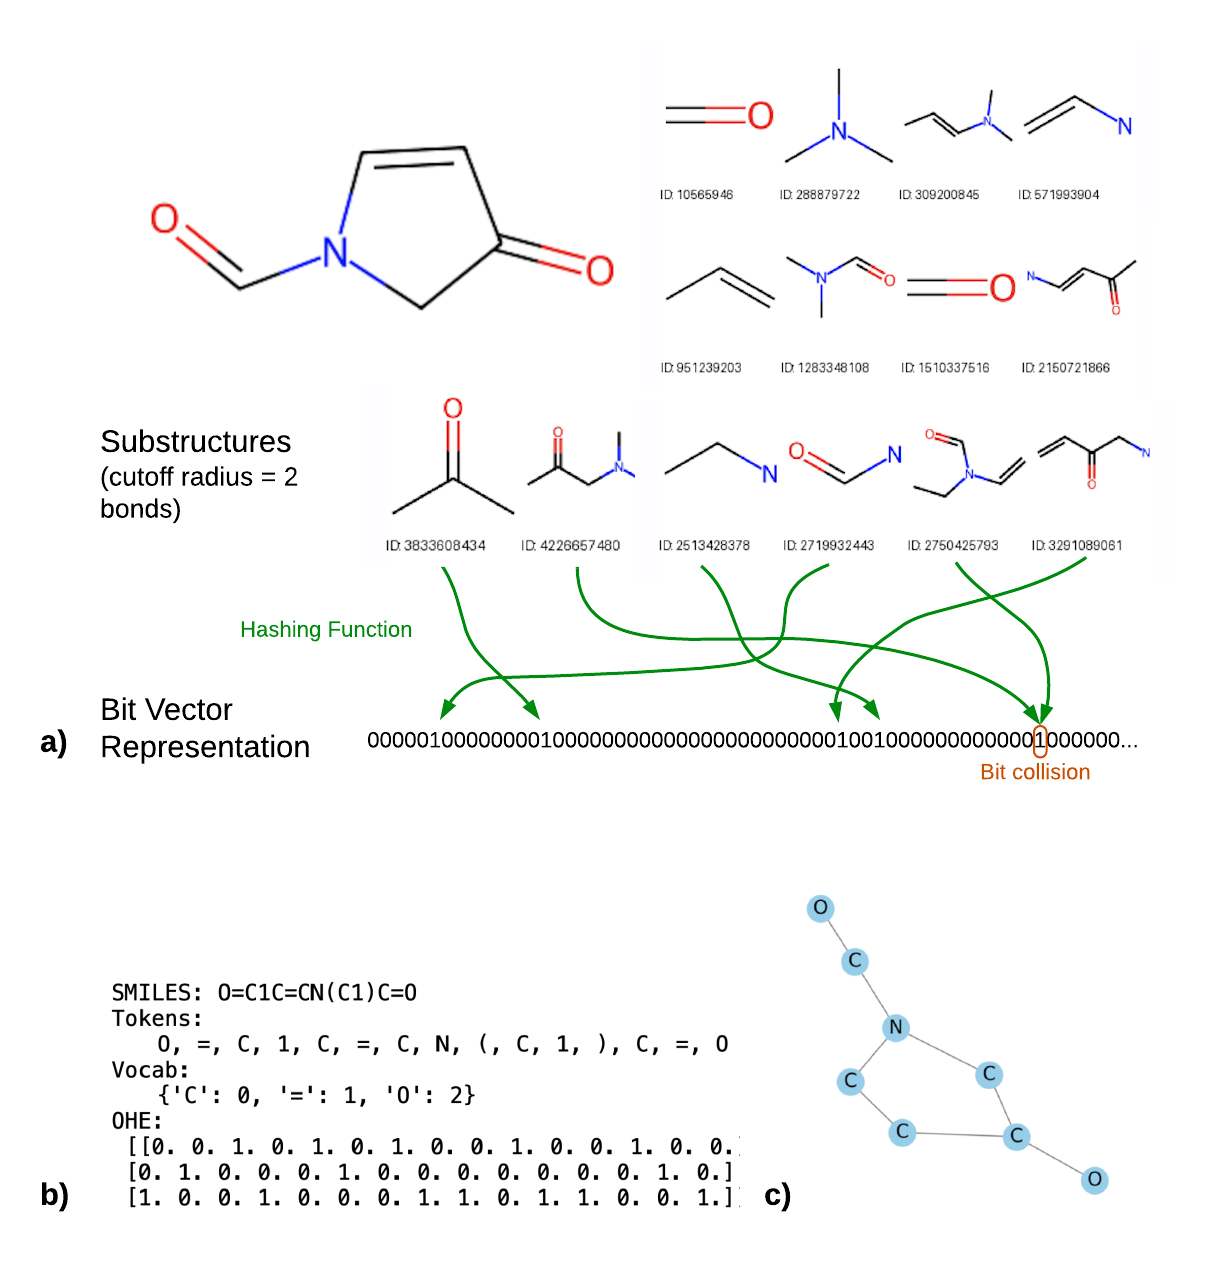
\includegraphics[width=\textwidth,height=0.72\textheight,keepaspectratio]{molecular_representations.png}
    \caption[Three representations of one molecule.]{\label{fig:molecular_representations}Three representations of the molecule \lstinline{O=C1C=CN(C1)C=O}. a) ECFP4, in which circular substructures up to a radius of two bonds are hashed (green arrows) to positions in a bit vector, and two substructures can share a position (bit collision, orange). b) Tokenization and one-hot encoding of the SMILES string. c) Molecular graph, with atoms as nodes and bonds as edges.}
\end{figure}

% [CLAUDE 2026-10-09] citation note: TeachOpenCADD2023 could not be checked (ChemRxiv 403); its one-hot notebook tokenizes per character, not into atomic branches and symbols.
One of the most common and intuitive molecular representations is the Simplified Molecular-Input Line-Entry System (SMILES) string, which consists of a sequence of ASCII characters generated by a fixed set of rules to specify a given chemical identity \citep{Weininger1988}. A common way to use SMILES strings as inputs to QSAR models is to tokenize and one-hot-encode them rather than to use the strings themselves \citep{TeachOpenCADD2023}. The strings are tokenized into atomic branches and symbols and mapped to indices of a vocabulary, and finally converted into binary vectors using one-hot encodings \citep{TeachOpenCADD2023}. This representation, referred to as one-hot-encoded SMILES, allows models to process molecular structures as bit-vector-based fingerprints or as sequences of vectors. Sequence-based models such as recurrent neural networks and transformers have proven to be particularly successful in capturing text semantics within a sequence. When applied to raw or one-hot-encoded SMILES strings, these models can effectively capture the structure of the molecule in its textual representation \citep{TeachOpenCADD2023}. 

% [CLAUDE 2026-10-09] citation note: several sentences in this paragraph are near-verbatim from Fassio2022 and Xie2020 (e.g. 'each bit accounts for the presence (1) or absence (0)...'); paraphrase or quote. 'length of 2048 bits, and active chirality flags' is not in Xie2020.
Another common representation is the molecular fingerprint, a vector containing information about the properties of the molecule in question. In a typical bit vector-based fingerprint, each bit accounts for the presence (1) or absence (0) of a given chemical feature or substructure \citep{Fassio2022}. One common fingerprint is the Molecular ACCess System (MACCS) key, a substructure key-based fingerprint that encodes predefined atom symbols and properties, as well as bond types \citep{Xie2020}. Another is the Extended Connectivity Fingerprint (ECFP), which encodes local neighborhoods around each atom and bond connectivity in molecules \citep{Xie2020}. ECFPs are typically constructed with a radius of 2, a length of 2048 bits, and active chirality flags. These existing molecular representations are well established and have been quite successful when coupled with QSAR models \citep{CortsCiriano2020, Sabando2021}. They are relatively simple, and as the bits can be mapped back to one or more substructures, they are human-interpretable, and furthermore easy-to-compute. However, they are subject to information loss due to bit collisions, which happens when two different substructures are encoded at the same bit position \citep{Fassio2022}. They are also based on a fixed procedure and are not trainable or adaptable to a particular dataset. Alternative representations that capture different structural, chemical, or physical features are able to overcome these limitations. 

Recent advances have led to the development of new molecular fingerprints. One such method is the Sort \& Slice (SNS) technique, an alternative to hash-based folding for pooling ECFP substructures \citep{sns}. Sort \& Slice begins by sorting all circular substructures in the training set according to their frequency of occurrence. It then ``slices'' away all but the $N$ most frequent substructures, which are subsequently used to generate an $N$-dimensional, bit-collision-free binary fingerprint. This approach solves the ambiguity problem of hashed fingerprints, where multiple substructures might be encoded at the same bit position, making it very interpretable \citep{sns}. Sort \& Slice fingerprints outperform ECFP of diameter four (ECFP4) with standard hash-based folding methods across various molecular property prediction tasks. These experiments consisted of different data splitting techniques, machine learning models, fingerprint diameters, fingerprint dimensions, and atomic invariants \citep{sns}. Furthermore, Sort \& Slice outperformed advanced substructure selection schemes such as filtered fingerprints and mutual information maximization \citep{sns}. 


Neural fingerprints are a category of learned  representations that overcome the fixed, hard-coded nature of traditional fingerprints. Unlike ECFP or MACCS keys, which rely on predefined hashing schemes or substructure catalogs, neural fingerprints train on molecular data to capture chemical information \citep{Jaeger2018, Chithrananda2020}. These representations are the result of deep learning architectures that have learned dense, continuous embeddings which can be used for downstream tasks. 

Mol2vec, which adapts the Word2vec algorithm from NLP to molecular substructures \citep{Jaeger2018}, is a common neural fingerprint. Mol2vec treats molecules like ``sentences'' and circular substructures derived from Morgan fingerprints like ``words''. The model learns vector embeddings for each substructure through unsupervised training, such that chemically similar substructures are mapped to nearby points in the embedding space \citep{Jaeger2018}. The embeddings of all present substructures are summed to obtain a full representation. This approach produces 300-dimensional dense vectors that avoid the sparsity and bit collisions inherent in hashed fingerprints \citep{Jaeger2018}. Mol2vec has performed strongly on various QSAR benchmarks, matching or exceeding Morgan fingerprints on solubility and bioactivity prediction tasks \citep{Jaeger2018}.

% [CLAUDE 2026-10-09] citation fix: Fabian2020 has no graph baseline.
% [CLAUDE 2026-10-09] citation fix: Chithrananda2020's default tokenizer is generic BPE; it reports selective neurons, not specialized attention heads.
% [CLAUDE 2026-10-09] citation fix: Ahmad2022 claims only 'competitive'; ChemBERTa-2 is lower than ChemBERTa on ClinTox.
Transformer-based architectures have also been applied to molecular representation learning, similarly stemming from NLP ideas. MolBERT applies a bidirectional transformer to learn molecular representations from SMILES strings through self-supervised pre-training \citep{Fabian2020}. The model has domain-relevant auxiliary adaptations, such as the prediction of calculated physicochemical properties alongside the masked token prediction, to improve the chemical fidelity of the learned embeddings \citep{Fabian2020}. MolBERT outperformed ECFP4, RDKit descriptors and the CDDD neural representation on virtual screening and QSAR benchmarks \citep{Fabian2020}. ChemBERTa is another transformer-based approach which pre-trains masked language models on SMILES data from PubChem \citep{Chithrananda2020}.  ChemBERTa uses a byte-pair-encoding tokenizer by default and compares it with a SMILES-specific tokenizer \citep{Chithrananda2020}. Attention visualization shows neurons selective for chemically relevant functional groups and aromatic rings, and others that track bracket closures in the SMILES string \citep{Chithrananda2020}. ChemBERTa-2, pre-trained on up to 77 million PubChem compounds, is competitive with existing architectures on MoleculeNet \citep{Ahmad2022}.

% [CLAUDE 2026-10-09] citation fix: Jaeger2018 presents 'pretrained once' as an advantage, not cost; Chithrananda2020 does not call them black boxes.
Neural fingerprints provide several advantages over traditional fingerprints. They produce dense continuous vectors that avoid sparseness and information loss from bit collisions \citep{Jaeger2018}. They can also be pre-trained once on large unlabeled datasets and then fine-tuned for specific downstream tasks, opening the door to transfer learning \citep{Chithrananda2020, Fabian2020}. However, pre-training them is computationally expensive, and they are less directly interpretable than fingerprints, although attention visualization offers some insight \citep{Chithrananda2020}.

% [CLAUDE 2026-10-09] citation fix: Cherkasov2014 says it is difficult to discern a clear physical-chemical interpretation for many descriptors.
Beyond fingerprints, physicochemical-descriptor vectors (PDVs) are a class of continuous-value molecular descriptors that encode structural and chemical properties of molecules \citep{Todeschini2009}. Unlike binary fingerprints or graph-based representations, PDVs aggregate atom and bond-level quantities into fixed-length feature vectors that capture a wide variety of information about a molecule and its structure \citep{Mauri2006}. PDVs typically consist of hundreds of properties including constitutional descriptors such as molecular weight, atom and bond counts, and heteroatom ratios; topological indices encoding molecular connectivity patterns; physicochemical properties such as logP (lipophilicity), molar refractivity, and topological polar surface area; and electronic descriptors derived from partial charges and polarizabilities \citep{Todeschini2009, Cherkasov2014}. The \texttt{RDKit} cheminformatics toolkit provides a comprehensive suite of more than 200 molecular descriptors that cover these categories \citep{rdkit}. Many PDV descriptors, such as logP, molecular weight and partial charges, have a direct physicochemical meaning, although many of the thousands available have no clear interpretation \citep{Cherkasov2014}. They are also less computationally expensive than some 3D methods or neural fingerprints, with many descriptors simply requiring a 2D molecular structure without conformer generation or extensive pre-training. This efficiency makes PDVs particularly appropriate for high-throughput applications. Descriptors based on 3D structure can also be used \citep{Mauri2006}.

% [CLAUDE 2026-10-09] citation fix: Mauri2006 (DRAGON software) does not make this comparison; the sentence is our own reasoning.
However, PDVs have limitations. The dimensionality of PDV feature spaces can lead to problems with multicollinearity \citep{Todeschini2009}. This can be mitigated by feature selection or dimensionality reduction techniques \citep{Cherkasov2014}. Additionally, PDVs encode molecular properties as aggregated global features, which may not capture fine-grained structural details such as specific substructure arrangements or local chemical environments, information important for particular endpoints.

% [CLAUDE 2026-10-09] citation fix: matched to Zhichun2023 Table 1; if the earlier lists were our own features, state them without this citation.
One of the more intuitive representations is the molecular graph. These graphs can be categorized into 2D and 3D graphs. 2D graphs rely on adjacency matrices that encode topological atom- and bond-level features but leave out geometric properties such as bond angles or torsion, meaning they may fail to capture stereochemistry. 3D graphs incorporate these spatial features, but are often limited by remaining in a single conformation \citep{Zhichun2023}. A standard molecular graph is constructed such that each molecule is represented as $G = (V,E)$ with node features $\mathbf{x}_i$ and edge features $\mathbf{e}_{ij}$. In one common featurization, nodes encode atom type, chirality, hybridization and aromaticity, and edges encode bond type, ring membership, direction and stereochemistry \citep{Zhichun2023}. 

% [CLAUDE 2026-10-09] citation fix: 'standard distance compatibility molecular graph' is not in David2020; Hnig2022 reviews superposition methods (full text not checked).
% [CLAUDE 2026-10-09] citation fix: voxel sparsity is a property of 3D grids, not graphs (Kuzminykh2018).
In the standard molecular graph, atoms are mapped to nodes and bonds to edges \citep{David2020}. These molecular graphs are typically 2D objects that represent 3D information such as atomic coordinates, bond angles, chirality, etc. \citep{David2020}. However, there are alternative molecular graph representations such as graphs with quantum 3D embeddings, weight alignment graphs, association graphs containing pairs of molecules, and geometric interaction graph neural networks that incorporate 3D structures and physical interactions \citep{Hnig2022, yan2023, Yang2023GIGN}. \citet{Du2022} developed hybrid 2D and 3D graphs, combining 3D data, guaranteeing precision and completeness by providing unabridged information, and 2D data, providing chemical intuitions for guidance, in a zipper-like arrangement. Voxel-based 3D representations, in which each atom occupies one grid cell, are too sparse for convolutional networks to perform well; \citet{Kuzminykh2018} instead spread each atom over nearby voxels with a wave transform.
      
% [CLAUDE 2026-10-09] citation fix: ross2022 (MoLFormer) is a SMILES transformer, not a GNN.
These graph representations do not highlight specific substructures or specific arrangements of atoms and bonds within each molecule. The substructures contain functional groups that are related to a range of chemical properties and are potentially involved in downstream tasks related to the function of molecules. \citet{Bouritsas2023} developed graph substructure networks, a topologically aware message passing scheme based on substructure encoding. The method involves encoding structural roles based on the appearance of specific substructures and using them in message passing updates. Since message-passing graph neural networks (GNNs) are at most as powerful as the Weisfeiler--Lehman test, they cannot isolate sufficient features from the graph structure \citep{Bouritsas2023}. Graph substructure networks, on the other hand, capture these substructure-related features. Encoders pretrained on unlabeled molecules, whether graph-based \citep{kishimoto2023} or transformers on SMILES \citep{ross2022}, can also produce embeddings that capture structural features. 

\section{Models for molecular property prediction}
% [notes moved to thesis_notes_moved.md]

There are a wide variety of model architectures that can be used for QSAR modeling. Starting off with simpler and more explainable models, we have tree-based methods. Decision trees are non-parametric supervised learning algorithms that perform recursive binary partitioning of the feature space \citep{Breiman1984}. A decision tree builds a predictive model by learning a series of if-then rules that recursively split the data based on given feature values, creating a tree  where internal nodes represent decision rules, branches represent the results of those decisions, and leaf nodes contain predicted values or class labels \citep{Breiman1984}. Each recursive split is chosen to maximize  homogeneity within the resulting partitions. For classification, Gini impurity is commonly used and for regression, mean squared error reduction \citep{Breiman1984}.

There are several properties that make decision trees a good foundation for QSAR modeling. First, they handle non-linear relationships between molecular descriptors and target properties without requiring explicit feature engineering or transformation \citep{Breiman1984}. They also do not make assumptions about the underlying distribution of the data, making them robust to violations of parametric assumptions that can limit linear regression or other classical methods \citep{Svetnik2003}. 

Decision trees handle data in a ``contributory'' rather than ``consensus'' manner. In consensus methods such as linear regression or neural networks, every data point influences the prediction at every other point in the feature space. Tree-based methods make predictions based on the subset of training samples that fall into the same leaf node as the test point \citep{Breiman1984}. This mechanism essentially quarantines outliers in their respective leaf nodes, limiting their impact on predictions for samples in other regions or chemical domains. 

% [CLAUDE 2026-10-09] citation fix: tree instability is from Breiman 1996 (bagging), not the Random Forests paper.
% [CLAUDE 2026-10-09] citation fix: 'preventing systematic biases from propagating' is not in Breiman2001.
Individual decision trees tend to have high variance and often overfit, particularly at large depths \citep{Breiman1984}. Small modifications made to the training data can result in large differences in the structure of the tree, resulting in unstable predictions \citep{Breiman1996}. Ensemble methods are used to counteract this instability, aggregating predictions from many trees. Random forests (RFs) aggregate predictions from trees trained on bootstrap samples of data with random subsets of features at each split \citep{Breiman2001}. Bootstrapping ensures that each tree is trained on a slightly different subset of data, which effectively reduces the influence of any individual sample \citep{Breiman2001}. This is especially beneficial with noisy samples. The selection of random features at every node decorrelates the trees, which lowers the generalization error of the ensemble \citep{Breiman2001}. The aggregation of trees further prevents overfitting to noise by smoothing out prediction errors from individual noisy labels. 

Neural networks (NNs), a very popular family of models, can also be used for QSAR, although with mixed results. An NN is a system of interconnected nodes which learn by passing information through its layers. There are weights and biases attached to the nodes and various other parameters which the model optimizes to minimize the difference between the predicted output and the actual target value. During training, the network parameters are updated using backpropagation, in which gradients of the loss function with respect to each weight are propagated backward through the network \citep{Rumelhart1986}. The structure of these networks and the hyperparameters used depend on the type of NN. In QSAR, one of the most commonly used architectures is the multilayer perceptron (MLP), a NN containing fully-connected layers with non-linear activation functions which transforms molecular feature vectors (i.e., fingerprints, descriptors) into a property or activity prediction \citep{Ma2015}.

% [CLAUDE 2026-10-09] citation fix: wu2018 (MoleculeNet) does not recommend 2-3 layers of 128-512 units; it lists the hyperparameters it searched. Citation and the specific numbers removed; if these are our own settings, say so.
A typical MLP for molecular property prediction has a few fully connected hidden layers with rectified linear unit (ReLU) activations and dropout regularization to prevent overfitting. Training is performed using backpropagation with gradient descent optimizers such as Adam, to minimize a loss function (mean squared error for regression, cross-entropy for classification) on batches of training data. 

% [CLAUDE 2026-10-09] citation fix: Koutsoukas2017 finds the reverse of 'NNs are often outperformed' (tuned DNNs outperform NB, kNN, RF, SVM); Baskin2008 is a review making no such comparison; neither says MLPs use 3D structure. Sentence on small datasets/3D removed: find a source if wanted.
However, NN performance on QSAR-related tasks has been very mixed. NNs have a long history in QSAR \citep{Baskin2008}, and tuned deep networks have outperformed shallow methods such as random forests and support vector machines across diverse activity classes \citep{Koutsoukas2017}. Their complexity and use of gradients make them prone to label memorization \citep{Zhang2017}, which in the context of noise is problematic, as it means that models may memorize the noise themselves. Although models that are memorizing labels may initially appear to have strong predictive performance, they cannot generalize to out-of-distribution samples properly and often provide inaccurate uncertainty estimates. Various approaches have been proposed to improve neural network robustness to label noise, including noise-robust loss functions \citep{Song2022}, confident learning to identify mislabeled examples \citep{Northcutt2021}, and regularization techniques such as mixup \citep{Zhang2018mixup} or label smoothing \citep{Szegedy2015}. 

% [CLAUDE 2026-10-09] citation fix: the GCN is Kipf & Welling 2017; TeachOpenCADD and Xu2019 are later.
% [CLAUDE 2026-10-09] citation fix: TeachOpenCADD does not say GINs suit activity cliffs.
All the models up to this point have assumed a vector-based input. Molecular graphs, on the other hand, require different types of predictive modeling. Two standard ML methods on molecular graphs include Graph Convolutional Networks (GCNs) and Graph Isomorphism Networks (GINs). GCNs apply the concept of convolution to graph-structured data. Instead of operating on grid-based data, such as images, GCNs aggregate information from neighbors of a node to update its representation \citep{Kipf2017}. In contrast, GINs address the limitations in GCNs’ ability to differentiate between non-isomorphic graphs. Unlike GCNs, which normalize and weight the sum of neighboring node features, GINs use a simple sum followed by a trainable MLP, giving the model flexibility to learn complex transformations of node features. The GIN model’s design is informed by the Weisfeiler--Lehman test for graph isomorphism, enabling it to distinguish between molecular graphs that are structurally similar but differ in subtle ways \citep{TeachOpenCADD2023, Xu2019}. GIN features have been competitive with or better than fingerprints and descriptors at classifying pairs of molecules as activity cliffs (ACs; Section~\ref{sec:mol_similarity}), where small variations in molecular structure can lead to significant changes in chemical or biological activity \citep{Dablander2023}. Descriptor-based models still predicted the potency of cliff molecules better than deep learning methods \citep{vanTilborg2022}. 


\subsection{Tree ensembles}

Gradient boosting methods such as eXtreme Gradient Boosting (XGBoost) sequentially fit trees to the residuals of previous iterations, progressively reducing the prediction error \citep{Chen2016, Mustapha2016, Tian2022}. We used a handful of gradient-boosted tree ensembles in this thesis including Light Gradient-Boosting Machine (LightGBM) \citep{ke2017lightgbm}, and Natural Gradient Boosting (NGBoost) \citep{Duan2020}.

\subsection{Support vector machines}
% [notes moved to thesis_notes_moved.md]

% CODE INPUT
% TODO: review, needs manual review
% [CLAUDE 2026-10-09] citation fix: the epsilon-tube trade-off is the SVR formulation (Smola2004); Cortes1995 is the classification SVM.
Support vector regression fits a function that is as flat as possible while keeping training errors small \citep{Vapnik1995, Smola2004}. It uses the $\epsilon$-insensitive loss, under which errors smaller than $\epsilon$ cost nothing and larger errors cost their size minus $\epsilon$. A constant $C$ trades flatness against tolerance of large errors \citep{Cortes1995, Smola2004}. The features enter the model only through the kernel. With the radial basis function (RBF) kernel, the kernel is a function of the Euclidean distance, so every feature enters every distance. In Chapter~\ref{chap:robustness} the continuous representations are standardized and the binary fingerprints are used as built. Three properties of the method suggest robustness to label noise. Errors inside the $\epsilon$ tube change nothing, the loss outside the tube grows linearly rather than quadratically, and the weight of each molecule is capped at $C$ \citep{Smola2004}. Under simulated experimental error, the RBF-kernel SVM degraded smoothly and linearly \citep{Cortes2015}, and Chapter~\ref{chap:robustness} reports how it holds up under each of our noise conditions. Its main limitation is computational cost, because training operates on a kernel matrix that grows with the square of the number of training molecules \citep{Chang2011}.


\subsection{Gaussian processes}

We employed Gaussian process (GP) models using the \texttt{Gauche} framework \citep{gauche}, which is optimized for cheminformatics tasks. Standardized kernels for GPs are not optimized for the chemical landscape. GAUCHE defines such kernels for strings, fingerprints, and graphs that operate on a range of widely used molecular representations \citep{gauche}. We used the Tanimoto kernel \citep{Ralaivola2005, moss2020}, which is defined for binary vectors $\mathbf{x}, \mathbf{x}' \in \{0, 1\}^d$ for $d \geq 1$ as:

\begin{equation}
k_{\text{Tanimoto}}(\mathbf{x}, \mathbf{x}') := \sigma_f^2 \cdot \frac{\langle \mathbf{x}, \mathbf{x}' \rangle}{\|\mathbf{x}\|^2 + \|\mathbf{x}'\|^2 - \langle \mathbf{x}, \mathbf{x}' \rangle},
\label{eq:tanimoto_kernel}
\end{equation}

where $\|\cdot\|$ represents the Euclidean norm \citep{gauche}. 

The RBF kernel is defined for
$\mathbf{x}, \mathbf{x}' \in \mathbb{R}^d$ as:

\begin{equation}
k_{\text{RBF}}(\mathbf{x}, \mathbf{x}') := \sigma_f^2 \cdot \exp\left(-\frac{\|\mathbf{x} - \mathbf{x}'\|^2}{2\ell^2}\right),
\end{equation}

where $\ell$ is the lengthscale and $\sigma_f^2$ the signal variance, which scales both kernels.


\subsection{Bayesian neural networks}

Standard feed-forward networks are deterministic; however, they can be transformed into probabilistic models (Figure~\ref{fig:bayesian_transformation}).

\begin{figure}[!htbp]
    \centering
    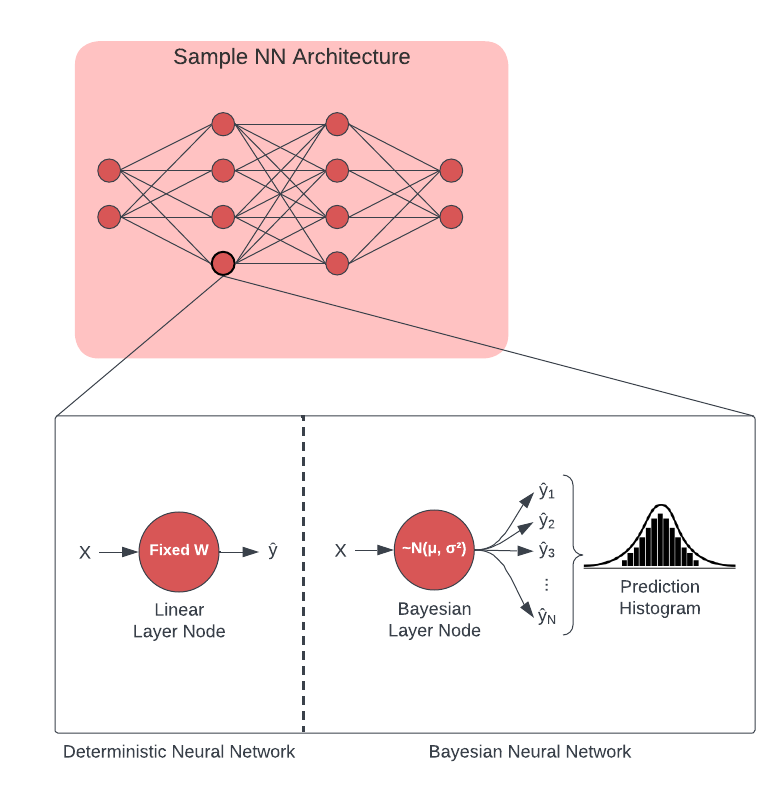
\includegraphics[width=0.85\textwidth,height=0.72\textheight,keepaspectratio]{bayesian_transformation.png}
    \caption[Nodes of a deterministic and a Bayesian neural network.]{One node of a deterministic and of a Bayesian neural network. The deterministic node (bottom left) applies a fixed weight $W$ and returns one prediction $\hat{y}$. The Bayesian node (bottom right) draws its weight from $\mathcal{N}(\mu, \sigma^2)$, so repeated predictions $\hat{y}_1, \dots, \hat{y}_N$ form a histogram.}
    \label{fig:bayesian_transformation}
\end{figure}

% [CLAUDE 2026-10-09] citation fix: Hanser2023 is a federated-learning review, not about uncertainty estimation.
Unlike standard deterministic ML methods, Bayesian methods model distributions over predictions using Bayes' rule, allowing for the quantification of uncertainty within parameters and labels. Bayesian methods treat the model parameters as random variables with distributions. Uncertainty can also be estimated from other non-deterministic methods, including deep ensembles \citep{lakshminarayanan2017} and bootstrap modeling \citep{palmer2022}.


\section{Molecular similarity and activity cliffs}\label{sec:mol_similarity}

% TODO: review, needs manual review
Much of cheminformatics rests on the similar property principle, which states that structurally similar molecules tend to have similar properties \citep{Johnson1990, vanTilborg2022}.
One of its clearest applications is nearest-neighbor prediction, which appears across cheminformatics workflows and, in this thesis, in the kernels used by GPs and at the basis of many noise identification algorithms.

% TODO: review, needs manual review
The difficulty with this principle is that similarity is defined only relative to a similarity measure, which is fixed by the choice of representation and
coefficient \citep{Maggiora2014}. There is no standard definition of similarity between molecules, especially when different molecular embeddings are handled in a computational setting. Two molecules that are near-identical under a substructure fingerprint may be far apart under a PDV, and \citet{Maggiora2014} caution that quantified similarity can be over-interpreted in this way.

% CODE INPUT: formula added so that Chapter 4's argument about distances has its starting point here
The most common measure for binary fingerprints is the Tanimoto coefficient \citep{Bajusz2015}. For two molecules with fingerprints $\mathbf{x}, \mathbf{x}' \in \{0,1\}^d$,
\begin{equation}
T(\mathbf{x}, \mathbf{x}') = \frac{\sum_{j=1}^{d} x_j x'_j}{\sum_{j=1}^{d} x_j + \sum_{j=1}^{d} x'_j - \sum_{j=1}^{d} x_j x'_j},
\label{eq:tanimoto}
\end{equation}
which is the number of bits set in both molecules divided by the number of bits set in either. Continuous representations are instead compared with a distance, most often the Euclidean distance $\sqrt{\sum_{j=1}^{d}(x_j - x'_j)^2}$. Both measures are sums over the features, and neither weighs a feature by its relation to the property. In the Tanimoto coefficient, a bit that is off in both molecules contributes nothing, whereas every bit that is set in either molecule counts. In the Euclidean distance, every feature that differs between the two molecules counts. Chapter~\ref{chap:flaws} returns to this point (Equation~\ref{eq:distance_split}).

% [CLAUDE 2026-10-09] citation fix: Bajusz2015 does not compare strong and weak representations; that part is now marked as our inference.
Distance-based reasoning relies on the assumption that the data embeddings contain quality information. When the labels are corrupted or the important features are scarce, similarity scores over-rely on compounding false or useless information, and the assumption that similar molecules have similar properties breaks down. \citet{Bajusz2015} found that the Tanimoto, Dice and Cosine coefficients and the Soergel distance rank molecules almost identically on binary fingerprints. We take this to mean that changing the formula cannot compensate for a weak representation.
This problem is further complicated by activity cliffs (defined below). These molecules, which potentially contain the most important information for model prediction, can be confused with noise. Another barrier to distance-based reasoning is persistent noise across labels. The task of trying to determine if a molecule's value matches that of its neighbors becomes a lot harder when all of the neighbors have some form of noise as well.

There are many downstream tasks which rely on the concept of similarity. The second half of this thesis relies on many such tasks, and as such focuses on identifying representations that agree with this principle. 


% TODO: review, needs manual review
The sharpest failure of the similar property principle is the activity cliff, a pair of structurally similar molecules with a large difference in potency that is produced by a small
chemical change \citep{Maggiora2006, Stumpfe2012}. Activity cliffs inherit the measure dependence of the principle they violate, and there is no widely accepted definition of one
\citep{vanTilborg2022}. The MoleculeACE benchmark \citep{vanTilborg2022} makes this choice explicit. A pair is considered highly similar if its similarity exceeds 90\% under at least one of
three measures, namely the Tanimoto coefficient on ECFPs, the Tanimoto coefficient on scaffold fingerprints and a scaled Levenshtein distance on SMILES strings. Such a pair forms a cliff if
the two molecules also differ tenfold or more in $K_i$ or EC$_{50}$ \citep{vanTilborg2022}. This soft consensus over three measures is used because each measure captures only part of the
underlying chemistry. Across the thirty MoleculeACE targets, cliff compounds account for between 7\% and 52\% of a dataset \citep{vanTilborg2022}.

% TODO: review, needs manual review
% [CLAUDE 2026-10-09] citation fix: the convergence of nearest and furthest distances is Beyer1999; Aggarwal2001 shows it depends on the distance metric.
Dimensionality itself poses a further difficulty. \citet{Beyer1999} show that as the number of dimensions grows, the distances to the nearest and to the furthest
point become increasingly similar, so that pairwise distances become progressively less discriminative. Molecular representations are routinely high-dimensional and sparse, and when a
large proportion of their dimensions carry no information relevant to the property being modeled, distances computed over them are dominated by those uninformative dimensions.


\section{Noise in molecular data}
% [notes moved to thesis_notes_moved.md]

Real-world cheminformatics datasets contain label noise arising from multiple sources across the drug discovery pipeline. Although noise is often modeled as being random, or drawn from a Gaussian distribution, other varieties of noise must be considered when working with experimental data. To properly model experimental noise, we must first understand where the noise is coming from.

% moved here from the start of the Models section (2026-09-30)
% [CLAUDE 2026-10-09] citation fix: Kolmar2021 names GPs and conformal prediction, not BNNs.
One key issue with QSAR models is the standard ML assumption that labels represent true values, as most chemical datasets lack sufficient replications to provide a robust statistical representation of the underlying distributions \citep{Kolmar2021}. A single measurement, or even multiple measurements for a given label, will not guarantee that this label accurately reflects the population mean \citep{Kolmar2021}. Most ML models rely on the assumption that the training data is, in fact, an accurate reflection of the population. Therefore, they treat these potentially noisy labels as discrete quantities rather than distributions, which opens the door to overfitting to noise. However, Bayesian methods such as Gaussian processes (GPs), and conformal prediction, do not make this assumption \citep{Kolmar2021}.

% [CLAUDE 2026-10-09] citation fix: Kruger2012's Laplace fit is to differences between orthologs and paralogs; repeat-assay differences are only said to resemble them.
% [CLAUDE 2026-10-09] citation fix: Kalliokoski2013: 9, 10 and 8 of 10 inspected pairs; the paper says 'in most cases'.
Studies involving noise, and specifically the quantification of noise robustness, typically approach label noise by adding independent, zero-mean, Gaussian error to the labels. However, there's evidence to suggest that noise from experimental assays takes on different forms. \citet{Kruger2012} rejected normality of the differences in binding affinity between orthologous targets by Anderson-Darling test, found them approximately Laplace, and found that differences between assays of the same ligand and target closely resemble them. \citet{Kalliokoski2013} examined the widest disagreements among 16,844 pairs of repeat pIC$_{50}$ measurements and found that in most cases, the wide gap between repeat values was due to annotation error rather than to an imprecise assay. 

% [CLAUDE 2026-10-09] citation fix: Heid2023 injected the nitrogen-dependent noise on purpose; it is not an observed measurement effect.
Although numerous studies have explored the effects of noise on ML algorithms for molecular property prediction, comparisons between different molecular representations remain limited. \citet{Kolmar2021} examined the predictive limits of QSAR in the presence of noise, showing that by learning the underlying trends rather than fitting to noise, the models can achieve predictions more accurate than those of their training data. They assumed experimental noise could be modeled as Gaussian-distributed, using the Central Limit Theorem to argue that aggregated experimental measurements from multiple independent error sources exhibit a Gaussian distribution. However, \citet{Heid2023} distinguish random noise, which affects all molecules alike, from systematic noise that differs between regions of chemical space. Using synthetic noise applied only to nitrogen-containing molecules, they showed that mean-variance estimation can detect it.

% [CLAUDE 2026-10-09] citation fix: Bentz2013's 62% is for the cell-line laboratories only (11 + 6 + 4), digoxin efflux ratio, Table 7.
Beyond just the distribution, the assumptions of independence and zero mean may fail as well. \citet{Bentz2013} examined P-glycoprotein transport measurements from 23 laboratories and found that, among the laboratories using cell lines, 62\% of the variance in log digoxin efflux ratio was due to differences between laboratories. When you pool data from different sources, each source has the potential to carry a shared offset. These sources usually contain families of related compounds, breaking the independence assumption. The zero-mean assumption is not assured either, especially when true values fall above or below an assay's detection limit, called censoring. \citet{Svensson2025} count censored labels in 15 industrial assays, of which 13 carry censored labels and eight sit between a quarter and two thirds censored. Chapter~\ref{chap:robustness} tests noise conditions that vary the distribution, the correlation, and the bias of injected error separately, at a matched quantity of noise for every condition except censoring.

% Original six paragraphs on noise sources, now Table tab:noise_sources:
% Assay-related variability represents a primary source of label noise in bioactivity data. High-throughput screening assays are often laden with errors from physical phenomena such as edge effects, where compounds in wells exhibit different activities at plate boundaries due to evaporation or temperature gradients \citep{Macarron2011}. Other examples include compound carryover between wells, incomplete liquid transfers, and air bubbles  \citep{Inglese2006}.  Detection reagents or unstable compounds can degrade over time, which leads to drift within a single plate run. This turns into heteroscedastic noise correlated with plate position or read time \citep{Brideau2003}.
% 
% Instrument calibration and detection limits can impact measurement accuracy. Spectrophotometric assays near detection limits exhibit higher relative error, such that signal-to-noise ratios degrade for weak binders \citep{Zhang1999}. Fluorescence quenching by test compounds introduces a systematic bia in fluorescence-based assays, resulting in false negatives for potent inhibitors that accidentally get absorbed at emission wavelengths \citep{Simeonov2008}. Radiometric assays require background subtraction and decay corrections that accumulate error, particularly for low-activity compounds where the signal barely exceeds background \citep{Zhang1999}.
% 
% Another source of noise is biological variability. Even minor variations in cell culture conditions such as seeding density, plating efficiency, growth rate, and cell cycle distribution have the potential to affect downstream tasks such as cell metabolism and drug responsiveness. Even serum properties may introduce variability \citep{Hatzis2014}. The speed of cell culture passages is even found to be a significant factor in behavior \citep{Postnikova2018}. 
% 
% Data aggregation across multiple sources compounds these individual error sources. Common databases like ChEMBL, BindingDB, and PubChem aggregate measurements from hundreds of laboratories using a diverse set of protocols, compound purities, and quality control standards \citep{Gaulton2017, Gilson2016}. The $K_i$ or IC$_{50}$ values from the same compound-target pair with between 10 and 20 reported values, often end up spanning two orders of magnitude apart, making it challenging to identify the underlying ground truth \citep{Kramer2012}. All the sources of error mentioned above regarding inconsistent experimental protocols cannot be distinguished easily from the genuine underlying value without extensive, and often unrealistic amounts of metadata \citep{Fourches2016}.
% 
% 
% Federated datasets, a method of data aggregation centered around privacy protection, presents a particularly challenging situation for noise. In pharmaceutical research and beyond, companies often want to merge collective information without exposing proprietary data to competitors. One example of such platforms is Lhasa Limited's federated learning platform Effiris. Teacher models are first trained separately on confidental data, and then used to label a shared public chemical data set. Those results are consolidated into a federated student model \citep{Bassani2023}. While this is an effective approach of protecting intellectual property, it introduces additional label noise through the prediction errors of all the teacher models. There also exists aleatoric uncertainty from the underlying experimental measurements, many of which likely come from differing protocols, resulting in compounding label noise. 
% 
% Beyond the experimental setups, annotation errors in the data itself can arise from mis-registered structures, incorrect stereochemistry assignments, and salt form ambiguity \citep{Williams2017}. Public databases are estimated to contain 1-5\% structure errors from incorrect SMILES parsing, tautomer misassignment, or manual transcription mistakes during data entry \citep{Young2008}. Ambiguous protonation states and counterions create representation-level noise where chemically distinct samples are classified as the same \citep{Bento2020}.

Label noise enters bioactivity data at every step from the assay plate to the database. Table~\ref{tab:noise_sources} lists these sources, with examples of each and the kind of error each tends to produce. The kind of error describes how the error is distributed across molecules, which is the property that the noise conditions in Section~\ref{sec:noise_injection} vary.
\begin{table}[htbp]
\centering
\small
\begin{adjustbox}{max width=\textwidth,max totalheight=0.78\textheight}
\begin{tabular}{@{}P{0.16\linewidth}P{0.46\linewidth}P{0.30\linewidth}@{}}
\toprule
\textbf{Source} & \textbf{Example} & \textbf{Kind of Error} \\
\midrule
% [CLAUDE 2026-10-09] citation fix: Macarron2011 does not discuss edge effects; Inglese2006 supports carryover only; 'air bubbles' had no source.
Assay & Edge, row and column effects from evaporation or temperature gradients, and errors in liquid handling \citep{Makarenkov2007}; carryover between wells \citep{Inglese2006}; reagents or compounds degrading during a run \citep{Brideau2003} & Error that varies with plate position or read time \\
% [CLAUDE 2026-10-09] citation fix: Simeonov2008 measured compound autofluorescence, not quenching.
Instrument & Higher relative error near a detection limit \citep{Zhang1999}; autofluorescence of the test compound \citep{Simeonov2008}; background subtraction in radiometric assays \citep{Zhang1999} & Larger error for weak binders; a systematic bias; labels clipped at the limit \\
% [CLAUDE 2026-10-09] citation fix: Postnikova2018 studies passage number.
Biology & Seeding density, growth rate, cell cycle and serum properties \citep{Hatzis2014}; cell passage number \citep{Postnikova2018} & Variation between repeats of the same experiment \\
% [CLAUDE 2026-10-09] citation fix: Kramer2012 is Ki only; 'two orders of magnitude' is not in its abstract.
Aggregation across sources & ChEMBL, BindingDB and PubChem pool hundreds of laboratories \citep{Gaulton2017, Gilson2016}; independent $K_i$ measurements of one compound--target pair differing by 0.44 log units on average \citep{Kramer2012} & An offset shared by each laboratory or source, hard to separate from the true value without metadata \citep{Fourches2016} \\
Federated learning & Teacher models label a shared public set, and a student model learns from those labels \citep{Bassani2023} & The teachers' prediction errors on top of the measurement error \\
% [CLAUDE 2026-10-09] citation fix: Williams2017 (CompTox Dashboard) does not report these errors; Young2008's figure is 0.1-3.4%, as quoted by Fourches2010.
Annotation & Mis-registered structures, wrong stereochemistry and salt forms \citep{Fourches2010}; 0.1--3.4\% of structures incorrect, depending on the database \citep{Young2008}; ambiguous protonation states and counterions \citep{Bento2020} & A label attached to the wrong molecule; distinct molecules merged \\
\bottomrule
\end{tabular}
\end{adjustbox}
\caption[Sources of label noise in bioactivity data.]{Sources of label noise in bioactivity data, with reported examples and the kind of error each source produces.}
\label{tab:noise_sources}
\end{table}

% CODE INPUT: first person changed to "we"
% [CLAUDE 2026-10-09] citation fix: Heid2023 does not claim real noise is non-i.i.d. and asymmetric (it found no difference between error distributions); the parts are now cited to the papers that support them.
These noise sources can interact with each other and present in more ways than a simple Gaussian. Real noise can be heteroscedastic, larger in some regions of chemical space than others \citep{Heid2023}, shared within a laboratory \citep{Bentz2013}, and non-normal \citep{Kruger2012}. We wanted to address this complexity in our research by examining a variety of ways of both modeling and adding noise to datasets.

% [CLAUDE 2026-10-09] citation fix: Ullah2024 appends noise predictors/observations with zero response; it never adds noise to labels.
Although the general assumption in much of the noise analysis and mitigation literature is that noise, specifically label noise, will have a negative effect on the model, this is not necessarily the case. There are multiple instances of using noise as a method of regularization. In linear regression, appending observations of pure noise shrinks the coefficient estimates, an implicit regularization, although not an optimal one \citep{Ullah2024}. Furthermore, adding artificial noise drawn from a Gaussian distribution to the activation layers of a neural network is considered another form of regularization \citep{Camuto2021}. These studies indicate that the presence of noise may act as a form of regularization in some contexts. It is important to address this potential of regularization from label noise in QSAR and quantitative structure--property relationship (QSPR) models.

\subsection{Artificial noise injection}\label{sec:noise_injection}
% [notes moved to thesis_notes_moved.md]

Our objective is to evaluate the robustness of QSAR models against label noise. To do so, we ``inject'' artificial noise into the labels during training while validation and test data remain free of noise. Validation labels are given noise of the same type and quantity as the training labels, drawn independently. This artificial noise simulates real-world experimental noise. The clean target label $y_i$ is replaced by a noisy label $\tilde{y}_i = y_i + \epsilon_i$, where $\epsilon_i$ is the artificial noise injected at the index $i$, the value of which is determined by a specified noise strategy. As we increased the quantity of noise, we measured how much predictive performance fell. 

% Original paragraph listing the seven conditions, now Table tab:noise_conditions:
% We explored seven methodologies of adding noise, referred to as noise conditions (Figure~\ref{fig:noise_conditions}). Three vary the shape of the distribution from which the error is drawn. These shapes include Gaussian, Student-$t$ with $\nu = 5$, and Laplace distributions. Two conditions concentrate error on specific subset of molecules; outlier isolates a random tenth of them and grouped-wider concentrates on Bemis--Murcko scaffold families. Group shifted also applies noise to scaffolds, but instead gives each scaffold its own offset rather than a wider error. The seventh, censoring, sets a limit such that every label extends past that limit is reassigned to the limit itself. 
We explored seven ways of adding noise, which we refer to as noise conditions and which are illustrated in Figure~\ref{fig:noise_conditions} and summarized in Table~\ref{tab:noise_conditions}. Three conditions vary the shape of the distribution from which the error is drawn, and three concentrate the error on some molecules or share it within Bemis--Murcko scaffold families. The seventh condition, censoring, clips labels at a limit.

\begin{figure}[!htbp]
\centering
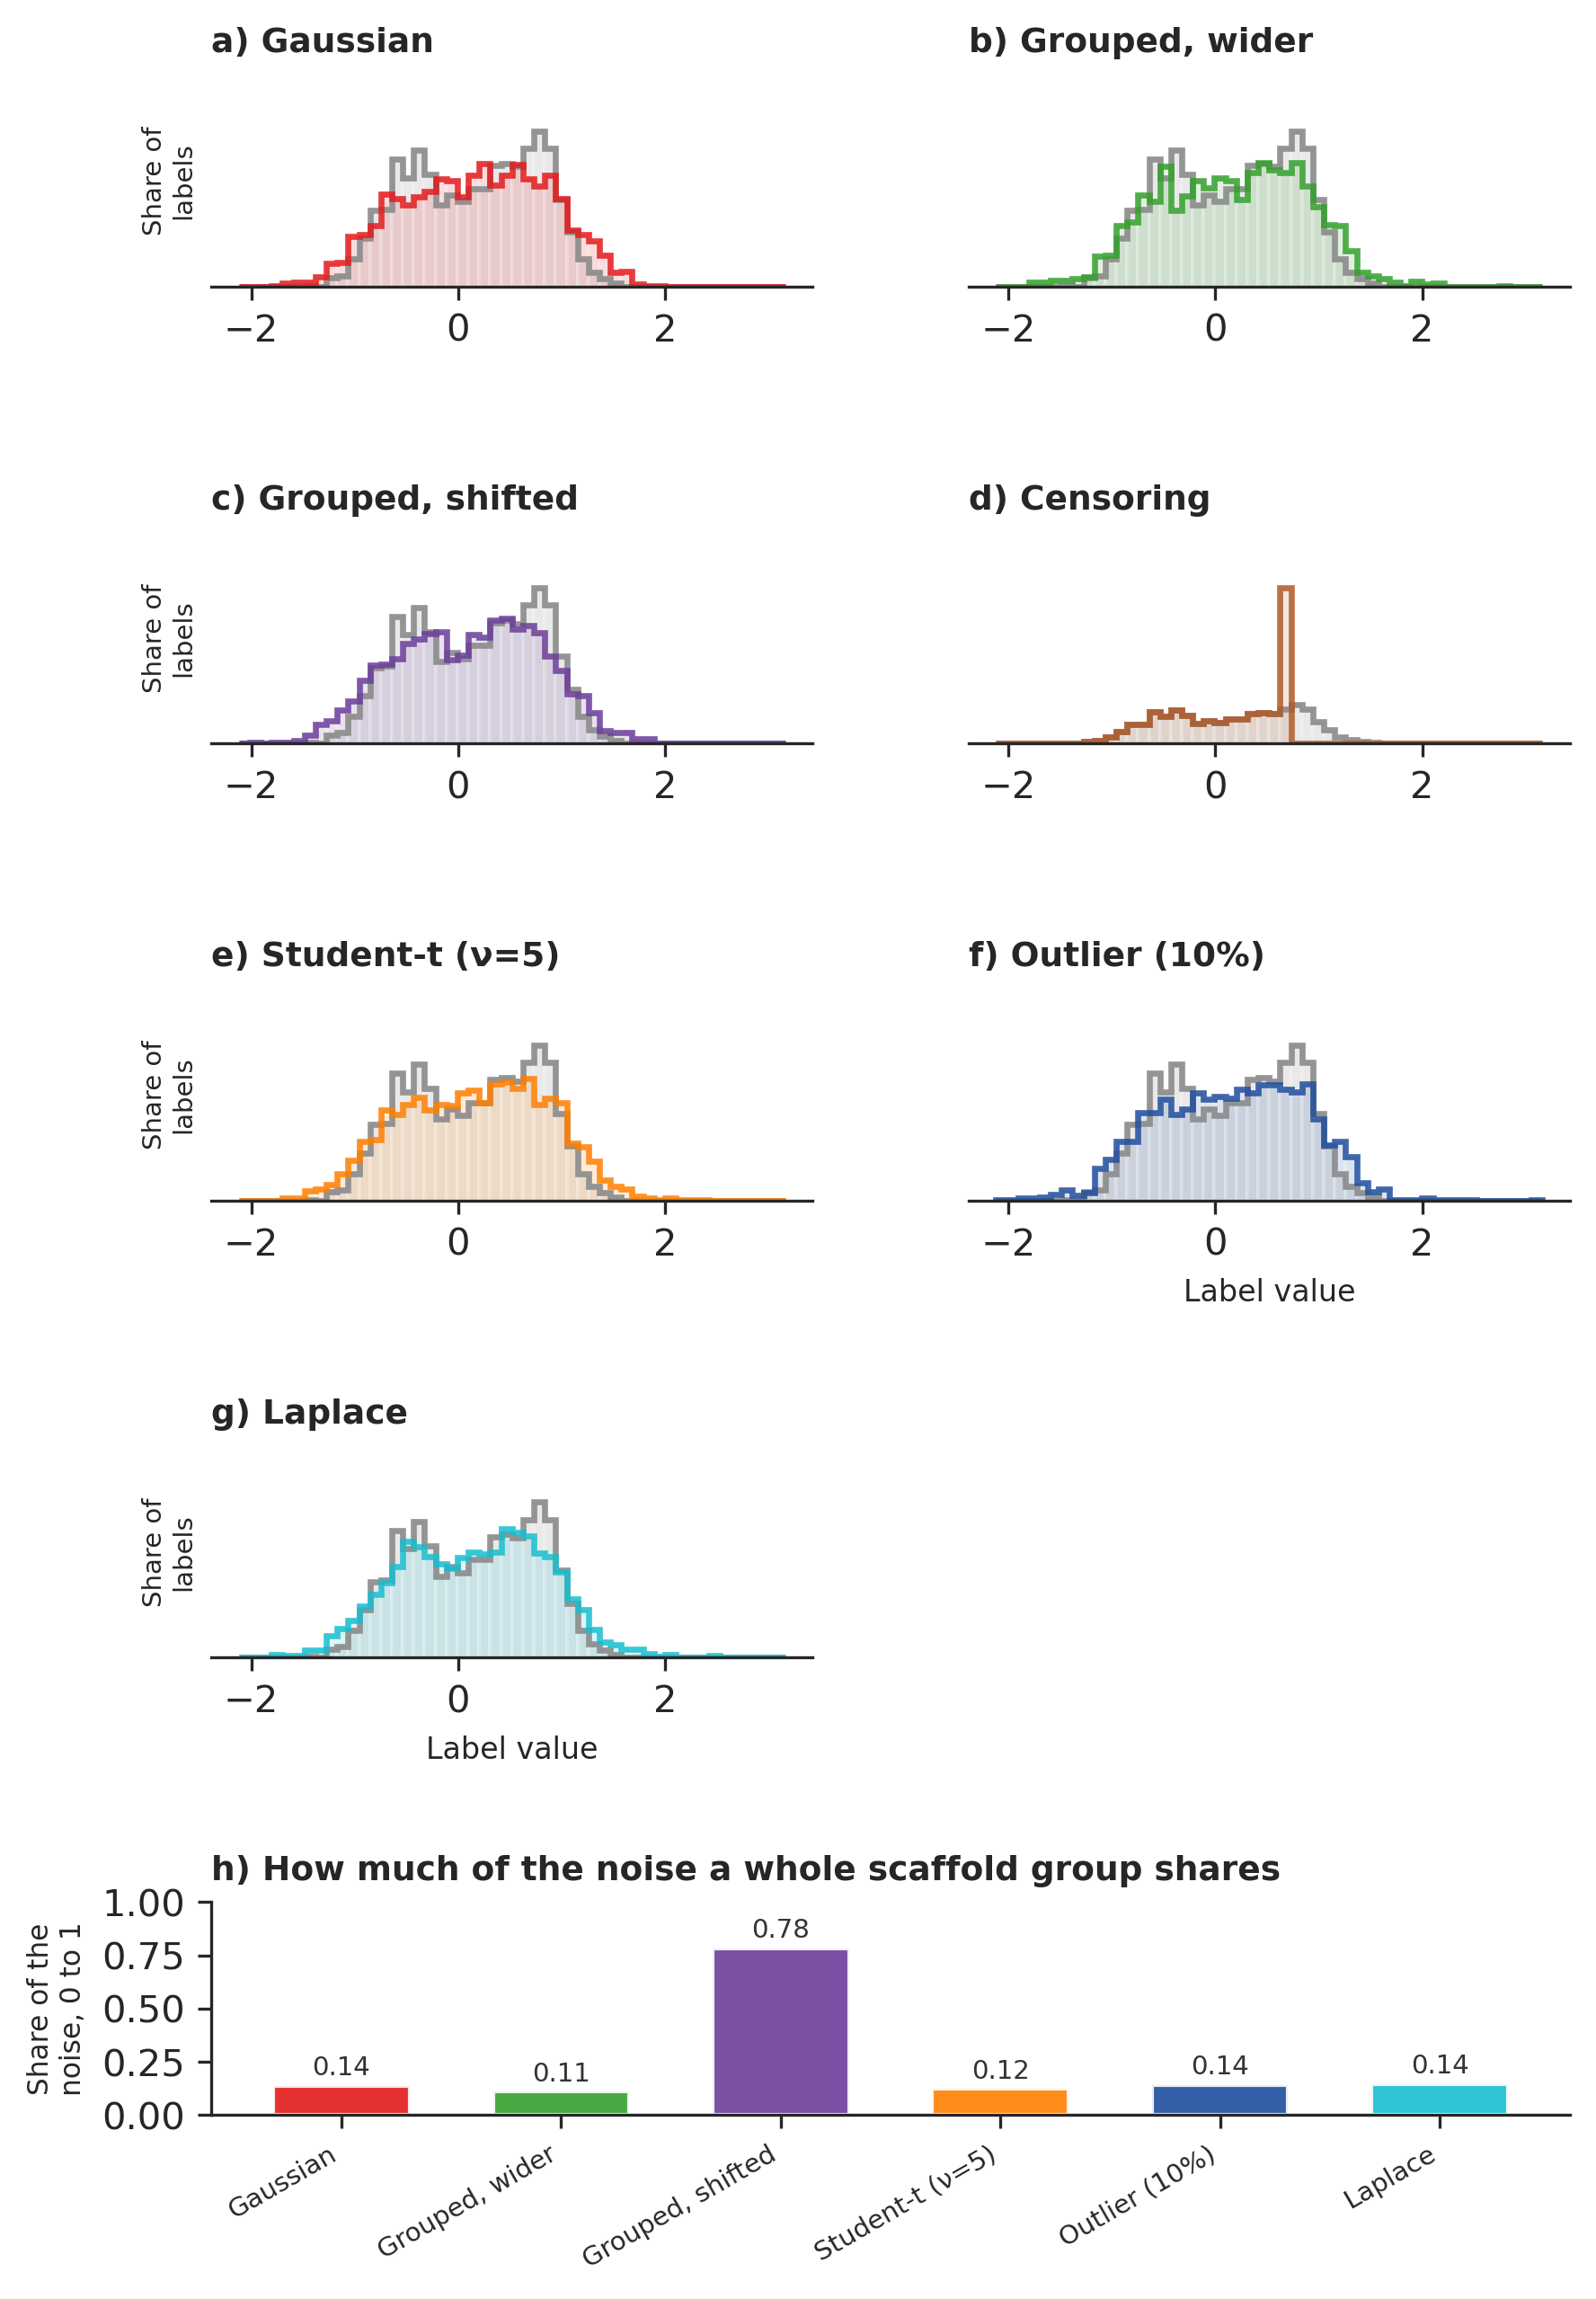
\includegraphics[width=\textwidth,height=0.72\textheight,keepaspectratio]{F1_noise_conditions.png}
\caption[Label distributions under the seven noise conditions.]{Label distributions under the seven noise conditions, for 2,000 synthetic labels in 40 random groups that stand in for scaffold families. a)--g) Clean (gray) and noised (color) labels at a noise level of 0.5 times the standard deviation of the clean labels (25\% of labels clipped under censoring). h) Standard deviation of the mean error within a group divided by that of all errors, for every condition except censoring; a value near 1 means a group's labels move together, and noise that ignores the groups gives about 0.14 with about 50 labels per group.}
\label{fig:noise_conditions}
\end{figure}

For a given label, every condition except censoring delivers the same expected quantity of noise at a set noise level. These levels are defined as a fraction of the standard deviation of clean training labels. The noise added to the label of molecule $i$ is
\begin{equation}
\epsilon_i = \frac{\tau}{G}\,s_i z_i,
\qquad
G = \sqrt{\frac{1}{n}\sum_{j=1}^{n} s_j^{2}}\;\;\sigma_z,
\label{eq:dose_matching}
\end{equation}
Here $\tau$ is the target standard deviation of the noise, in the units of the label, and $z_i$ is
drawn from the condition's distribution at unit scale. The multiplier $s_i$ is $1$ for most
molecules and $\lambda = 3$ for those the condition affects, which are a random 10\% of molecules
under outlier and whole scaffold families covering 20\% of the split under grouped-wider. The
constant $\sigma_z$ is the standard deviation of $z$, equal to $1$ for the Gaussian,
$\sqrt{\nu/(\nu-2)}$ for the Student-$t$ and $\sqrt{2}$ for the Laplace. The factor $G$ divides both
of these out, so that $\epsilon$ has standard deviation $\tau$ in expectation whatever the
distribution and whichever molecules are affected.

Grouped-shifted widens no molecule's error, and instead gives every scaffold family $g$ an offset of
its own,
\begin{equation}
\epsilon_i = \frac{\tau}{G}\left(\sqrt{\rho}\,b_{g(i)} + \sqrt{1-\rho}\,w_i\right),
\label{eq:grouped_shifted}
\end{equation}
with one draw $b$ per family and one draw $w$ per molecule. The two variances sum to $\tau^{2}$, and
the family offset carries a share $\rho$ of that total.

% Original parameter paragraph, now Table tab:noise_conditions:
% We selected parameters from published measurement errors, wherever possible. As inter-laboratory error is estimated to be approximately three times intra-laboratory error, we set $\lambda = 3$ \citep{Avdeef2019}. \citet{Hampel2001} reports that $1-10\%$ of routine scientific data contains gross errors; we selected the upper bound of $10\%$. Laboratory identity accounts for $62\%$ of the variance in Caco-2 across 23 laboratories, prompting us to set $\rho = 0.62$ \citep{Bentz2013}. We took the Student-$t$ and Laplace shapes from the distributions fitted to repeated public bioactivity measurements \citep{Kruger2012}, and contaminated a fraction of the samples with a wider error according to Huber's contamination model \citep{Huber1964}. As we found no published estimate of how large a share of a given dataset inter-laboratory differences affect, we chose to randomly select scaffolds until $20\%$ of the molecules had been covered. 
We selected the parameter values from published measurement errors wherever possible, and Table~\ref{tab:noise_conditions} notes where no published estimate exists.
% TODO: review, needs manual review -- sentence below rephrased from your TODO on the 20%
We found no published estimate of how large a share of a dataset is affected by a difference between laboratories, so under grouped-wider we chose to draw scaffold families until they covered $20\%$ of the training molecules.
\begin{table}[htbp]
\centering
\small
\begin{adjustbox}{max width=\textwidth,max totalheight=0.78\textheight}
\begin{tabular}{@{}P{0.15\linewidth}P{0.30\linewidth}P{0.17\linewidth}P{0.30\linewidth}@{}}
\toprule
\textbf{Condition} & \textbf{What It Changes} & \textbf{Value} & \textbf{Source for the Value} \\
\midrule
Gaussian & Shape: every label's error is Gaussian & -- & The standard assumption in noise-robustness studies \\
% [CLAUDE 2026-10-09] citation fix: Kruger2012 fits no Student-t; nu = 5 has no published source. If nu = 5 was our choice, say so in the text.
Student-$t$ & Shape: heavier tails than Gaussian & $\nu = 5$ & Differences between repeated measurements are non-normal \citep{Kruger2012}; no published estimate of $\nu$ \\
Laplace & Shape: sharper peak and heavier tails than Gaussian & -- & Approximately Laplace for differences in p$K_i$ between related targets, which resemble differences between repeated measurements \citep{Kruger2012} \\
Outlier & Error $\lambda$ times wider on a random share of molecules (Huber's contamination model \citep{Huber1964}) & $10\%$ of molecules; $\lambda = 3$ & $1$--$10\%$ of routine data contain gross errors, upper bound taken \citep{Hampel2001}; inter-laboratory error is about three times intra-laboratory error \citep{Avdeef2019} \\
Grouped-wider & Error $\lambda$ times wider on whole scaffold families & Families covering $20\%$ of the training molecules; $\lambda = 3$ & No published estimate of the share; $\lambda$ as for outlier \citep{Avdeef2019} \\
Grouped-shifted & Every scaffold family gets its own offset; no error is widened & $\rho = 0.62$ & Laboratory identity explains $62\%$ of the variance in log digoxin efflux ratio across the laboratories using cell lines \citep{Bentz2013} \\
Censoring & Labels past a limit are set to the limit; the level is the fraction clipped & Set by the noise level & Censored labels in industrial assays \citep{Svensson2025} \\
\bottomrule
\end{tabular}
\end{adjustbox}
\caption[The seven noise conditions and their parameters.]{The seven noise conditions and their parameter values. $\nu$ is the number of degrees of freedom of the Student-$t$ distribution, $\lambda$ the widening factor (Equation~\ref{eq:dose_matching}) and $\rho$ the share of the noise variance carried by the scaffold-family offset (Equation~\ref{eq:grouped_shifted}). For censoring, the noise level is the fraction of labels clipped.}
\label{tab:noise_conditions}
\end{table}


% CODE INPUT: heading added so the two \ref{sec:lnl_background} in Chapters 4 and 6 resolve. Section level and title need review; no prose written.
\subsection{Learning with noisy labels}\label{sec:lnl_background}
% ---- NOTES: Learning with noisy labels (planned section, no heading yet) ----
% Takeaway: LNL covers every method for training a model when some labels are wrong. Noise mitigation is the subset that changes the labels before training.
% Takeaway: no single method wins, and methods that compare a molecule with its neighbors fail where similarity fails.
% Paragraph 1: what LNL is.
% - Noise mitigation changes, drops or reweights the training labels once, before a model is trained. Any model can then be fitted to the result. Examples: removal, down-weighting, smoothing, relabeling, correction.
% - Noise-robust training leaves the labels and changes how the model trains. Examples: robust losses, noise-modeling layers, regularization, and reweighting inside the training loop (co-teaching, Meta-Weight-Net).
% - A sample-selection step taken out of its training loop and used only to delete molecules before a refit counts as noise mitigation.
% - Noise detection and noise estimation find or size noisy labels. They feed noise mitigation but are not LNL methods themselves.
% - Taxonomy of 62 deep-learning methods in five groups: robust architecture, robust regularization, robust loss function, loss adjustment, sample selection \citep{Song2022}.
% Paragraph 2: why no single method wins.
% - No free lunch: averaged over all problems, no learning algorithm beats another \citep{Wolpert1996, Wolpert1997}.
% - Chemistry analog: twelve algorithms on twelve bioactivity datasets with simulated experimental errors \citep{Cortes2015}.
% - Neighbor-based cleaning goes back to editing a training set by its nearest neighbors \citep{Wilson1972}. It relies on similar molecules having similar labels, which activity cliffs break.
% - QSAR models frequently fail to predict activity cliffs \citep{Dablander2023}.
% - Chapter 6 tests this.
% ---- END NOTES ----

% CODE INPUT
% [CLAUDE 2026-10-09] citation fix: Song2022's categories (iv) loss adjustment and (v) sample selection both act during training; neither is post-processing or pre-training.
LNL covers every method for training a model when some of its labels are wrong, and we divide it into two parts. Noise mitigation changes, drops or reweights the training labels once, before any model is trained, so that any model can then be fitted to the result. Its methods include removal, down-weighting, smoothing, relabeling and correction, and Figure~\ref{fig:data_cleaning} shows how such a method is evaluated. Noise-robust training instead leaves the labels unchanged and alters how the model trains, through robust losses, noise-modeling layers, regularization, or reweighting inside the training loop, as in co-teaching \citep{Han2018} and Meta-Weight-Net \citep{shu2019metaweightnet}. A sample-selection step that is taken out of its training loop and used only to delete molecules before a refit counts as noise mitigation. Noise detection and noise estimation, which find noisy labels or estimate how many there are, feed into noise mitigation but are not LNL methods themselves. \citet{Song2022} provide a comprehensive review of Deep LNL, identifying five main approaches: (i) modifying architectures to better handle noise in training; (ii) employing regularization to reduce overfitting to noise; (iii) adjusting loss functions to be less sensitive to outliers or label flips; (iv) loss adjustment, which corrects, reweights or relabels the loss of each example during training; and (v) sample selection, which identifies examples with correct labels during training, using several networks or several rounds of training.

% CODE INPUT: figure added from ~/Downloads/Data cleaning.png. It shows the example of QM9, a Bayesian model as the
% cleaner and a random forest scored by R^2.
\begin{figure}[!htbp]
    \centering
    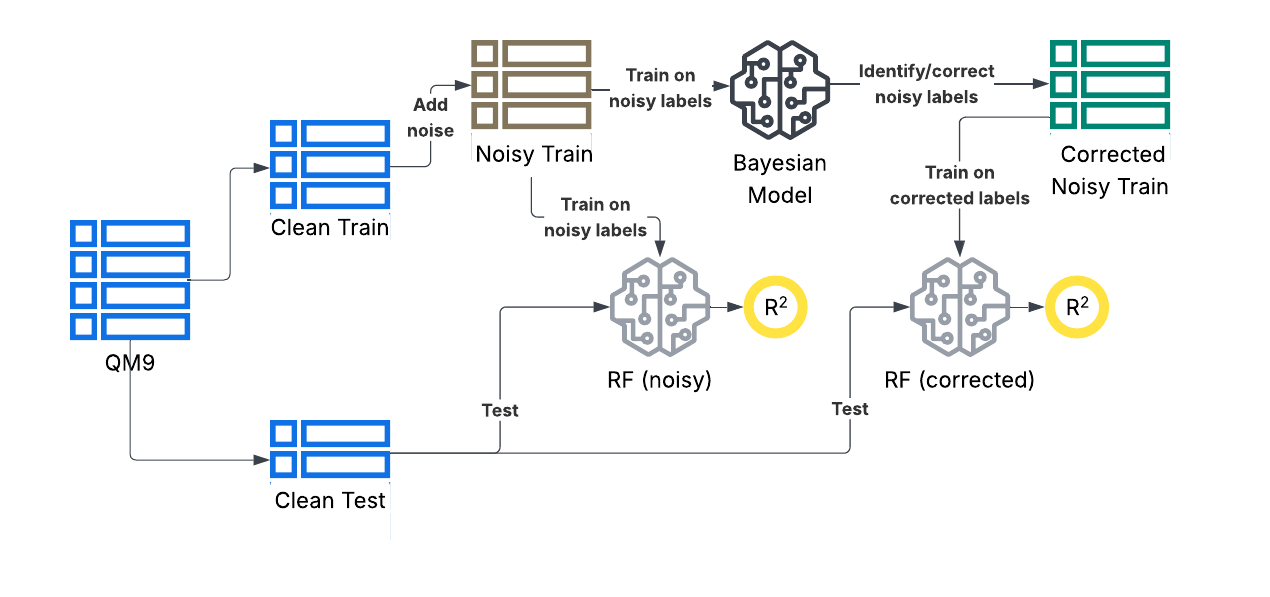
\includegraphics[width=0.95\textwidth,height=0.72\textheight,keepaspectratio]{figures_code_input/data_cleaning.png}
    \caption[Evaluation of a noise mitigation method.]{Evaluation of a noise mitigation method, with QM9 as the example. Noise is added to the training labels only. A random forest trained on the noisy labels is compared with one trained on labels corrected by a Bayesian model, and both are scored by $R^2$ on the clean test set.}
    \label{fig:data_cleaning}
\end{figure}
% CODE INPUT
% TODO: review, needs manual review (Cortes2015 details and the no-universal-solution sentence added from paper.tex)
% [CLAUDE 2026-10-09] citation fix: Wolpert1997 is the no-free-lunch theorem for optimization, not learning.
% [CLAUDE 2026-10-09] citation fix: '10 noise levels' could not be verified (closed access; 15,840 models = 12 x 12 x 110); the abstract reports one clear loser (GBM), not 'no algorithm best'.
No single method is expected to win, since averaged over all problems no learning algorithm outperforms another \citep{Wolpert1996}. \citet{Cortes2015} compared 12 algorithms on 12 bioactivity datasets with increasing Gaussian label noise; gradient boosting was the least tolerant, the other 11 degraded comparably, and two polynomial-kernel models became sensitive only at high noise. This is a recurring theme in LNL research: there is no universal solution to handling noise with experimental endpoints. Neighbor-based cleaning dates back to editing a training set by its nearest neighbors \citep{Wilson1972}, and it relies on similar molecules having similar labels, an assumption that activity cliffs break. QSAR models also frequently fail to predict activity cliffs \citep{Dablander2023}. Chapter~\ref{chap:flaws} tests the assumption that similar molecules have similar labels, and Chapter~\ref{chap:similarity} tests neighbor-based noise mitigation with the hybrid as the feature space.


\section{NoiseInject: a benchmarking framework}
% [notes moved to thesis_notes_moved.md]

% TODO: review, needs manual review
The noise conditions described above are implemented twice. NoiseInject, an open-source Python package, injects the noise on the three assay datasets and computes the robustness and uncertainty metrics, whereas QM9 uses a separate
pipeline, written in Python and Rust, that carries its own Rust implementation of the same conditions.
An automated check compares the two implementations before any experiment is run on the computing cluster. Because the random number generators of Rust and
NumPy produce different streams, the check compares statistics rather
than individual draws. On the same labels, groups and seeds, it compares the delivered noise, the
factor $G$, the median error, the number of badly corrupted labels and the number of molecules
affected.

\subsection{Package description}\label{sec:noiseinject_pkg} % CODE INPUT: label added
% [notes moved to thesis_notes_moved.md]

% TODO: review, needs manual review
NoiseInject (version 1.0.0) evaluates model robustness and uncertainty calibration under artificial
label noise, for both regression and classification. It operates on arrays of labels and on the
predictions of any externally trained model, which makes it model-agnostic, and its core depends only
on NumPy, pandas, SciPy and scikit-learn. Results are returned as \texttt{pandas} data frames with one
row per noise level and one aggregate summary row. The software is available under an MIT license
% [CLAUDE 2026-10-09] citation note: the text says version 1.0.0, but Zenodo's latest NoiseInject release is v0.3.0 (doi 10.5281/zenodo.20532710; all versions 10.5281/zenodo.20531238), titled 'NoiseInject: A Framework for Label Noise Robustness Testing'. Archive 1.0.0, or change the version here and add the DOI to the noiseinject entry.
and archived on Zenodo \citep{noiseinject}.

% TODO: review, needs manual review
\paragraph{Regression noise.} The regression injector specifies a noise shape (Gaussian, Student-$t$ or
Laplace) and a targeting rule (uniform, grouped-wider, grouped-shifted, outlier or censoring)
separately. Each named condition in the package is one combination of the two, together with its
parameters, and this name is recorded with every result. The package defines more settings
than Chapter~\ref{chap:robustness} uses, namely Student-$t$ distributions with $\nu \in \{3, 5, 10\}$ and outlier contamination of $1\%$,
$5\%$ and $10\%$ of molecules. It also defines an outlier variant in which the unselected molecules receive no
noise at all, rather than the base-scale noise of Equation~\ref{eq:dose_matching}.

% TODO: review, needs manual review
The requested noise is the root-mean-square noise $\tau$ in the units of the label, that is, the noise level times the standard deviation of the clean training labels. The
injector computes the per-molecule multipliers $s_i$ and solves for the scale $\tau / G$ in closed
form (Equation~\ref{eq:dose_matching}), so no calibration search is needed. A level of zero returns the
labels exactly unchanged. The affected molecules are selected with a second random number generator,
which is seeded separately from the noise draws and re-seeded on every call. As a result, the affected molecules are
the same at every noise level, including zero, while the noise draws themselves change. Under the
grouped-wider condition, whole scaffold families are added in random order until they cover as close as possible
to $20\%$ of the training molecules, because a fixed fraction of families
gives a very different fraction of molecules when family sizes are uneven.

% TODO: review, needs manual review
The censoring condition is parameterized by the fraction $f$ of labels clipped, and its limit is the $(1-f)$ quantile
of the clean training labels. On the training split, the censored
set is therefore exactly the $k = \mathrm{round}(fn)$ largest labels, whereas on any other split it consists of whichever
molecules lie past the training limit.

% TODO: review, needs manual review
Alongside the noisy labels, each injection returns a record of how they were produced. This record contains the target amount of noise, the factor
$G$, the solved scale, the delivered root-mean-square noise (in label units and as a fraction of the
clean label standard deviation), the mean of $\epsilon$, the fraction of molecules affected, the
number of groups and the largest share held by one group, and the random seeds. The injector also checks the delivered amount of noise.
Because the delivered amount is an estimate from a finite sample, it is compared against a band of three
standard errors,
\begin{equation}
\left|\frac{\hat{\tau}}{\tau} - 1\right| \le \max\!\left(3\sqrt{\frac{\kappa - 1}{4\,n_{\mathrm{eff}}}},\; 0.005\right),
\qquad
n_{\mathrm{eff}} = \frac{\left(\sum_i s_i^2\right)^2}{\sum_i s_i^4},
\label{eq:dose_tolerance}
\end{equation}
where $\hat{\tau}$ is the delivered root-mean-square noise and $\kappa$ is the sample kurtosis of the
unscaled draws $z$, bounded between 3 and 60. The effective count $n_{\mathrm{eff}}$ is the number of
independent contributions over which the delivered amount of noise averages, and it falls below $n$ when the noise is
concentrated on a few molecules. Under the grouped-shifted condition it is
$n_{\mathrm{eff}} = \left(\rho^2/g_{\mathrm{eff}} + (1-\rho)^2/n\right)^{-1}$, with
$g_{\mathrm{eff}} = \left(\sum_g n_g\right)^2 / \sum_g n_g^2$ for family sizes $n_g$. At
$\nu \le 4$ the Student-$t$ distribution has no fourth moment, so the standard error is instead
$1.3\,n_{\mathrm{eff}}^{\,2/\nu - 1}$, with the constant calibrated on the measured spread. A draw
outside the band raises a warning rather than an error. At three standard errors, a correct injector
falls outside the band on about $1\%$ of draws, and the delivered amount is recorded with the result
in either case.

% TODO: review, needs manual review
A second function of the package returns the noise scale that each molecule's region would receive, without drawing any noise.
We use it to score held-out molecules against the pattern of noise to which the training labels were exposed. Under the
uniform and grouped-shifted targeting rules this scale is the same for every molecule, so the package flags the result
as degenerate, because a rank correlation against a constant is undefined and must not be reported as zero.

% TODO: review, needs manual review
A separate injector sizes the noise against a unit supplied by the user rather than against the label standard
deviation. In the experiments implemented in the KIRBy repository, this unit is the standard deviation of a model's out-of-fold residuals on
the clean training labels, so that the noise is sized against the error the model already makes. Its
conditions either add Gaussian noise with variance equal to the level times the square of the unit, or move $2\%$,
$5\%$ or $10\%$ of labels by the level times the unit, with a random sign or always upward. They can also add
Gaussian noise whose standard deviation follows either a per-molecule covariate or a hidden
log-normal draw, and both of these are scaled to the same mean variance as the first condition.

% TODO: review, needs manual review
\paragraph{Classification noise.} The package provides six label-flipping strategies, namely uniform flips,
flip rates set by class frequency, asymmetric flip rates for binary tasks, a random flip rate for each sample,
a separate flip rate for each class, and flips directed by a confusion matrix. Because the realized
flip rate differs from the nominal flip probability under most of these strategies, a binary search
finds the flip probability that produces a target fraction of changed labels.

% TODO: review, needs manual review
\paragraph{Robustness metrics.} For regression, the package computes $R^2$, the root mean squared error (RMSE) and the mean absolute
error at every noise level. For classification, it computes accuracy, together with macro- and weighted-averaged precision, recall and F1
score and a per-class breakdown. Robustness is read from the
retention curve $\mathrm{ret}(x) = m(x)/m(0)$, where $m$ is a bounded metric for which higher values are better
($R^2$ for regression; accuracy, F1, precision or recall for classification) and $x$ is the noise
level. The primary summary is the normalized area under this curve, \aucnorm{} (Equation~\ref{eq:aucnorm} in Chapter~\ref{chap:robustness}),
evaluated by the trapezoid rule. It is the mean fraction of clean performance retained across the
noise levels, lies approximately within $[0, 1]$, and is less directly correlated with clean-label $R^2$ than other robustness metrics we tested. A
secondary summary fits $\mathrm{ret}(x) \approx \exp\!\left(-(x/\tau_W)^{\beta}\right)$ to the curve. The shape parameter
$\beta$ separates curves that hold and then collapse ($\beta > 1$) from curves that fall early and
then plateau ($\beta < 1$), while $\tau_W$ sets the scale of the decay, and the fit requires at least four
noise levels. These two summaries replace the linear slope of performance against noise used in
earlier versions of NoiseInject, which misdescribed a nonlinear curve and was coupled to clean performance. The
package also reports the clean baseline and the retention at the highest noise level. A flag marks any
curve that falls below zero retention, and an optional threshold withholds the curve summaries for
models whose clean baseline is too low for a meaningful degradation.

% TODO: review, needs manual review
\paragraph{Uncertainty metrics.} For a model that returns a predicted standard deviation
$u_i$ for each sample, the package computes several metrics at each noise level. These are the Spearman correlation between $u_i$ and the
absolute error $|y_i - \hat{y}_i|$, the empirical coverage $\frac{1}{n}\sum_i \mathbb{1}\left[|y_i -
\hat{y}_i| \le k u_i\right]$ at $k = 1$ and $k = 2$ against Gaussian targets of $68.3\%$ and
$95.4\%$, the mean interval width $\frac{1}{n}\sum_i 2u_i$, and the expected calibration error (ECE),
\begin{equation}
\mathrm{ECE} = \sum_{b=1}^{10} \frac{|B_b|}{n}\,\left|\bar{u}_b - \overline{|y - \hat{y}|}_b\right|,
\label{eq:ece}
\end{equation}
computed over ten equal-count bins $B_b$ of $u$. All of these metrics are computed on the clean test labels. The Spearman
correlation between $u_i$ and the injected noise $|\epsilon_i|$ can only be computed where the noise
is known, which is on the corrupted molecules, so it requires a separate pair of inputs. It is reported
within each noise level, and a correlation pooled across all levels is returned separately. The pooled value
mostly reflects the fact that uncertainty and noise both rise with the level, so it
does not measure whether a model can identify which molecules are corrupted.

% TODO: review, needs manual review
Three optional wrappers produce $u_i$ from a point predictor. The first applies split-conformal prediction to any
scikit-learn-compatible model, optionally scaled by the label spread of each molecule's nearest
training neighbors. The second fits an exact Gaussian process with a Tanimoto or RBF kernel through \texttt{Gauche}
\citep{gauche}, and the third applies Monte Carlo dropout to any \texttt{PyTorch} network \citep{gal2016}. Example
notebooks and scripts cover regression and classification from start to finish.


\section{Evaluation methodology}
% [notes moved to thesis_notes_moved.md]

% TODO: review, needs manual review
Chapter~\ref{chap:robustness} reports predictive performance as $R^2$ on held-out molecules and robustness as \aucnorm{} (Equation~\ref{eq:aucnorm}). Chapters~\ref{chap:flaws} to~\ref{chap:similarity} state the metric used for each dataset where it is introduced.

\section{Conclusions}

% ---- NOTES: Conclusions ----
% Takeaway: a predictor is a representation paired with a model; Chapter 3 asks which of the two governs how badly a predictor degrades under label noise.
% Paragraph 1: 3-4 sentences.
% - Sentence 1: both halves of a predictor, the representation and the model, have now been introduced.
% - Sentence 2: real assay noise is not independent, identically distributed or symmetric. The artificial noise model has seven conditions. LNL methods have been set out, with noise mitigation as the subset that acts on the labels.
% - No single LNL method wins on every dataset.
% - Sentence 3: NoiseInject injects the conditions and reports robustness and uncertainty metrics. The evaluation section fixes the splits and metrics.
% - Sentence 4: Chapter 3 asks whether the representation or the model architecture governs how badly a predictor degrades under label noise. Point to Chapter 1 for its four questions.
% - Optional: the representations, similarity definitions and noise conditions are reused in Chapters 4 to 6.
% ---- END NOTES ----

% CODE INPUT
% TODO: review, needs manual review -- splits text not yet written; notes in thesis_notes_moved.md
This chapter has introduced both halves of a predictor, namely the representation and the model. Because real assay noise is not independent, identically distributed or symmetric, our artificial noise model comprises seven conditions. We have also set out the methods for LNL, of which noise mitigation is the subset that acts on the labels, and noted that no single method wins on every dataset. NoiseInject injects these noise conditions and reports the robustness and uncertainty metrics, and the section on evaluation methodology fixes the metrics. Chapter~\ref{chap:robustness} asks whether the representation or the model architecture governs how strongly a predictor degrades under label noise, through the four questions set out in Chapter~\ref{chap:intro}. The representations, similarity definitions and noise conditions introduced here are reused in Chapters~\ref{chap:flaws} to~\ref{chap:similarity}.

\chapter{Noise Robustness Across Molecular Representations and Model Architectures}\label{chap:robustness}
% TODO: Chapter 3 update pending. When it lands, search for `TODO: Ch3 update' in Chapters 1, 4 and 7 and re-check each quoted result. Also re-check the Chapter 3 Additional files and the abstract.
% [notes moved to thesis_notes_moved.md]

% TODO: review, needs manual review
% [CODE INPUT: commented out -- the Chapter 3 paper was not submitted, so it is not referenced]
% \textit{Preamble.} The work in this chapter is adapted from Punt, A., Hanser, T., Werner, S., and Morris, G.M., in preparation for the \textit{Journal of Cheminformatics}. Most of the figures, tables, and text in this chapter are therefore either identical or similar to the content of that manuscript. A signed Statement of Authorship for this jointly authored work is included in the front matter.

\section{Introduction}
% [notes moved to thesis_notes_moved.md]

% [CLAUDE 2026-10-09] citation fix: Deng2023's headline is RDKit2D descriptors, not ECFP; \cite as subject changed to \citet.
While there have been many investigations into the effect of noise on molecular property prediction, direction comparisons between how different molecular representations responds to label noise remains limited. The choice of molecular representation certainly affects predictive performance. \citet{Deng2023} evaluated 62,820 models and found that fixed representations, in most datasets RDKit 2D descriptors, outperformed representations learned from SMILES and molecular graphs. Whether these conclusions translate to noise robustness is our question. Between different types of label noise, \citet{Heid2023} found no difference in model performance between error distributions with the same mean and standard deviation. We expand on this by considering alternative patterns of noise, namely noise concentrated in structural groups or on a sparse subset of samples.


This chapter addresses the questions set out in Chapter~\ref{chap:intro}, specifically how the choice of representation and model architecture explain the variance in predictive performance and in noise robustness, what is the impact of the type of label noise, and whether uncertainty estimates track label noise.

\section{Methods}\label{sec:robustness:methods}
% ---- NOTES: Methods ----
% Takeaway: the study crosses four datasets, six representations, 20 model configurations, seven noise conditions and seven noise levels.
% Paragraph 1 (only if the section gets a lead-in paragraph):
% - Four datasets: QM9 (HOMO--LUMO gap) and three assay datasets (logD, Caco-2, hERG K$_i$).
% - Six representations, 20 model configurations, seven noise conditions, seven noise levels.
% - The 20 configurations are thirteen base models and seven variant models. Name both terms here; the Models subsection defines them.
% - The noise conditions are defined in Section~\ref{sec:noise_injection}. Hyperparameters are in Additional file~\ref{app:noise:sec:hyperparameters_default}.
% ---- END NOTES ----

% TODO: remove duplicate -- the second sentence (Gaussian, grouped-wider and grouped-shifted on every pairing, the other four on selected pairings) is now also in Noise Conditions and Levels, from the paper.
We looked at six representations paired with thirteen models, and several variants models, across four prediction tasks. Every pairing was run under Gaussian, grouped-wider and grouped-shifted noise at seven noise levels, and the other four noise conditions (Section~\ref{sec:noise_injection}) were run on selected pairings. The hyperparameters of every model are given in Additional file~\ref{app:noise:sec:hyperparameters_default}.



\subsection{Datasets}

% [CLAUDE 2026-10-09] citation fix: Fediai2023 does not describe what the HOMO-LUMO gap captures; claim and citation removed. Aihara 1999 (J. Phys. Chem. A 103:7487) links a small gap to low kinetic stability, if wanted.
Although we are investigating the effects of label noise stemming from experimental settings, for the purposes of testing we inject controlled amounts of artificial noise into clean labels. Data were extracted from the QM9 molecular property dataset distributed by PyTorch Geometric \citep{Ramakrishnan2014}, which contains 130,831 small organic molecules with pre-computed quantum-mechanical properties obtained from density functional theory (DFT) calculations at the B3LYP/6-31G(2df,p) level of theory. We selected the gap between the highest occupied and the lowest unoccupied molecular orbital (HOMO--LUMO gap) as the prediction target in QM9. We assumed that QM9 labels were free of noise, notwithstanding approximations in the level of theory. Each experiment was replicated 10 times with a distinct random seed and a randomly selected subset of $N = 10{,}000$ molecules, split 80/10/10 into 8,000 training, 1,000 validation and 1,000 test molecules. All models were fitted on those 8,000 training molecules, except the Gaussian processes, which were fitted on a random subset of 5,000 of them; the validation and test molecules were unchanged.

We repeated these experiments on three molecular property datasets with experimentally determined endpoints. From the OpenADMET initiative \citep{openadmet}, we used LogD and Caco-2 efflux permeability, with $N = 5{,}039$ and $N = 2{,}161$ respectively. We also selected hERG $K_i$ data from ChEMBL \citep{Zdrazil2023}, following a protocol inspired by \citet{landrum2024}: filter for binding assays, deduplicate by median pChEMBL value, and remove compounds with an inter-assay standard deviation greater than 1.0 log unit, resulting in $N = 1{,}415$ compounds. Each of the three was partitioned into five folds by grouped $k$-fold cross-validation (CV), and each fold's training block gave up a further grouped fifth as a validation set for early stopping. A model therefore fits between 3,194 and 3,364 of the 5,039 LogD molecules, depending on the fold, so the Gaussian-process subsample never applies to these datasets. Unlike QM9's 10 replicates, which are 10 independent draws from one pool, each assay dataset is a single fixed set in which every molecule is tested exactly once and nothing is redrawn.

All splits and CV folds were grouped by the chirality-blind Bemis--Murcko scaffold, implemented such that each distinct acyclic molecule forms its own group, and groups are filled in random order. Prior to modeling, all molecular structures were sanitized and canonicalized using \texttt{RDKit} to remove invalid valence states and standardize atom and bond typing \citep{rdkit}. Prediction targets were standardized to zero mean and unit variance. Experiments that track uncertainty were run once rather than in replicates.

\subsection{Representations}

% [CLAUDE 2026-10-09] citation fix: kishimoto2023 reports 1,381,747 molecules; 1.34M is from the Hugging Face model card.
In this study, we evaluated six molecular representations: extended-connectivity fingerprints of diameter four (ECFP4), Avalon, Sort \& Slice (SNS), physicochemical descriptors (PDV), ChemBERTa and Molecular Hypergraph Grammar GNNs (MHG-GNNs). The same six were used on QM9 and on the three assay datasets. ECFP4 is a Morgan fingerprint with radius $r = 2$ with $d = 2048$ bits \citep{rogers2010, rdkit}. Sort \& Slice takes the same substructures as ECFP4, but it ranks them by prevalence and selects the top $L$ ($L=1024$) \citep{sns}. We fitted the Sort \& Slice vocabulary on the training molecules alone, refitting it for each QM9 replicate and for each CV fold.  Avalon is a 2,048-bit fingerprint, generated with the Avalon toolkit through RDKit \citep{Gedeck2006, rdkit}. The PDV representation is a vector of 200 physicochemical descriptors computed with RDKit's \texttt{MolecularDescriptorCalculator} \citep{rdkit, Cherkasov2014}; the 200 are listed in Additional file~\ref{app:noise:sec:pdv_descriptors}, and the list is fixed in our code rather than taken from RDKit's default descriptor set, which grows between releases. ChemBERTa embeddings are the mean over the non-padding token embeddings of the \texttt{DeepChem/ChemBERTa-77M-MTR} checkpoint, producing 384 features \citep{Ahmad2022}. MHG-GNNs are a GIN-based autoencoder pre-trained on about 1.38 million PubChem molecules using $\beta$-VAE loss, producing 1024-dimensional embeddings through iterative message passing and found in the published \texttt{mhggnn\_pretrained\_model\_0724\_2023} checkpoint \citep{kishimoto2023}. We z-score normalized PDV, ChemBERTa and MHG-GNN per feature, using the training molecules' mean and standard deviation; ECFP4, Avalon and Sort \& Slice reach the model as built.

\subsection{Models}
% [notes moved to thesis_notes_moved.md]

To understand model behavior in the presence of label noise, we explored a range of model families. We fitted tree ensembles, a support vector machine, Gaussian processes and neural networks. Several are variants of one another, differing in the probabilistic machinery they add, and Additional file~\ref{app:noise:sec:hyperparameters_default} gives every configuration with its settings.

Random Forests (RFs) are one of the most common choices for QSAR modeling thanks to their robustness and interpretability \citep{Svetnik2003}. Quantile Regression Forests (QRFs) hold the distribution of training labels in each leaf and compute quantiles over all trees \citep{Meinshausen2006}. While we used 100 trees for RF, we observed a noisy quantile estimate with 100 trees for QRF, prompting us to use 300 instead. To observe the effect of the quantile mechanism, we then fit a second RF at 300 trees so the two models were identical in all other settings. 

% [CLAUDE 2026-10-09] citation fix: Mustapha2016 and Tian2022 are applications; XGBoost's own paper is Chen2016.
We also used eXtreme Gradient Boosting (XGBoost) \citep{Chen2016}, Light Gradient-Boosting Machine (LightGBM) \citep{ke2017lightgbm}, and Natural Gradient Boosting (NGBoost) \citep{Duan2020}. NGBoost extends deterministic gradient boosting by treating the parameters of a chosen parametric distribution as regression targets and learns them through boosting with a natural gradient update rule \citep{Duan2020}. NGBoost relies on scoring off validation data, which differs by dataset. On QM9 the validation split is already held out of every fit. However, on the three assay datasets the validation set is a scaffold-grouped fifth of the rows NGBoost is handed, which already exclude the validation molecules. 

Support vector machines (SVMs) are a well-established baseline in QSAR modeling \citep{Vapnik1995, Svetnik2003}. We used a radial basis function (RBF) with $C = 1.0$ and $\gamma = \texttt{scale}$ as the kernel, as it accommodates continuous vectors. 

Gaussian processes (GPs) are a non-parametric class of models that use a kernel to produce a Gaussian predictive distribution over every data point \citep{Obrezanova2007, Rasmussen2005}. We fitted three variants of GPs, each with a constant mean and a scaled kernel. The first uses an RBF kernel and runs on all six representations. The second uses the Tanimoto kernel \citep{Ralaivola2005, moss2020} and was run on ECFP4 alone. The third is a heteroscedastic variant in which the RBF process is given a second network that predicts the observation noise of each molecule. One of the major limitations of using GPs in practice is computational scaling; inference has $O(N^3)$ time complexity and $O(N^2)$ memory, where $N$ is the number of training points \citep{Rasmussen2005}. This can be mitigated with sparse GP approximations, but these introduce approximation error and can be more difficult to tune \citep{quinonero2005}. As such, we used a standard GP and only fit on at most $5{,}000$ training molecules, drawn by a seeded sample. Due to the size of the datasets, this cap only affected QM9. We implemented these GP models in \texttt{GPyTorch} \citep{gpytorch}, with the Tanimoto kernel taken from the \texttt{Gauche} framework \citep{gauche}.

We tested two deterministic feed-forward architectures, both fully connected and both implemented in PyTorch \citep{Paszke2019}: (i) NN-$\alpha$ with two hidden layers of sizes 128 and 64, and dropout after each hidden layer and (ii) NN-$\beta$ with two hidden layers, each of size 128, with dropout applied before the output layer. Each model was trained using the Adam optimizer with early stopping on validation loss. We used Bayesian transformations to convert NNs into Bayesian neural networks (BNNs), and implemented them using \texttt{PyTorch} \citep{Paszke2019} with ReLU activations and dropout regularization ($p=0.2$). Additional file~\ref{app:noise:sec:hyperparameters_default} gives their full widths, dropout fractions, learning rates and batch size.

% [CLAUDE 2026-10-09] citation fix: Harrison2024 makes only the last layer Bayesian. It also learns a noise covariance; check the sentence saying VBLL reports only epistemic uncertainty against our implementation.
To get these networks producing uncertainty estimates, we applied four probabilistic transformations to each architecture, producing eight probabilistic networks. The first replaces every linear layer with a Bayesian layer carrying a Gaussian prior $\mathcal{N}(0, 0.1^2)$ on its weights, producing BNN-$\alpha$ and BNN-$\beta$. They are trained on an evidence lower bound whose  Kullback–Leibler (KL) divergence term is divided by the number of training molecules. While this is a straightforward approach, it is computationally expensive. We explored alternative techniques like our second variant, where we add an output head to the standard NN and fit the negative log likelihood of a Gaussian with that variance \citep{kendall2017}. The third, Variational Bayesian Last Layer (VBLL), replaces the output layer with a Bayesian last layer that produces mean-field variational posteriors $q(\mathbf{W}) = \mathcal{N}(\boldsymbol{\mu}_W, \text{diag}(\boldsymbol{\sigma}_W^2))$ over the last-layer weights and trains by maximizing the evidence lower bound. This can be thought of as minimizing the reconstruction loss plus KL divergence $D_{\text{KL}}(q(\mathbf{W}) \| p(\mathbf{W}))$ from a standard normal prior, scaled by $1/N$ \citep{Harrison2024}. Because only its output layer keeps a learned observation-noise parameter, VBLL networks report only epistemic uncertainty. The fourth makes observation noise a function of the input. All eight probabilistic networks estimate their predictive distributions from 100 stochastic forward passes. Each network and its Bayesian counterpart were tuned to the same set of parameters so that NN-$\alpha$ against BNN-$\alpha$ and NN-$\beta$ against BNN-$\beta$ differ by the Bayesian layers alone. 

% TODO: review, needs manual review
The thirteen base models are RF, QRF, XGBoost, LightGBM, NGBoost, SVM, the RBF-kernel GP, and NN, BNN and VBLL in each of the two architectures. The six variant models are the random forest with 300 trees, RF (300 trees); the heteroscedastic GP, GP (het.); the Bayesian networks with a variance head, BNN-$\alpha$ (var.\ head) and BNN-$\beta$ (var.\ head); and the heteroscedastic VBLL networks, VBLL-$\alpha$ (het.) and VBLL-$\beta$ (het.).

\subsection{Noise conditions and levels}
% [notes moved to thesis_notes_moved.md]
% TODO: review, needs manual review
The seven noise conditions used in this chapter are defined in Section~\ref{sec:noise_injection}.

% [CLAUDE 2026-10-09] citation fix: Svensson2025 uses censored labels already in real assays; the clipping protocol and its grid are ours.
We controlled noise quantity using noise levels, representing a fraction of the standard deviation of clean training labels. We ran experiments across seven levels, $0$, $0.2$, $0.3$, $0.5$, $0.75$, $1.0$ and $1.5$. We added the noise to the raw label and standardized the target afterwards, using the clean training mean and spread. To control the quantity of noise for censoring, we recorded every label above the $k$th largest clean training label as that limit and used this level as the fraction clipped, at $0$, $0.1$, $0.2$, $0.25$, $0.3$, $0.4$ and $0.5$. Censoring is common in pharmaceutical assays, where a third or more of labels can be censored \citep{Svensson2025}.

We ran Gaussian, grouped-wider and grouped-shifted noise on every model and representation pairing. The
remaining four conditions ran on selected pairs.

% TODO: model lists in this paragraph are taken from qsar_qm_models/deep_run_pairs.json and censoring_pairs.json (the run configuration), not from the result files; confirm every listed pairing ran.
On QM9, Laplace, Student-$t$ and outlier noise were run on eight models, namely RF, NGBoost, SVM, the GP, GP (het.), BNN-$\alpha$ (var.\ head), VBLL-$\alpha$ (het.) and VBLL-$\beta$ (het.), each on ECFP4, PDV and ChemBERTa. Censoring was run on five pairings, namely RF and GP (het.) on ECFP4, and NGBoost, the GP and BNN-$\alpha$ (var.\ head) on PDV. On the three assay datasets, \aucnorm{} under censoring was computed for the same five pairings, and the uncertainty statistics under censoring for QRF and the other models that give an uncertainty estimate, on ECFP4, PDV and ChemBERTa.
% TODO: in results/decisions_arc_20260916/auc_norm_assay.csv, hERG K_i has four censoring pairings, not five (BNN-alpha (var. head) on PDV is missing), and d7_q4.csv has seven uncertainty models under censoring on the assay datasets; confirm against the final result files.


\subsection{QM9 data pipeline}

QM9 \citep{Ramakrishnan2014}, loaded through PyTorch Geometric, was processed by a separate pipeline where the Python code loads and splits the data, and computes several representations. The data is then passed to the Rust portion of the pipeline which injects the label noise, standardizes the labels, computes the remaining representations, and sends the processed data back to Python which trains and scores the models. 

% TODO: is this not repetitive? Do I not say this elsewhere? 
Each replicate, using its own random seed, randomly selects a subset from QM9, split using scaffold splits. 

. Each of these subsets is split new scaffold split (Datasets subsection), and the same grouping defines the scaffold families targeted by the grouped noise conditions.

% TODO: review, needs manual review
The six representations described above are computed in Python. The run halts if any molecule has an ECFP4 or Avalon fingerprint
that is entirely zero, so that a molecule that failed featurization cannot enter training.

% TODO: review, needs manual review
Traditional approaches load entire datasets into memory from CSV or Parquet files, creating RAM bottlenecks at scale and redundant deserialization overhead across experimental replicates. Our pipeline instead serializes preprocessed data into custom memory-mapped binary files (\texttt{.mmap}) that enable on-demand access with constant low memory footprint regardless of dataset size (Figure~\ref{fig:fig_mmap}). Python writes one file per split, the Rust program reads each file and writes a new one in which the processed labels replace the raw ones, and Python then reads the new files back for training.

% TODO: review, needs manual review
Each memory-mapped file stores a sequence of fixed-format records. A record holds the isomeric and canonical SMILES strings in UTF-8 with a length prefix, the raw target value as a 4-byte float, the requested representations as fixed-width blocks, and the processed target value, which includes the noise and normalization, as a 4-byte float. The blocks occupy 2,048 bytes for Sort \& Slice (1,024 16-bit integers), 800 bytes for PDV (200 32-bit floats), 1,536 bytes for ChemBERTa (384 32-bit floats), 4,096 bytes for MHG-GNN (1,024 32-bit floats), and 256 bytes each for Avalon and ECFP4. Only the requested representations are written, so the byte offset of every field depends on the list of representations. This format permits zero-copy memory mapping, in which Python and Rust access the same disk-backed memory pages without deserialization.

% TODO: review, needs manual review
The Rust program draws the noise for each split separately, following the order in which that
split's records are stored. The noise parameters are set on the training split, since the amount of
noise, the censoring limit and the affected scaffold families are all computed from the clean
training labels. Validation labels receive an independent draw, from a seed derived from the
training seed, with the same amount of noise in label units, the same limit and the same affected
families, and the program verifies that validation received as much noise as training. Test labels
are never corrupted, although every split records the per-molecule noise scale its region would
have received, so that held-out molecules can be scored against the pattern applied in training.

% TODO: review, needs manual review
For every molecule in every split, the Rust program records its canonical SMILES, clean label,
injected noise, noise scale, the noise pattern applied to its region, noisy label and the
standardized value written to file. It also writes a summary of each run that lists the parameters
of the noise condition and the amount of noise delivered. The run halts if the record at any
position holds a different molecule when it is written than when its noise was drawn. A separate
self-test mode applies the same checks on the amount and targeting of noise to a label file,
without running the rest of the pipeline.

% TODO: review, needs manual review
The pipeline then trains the models described in the Models subsection, with the default and tuned hyperparameters given in Additional file~\ref{app:noise:sec:hyperparameters_default}.

\begin{figure}[!htbp]
    \centering
    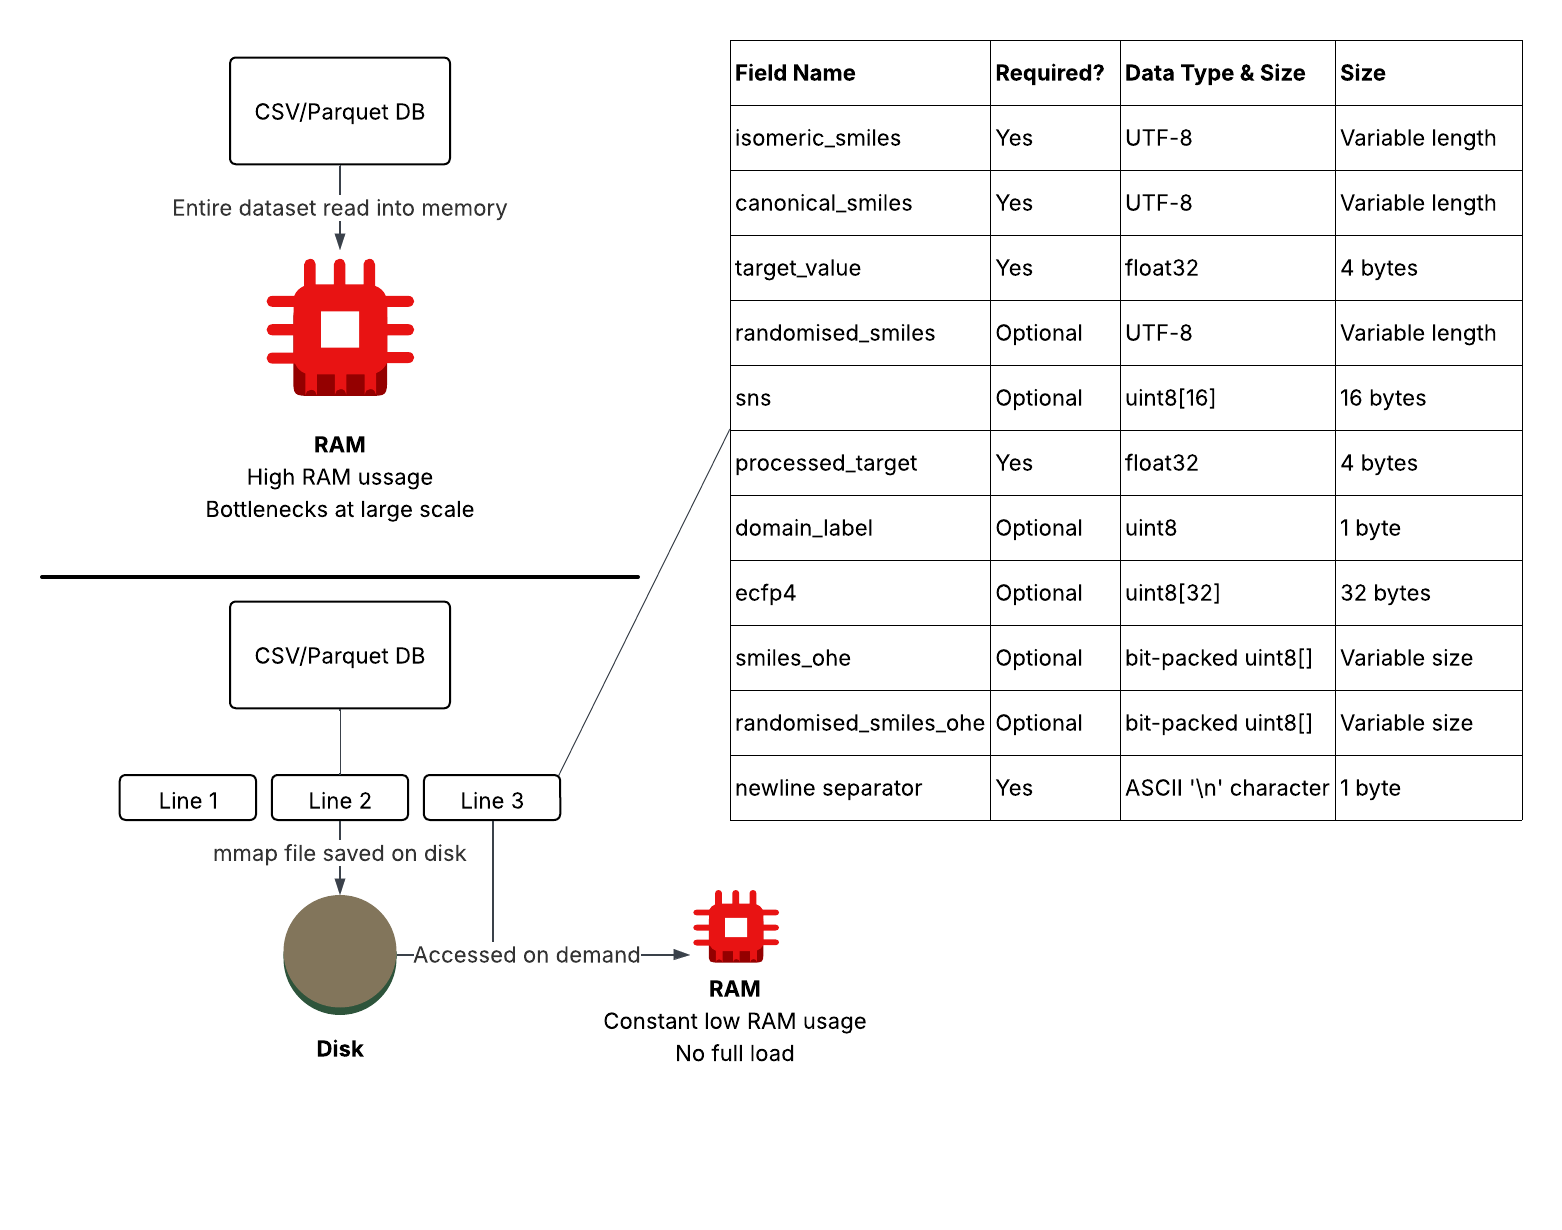
\includegraphics[width=0.95\textwidth,height=0.72\textheight,keepaspectratio]{figure_mmap_structure.png}
    \caption[In-memory and memory-mapped data loading.]{In-memory (top left) and memory-mapped (bottom left) data loading. Memory-mapped loading keeps each molecule as one record of a binary file on disk and reads records into memory on demand. The table on the right lists the fields of one record.}
    \label{fig:fig_mmap}
\end{figure}


\subsection{Uncertainty}
% [notes moved to thesis_notes_moved.md]

Up to this point we have been concerned with how noise affects the predictive performance of QSAR models. However, label noise should also affect the uncertainty these models report. Some models return only a point prediction, while others also return an estimate of uncertainty, either as a predicted distribution or as the spread across an ensemble. Furthermore, some report a single value of uncertainty while others report one that can be decomposed into an aleatoric and an epistemic component \citep{kendall2017}. The aleatoric component describes underlying noise the model associates with the data, while the epistemic component represents the uncertainty within the model's fit. We sought to determine if, as expected, the aleatoric component rises with injected label noise while the epistemic component does not.

For the BNN and VBLL transformations, we took the two components over $T = 100$ stochastic forward
passes \citep{kendall2017}:
\begin{equation}
\hat{u}^2_{\text{ale}}(x) = \frac{1}{T}\sum_{t=1}^{T}\hat{v}_t(x),
\qquad
\hat{u}^2_{\text{epi}}(x) = \frac{1}{T}\sum_{t=1}^{T}\big(\hat{\mu}_t(x) - \bar{\mu}(x)\big)^2 ,
\label{eq:sampling_split}
\end{equation}
where $\hat{\mu}_t(x)$ and $\hat{v}_t(x)$ are the mean and the variance returned for molecule $x$ on
pass $t$, and $\bar{\mu}(x)$ is the mean over passes. Here $\hat{v}_t(x)$ is the predicted observation
noise variance. It varies per molecule in the variance-head and heteroscedastic variants, and is one
number for the whole fit in the VBLL transformation. A full-BNN without a variance head returns no
variance, so its uncertainty is epistemic alone.

The other models follow the same split. For GPs, the epistemic component is the posterior variance of the latent function and the aleatoric component is the learned observation noise \citep{Rasmussen2005}. All variants of the GP produce one number for the whole fit except heteroscedastic. For QRF models, each tree holds multiple training molecules. So for a given molecule, the aleatoric component is the variance the labels the molecule's given leaf. The total aleatoric uncertainty are those variances averaged over the trees. The epistemic component is the variance of the leaf means across the trees. NGBoost predicts one variance for each molecule from a single fit, which is aleatoric alone \citep{Duan2020}. In every model, the total uncertainty is the sum of the aleatoric and epistemic components.

No held-out label carries injected noise, so every comparison against the injected noise was made on
training molecules. Each training set was divided into five folds grouped on Murcko scaffolds, and each
molecule was scored by a refit that excluded its own fold. For NGBoost on QM9, three of the five folds
were scored to limit its cost. No uncertainty was calibrated after fitting.


\subsection{Evaluation}
% [notes moved to thesis_notes_moved.md]
We compute statistics on the held-out molecules, for QM9 the test split and for three assay datasets the held-out fold of the scaffold CV. Different combinations of dataset, model, representation, noise condition, and noise level are examined in each scenario. We used the coefficient of determination ($R^2$) throughout. For molecule $i$, let $y_i$ be the clean label, $\hat{y}_i$ the prediction, $\epsilon_i$ the noise injected into its label and $u_i$ the predicted uncertainty.

To evaluate the effect of label noise, we tracked predictive performance retention under increasing artificial noise. For each QSAR pairing we recorded $R^2(\tau)$ at each noise level $\tau$, and normalized it to obtain the retention ratio $R^2(\tau)/R^2(0)$. To quantify robustness, we used the normalized area under this retention curve,
\begin{equation}
\aucnorm = \frac{1}{\tau_{\max}} \int_0^{\tau_{\max}} \frac{R^2(\tau)}{R^2(0)}\, d\tau,
\label{eq:aucnorm}
\end{equation}
evaluated using the trapezoidal rule over the seven noise levels, $\tau \in \{0,\allowbreak 0.2,\allowbreak 0.3,\allowbreak 0.5,\allowbreak 0.75,\allowbreak 1.0,\allowbreak 1.5\}$, in the units of Equation~\ref{eq:dose_matching}. While we tested other metrics of robustness, we found \aucnorm{} to be less directly correlated to clean-label $R^2$ predictions. For censoring, we sweep over a set of fractions to clip the labels prior to normalization. 

An \aucnorm{} value near 1 indicates that the QSAR model in question has retained predictive performance with artificial noise, meaning it is more robust to noise. Since we normalize the curve by its own clean-label predictive performance, a model with a low clean $R^2$ has less to lose, so \aucnorm{} is reported beside clean $R^2$. We excluded replicates with a clean $R^2 < 0.3$ from the robustness analysis (Additional file~\ref{app:noise:sec:excluded_configurations}), as performance retention ratios become unstable when the clean-label denominator approaches zero. On QM9 one \aucnorm{} is computed per replicate, and we report the median over the 10 replicates. On the three assay datasets one value is computed per scaffold fold, and the median over the five folds is reported. 

To compare the relative effect of the 13 base models across datasets and noise conditions, we compared their rankings using Spearman's rank correlation coefficient ($\rho$) between clean $R^2$ and \aucnorm. We compared probabilistic models  with its deterministic counterpart using a two-sided Wilcoxon signed-rank test paired on the replicate, at $\alpha = 0.05$, separately for each representation and noise condition. This test was run only on QM9, as with five scaffold folds the
smallest attainable $p$ is 0.0625.

We conducted a separate analysis of variance (ANOVA) for each noise condition to identify the
relative contributions of molecular representation and model architecture to both predictive
performance and noise robustness. For a given metric $y$, either $R^2$ at a noise level of 1.0 or
\aucnorm:
\begin{equation}
y_{fmjr} = \mu + s_r + \alpha_f + \gamma_{m(f)} + \beta_j + (\alpha\beta)_{fj} + (\gamma\beta)_{m(f)j} + e_{fmjr},
\end{equation}
where $s_r$ represents the effect of replicate $r$, $\alpha_f$ represents the effect of model family $f$, $\gamma_{m(f)}$ represents the effect of model architecture $m$ within its family, $\beta_j$ represents the effect of
molecular representation $j$, $(\alpha\beta)_{fj}$ and $(\gamma\beta)_{m(f)j}$ are the interaction terms, and $e_{fmjr}$ is the
residual. The proportion of variance explained by each term was calculated as the
effect size
\begin{equation}
\eta^2_{\text{term}} = \frac{SS_{\text{term}}}{SS_{\text{total}}},
\end{equation}
using Type I (sequential) sums of squares, entered in the order replicate, model family, model architecture within family, molecular
representation, interaction. The 10 QM9 replicates provide the residual. The uncertainty on each share is the 95\% interval of $\eta^2$ over 1,000 bootstrap resamples of whole replicates. These shares describe the models and representations tested here, not the choice of model or representation in general. 

ANOVA relies on the assumption that observations both within and across groups are independent. Two features of this study break that assumption. First, each QM9 replicate uses the same data split and the same noise draw for every model and representation, so observations from one replicate are not independent of each other; we therefore entered the replicate as a block. Second, across the whole set of models in this study, some pairs produced similar predictions that are not independent, so a method present in several near-identical versions would count several times towards the share of model architecture. To handle this issue, we grouped the models into families. We considered grouping pairs of models that share a method or an architecture, and compared each pair on clean $R^2$ and on \aucnorm{} under the three noise conditions run on every representation, separately on each of the six representations, which gives 24 comparisons per pair. A pair was grouped when the mean difference between the two models was smaller than their standard deviation across replicates in at least two thirds of these comparisons (Additional file~\ref{app:noise:sec:model_redundancy}). Five families met this criterion: RF with quantile regression forests (QRF; 16 of 24), XGBoost with LightGBM (23 of 24), NN-$\alpha$ with BNN-$\alpha$ (20 of 24), NN-$\beta$ with BNN-$\beta$ (18 of 24), and VBLL-$\alpha$ with VBLL-$\beta$ (20 of 24). VBLL did not group with the plain or Bayesian network of its own architecture (4 to 10 of 24), as its clean $R^2$ was lower by 0.02 to 0.09, and NGBoost did not group with XGBoost or LightGBM (2 and 3 of 24). The two architectures of the plain networks, and of the Bayesian networks, also met the criterion (18 and 17 of 24); we grouped by architecture instead, which the evidence supports equally well. The 13 base models therefore form eight families. Within these families, the differences between models accounted for at most 1.0\% of the variance in any outcome and noise condition on QM9, and up to 15.1\% of predictive performance on clean labels on the three assay datasets. We also ran Tukey's honestly significant difference test between the members of each family, separately for each representation (Additional file~\ref{app:noise:sec:tukey_within_families}). With 10 replicates it detects differences smaller than the variation between replicates, so we report it beside the size of each difference rather than use it to form the families.

Across representations, we considered grouping SNS with the ECFP4 fingerprint, as both encode overlapping circular substructure information. The two differed by more than their variation across replicates on clean $R^2$ for every model (0 of 13), so all six representations were kept as separate levels (Additional file~\ref{app:noise:sec:representation_redundancy}).

To assess the interaction between uncertainty estimation and label noise, we posed three questions. First, whether uncertainty rise with label noise, as measured by the mean $u_i$ over held-out molecules at the highest noise level
divided by its value with no added noise, in each replicate or fold. The second pertains to models who report separate aleatoric and epistemic components. We divided the increase of mean epistemic uncertainty between the highest level of noise and clean labels by the mean of the aleatoric component to determine how each responds to label noise. A ratio near 0 means the added noise was attributed to the labels while a ratio of 1 or above means the epistemic component grew as much or more. We also compared the mean aleatoric component with the standard deviation of the injected noise. The third question we had was whether per-sample uncertainty values track injected label noise, as measured by the Spearman correlation between $u_i$ and $|\epsilon_i|$ over out-of-fold training molecules, per fold and per noise level. We also report the Spearman correlation between $u_i$ and the absolute error of the prediction. Finally, we asked whether dividing a molecule's out-of-fold absolute error by $u_i$ ranks the corrupted labels better than the error alone, and report the difference between the two Spearman correlations with $|\epsilon_i|$.


\section{Variance decomposition}

Considering the two main components of a QSAR model, the molecular representation and the model architecture, we sought to understand how each contributes to both predictive performance and noise robustness. ANOVA decomposition divides the variance between model family, model architecture within its family, molecular representation, the pairing of the two, the replicate, and a residual. We ran this decomposition for Gaussian noise, the standard model, as well as methods whose injected noise is related to the feature space, grouped-wider and grouped-shifted (Figure~\ref{fig:variance}, Table~\ref{tab:variance}). For predictive performance measured in $R^2$ at a noise level of 1.0, model family and molecular representation account for comparable shares of the variance, 26.6\% and 29.0\% under Gaussian noise. However, for noise robustness, quantified by the normalized area under the R$^2$ retention curve (\aucnorm; higher values indicate greater robustness), model family accounts for 47.2\% of the variance while molecular representation for 8.1\%. This pattern is observed across noise conditions and makes sense, as label noise does not impact the features. The interaction between model and molecular representation explains 19.9\% of the variance in \aucnorm, more than twice the 8.1\% explained by representation alone, meaning  representation acts on noise robustness mainly through the model it is paired with. As such, we primarily compare representations within each model.

\begin{figure}[!htbp]
\centering
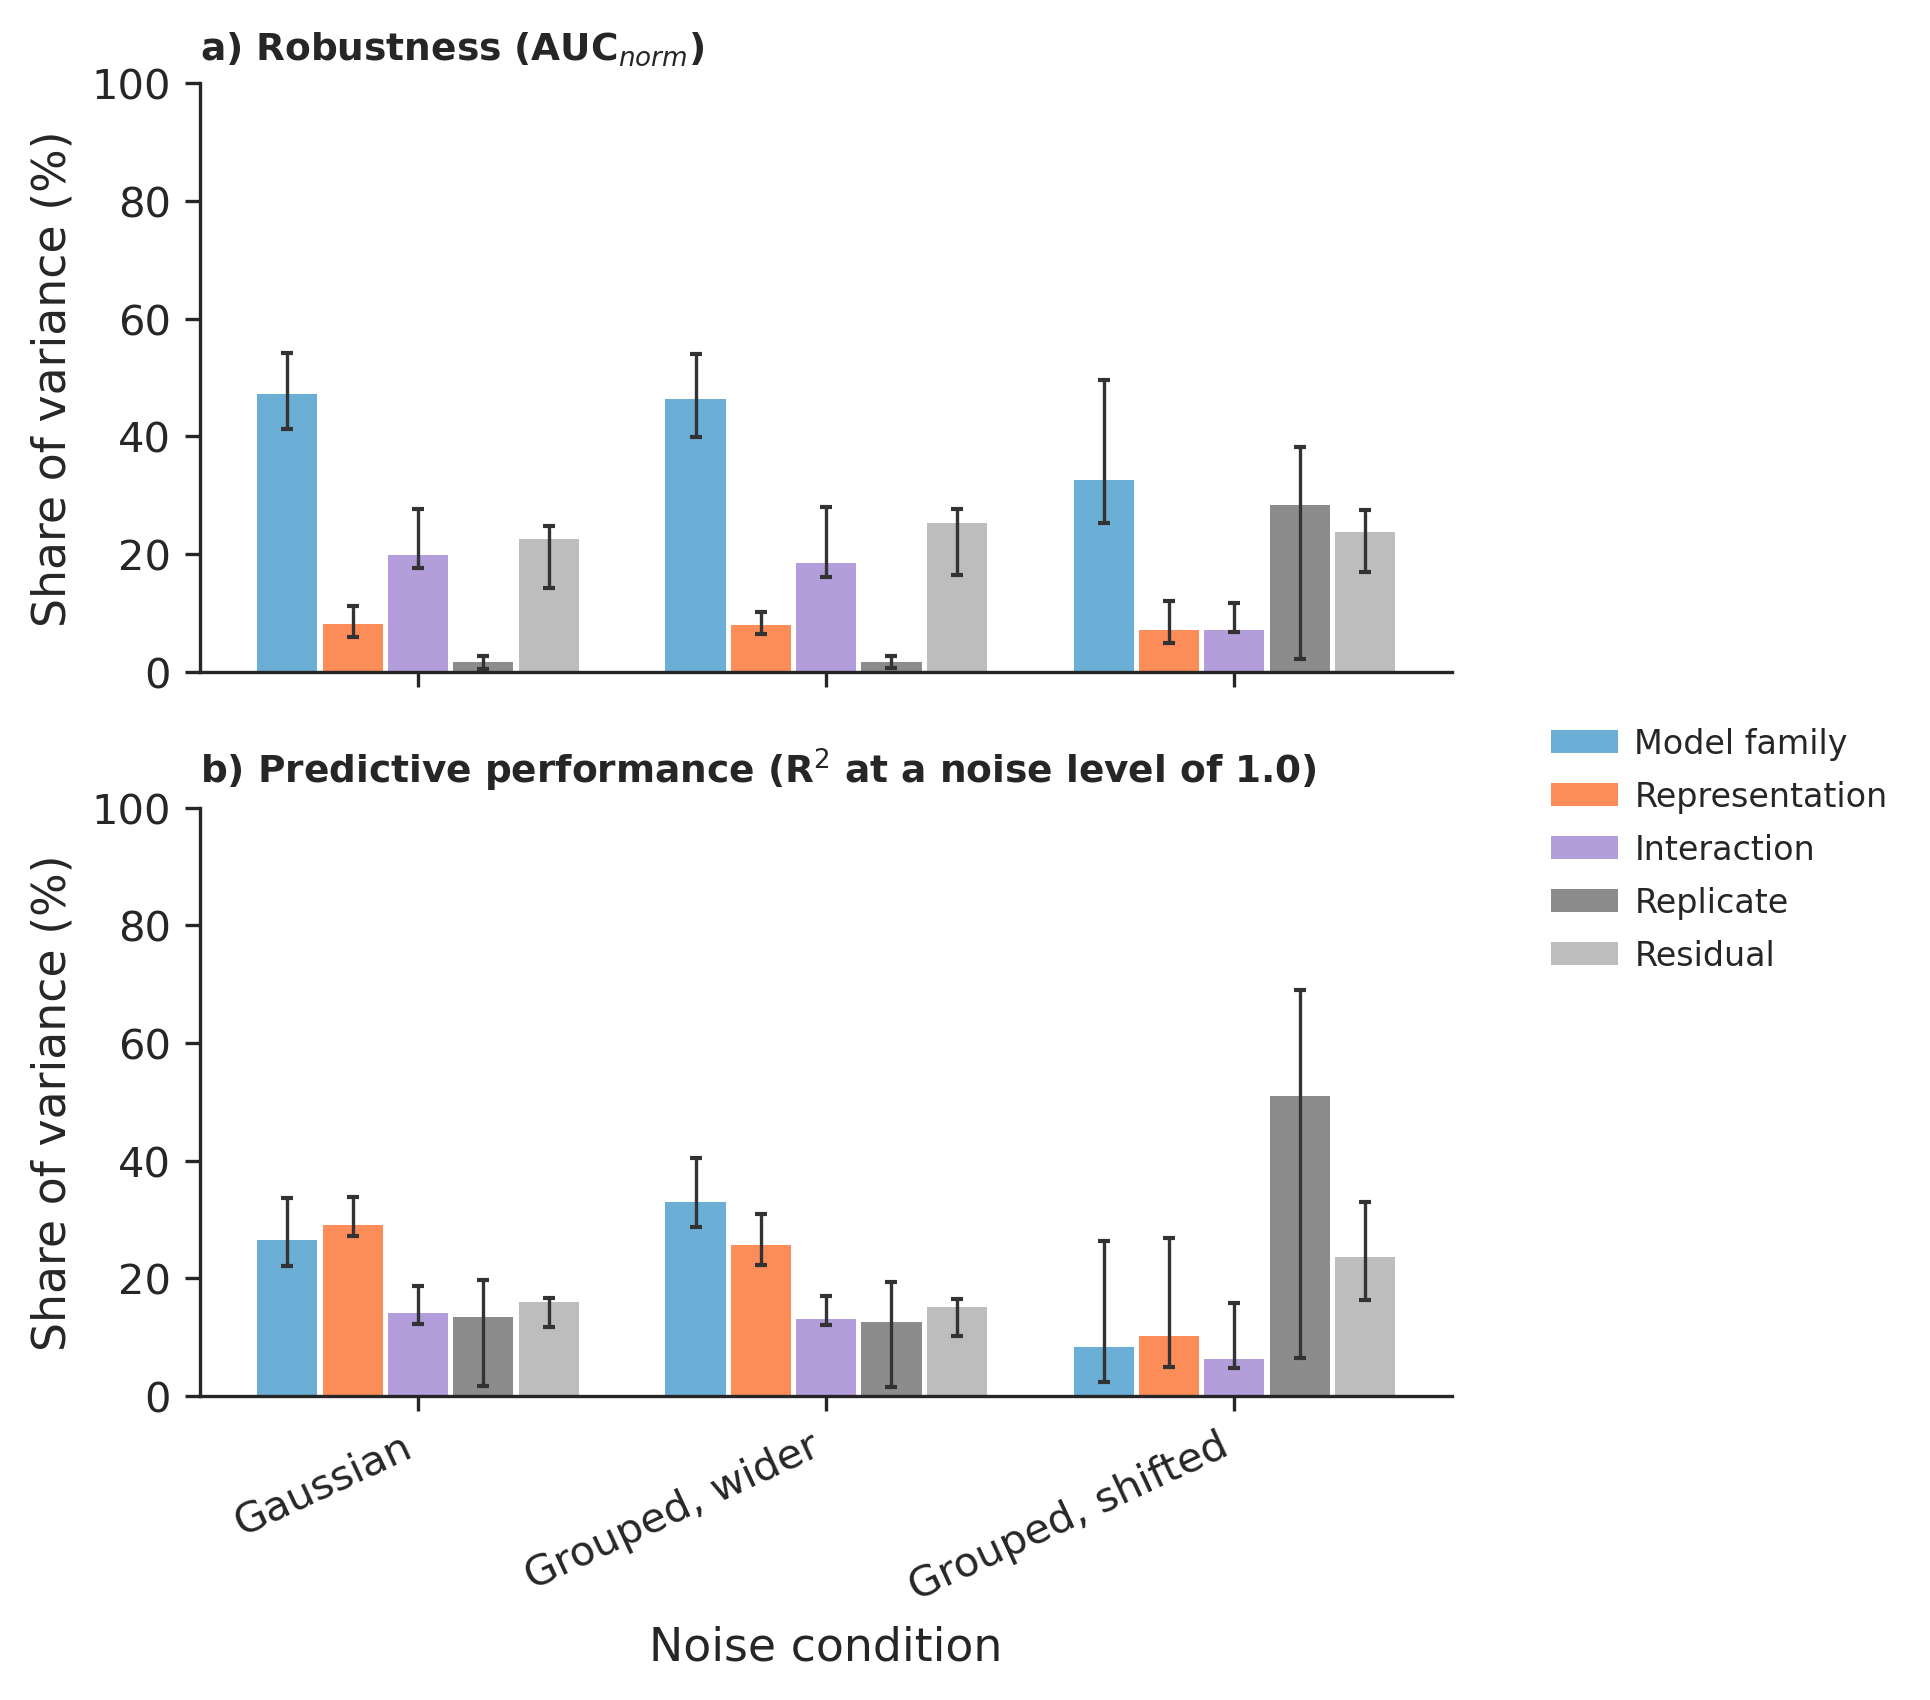
\includegraphics[width=\textwidth,height=0.72\textheight,keepaspectratio]{F2_variance_decomposition.png}
\caption[Variance decomposition of robustness and predictive performance on QM9.]{Share of the variance explained by each term, on the QM9 HOMO--LUMO gap: a) robustness (\aucnorm);
b) predictive performance ($R^2$ at a noise level of 1.0). Whiskers are 95\% bootstrap intervals over replicates. Model within family, at most 1.0\% in every decomposition on QM9, is not drawn.}
\label{fig:variance}
\end{figure}

We compare the variance decomposition on both clean and noisy labels (Figure~\ref{fig:three_outcomes}a). For predictive performance, the artificial label noises lowers the impact of the choice of model family, while the replicate and residual take more. This means that the variance is left more up to chance and to the underlying variation within the data itself with label noise, which is the expected behavior. Robustness divides the variance a bit differently. Representation explains 8.1\% of the variance in \aucnorm, against 31.1\% of clean $R^2$, while model family rises to 47.2\%. The replicate nearly disappears from \aucnorm, likely because each replicate's curve is divided by that replicate's own clean $R^2$, so a difficult split lowers both and cancels out.

We include two terms which stem from the data rather than the model, the residual and replicate terms. The replicate measures how much of the variance can be attributed to the train and test split, which in this case is a scaffold split. On QM9 we replicated each experiment 10 times with different random draws of $N=10{,}000$, each time giving a new scaffold split. On the assay datasets, a replicate refers to one of the five scaffold CV folds. A large replicate term in ANOVA indicates that the folds differ from one another. The residual is variance that no other term accounts for.

\begin{figure}[!htbp]
\centering
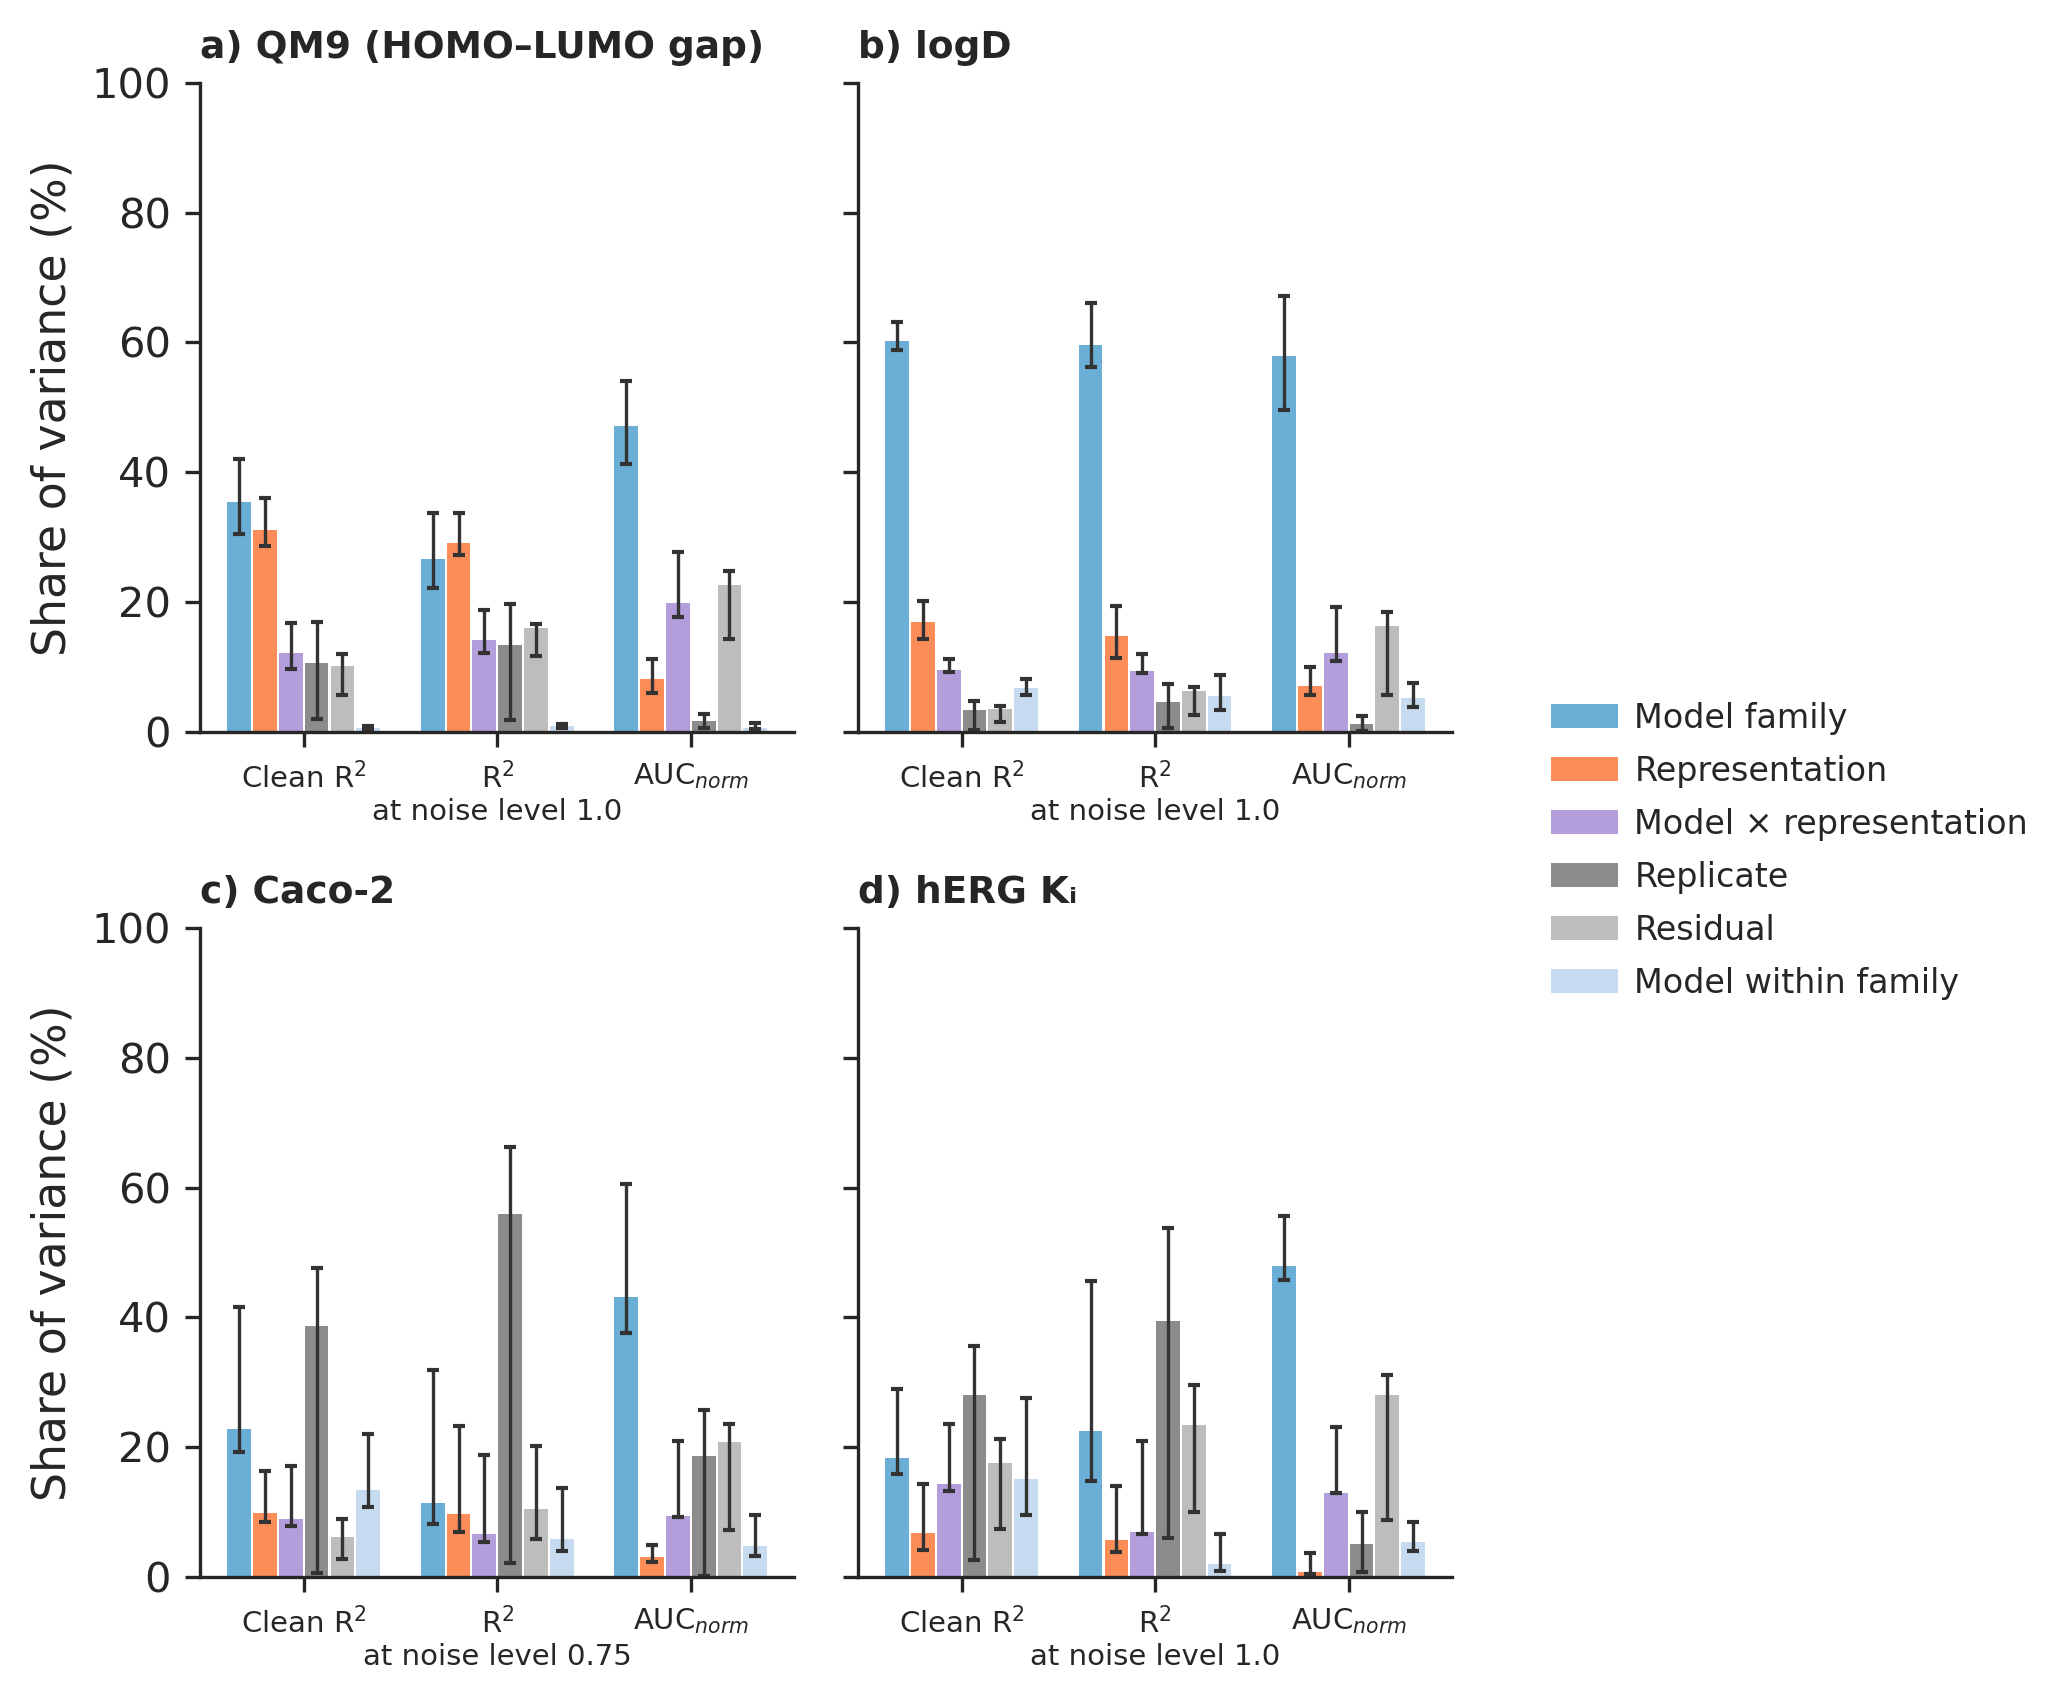
\includegraphics[width=\textwidth,height=0.72\textheight,keepaspectratio]{F2d_three_outcomes_every_dataset.png}
\caption[Variance shares of clean performance, noisy performance and robustness on all four datasets.]{Share of the variance explained by each term on a) the QM9 HOMO--LUMO gap, b) logD, c) Caco-2 and d) hERG $K_i$, for clean $R^2$, and for $R^2$ at a noise level of 1.0 (0.75 on Caco-2) and \aucnorm{} under Gaussian noise. Whiskers are 95\% intervals from 1,000 bootstrap resamples of replicates: 10 on QM9 and five scaffold folds on each assay dataset. The values and their intervals are in Additional file~\ref{app:noise:sec:variance_intervals}.}
\label{fig:three_outcomes}
\end{figure}

While we observe similar patterns between noise conditions, the predictive performance of grouped-shifted noise in particular varies significantly between replicates, resulting in a larger share for the replicate. We find that 28.4\% of the variance in \aucnorm{} and 51.0\% of the variance in $R^2$ are due to the replicate, with model family falling to 32.7\% and 8.4\%. This indicates that the offset applied to each scaffold may account for more of the variance in both R$^2$ and \aucnorm.

\begin{table}[!htbp]
\centering
\small
\setlength{\tabcolsep}{3pt}
\begin{adjustbox}{max width=\textwidth,max totalheight=0.78\textheight}
\begin{tabular}{lcccccc}
\toprule
Condition & Outcome & Replicate & \begin{tabular}[b]{@{}c@{}}Model\\family\end{tabular} & Representation & Interaction & Residual \\
\midrule
None & Clean R$^2$ & 10.6 & 35.4 & 31.1 & 12.1 & 10.2 \\
Gaussian & \aucnorm{} & 1.7 & 47.2 & 8.1 & 19.9 & 22.6 \\
Grouped, shifted & \aucnorm{} & 28.4 & 32.7 & 7.0 & 7.2 & 23.7 \\
Grouped, wider & \aucnorm{} & 1.7 & 46.3 & 7.9 & 18.5 & 25.3 \\
Gaussian & R$^2$ at level 1.0 & 13.4 & 26.6 & 29.0 & 14.2 & 16.0 \\
Grouped, shifted & R$^2$ at level 1.0 & 51.0 & 8.4 & 10.3 & 6.2 & 23.7 \\
Grouped, wider & R$^2$ at level 1.0 & 12.7 & 33.0 & 25.7 & 13.1 & 15.1 \\
\bottomrule
\end{tabular}
\end{adjustbox}
\caption[Variance decomposition by noise condition on QM9.]{Share of the variance (\%) explained by each term on the QM9 HOMO--LUMO gap, for 13 base models and six
representations over 10 replicates. Model within family, at most 1.0\% in every row, is left out, so a row does not sum to 100\%. Intervals are in Additional file~\ref{app:noise:sec:variance_intervals}.}
\label{tab:variance}
\end{table}

\section{Predictive performance and noise robustness}

The variance decomposition tells us what aspect of QSAR modeling affects predictive performance and robustness, however it does not tell us about the characteristics of individual models. All model's performance degrades as the labels get increasingly corrupted with noise (Figure~\ref{fig:curves}). The loss remains small until the artificial noise reaches about half the spread of the clean training labels, and then it begins to drop. The rate it drops and the quantity of noise retained is not necessarily correlated to the model's predictive performance on clean labels. Across the 13 base models under Gaussian noise at ECFP4, clean $R^2$ and \aucnorm{} rank in opposite directions at a Spearman correlation of $-0.10$ ($p = 0.73$) (Figure~\ref{fig:decoupling}). If anything, the lower a model's predictive performance on clean labels, the less it has to lose as the labels get noisier.

The link between predictive performance and noise robustness can be examined by model family (Figure~\ref{fig:decoupling}). The forests, boosted trees, SVM, and GP all retain relatively high predictive performance on clean labels while maintaining relatively strong robustness to noise. The plain NNs and BNNs are among the highest in predictive performance on clean labels, and are the four least robust. The two variational networks sit between these groups, with lower predictive performance on clean labels and middling noise robustness. Standard feed-forward networks can make strong predictions under clean labels, however they are not a safe bet under noisy ones.

NGBoost is a standout case in the sense it is highly dependent on its paired molecular representation. Under Gaussian noise it has the highest \aucnorm{} on every one of the six representations, yet also the lowest in predictive performance on four of the six representations. It is one of the worst performing models with respect to $R^2$ on clean data. Its high robustness is partially due to the fact that when you start with a low predictive performance, you don't have as much to lose. However, it maintains shallow robustness curves across representations. On ECFP4 NGBoost's predictive performance ranks lowest up to a noise level of 0.75 and stays in the lower half at every noise level. However, on PDV it starts second lowest and ends highest, surpassing the other models between noise levels 1.0 and 1.5. So when paired with the right features, NGBoost has the potential to make better predictions under higher quantities of label noise. On group-shifted noise, RF has higher \aucnorm{} values than NGBoost on ECFP4, Avalon and ChemBERTa. Even then, NGBoost reports the highest noise robustness for PDV, MHG-GNN and Sort \& Slice. While NGBoost performs well under higher label noise, LightGBM performs well under smaller quantities of noise. Its performance drops sharply after noise level 1.0.

As we've seen, the choice of representation can have an impact on noise robustness, but that impact is determined by model family, represented by the interaction term between model and representation in Figure~\ref{fig:grid}. Some models are more impacted by representation than others, though. In general, networks span a wider range of \aucnorm{} across the six representations than any of the other models. Between ECFP4 and PDV under Gaussian noise, the four plain and Bayesian networks differ by between 0.037 and 0.065 of \aucnorm, while no tree or kernel model shifts by more than 0.011. VBLLs are an exception, as no two variational networks differ by more than 0.019.

\begin{figure}[!htbp]
\centering
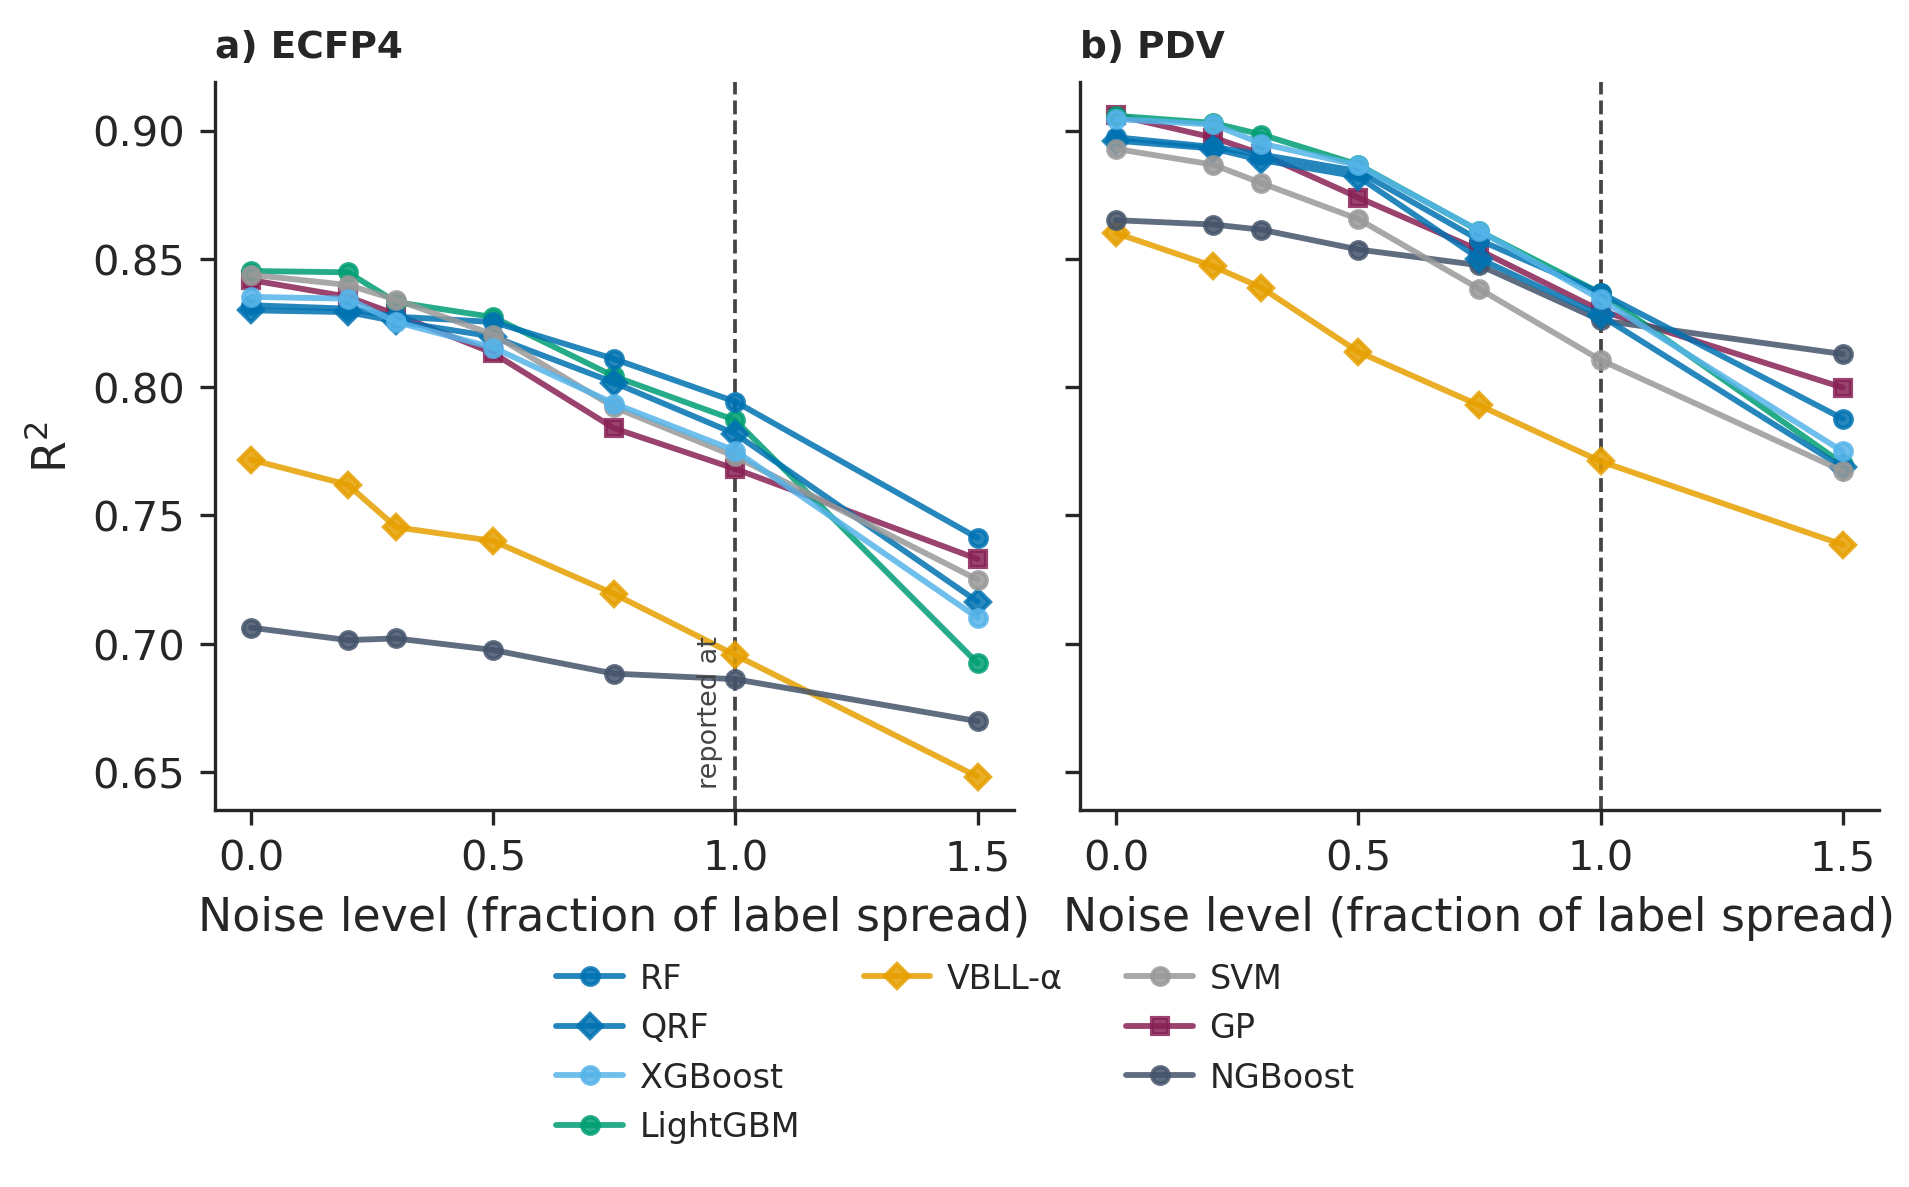
\includegraphics[width=\textwidth,height=0.72\textheight,keepaspectratio]{F4a_models_under_noise.png}
\caption[Predictive performance against Gaussian label noise on QM9.]{$R^2$ against noise level on the QM9 HOMO--LUMO gap under Gaussian noise, for the eight base models
with the highest \aucnorm{} on ECFP4: a) ECFP4; b) PDV. Medians over 10 replicates. The dashed line marks
the noise level of 1.0 at which $R^2$ is reported.}
\label{fig:curves}
\end{figure}

\begin{figure}[!htbp]
\centering
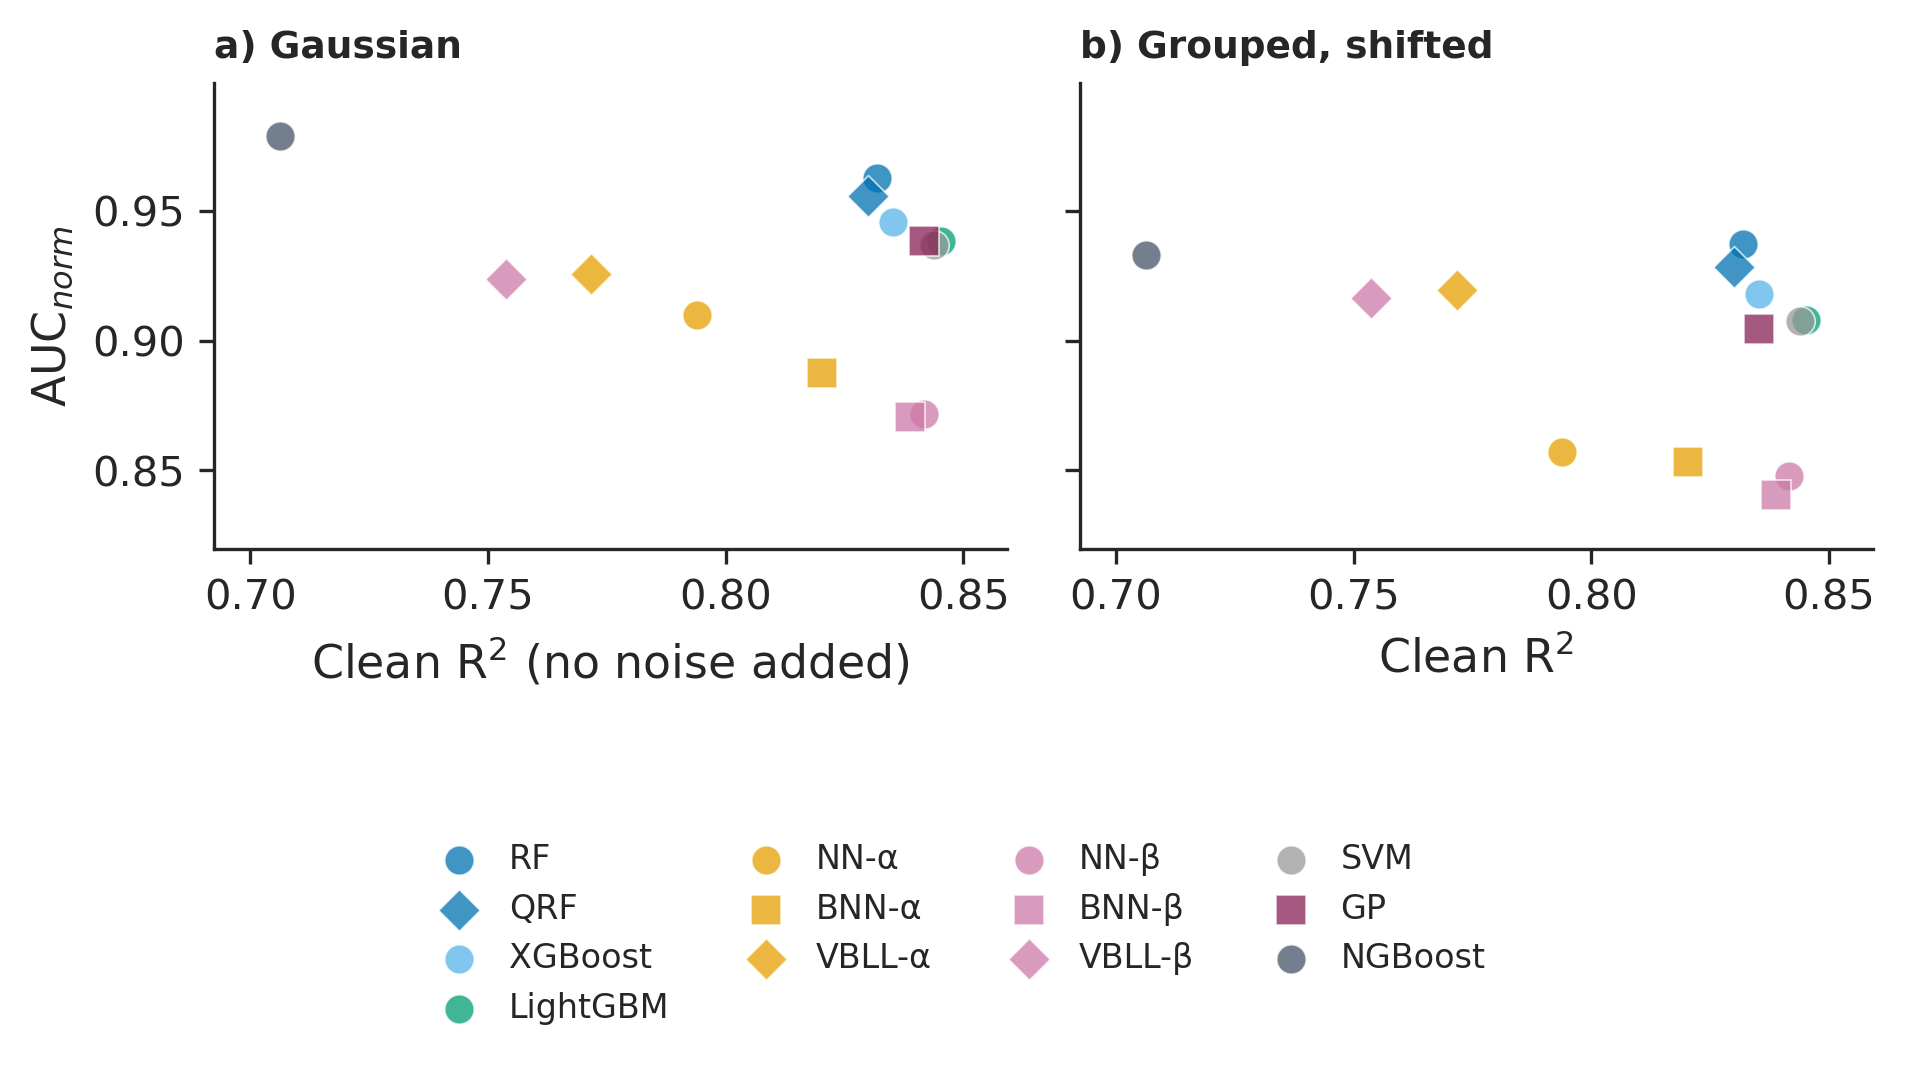
\includegraphics[width=\textwidth,height=0.72\textheight,keepaspectratio]{R16_decoupling_ecfp4.png}
\caption[Clean predictive performance against robustness on QM9.]{Clean $R^2$ against \aucnorm{} for each base model on the QM9 HOMO--LUMO gap with ECFP4, under
a) Gaussian and b) grouped-shifted noise.}
\label{fig:decoupling}
\end{figure}

\begin{figure}[!htbp]
\centering
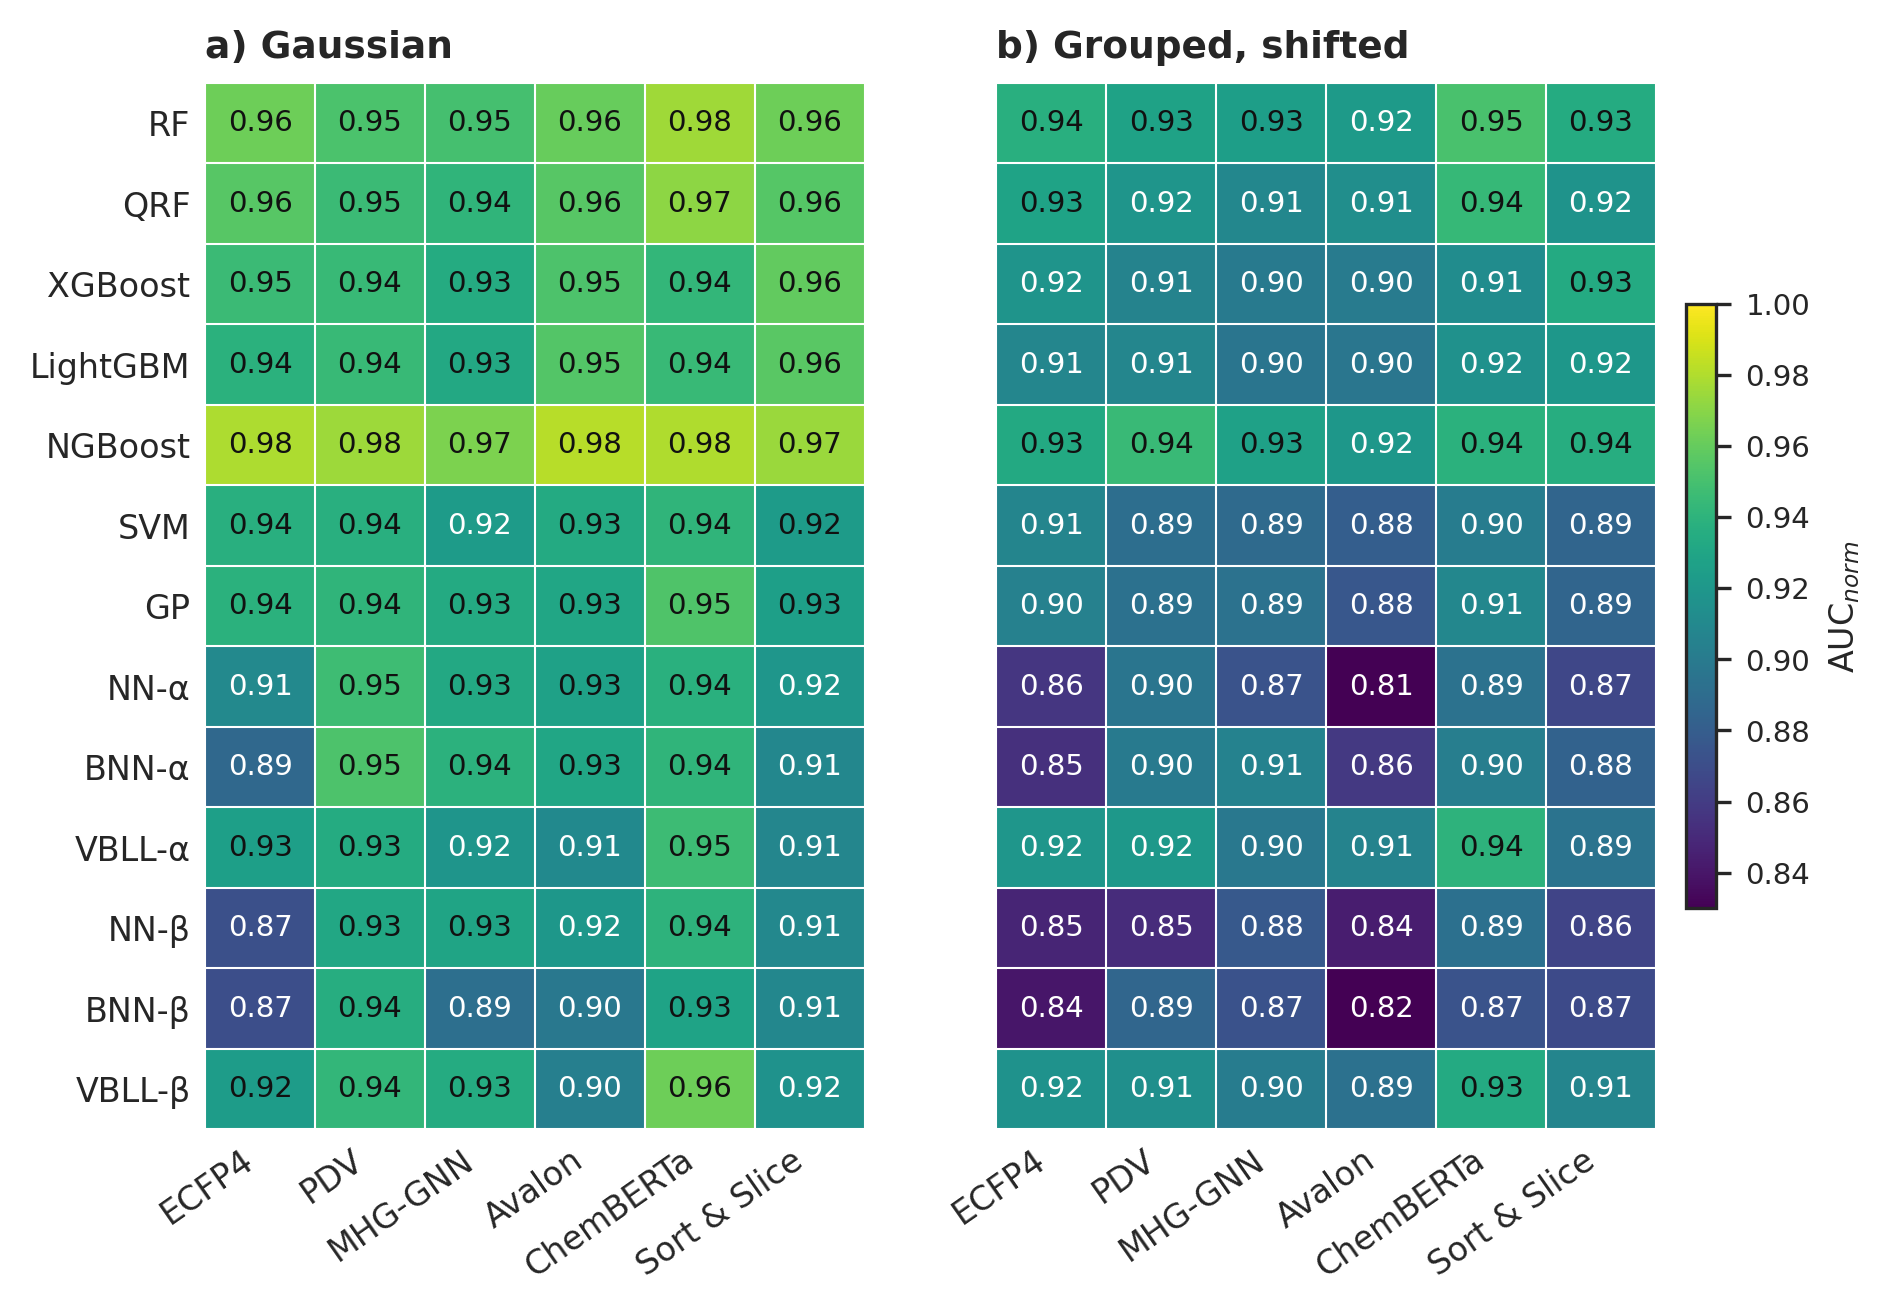
\includegraphics[width=\textwidth,height=0.72\textheight,keepaspectratio]{F3_model_by_representation.png}
\caption[Robustness of each base model on each representation on QM9.]{\aucnorm{} of the 13 base models on each representation, on the QM9 HOMO--LUMO gap under a) Gaussian
and b) grouped-shifted noise. Medians over 10 replicates, on one color scale. Excluded configurations are in
Additional file~\ref{app:noise:sec:excluded_configurations}; grouped-wider noise is in Additional file~\ref{app:noise:sec:grouped_wider_grid}.}
\label{fig:grid}
\end{figure}

\section{Artificial noise conditions}

Many studies involving experimental label noise rely on the assumption that noise can be modeled by a Gaussian distribution. We decided to vary the distribution which noise is drawn from, as well as the methodology by which it's injected to specific labels. Five of the seven conditions draw each label's error on its own, so the error is random. Grouped-shifted gives a whole scaffold family a shared offset, and censoring pulls every label above a limit down to that limit, so in both the error is systematic. We controlled the quantity of noise by adding it in proportion to the spread of the clean labels on the training set, so a difference between two conditions is a difference in pattern rather than amount. One condition, censoring, could not be held to a set amount as its levels count the fraction of labels clipped.

We compare Gaussian noise on the HOMO--LUMO gap to Laplace, Student-$t$ and outlier noise in Figure~\ref{fig:deep}. The shape of the distribution from which the noise was drawn from made little difference. SVM reported higher \aucnorm{} values on non-Gaussian label noise, 0.937 under Gaussian noise against 0.947, 0.952 and 0.955 under Student-$t$, outlier and Laplace noise on PDV, while NGBoost lost \aucnorm{} under every one. NGBoost's relative stronger performance on Gaussian makes sense as it fits a per-molecule scale under a Gaussian likelihood, which the other distributions violate. SVM gains \aucnorm{} and NGBoost loses it under all three distributions across all datasets and representations. The size of the shift stays small, which is why these results coincide with \citet{Heid2023}, who found no difference between error distributions drawn at a matched mean and standard deviation. The shape of the noise does not change how much performance a model keeps, but it does change which model keeps the most.

While alternative shapes of noise may be accurately modeled by the Gaussian distribution, we do not find that is the case for systematic label noise. Relative to Gaussian, grouped-shifted noise lowered the \aucnorm{} of across all models and representations (Table~\ref{tab:condition_cost}). The models struggle to make predictions when the noise is isolated on molecules of specific scaffold families instead of being applied randomly across every sample. The variational networks retained the most predictive performance, while the plain, deterministic NNs lost the most. The predictive abilities of BNN-$\alpha$ degraded at a slower rate compared to its deterministic counterpart on every representation except PDV, while BNN-$\beta$ did so only on MHG-GNN and PDV. Grouped-wider noise changed no model beyond its replicate spread except QRF on Avalon and MHG-GNN, which makes predictions particularly well under this noise condition.  Censoring created the largest drop in predictive performance, \aucnorm{} fell by 0.12 to 0.18 for the same QSAR models relative to Gaussian noise (Table~\ref{tab:censoring}).

Most of these observations are being made at the upper end of the noise range. With ECFP4, six of the seven most robust
models start within 0.015 of one another in $R^2$ for clean labels, stay together up to a noise level of 0.5 and
separate only above 1.0, finishing between 0.692 for LightGBM and 0.741 for RF
(Figure~\ref{fig:curves}). We ranked the models by predictive performance at each noise level. Of the 13 base models, RF started ranked seventh, but by level 1.0 it was ranked first. SVM on the other hand falls from first to fifth (Figure~\ref{fig:rank_level}). Because \aucnorm{} weights the whole range from 0 to 1.5 equally, and the first half of it separates little, it has the potential to understate just how much the pattern of the noise costs. However, choosing to look at performance of a set level has its drawbacks, as the ranks shift at a different pace between noise conditions.

\begin{figure}[!htbp]
\centering
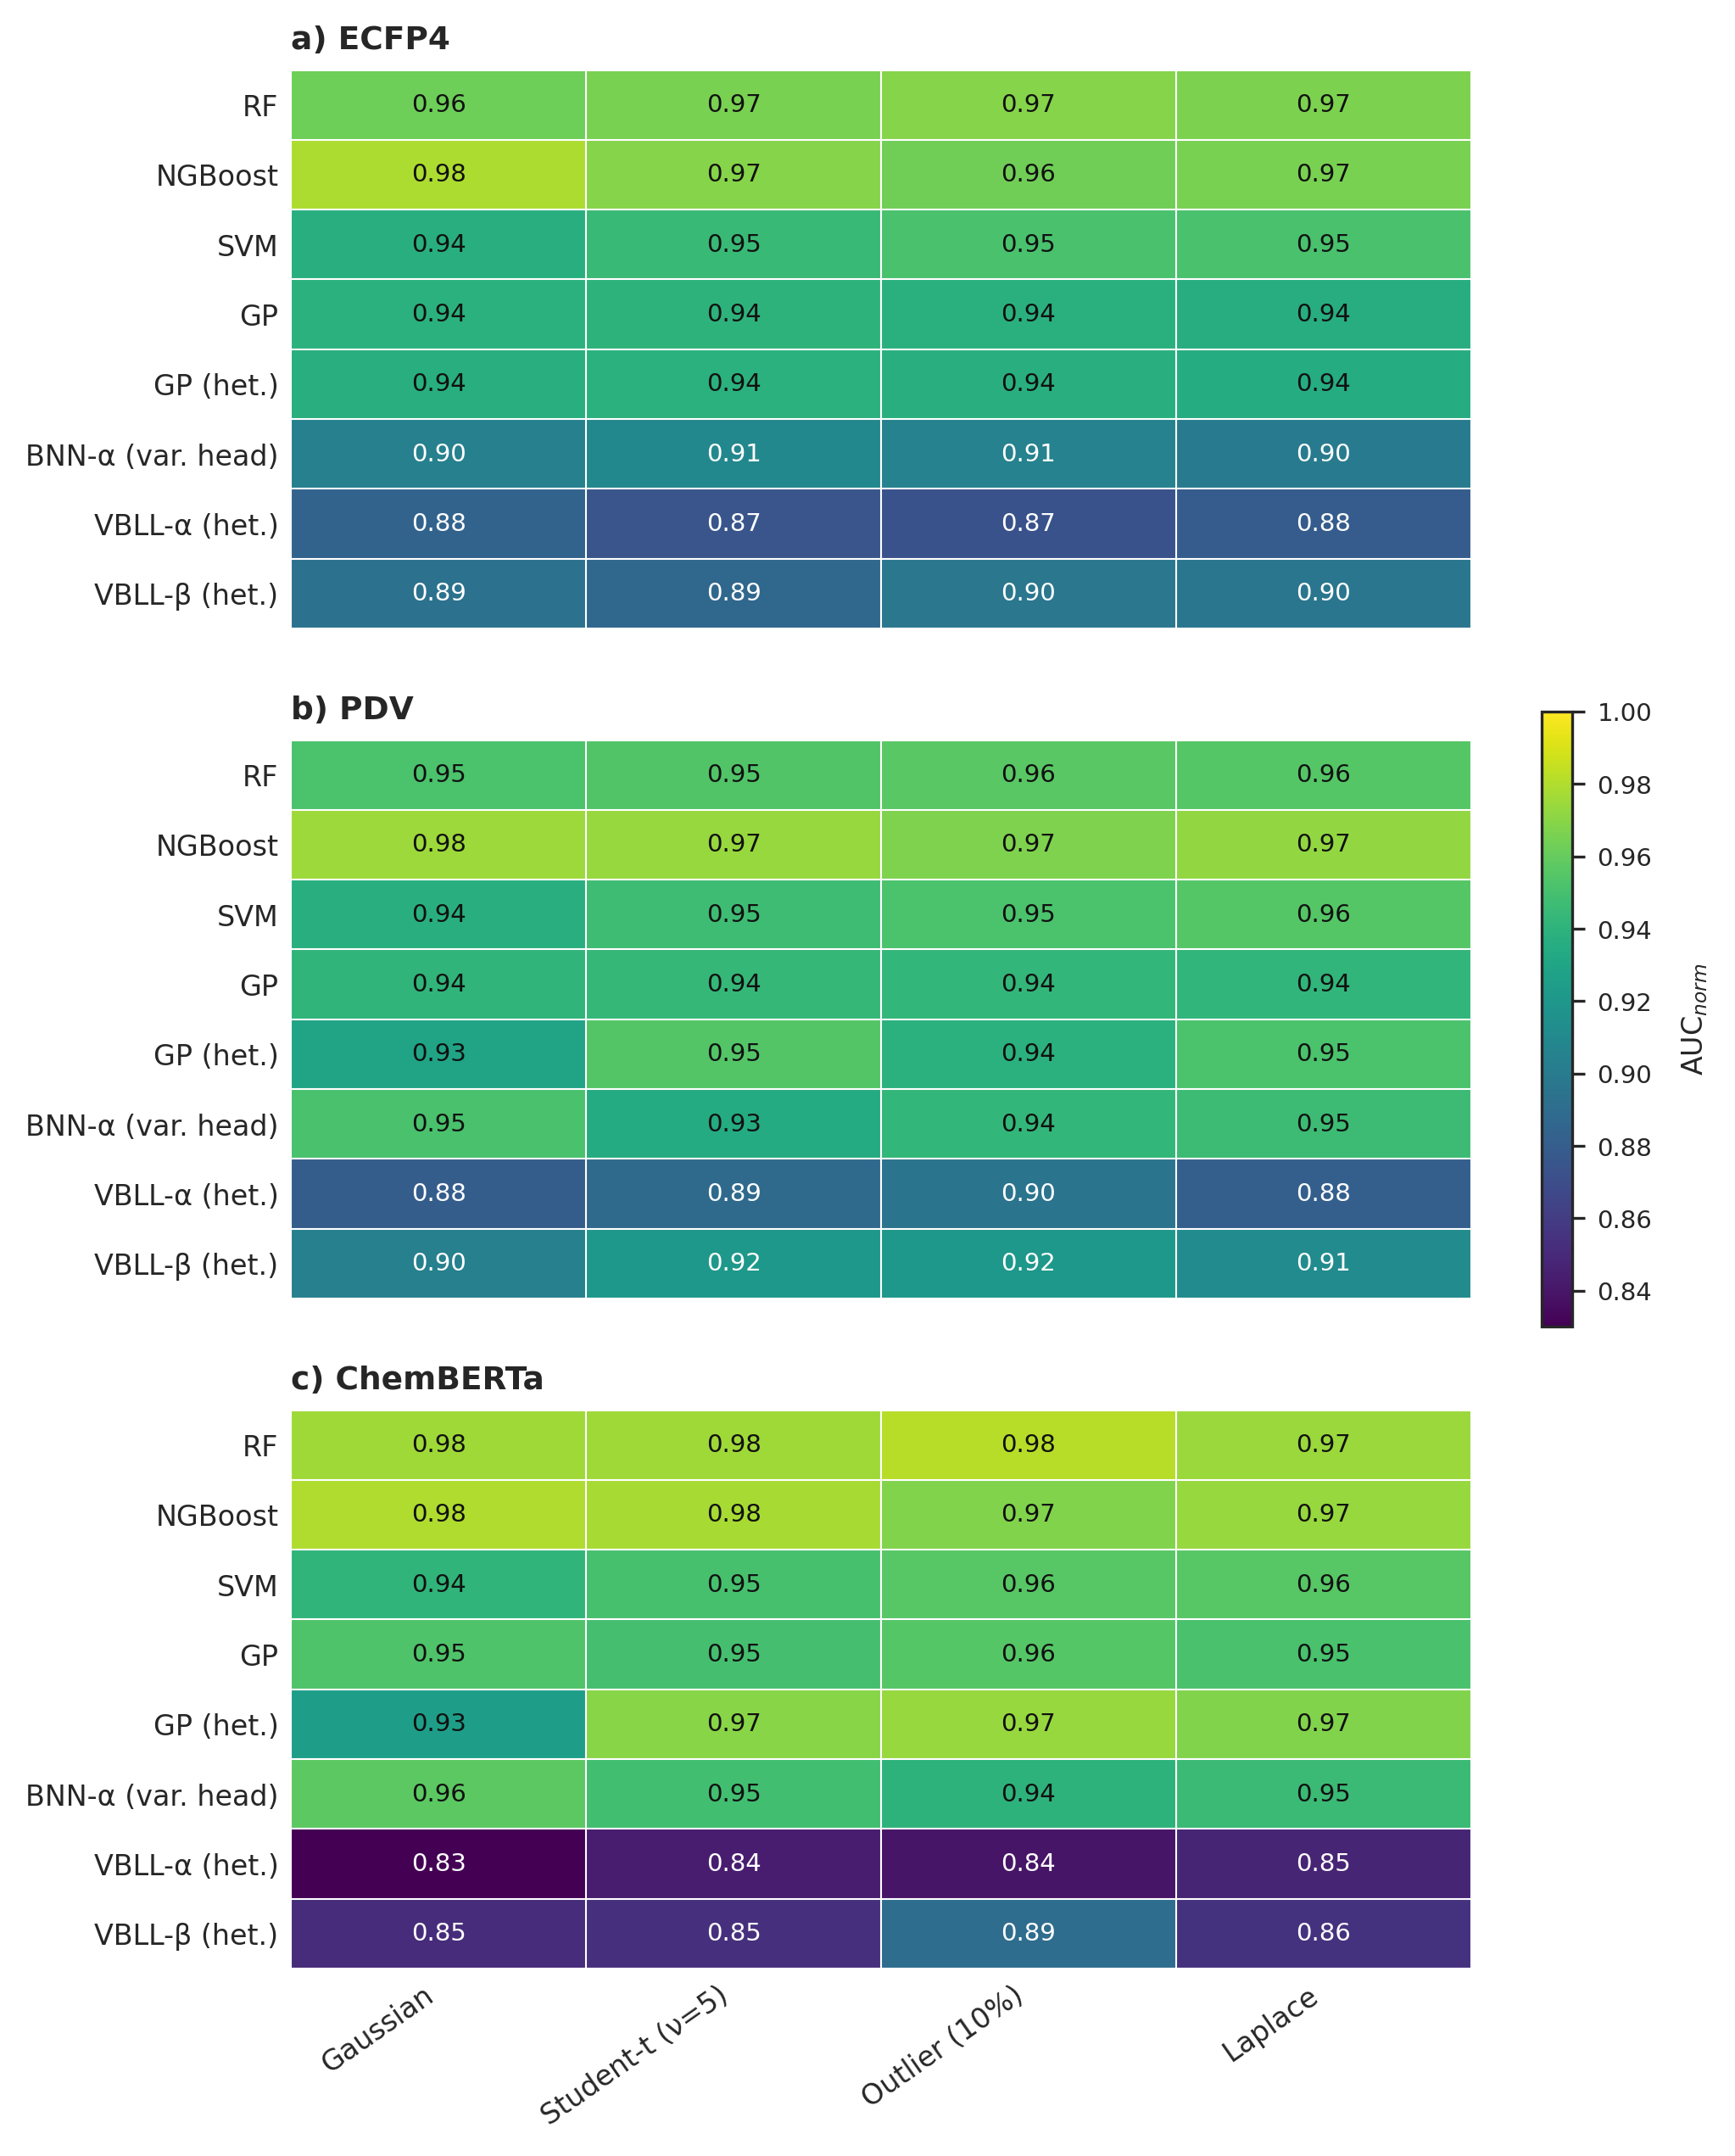
\includegraphics[width=\textwidth,height=0.72\textheight,keepaspectratio]{R19_deep_conditions_qm9.png}
\caption[Robustness under every noise condition on a subset of models on QM9.]{\aucnorm{} under the noise conditions run on a subset of models, on the QM9 HOMO--LUMO gap:
a) ECFP4; b) PDV; c) ChemBERTa. Medians over 10 replicates, on one color scale. Censoring is in
Table~\ref{tab:censoring}.}
\label{fig:deep}
\end{figure}

\begin{table}[!htbp]
\centering
\small
\begin{adjustbox}{max width=\textwidth,max totalheight=0.78\textheight}
\begin{tabular}{llccc}
\toprule
Model & Representation & Clean R$^2$ & Gaussian & Censoring \\
\midrule
RF & ECFP4 & 0.832 & 0.963 & 0.817 \\
GP (het.) & ECFP4 & 0.840 & 0.937 & 0.813 \\
NGBoost & PDV & 0.865 & 0.975 & 0.809 \\
GP & PDV & 0.906 & 0.941 & 0.815 \\
BNN-$\alpha$ (var. head) & PDV & 0.890 & 0.951 & 0.771 \\
\bottomrule
\end{tabular}
\end{adjustbox}
\caption[Robustness under censoring and under Gaussian noise on QM9.]{\aucnorm{} under censoring and under Gaussian noise on the QM9 HOMO--LUMO gap, for the five
model and representation pairs run under censoring. Medians over 10 replicates. A censoring level is the
fraction of labels clipped, so the two \aucnorm{} columns are on different scales.}
\label{tab:censoring}
\end{table}

\begin{table}[!htbp]
\centering
\small
\setlength{\tabcolsep}{3pt}
\begin{adjustbox}{max width=\textwidth,max totalheight=0.78\textheight}
\begin{tabular}{lccccccc}
\toprule
Model & ECFP4 & PDV & MHG-GNN & Avalon & ChemBERTa & \begin{tabular}[b]{@{}c@{}}Sort \&\\Slice\end{tabular} & \begin{tabular}[b]{@{}c@{}}Exceeds\\spread\end{tabular} \\
\midrule
RF & -0.025 & -0.024 & -0.025 & -0.038 & -0.025 & -0.028 & 6 of 6 \\
QRF & -0.027 & -0.027 & -0.032 & -0.042 & -0.027 & -0.038 & 5 of 6 \\
XGBoost & -0.028 & -0.039 & -0.035 & -0.052 & -0.030 & -0.025 & 5 of 6 \\
LightGBM & -0.030 & -0.037 & -0.037 & -0.058 & -0.028 & -0.037 & 5 of 6 \\
NGBoost & -0.046 & -0.030 & -0.039 & -0.062 & -0.041 & -0.039 & 6 of 6 \\
SVM & -0.029 & -0.045 & -0.034 & -0.053 & -0.040 & -0.038 & 5 of 6 \\
GP & -0.034 & -0.048 & -0.040 & -0.054 & -0.045 & -0.041 & 6 of 6 \\
NN-$\alpha$ & -0.053 & -0.051 & -0.060 & -0.115 & -0.044 & -0.053 & 4 of 6 \\
BNN-$\alpha$ & -0.034 & -0.053 & -0.034 & -0.073 & -0.039 & -0.025 & 2 of 6 \\
VBLL-$\alpha$ & -0.006 & -0.014 & -0.020 & -0.005 & -0.007 & -0.013 & 0 of 6 \\
NN-$\beta$ & -0.024 & -0.080 & -0.052 & -0.076 & -0.047 & -0.045 & 4 of 6 \\
BNN-$\beta$ & -0.030 & -0.050 & -0.019 & -0.075 & -0.055 & -0.041 & 2 of 6 \\
VBLL-$\beta$ & -0.007 & -0.028 & -0.033 & -0.010 & -0.028 & -0.009 & 0 of 6 \\
\bottomrule
\end{tabular}
\end{adjustbox}
\caption[Change in robustness from Gaussian to grouped-shifted noise on QM9.]{Change in \aucnorm{} from Gaussian to grouped-shifted noise on the QM9 HOMO--LUMO gap, per base
model and representation; negative is a loss. The last column counts the representations on which the loss exceeds the
replicate spread, the highest minus the lowest \aucnorm{} over 10 replicates under Gaussian noise.}
\label{tab:condition_cost}
\end{table}

\begin{figure}[!htbp]
\centering
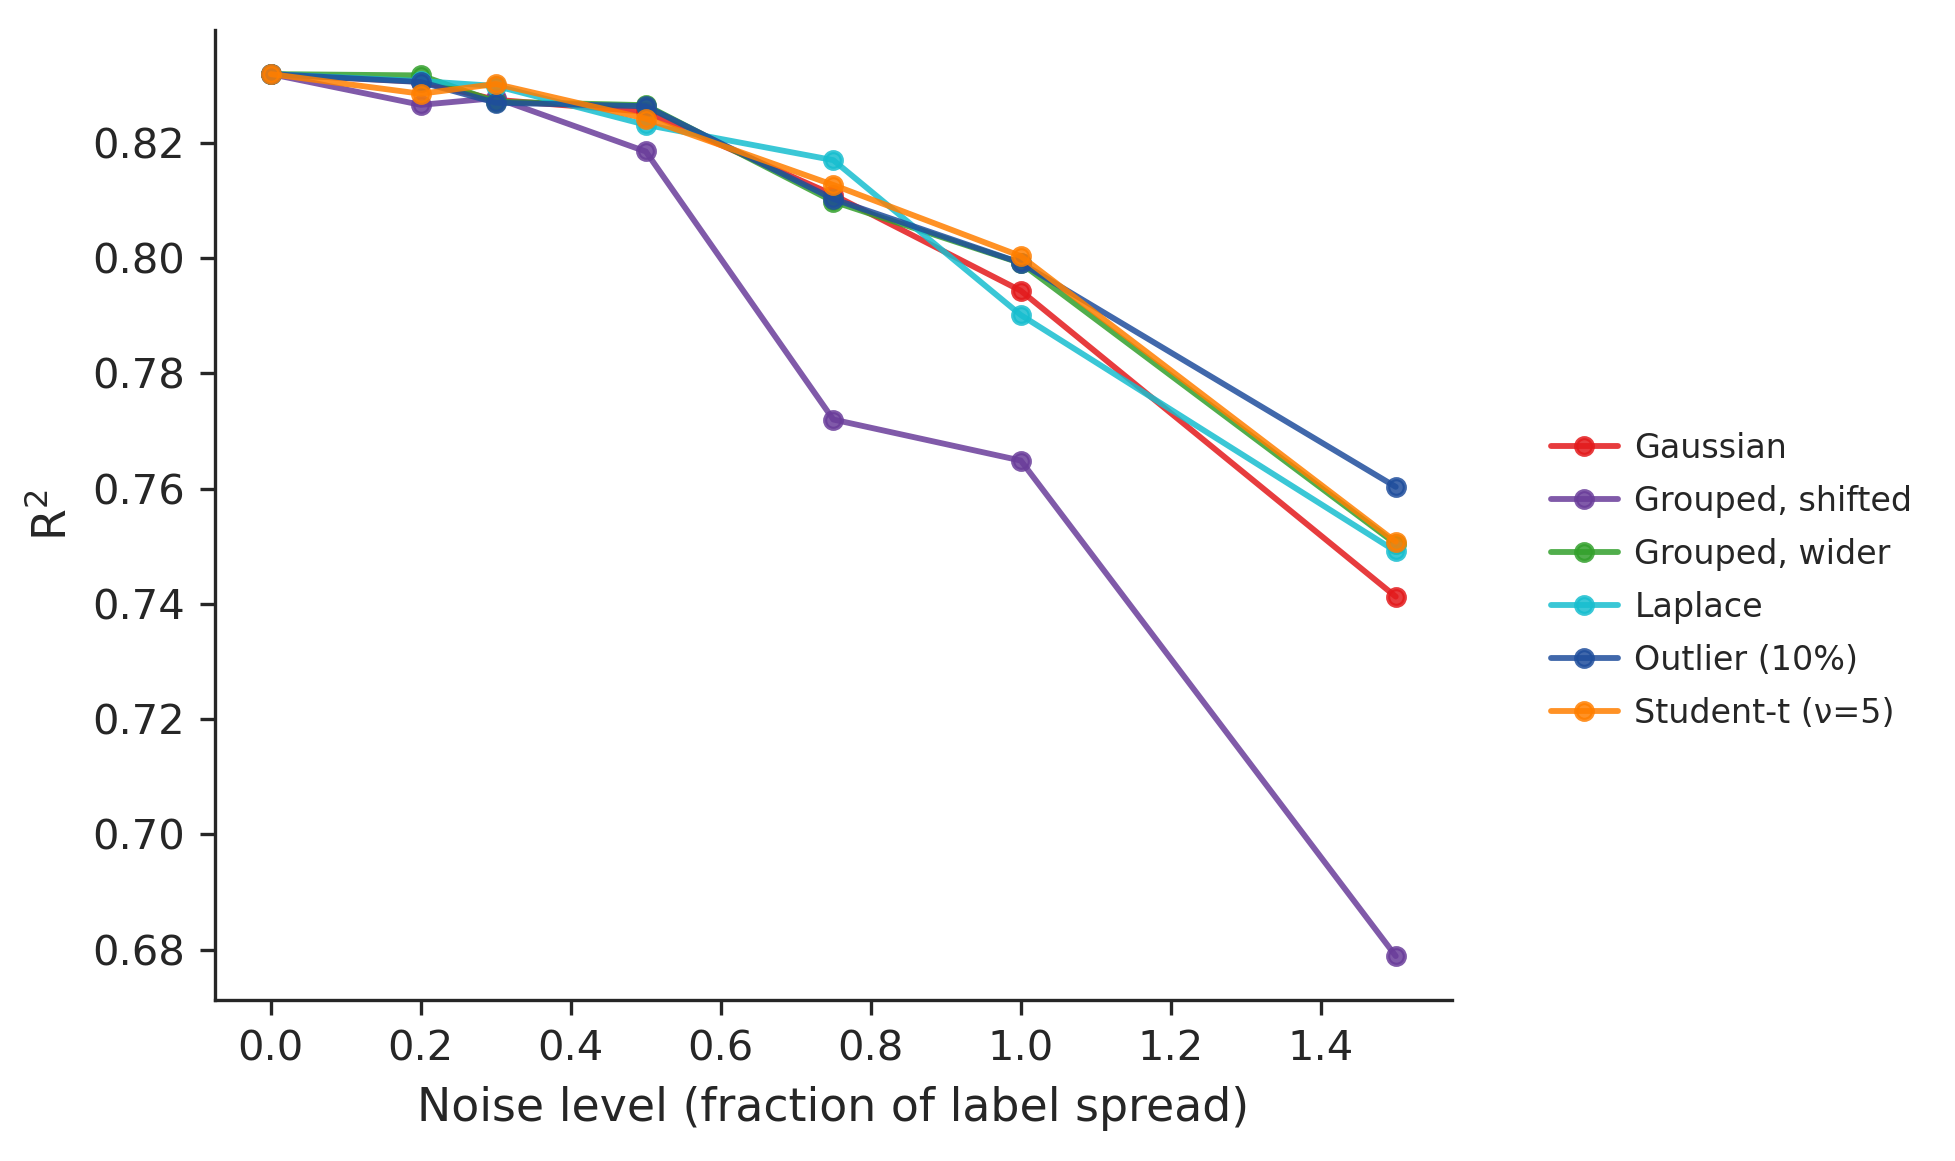
\includegraphics[width=\textwidth,height=0.72\textheight,keepaspectratio]{F4b_rf_across_noise_conditions.png}
\caption[Random forest under each noise condition on QM9.]{$R^2$ of the random forest against noise level under each noise condition, on the
QM9 HOMO--LUMO gap with ECFP4. Medians over 10 replicates. Censoring is not shown, as its level is a fraction of labels clipped.}
\label{fig:conditions}
\end{figure}

\begin{figure}[!htbp]
\centering
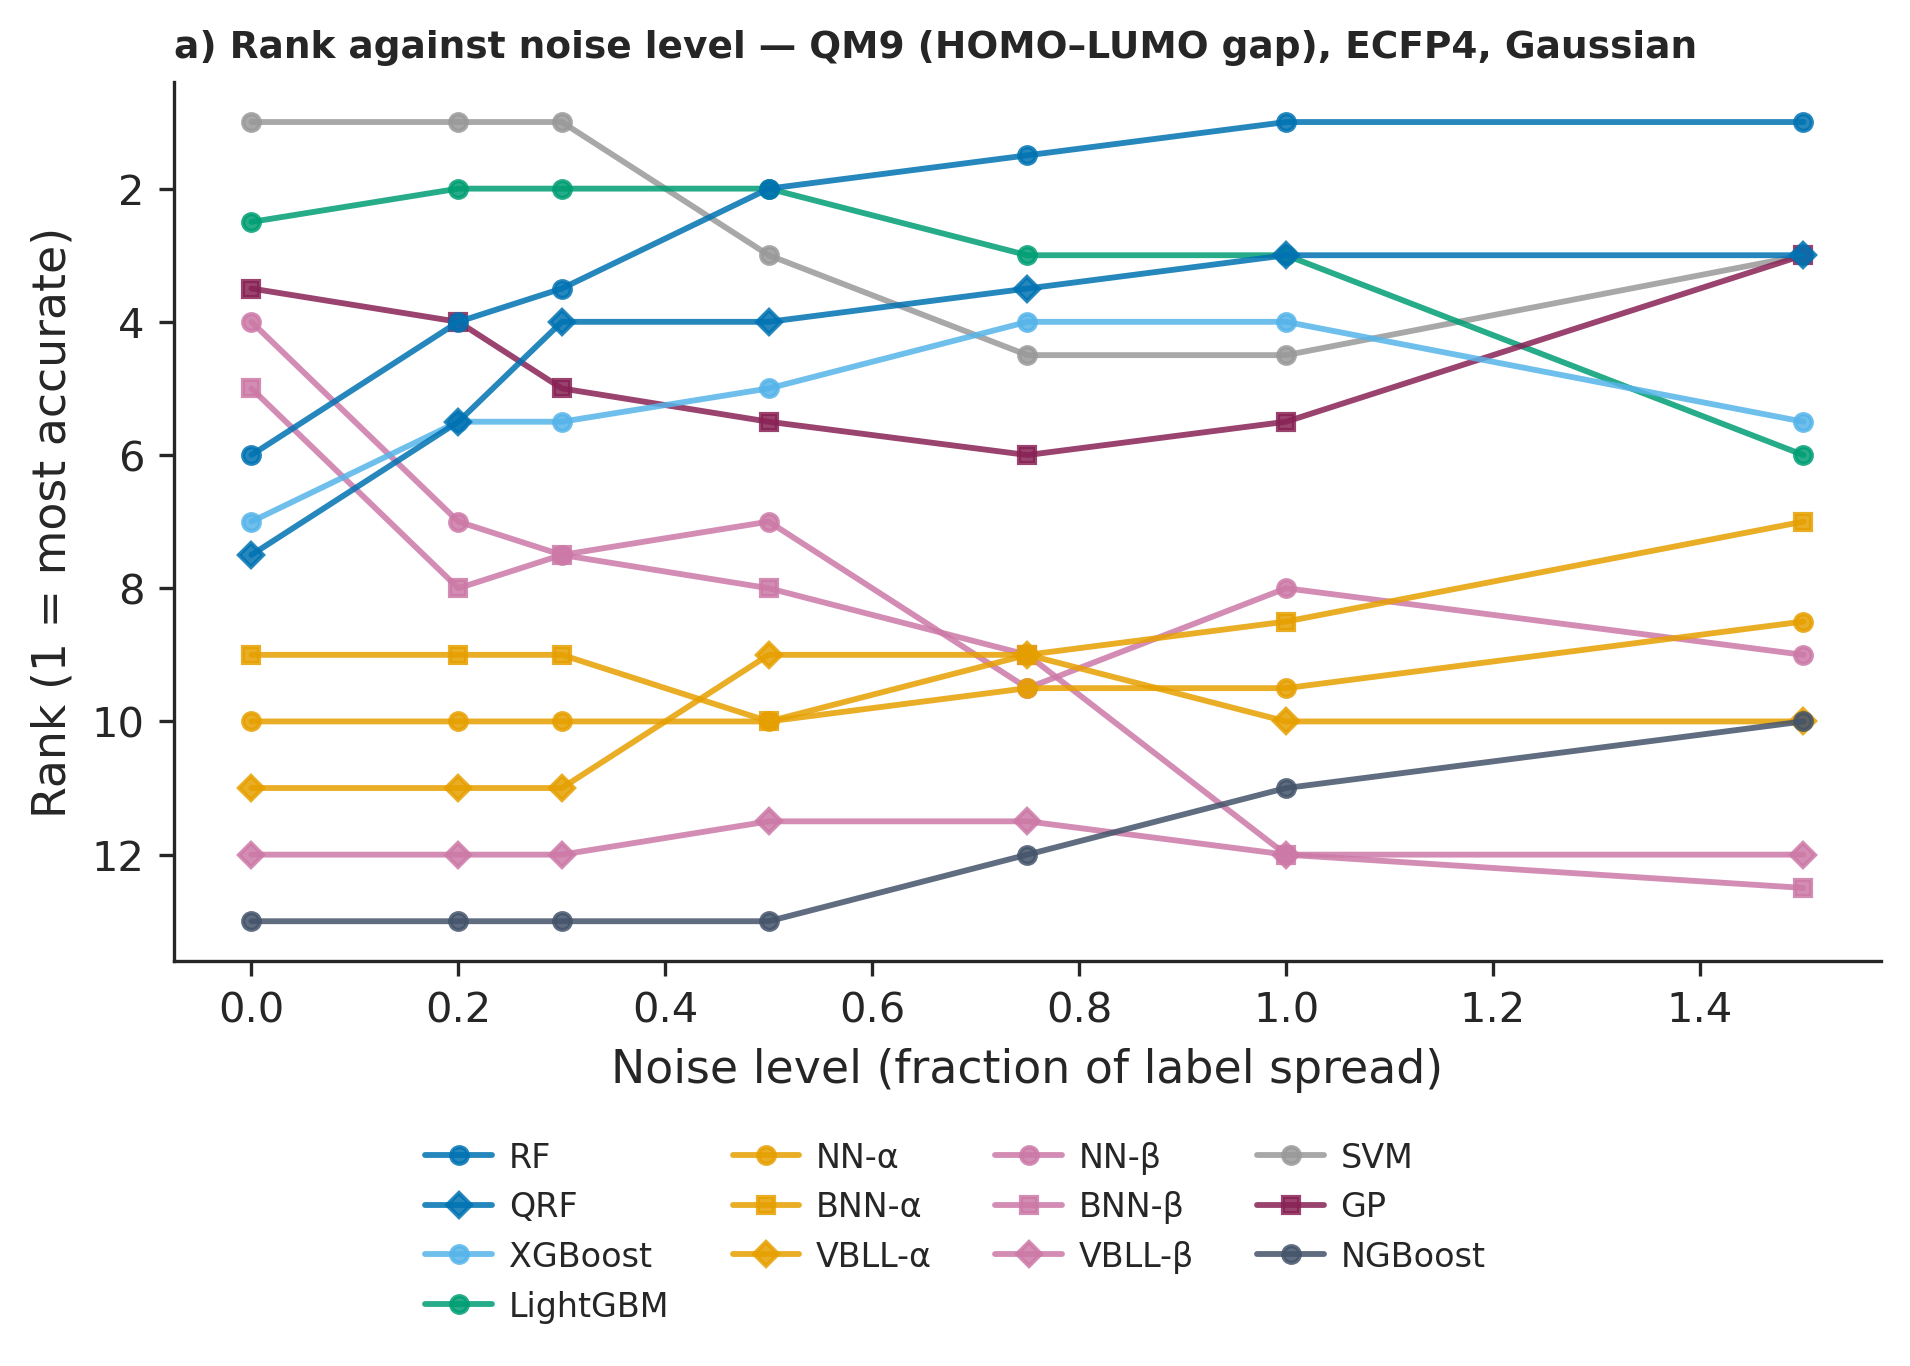
\includegraphics[width=\textwidth,height=0.36\textheight,keepaspectratio]{R15_rank_against_level_ecfp4_gaussian.png}\\[4pt]
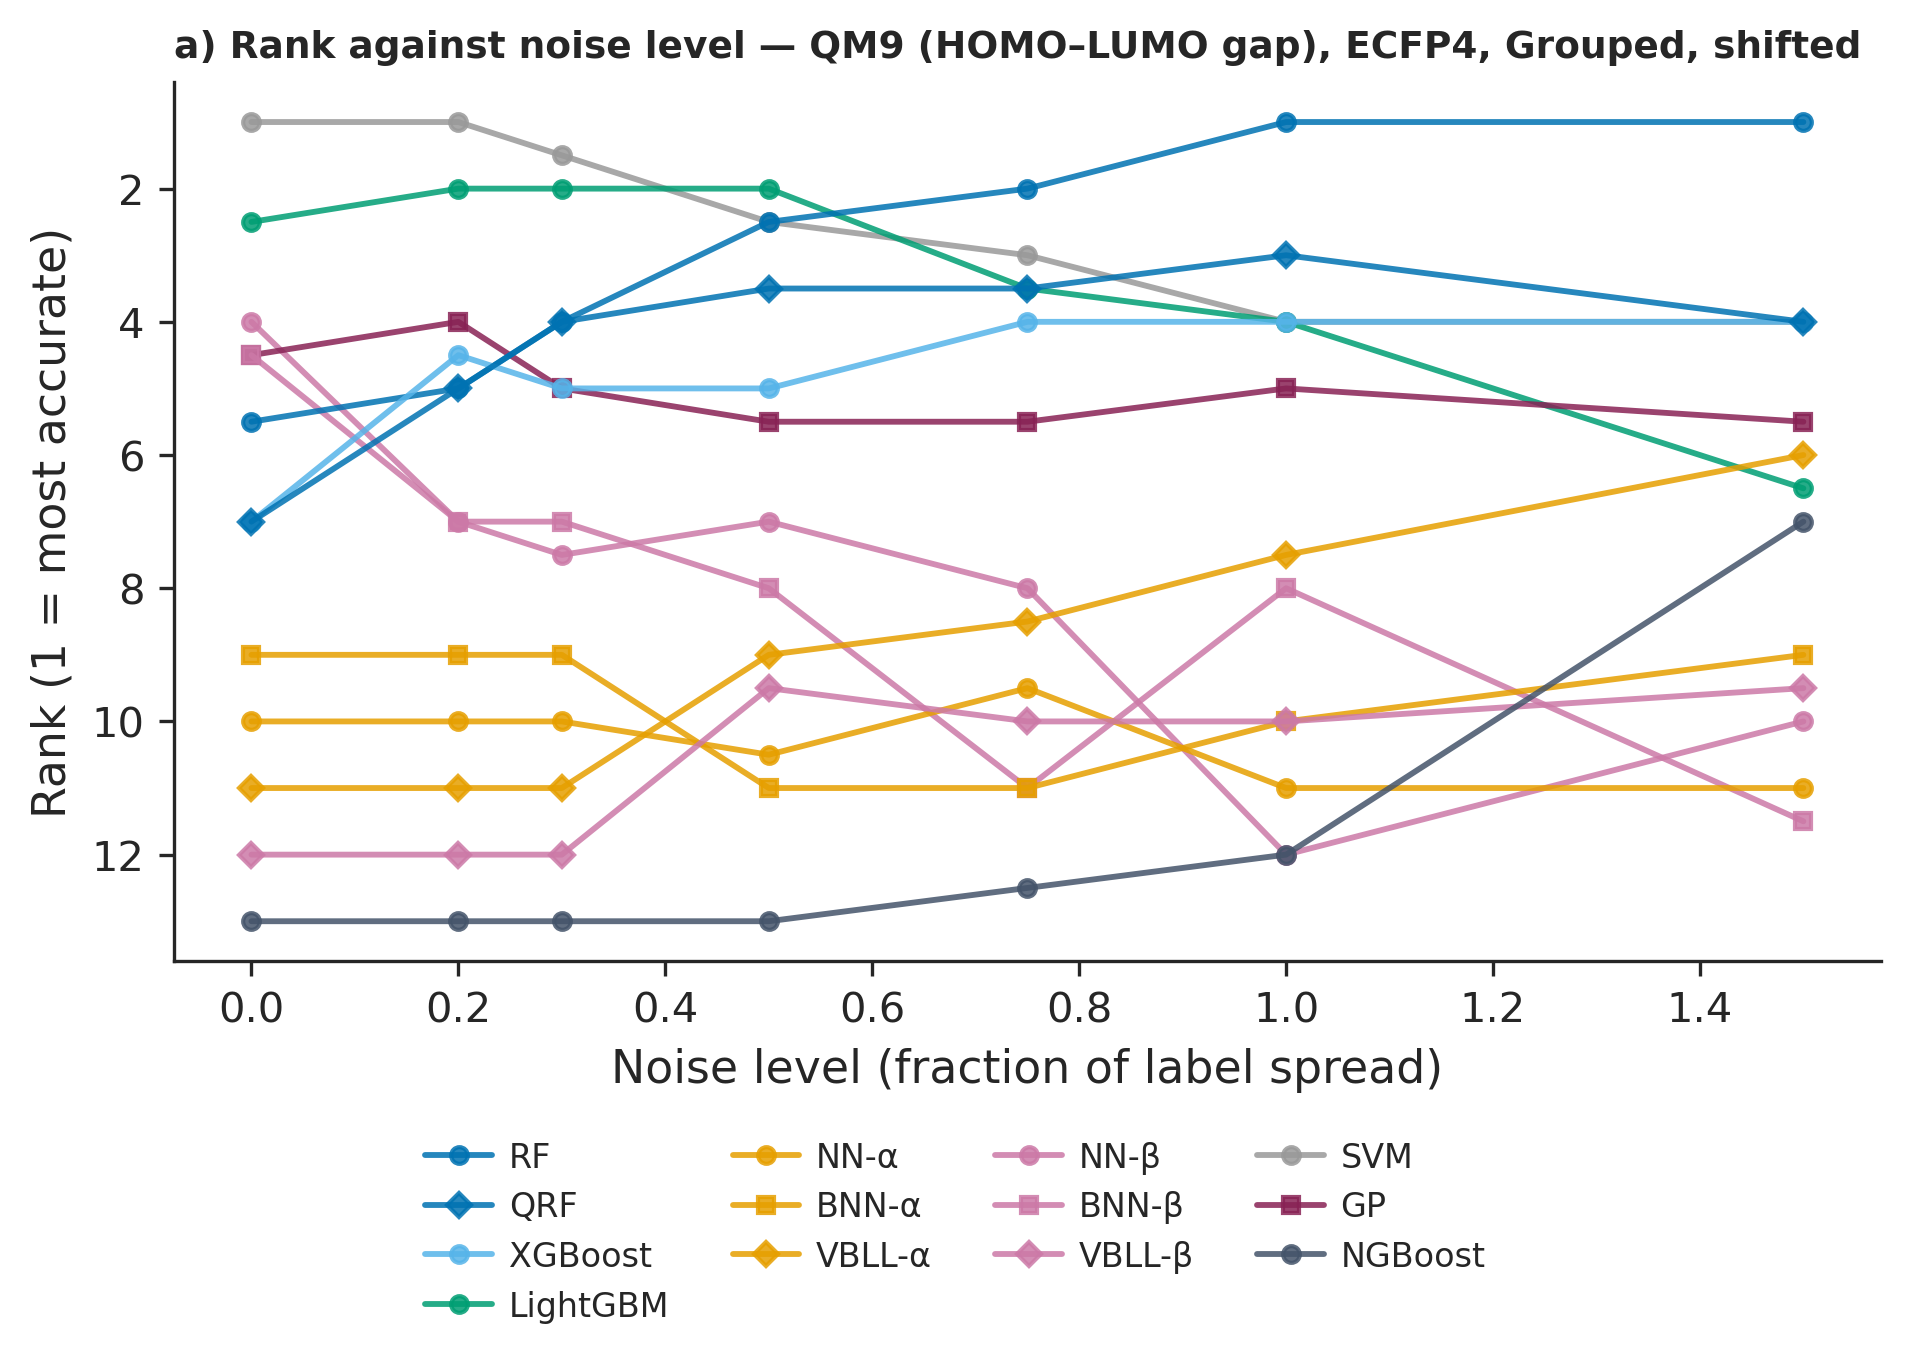
\includegraphics[width=\textwidth,height=0.36\textheight,keepaspectratio]{R15_rank_against_level_ecfp4_grouped_shifted.png}
\caption[Rank of each base model at each noise level on QM9.]{Median rank of each base model by $R^2$ at each noise level, on the QM9 HOMO--LUMO gap with ECFP4,
under a) Gaussian and b) grouped-shifted noise. Models are ranked within each replicate; tied medians give half ranks.}
\label{fig:rank_level}
\end{figure}

\section{Robustness on the three assay datasets}

So far, we have only discussed results coming on HOMO--LUMO gap from QM9, a computed property whose labels carry no measurement error. We repeated these experiments on three experimentally-obtained datasets,
LogD, Caco-2 \citep{openadmet}, and hERG $K_i$ \citep{Zdrazil2023}, replicating our process of adding artificial noise. Unlike QM9, the experimental endpoints carry their own measurement noise in both training and test labels; the injected artificial noise therefore adds on top of an unknown noise floor. Repeat measurements of the same compound disagree by about 0.54 log units for pK$_i$ \citep{Kalliokoski2013, Kramer2012}. The hERG $K_i$ labels have a spread of 0.915 log units, so a noise level of 0.6 of that spread is about one unit of that estimated laboratory error. Each model's \aucnorm{} under each noise condition on the three endpoints is given with its clean R$^2$ beside it (Figure~\ref{fig:assay}).

As on QM9, the noise distribution does not change the predictive capabilities of a model (Table~\ref{tab:assay_shape}). Laplace, Student-$t$ and outlier noise were run on seven models, RF, the two GPs, SVM, NGBoost, BNN-$\alpha$ (var. head) and VBLL-$\beta$ (het.), on ECFP4, PDV and ChemBERTa. Each delta below is measured from the same model's \aucnorm{} under Gaussian noise. RF and the two GPs never lose
more than 0.03 of \aucnorm{} under these three conditions or under grouped-wider noise, on any dataset or representation. SVM and NGBoost again move in opposite directions, SVM never loses \aucnorm{} under any of the four, while NGBoost loses under all four on Caco-2 and hERG $K_i$. The two networks move furthest in both directions. It's worth remembering that while we are injecting artificial noise, the assay measurements carry their own source of noise whose properties are unknown, so no ``clean'' label is truly clean.

\begin{table}[!htbp]
\centering
\small
\begin{adjustbox}{max width=\textwidth,max totalheight=0.78\textheight}
\begin{tabular}{lcccccc}
\toprule
Dataset & Model & Gaussian & Laplace & \begin{tabular}[b]{@{}c@{}}Student-t\\($\nu$=5)\end{tabular} & \begin{tabular}[b]{@{}c@{}}Outlier\\(10\%)\end{tabular} & \begin{tabular}[b]{@{}c@{}}Grouped,\\wider\end{tabular} \\
\midrule
logD & RF & 0.935 & +0.018 & +0.006 & +0.007 & +0.021 \\
logD & NGBoost & 0.924 & 0.000 & -0.028 & -0.032 & -0.009 \\
logD & SVM & 0.879 & +0.044 & +0.023 & +0.027 & +0.044 \\
logD & GP & 0.891 & +0.004 & +0.003 & -0.001 & +0.006 \\
logD & GP (het.) & 0.896 & 0.000 & -0.002 & -0.007 & -0.003 \\
logD & BNN-$\alpha$ (var. head) & 0.881 & -0.013 & -0.013 & -0.024 & -0.029 \\
logD & VBLL-$\beta$ (het.) & 0.796 & +0.010 & +0.012 & +0.020 & +0.068 \\
Caco-2 & RF & 0.865 & +0.035 & +0.028 & +0.026 & +0.053 \\
Caco-2 & NGBoost & 0.878 & -0.069 & -0.038 & -0.060 & -0.147 \\
Caco-2 & SVM & 0.841 & +0.049 & +0.051 & +0.031 & +0.018 \\
Caco-2 & GP & 0.809 & +0.039 & +0.034 & +0.020 & +0.023 \\
Caco-2 & GP (het.) & 0.815 & +0.035 & +0.032 & +0.011 & +0.019 \\
Caco-2 & BNN-$\alpha$ (var. head) & 0.787 & -0.110 & +0.092 & -0.043 & -0.017 \\
Caco-2 & VBLL-$\beta$ (het.) & 0.707 & +0.036 & +0.025 & +0.015 & +0.032 \\
hERG K$_i$ & RF & 0.898 & +0.015 & -0.006 & +0.016 & -0.012 \\
hERG K$_i$ & NGBoost & 0.842 & -0.031 & -0.027 & -0.042 & -0.093 \\
hERG K$_i$ & SVM & 0.859 & +0.051 & +0.035 & +0.025 & +0.055 \\
hERG K$_i$ & GP & 0.831 & +0.022 & +0.034 & +0.025 & +0.030 \\
hERG K$_i$ & GP (het.) & 0.843 & +0.010 & +0.036 & +0.015 & +0.021 \\
hERG K$_i$ & BNN-$\alpha$ (var. head) & 0.809 & -0.034 & -0.032 & -0.063 & -0.009 \\
hERG K$_i$ & VBLL-$\beta$ (het.) & 0.836 & +0.007 & -0.047 & +0.005 & -0.002 \\
\bottomrule
\end{tabular}
\end{adjustbox}
\caption[Robustness under the noise distributions on the three assay datasets.]{\aucnorm{} under Gaussian noise, and its change under each other noise condition, for a subset of models on the three assay datasets with ECFP4; negative is a loss. Medians over five scaffold folds.}
\label{tab:assay_shape}
\end{table}

Across all datasets, models struggle to fit with group-shifted noise the most, producing lower \aucnorm{} values across the board. For grouped-shifted, RF is the dominant model on hERG $K_i$ and logD, where it ranks first or second for \aucnorm{} with every representation. For predictive performance at under higher label noise (noise level 1.0), which is more impacted by the clean label performance, SVM ranks first to third on logD while RF ranks fifth to ninth across datasets. Both are strong contenders for systematic label noise.

LightGBM has particularly varied results across the datasets. On LogD, it has relatively high predictive performance and middle-of-the-pack noise robustness. However, on hERG and Caco-2, it loses the most with increased noise, particularly on Gaussian and grouped-shifted noise. The effects are not as pronounced on grouped-wider, although it still ranks among the least robust there.  XGBoost degrades in the same way on hERG and Caco-2.

While the results are not identical between the datasets, there are some patterns that emerge (Figure~\ref{fig:transfer}). In general, the relative \aucnorm{} model rankings match between QM9 and logD, as well as between Caco-2 and hERG $K_i$ with every representation except ChemBERTa.  RF is the most consistent, among the 13 base models under Gaussian noise it ranks between first and seventh for \aucnorm{} on every dataset and representation, second or third on QM9 and first on logD at five of six. The GP has the highest predictive performance on clean labels on all three assay datasets with nearly every representation, and ranks third to ninth for \aucnorm. NGBoost, the most robust model on QM9, ranks first to third on logD, second to tenth on Caco-2 and sixth to ninth on hERG $K_i$. LightGBM falls furthest, ranking 10th to 13th on Caco-2 and hERG $K_i$ at every representation while being among the highest in predictive performance on clean labels. VBLL-$\alpha$ is the opposite, ranking first or second for \aucnorm{} on hERG
$K_i$ and last on logD at every representation, from one of the lowest clean $R^2$ values. This fits the pattern of the NNs being exceptionally varied.

We consider the impact of label noise on each model family. While the forests, RF and QRF, are typically middle-ground in terms of predictive performance on clean labels, they are the most reliably robust to noise across all datasets. Their rank barely changes between noise conditions, so there is no pattern of noise they are better suited to. Caco-2 is the exception, where they rank third to seventh rather than first or second.

Other models perform conditionally well, and in some cases that condition is the representation they are paired with. The GP has some of the higher predictive capabilities on clean labels and under Gaussian noise across assay datasets. It is the highest on logD and Caco-2 under grouped-wider noise as well, but under grouped-shifted noise it falls. The choice of representation has little impact on GP, moving its \aucnorm{} less than repeating the split does on every dataset.

There is a slight consideration with using both \aucnorm{} and predictive performance side-by-side. \aucnorm{} measures the fraction of its own clean $R^2$ that a model keeps, so predictive performance on clean labels works against it by construction. A model that already predicts poorly has little to lose and often scores a higher \aucnorm, while a model that starts with strong performance has more to lose. The GP and NGBoost are the clearest cases. The GP has among the highest predictive performance on clean labels and a middling \aucnorm, while NGBoost has the highest \aucnorm{} across the board from one of the lowest clean $R^2$ values. While NGBoost's predictive performance is highly dependent on its representation, its robustness is not. On QM9 it is both the most robust model and the lowest ranked model for predictive performance up to a noise level of 0.75 with every representation. But with PDV it's able to retain some predictive performance under noise, finishing highest across all the models at noise level 1.5.

Upon first glance, SVM does not seem like a standout, however, it is the model whose standing is better with non-Gaussian noise. Among RF, the GP, NGBoost and SVM, the four models run under every condition, SVM has the lowest \aucnorm{} of the four under Gaussian noise on almost every dataset and representation, and rises to second under Laplace, Student-$t$ and outlier noise and under grouped-wider noise. Gaussian noise is actually the one condition it is worst at. Its \aucnorm{} stays in the middle, partially because it starts high, and it ranks among the five highest for predictive performance at a noise level on every assay dataset under every noise condition.

The feed-forward networks are the most variable, although in general they have some of the highest predictive performance under clean labels and are generally not robust to noise. They are also dependent on the choice of representation. VBLL networks perform poorly on clean labels, are the least robust to noise on logD, yet are the most robust on Caco-2 and hERG $K_i$. The gradient-boosted trees, LightGBM and XGBoost, were also quite variable, with strong predictive performance on clean labels and poor noise robustness on Caco-2 and hERG $K_i$.

The quantity of noise is an important factor as well. At a noise level of 0.5 the models still rank by predictive performance much as they do on clean labels, while by 1.0 the order has changed, most of all on hERG $K_i$ and then QM9. The order of models by \aucnorm{} is broadly similar across noise conditions, with the forests near the top under each.

While it is clear that QSAR model performance drops with label noise, different models drop faster than others. How much noise a dataset tolerates before anything happens is itself a property of the dataset. Up to a noise level of 0.3, three tenths of the spread of the clean labels, the models are largely unaffected by the noise on the HOMO--LUMO gap and on logD, where every base model with ECFP4 still keeps at least 93\% of its clean $R^2$; on Caco-2 one of the 13 and on hERG $K_i$ four of the 13 are already below 90\% at that level. By a noise level of 0.5 the lowest retained fraction is 90\% on the HOMO--LUMO gap against 76\% on hERG $K_i$ (Figure~\ref{fig:curves_all}). Boosted tree ensembles are some of the first to fall. On Caco-2 with ECFP4, LightGBM has among the highest predictive performance on clean labels. It is also the first tree ensemble to fall below 90\% of that performance, at a noise level of 0.5. By level 1.5 it retains 26\% of its original $R^2$, compared to 63\% for RF on ECFP4. XGBoost drops off at the next recorded noise level. However, NGBoost is the opposite, having some of the lowest predictive performance on clean labels and the flattest curve with injected label noise across all models. On the HOMO--LUMO gap it never falls below 90\% of its clean $R^2$ at any level tested. The networks drop at an inconsistent rate. VBLL-$\alpha$ is the earliest to fall on logD, dropping below 90\% of its clean $R^2$ at a level of 0.5 and reaching 38\% by 1.5. Yet on Caco-2 and hERG $K_i$ it is among the flattest models.

\begin{figure}[!htbp]
\centering
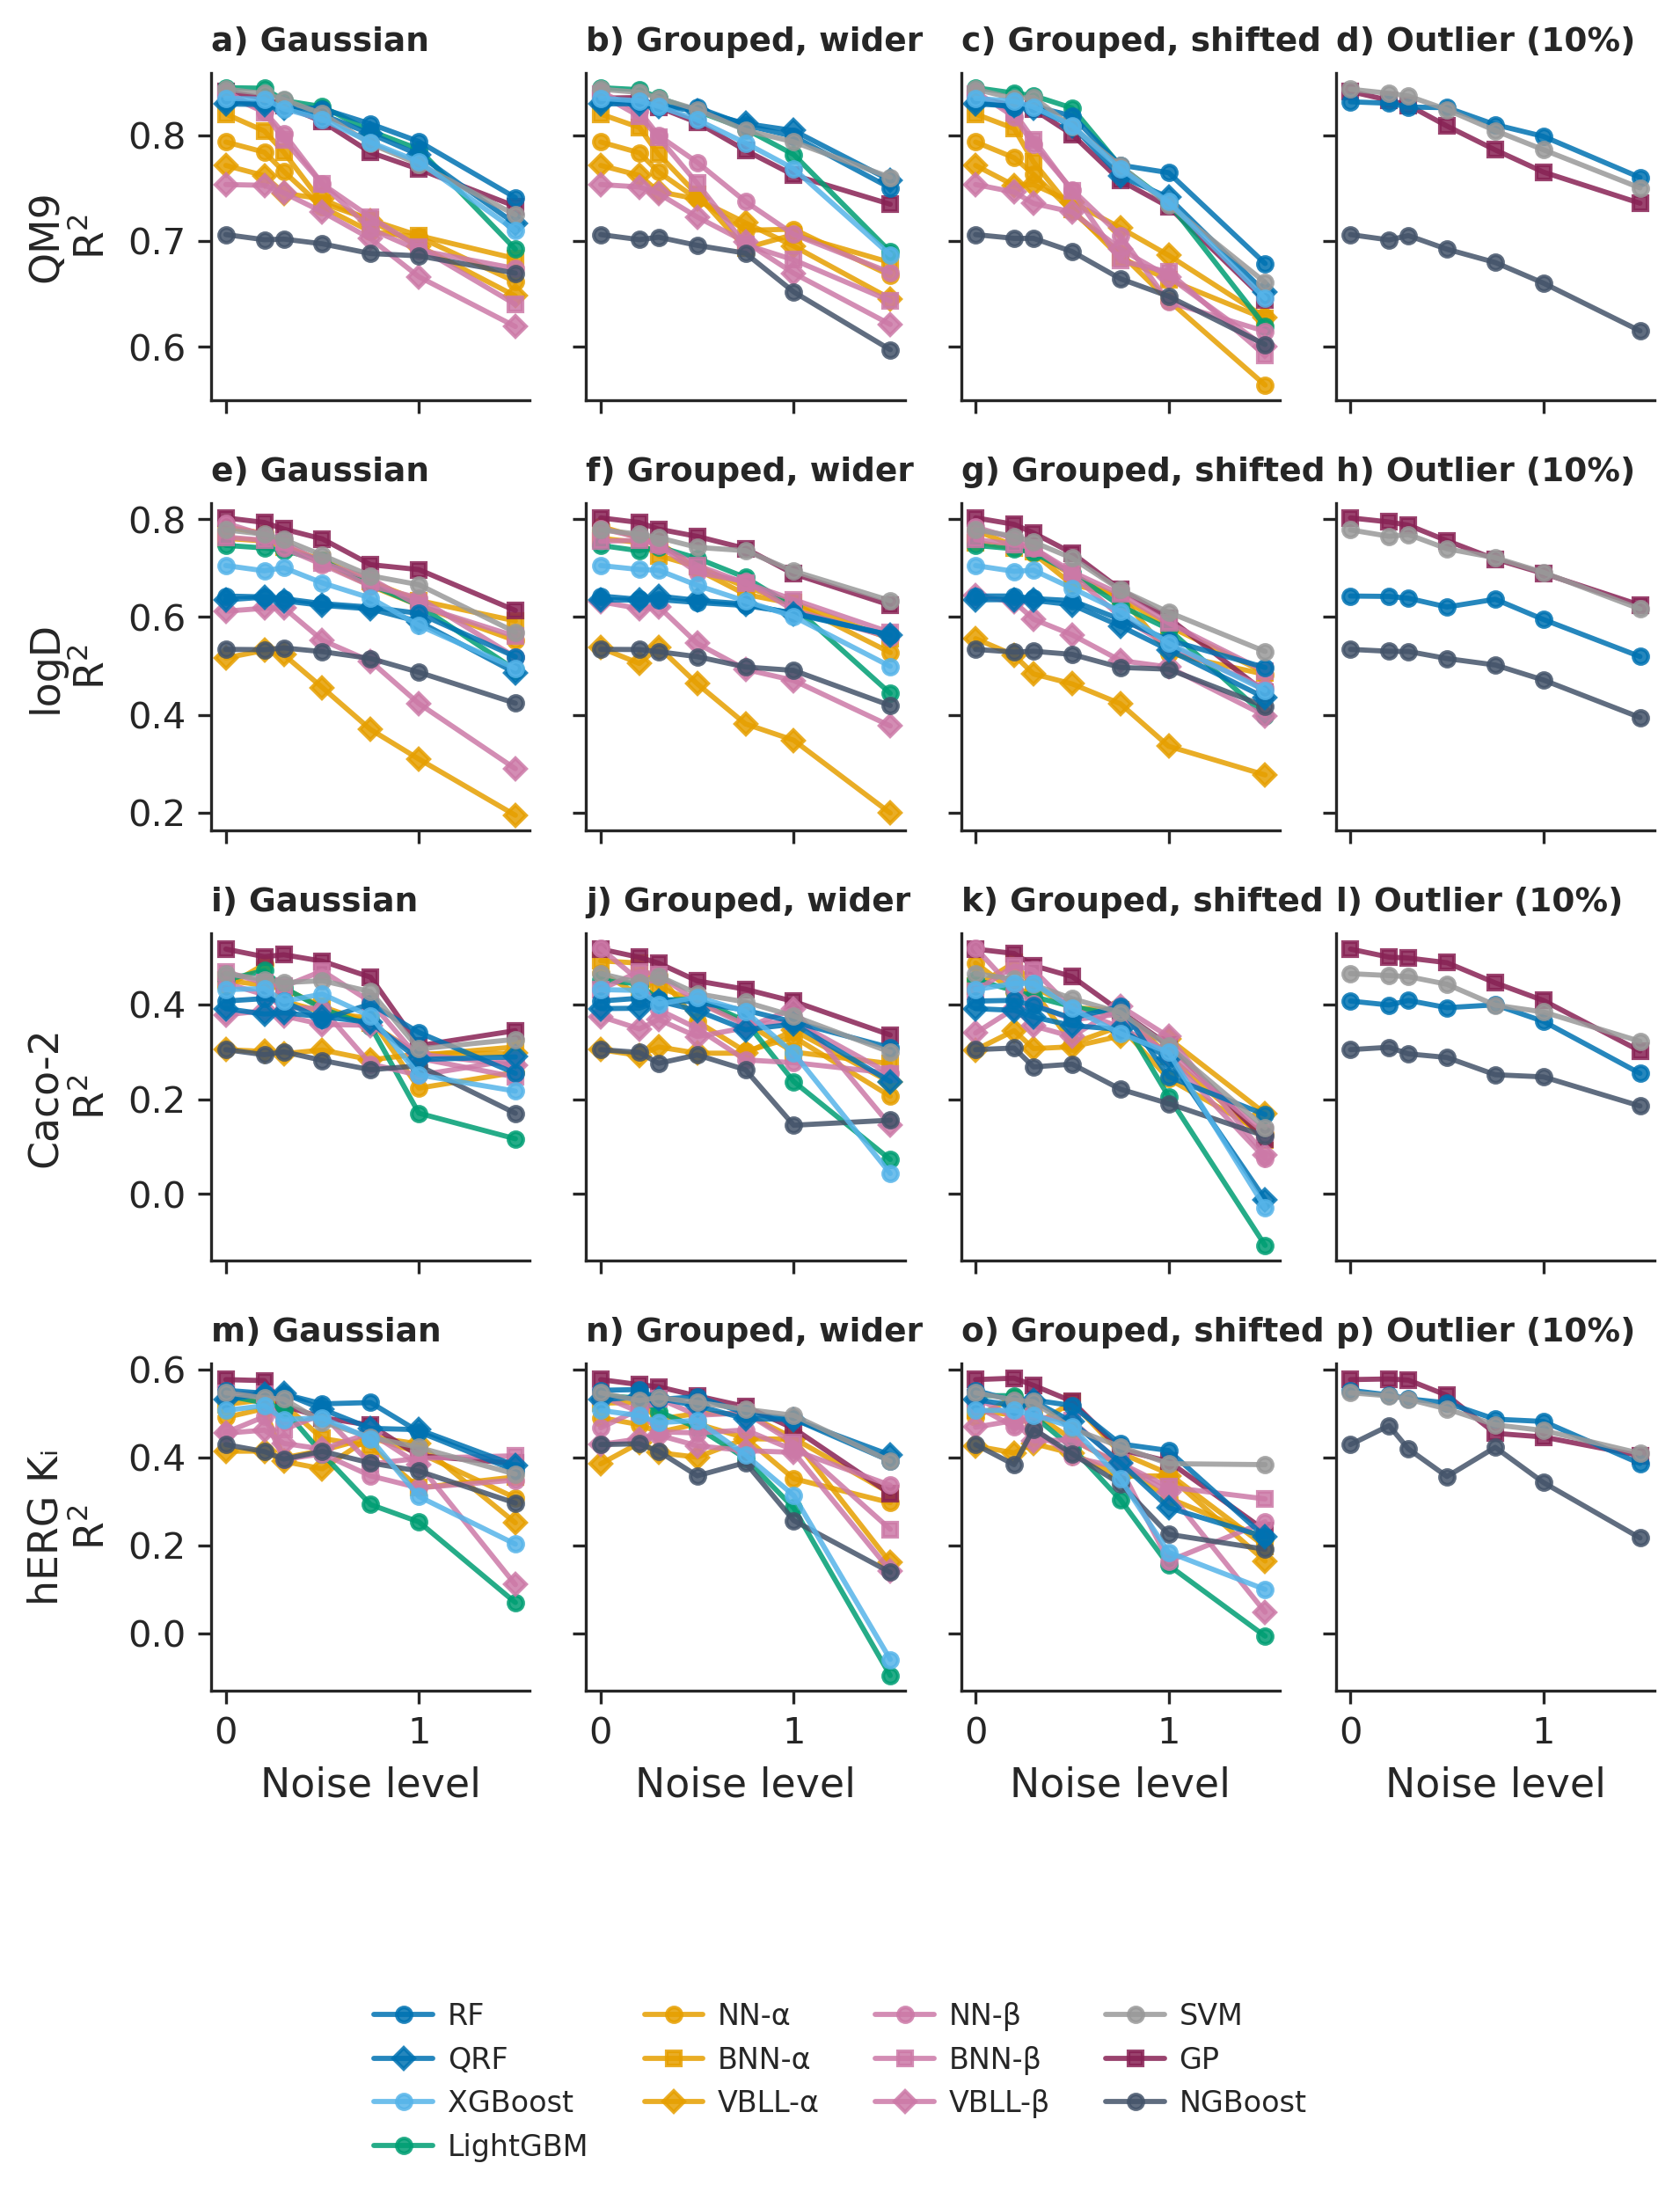
\includegraphics[width=\textwidth,height=0.72\textheight,keepaspectratio]{F8c_curves_every_dataset_ecfp4.png}
\caption[Predictive performance against noise level on every dataset.]{$R^2$ against noise level for the 13 base models on every dataset with ECFP4. Rows are
datasets and columns noise conditions: a)--d) QM9 HOMO--LUMO gap; e)--h) logD; i)--l) Caco-2; m)--p) hERG $K_i$.
Medians over 10 replicates on QM9 and five scaffold folds on the assay datasets.}
\label{fig:curves_all}
\end{figure}

\begin{figure}[!htbp]
\centering
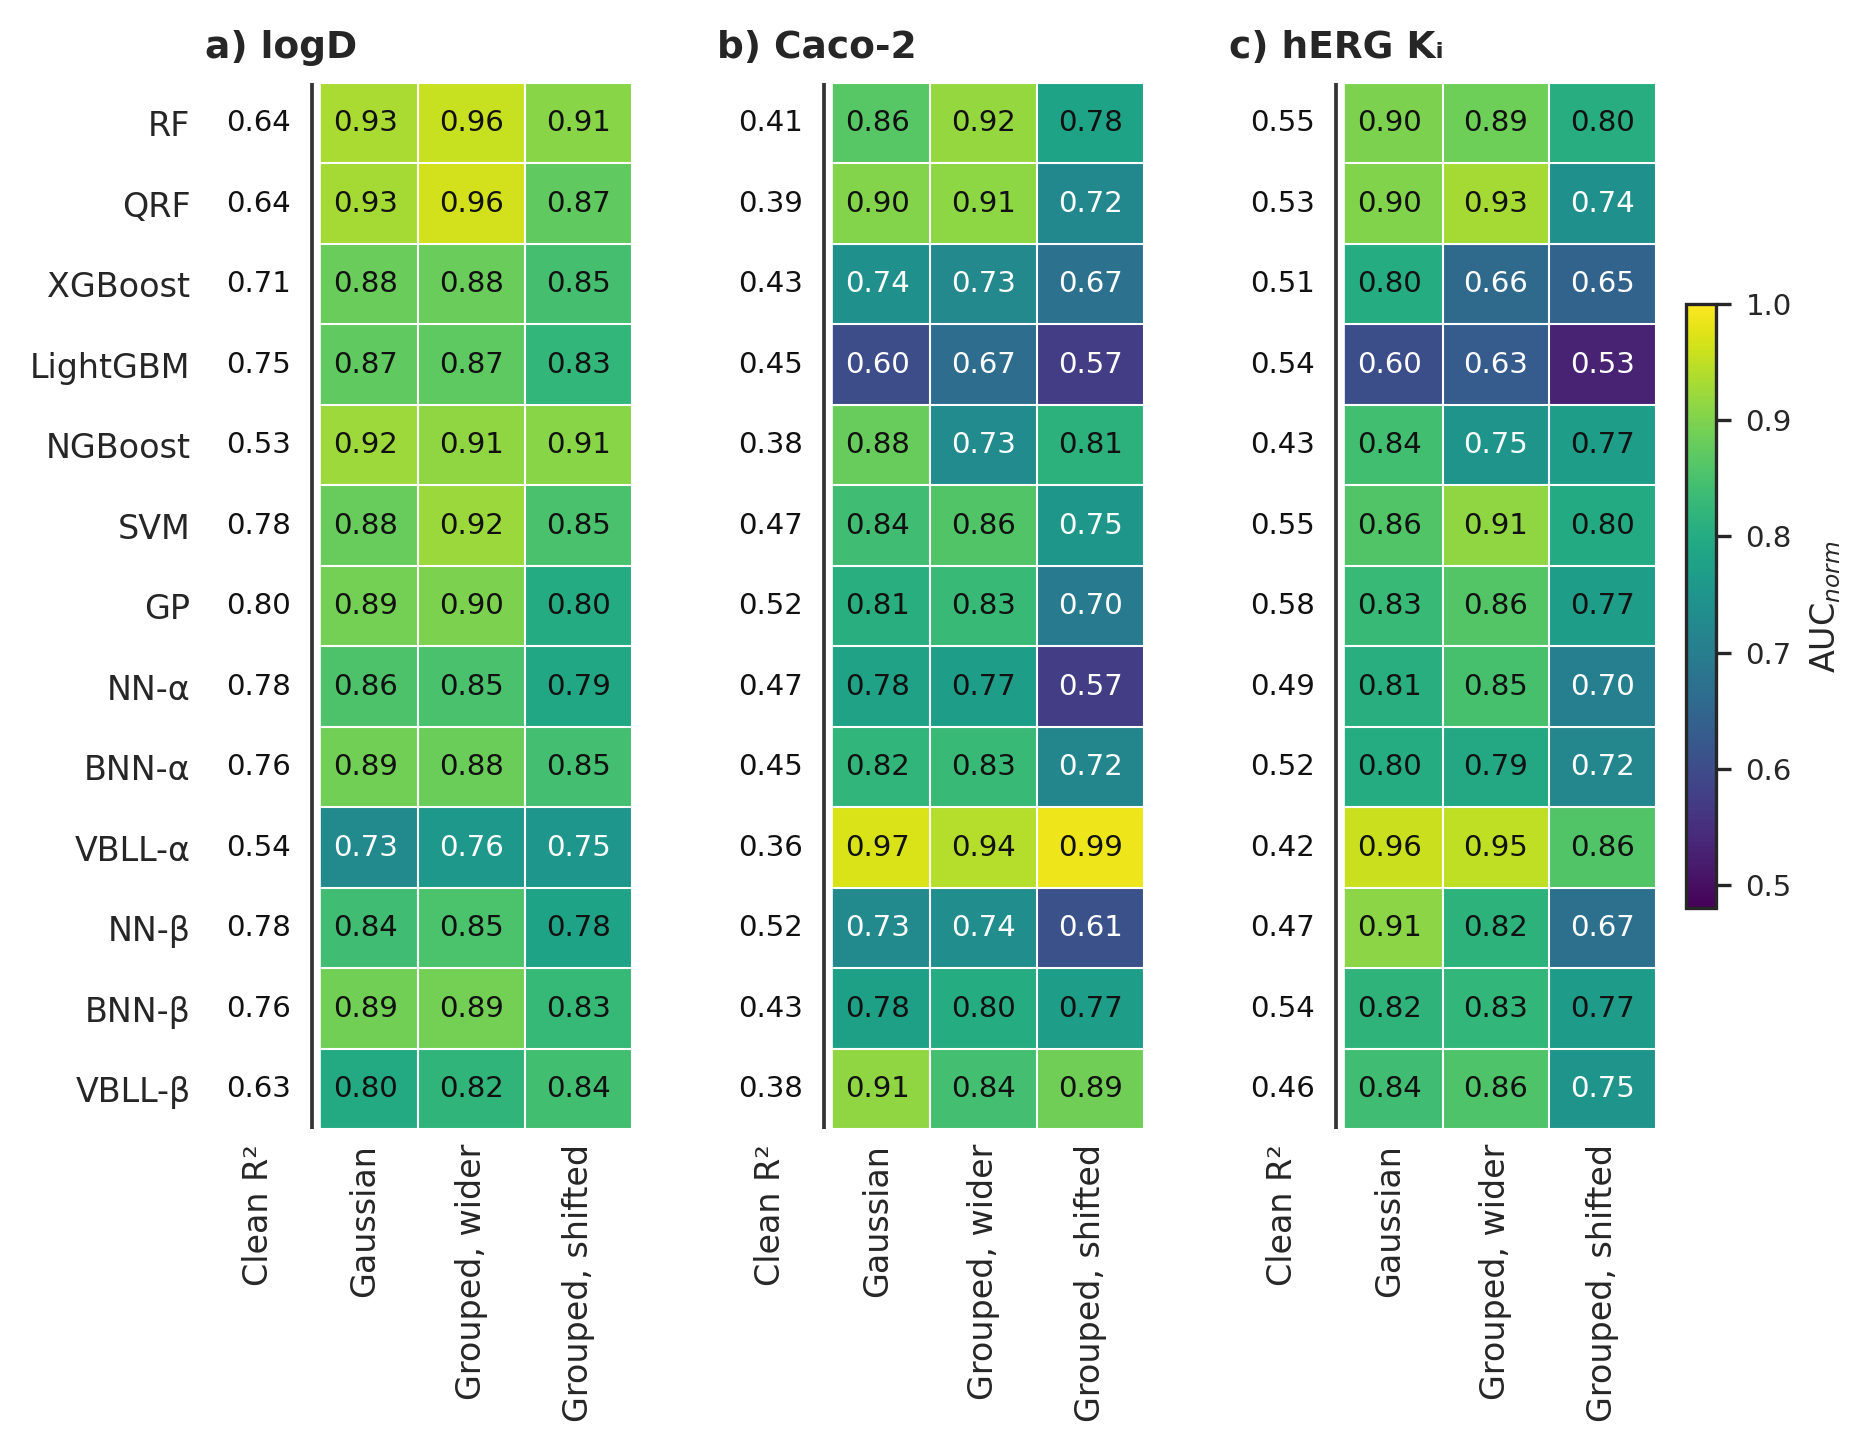
\includegraphics[width=\textwidth,height=0.72\textheight,keepaspectratio]{F8_assay_datasets.png}
\caption[Robustness on the three assay datasets.]{\aucnorm{} of the 13 base models with ECFP4 on a) logD, b) Caco-2 and c) hERG $K_i$,
under the three noise conditions run on every model. The first column is clean $R^2$. Medians over the
scaffold folds that pass the clean-$R^2$ threshold (Additional file~\ref{app:noise:sec:excluded_configurations}), on one color scale. The variant
models are in Additional file~\ref{app:noise:sec:variant_models_assay}.}
\label{fig:assay}
\end{figure}

The variance decomposition of predictive performance tells us how much the choice of model and representation matters under clean labels (Figure~\ref{fig:three_outcomes}; Additional file~\ref{app:noise:sec:variance_intervals}). Extending that concept, we are also interested how these shares change under increasing label noise and compare to the variance decomposition of \aucnorm. The replicate and residuals account for more variance across all datasets. On Caco-2 and hERG $K_i$ the replicate, which on these datasets is one of five scaffold folds, is the largest share of predictive performance before and after noise is injected. Conversely, it falls well below the choice model family for robustness. On every dataset the interaction between model and representation explains more of the variance in \aucnorm{} than representation alone.

\begin{figure}[!htbp]
\centering
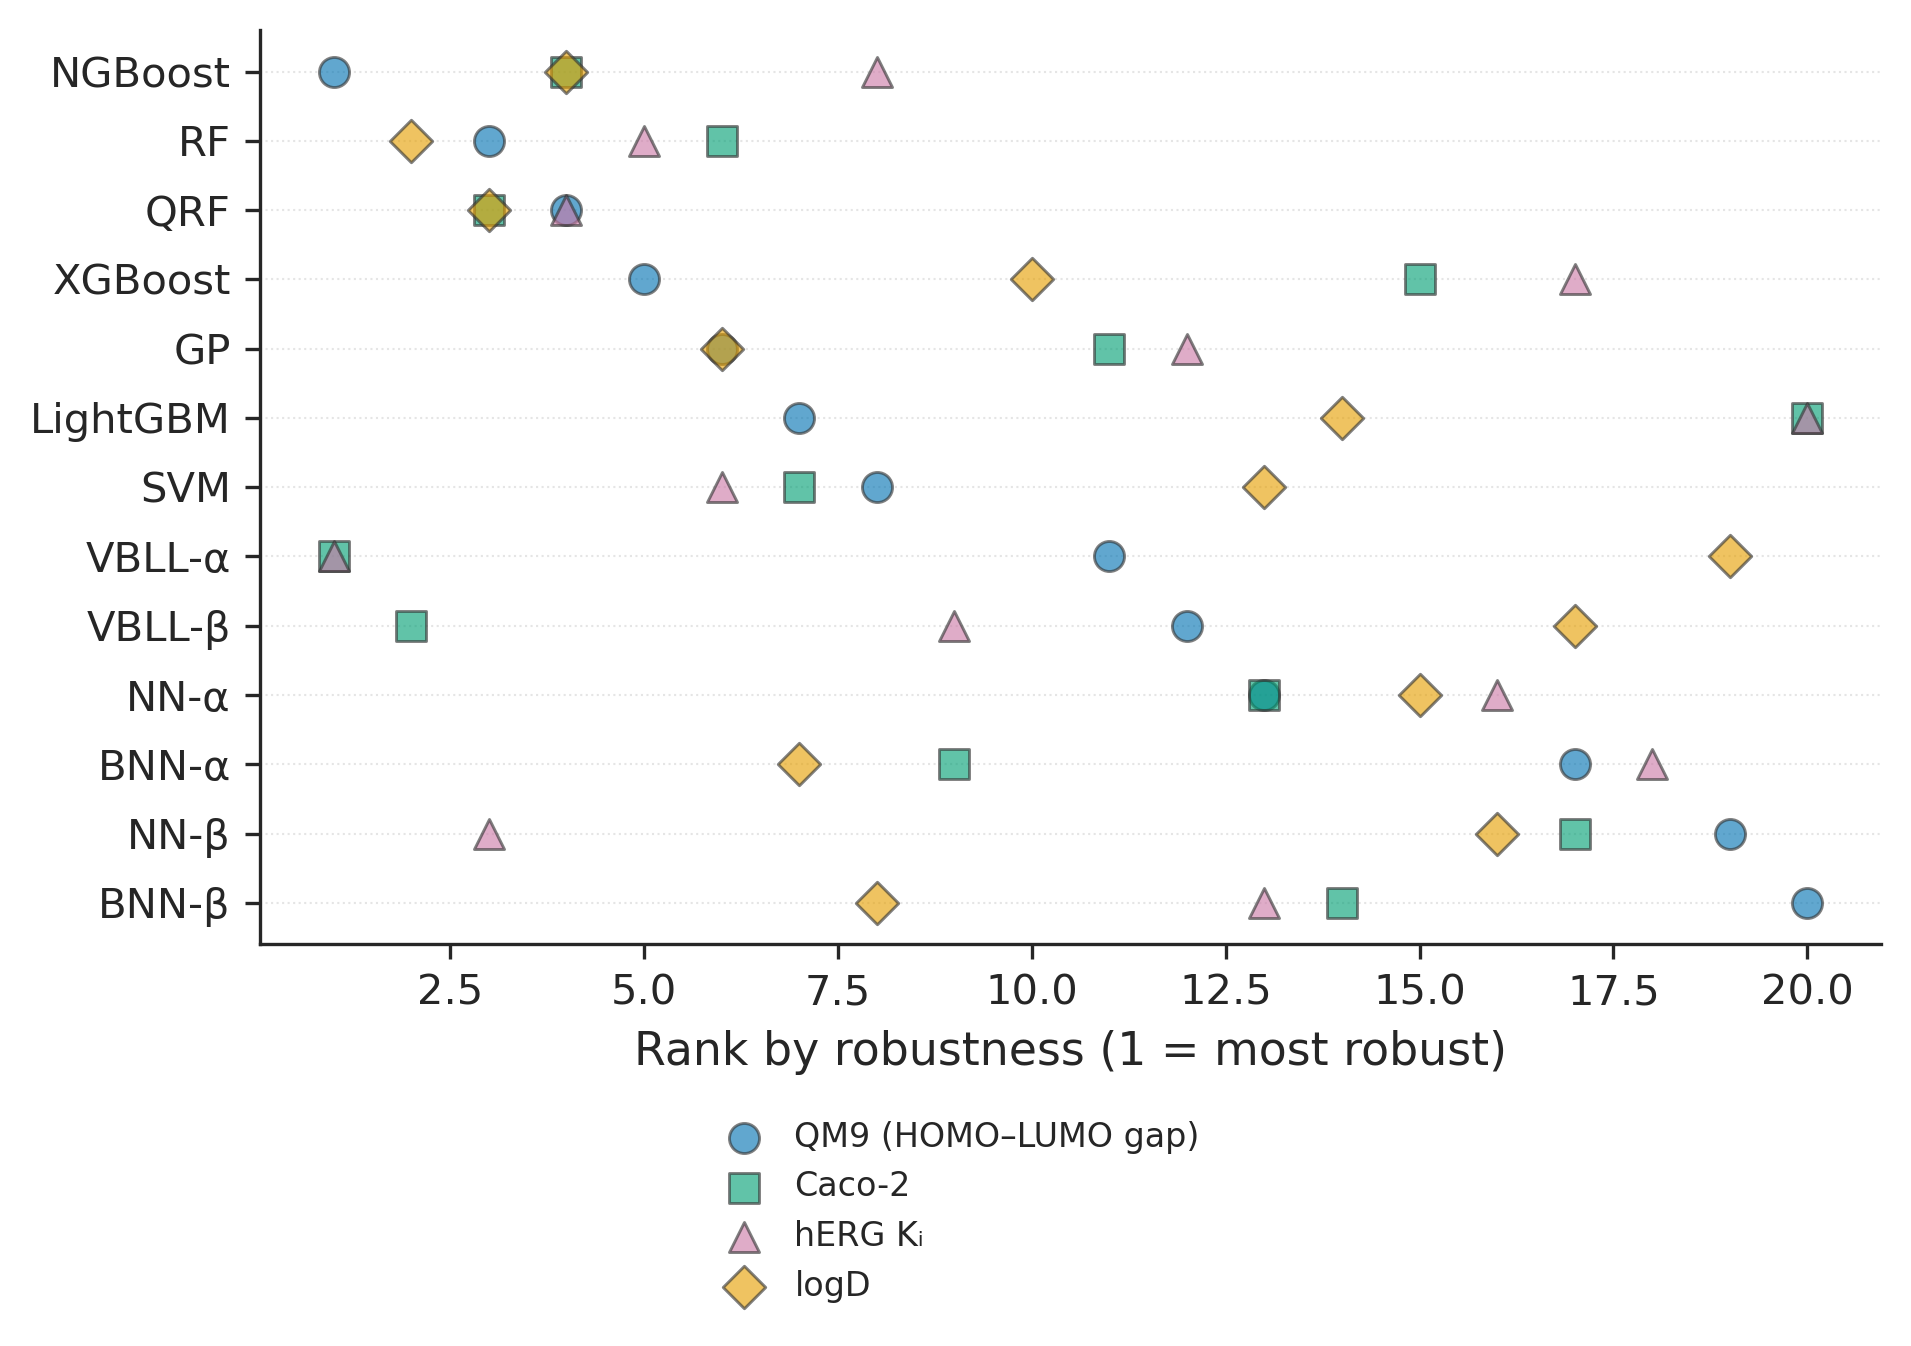
\includegraphics[width=\textwidth,height=0.72\textheight,keepaspectratio]{R9_rank_transfer_ecfp4.png}
\caption[Robustness rank of each model on QM9 and the three assay datasets.]{Rank by \aucnorm{} of each base model on every dataset, with ECFP4 under Gaussian noise.
Models are ordered by their rank on the QM9 HOMO--LUMO gap. Ranks are among all 19 models; the six variant models are not drawn.}
\label{fig:transfer}
\end{figure}

\section{Probabilistic and deterministic counterparts}

To further explore the impact of model architecture on noise robustness, we examined deterministic and probabilistic variants of the same core model architecture. The hypothesis was that a model that reports a distribution rather than a point value may be more robust to small amounts of injected label noise. We compared variants across three sets of base models: two NNs labeled NN-$\alpha$ and NN-$\beta$ and RF (Figure~\ref{fig:variants_change}). For each NN, we transform a standard deterministic network into a BNN. The BNNs with a variance head run at different settings from their Bayesian bases, so they are compared only for uncertainty. We compared RF to its probabilistic counterpart, QRF, with the same baseline architecture and hyperparameters. Comparisons of this nature are only possible when the variants carry the same underlying settings (Additional files~\ref{app:noise:sec:hyperparameters_default} and~\ref{app:noise:sec:hyperparameters_tuned}). NN-$\alpha$ and BNN-$\alpha$ therefore share one setting, as do NN-$\beta$ and BNN-$\beta$, and QRF is compared with a random forest of the same 300 trees (Additional file~\ref{app:noise:sec:hyperparameters_default}).

We compare RF and QRF directly with the same underlying architecture. QRF had lower \aucnorm{} on QM9 under Gaussian and grouped-shifted noise on every representation, and changed it little under grouped-wider noise, with almost no change in clean $R^2$ (Figure~\ref{fig:variants_change}). On the assay datasets QRF was less robust than RF under grouped-shifted noise on every dataset and representation, and under Gaussian noise on logD and hERG $K_i$ (Additional file~\ref{app:noise:sec:rf_vs_qrf_assay}). Under grouped-wider noise it was more robust on Caco-2 and mixed elsewhere.

The Bayesian transformations that we used to transform feed-forward deterministic NNs into probabilistic produced a slightly larger \aucnorm, but only because they lowered predictive performance on clean labels. BNN-$\beta$ kept more \aucnorm{} than NN-$\beta$ in most combinations on every assay dataset, and BNN-$\alpha$ on all assay datasets. On QM9 the Bayesian transformations made no significant change on either predictive performance or \aucnorm{} for either network.

\begin{figure}[!htbp]
\centering
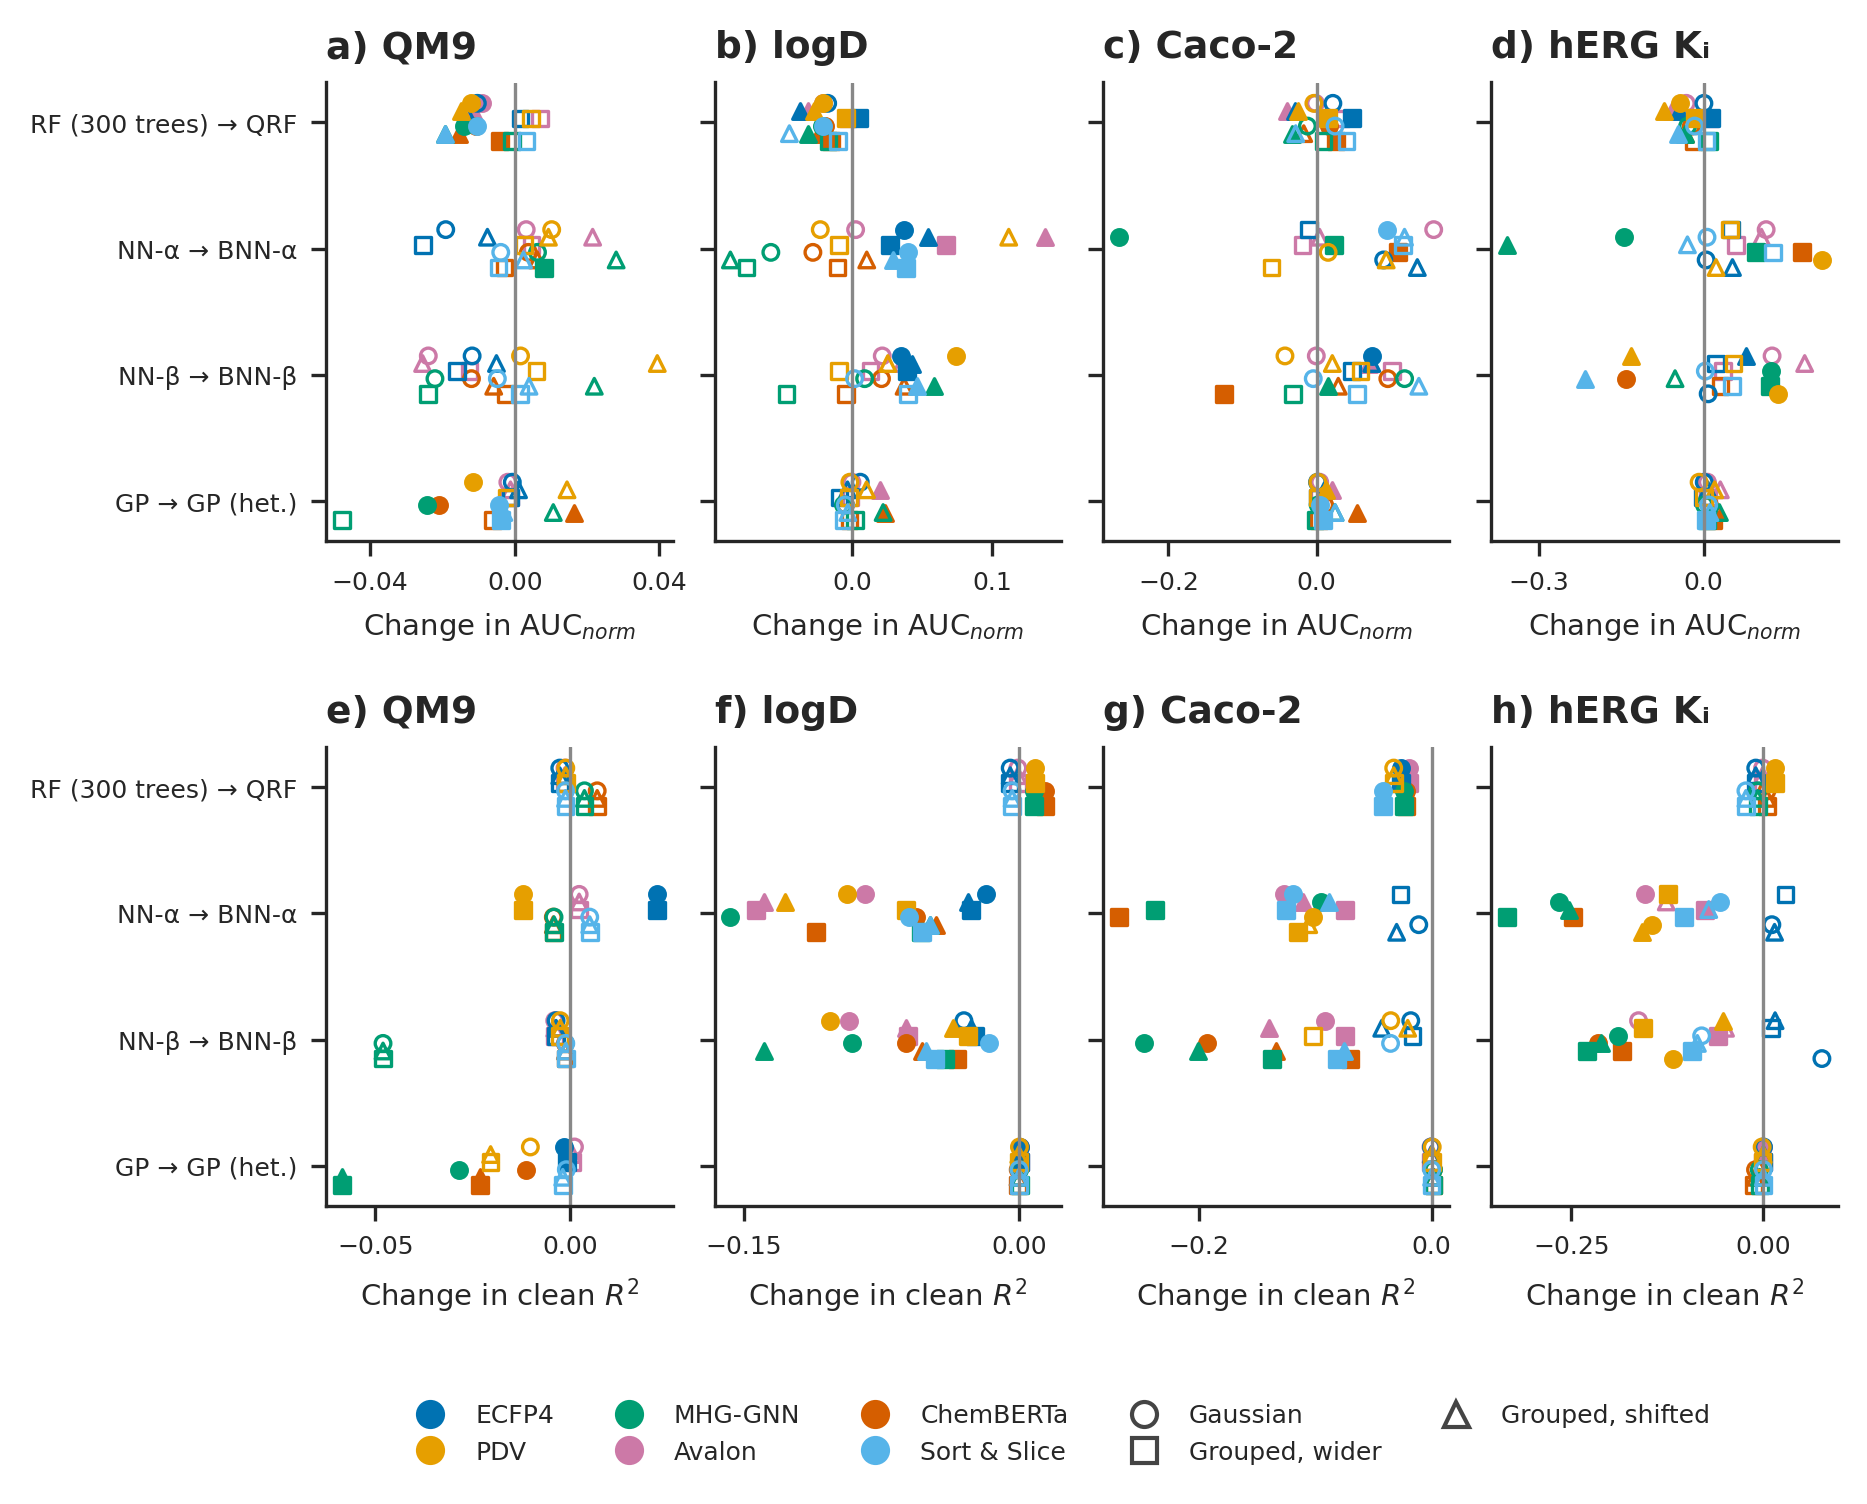
\includegraphics[width=\textwidth,height=0.72\textheight,keepaspectratio]{R17c_counterpart_changes.png}
\caption[Change from replacing a model with its probabilistic counterpart.]{Change in \aucnorm{} (top) and clean $R^2$ (bottom) from each model to its probabilistic
counterpart at the same settings, on every dataset: counterpart minus base, the median of paired differences over 10 replicates
on QM9 and five scaffold folds on the assay datasets. Color is the representation and shape the noise
condition. A filled mark changed in the same direction in every replicate or fold.}
\label{fig:variants_change}
\end{figure}

\section{Uncertainty under increasing label noise}\label{sec:uq}

Until now we've discussed how much predictive capabilities a model is able to retain while its training labels are corrupted with noise. Now, we consider how confident the model reports its own predictions are in the presence of noise, and whether or not those estimates match the increased label noise. \citet{Kolmar2021} found that the mean predicted uncertainty derived from the GPs increases with the amount of label noise in the training data. We go beyond the population level and instead ask if a model's per-sample uncertainty tracks label noise. One key sign that a model is able to handle noise is its ability to track it, represented by the per-sample Spearman correlation between predicted uncertainty and noise magnitude.

As expected, mean predicted uncertainty is positively correlated with Gaussian label noise for most models and representations (Table~\ref{tab:uncertainty_rise}). There are a few exceptions, namely BNN-$\beta$ on PDV and VBLL-$\beta$ (het.) on Avalon for QM9. BNN-$\alpha$ fails to rise in at least one fold on every assay dataset, and both full-BNNs with a variance head fail on MHG-GNN for hERG $K_i$, and BNN-$\beta$ with a variance head also fails on ChemBERTa and on Caco-2. \citet{Kolmar2021}'s finding therefore holds for almost every probabilistic model on the computed property, and for most of them on measured labels.

\begin{table}[!htbp]
\centering
\small
\begin{adjustbox}{max width=\textwidth,max totalheight=0.78\textheight}
\begin{tabular}{lcccccc}
\toprule
Model & QM9 & logD & Caco-2 & hERG $K_i$ & Aleatoric & Epistemic \\
\midrule
QRF & 4.9 & 2.7 & 2.4 & 2.3 & per molecule & per molecule \\
NGBoost & 4.8 & 3.2 & 2.6 & 2.6 & per molecule & none \\
GP & 5.3 & 4.1 & 2.5 & 2.6 & one per fit & per molecule \\
GP (het.) & --- & 4.3 & 2.7 & 2.8 & per molecule & per molecule \\
BNN-$\alpha$ & 3.4 & 1.4$\dagger$ & 1.0$\dagger$ & 1.4 & none & per molecule \\
BNN-$\alpha$ (var. head) & 4.1 & 2.7 & 1.9 & 2.1 & per molecule & per molecule \\
VBLL-$\alpha$ & 3.5 & 2.3 & 1.4 & 1.2 & one per fit & per molecule \\
VBLL-$\alpha$ (het.) & 3.0 & 1.9 & 2.8 & 3.5 & per molecule & per molecule \\
BNN-$\beta$ & 2.7$\dagger$ & 1.2$\dagger$ & 1.1 & 1.2 & none & per molecule \\
BNN-$\beta$ (var. head) & 4.3 & 2.5 & 2.4 & 1.7 & per molecule & per molecule \\
VBLL-$\beta$ & 3.3 & 2.4 & 1.3 & 1.2 & one per fit & per molecule \\
VBLL-$\beta$ (het.) & 2.6 & 2.0 & 2.7 & 3.1 & per molecule & per molecule \\
\bottomrule
\end{tabular}
\end{adjustbox}
\caption[Rise in mean predicted uncertainty under Gaussian noise.]{Mean predicted uncertainty on held-out molecules at a noise level of 1.5, divided by its value with no added noise, with PDV under Gaussian noise. $\dagger$: the uncertainty fails to rise in at least one fold. A dash: not run. Aleatoric and Epistemic: whether the model reports that component per molecule, as one value per fit, or not at all.}
\label{tab:uncertainty_rise}
\end{table}

\subsection{Aleatoric and epistemic attribution}

While this tells us that the models are reportedly less certain under noisy data, we don't know what the model is attributing this uncertainty to. To answer this question, we decompose uncertainty estimates into their aleatoric and epistemic components wherever possible. We expect to see aleatoric uncertainty rise with injected label noise, while the epistemic component should remain relatively constant, as it is the aleatoric component that describes uncertainty in the underlying data. The models whose frameworks allowed for this decomposition include full-BNNs with a variance head, the heteroscedastic GP, and QRF (Table~\ref{tab:uncertainty_rise}). The two heteroscedastic VBLL networks also report both components, and they separate them more often than any other model, though not on every dataset and representation. They are not drawn in the figures, as they were not scored out of fold.

The full-BNNs with a variance head behave as expected (Figure~\ref{fig:decomposition}), the epistemic component grows by at most 0.43 of the aleatoric growth in every configuration where the ratio can be computed. Despite QRF's strong predictive performance and noise robustness, both of its aleatoric and epistemic components rise with noise and on some representations, the epistemic component actually rises at a faster rate.

Unlike the predictive performance and robustness, the representation actually dictates whether decomposition works. For QRF, the epistemic growth is 0.61 to 1.14 times the aleatoric growth on the three fingerprints, 1.02 to 1.44 times on PDV, and 1.29 to 2.04 times on ChemBERTa and MHG-GNN. Under Gaussian noise the heteroscedastic GP keeps its epistemic growth below a quarter of its aleatoric growth on PDV, ChemBERTa and MHG-GNN except MHG-GNN on QM9, but not on ECFP4 under grouped-shifted noise, where the two grow by similar amounts.

The noise conditions follow the pattern found in robustness, the three conditions which alternate the noise distribution show similar decompositions to those under Gaussian noise, while group-shifted raises the epistemic share of the heteroscedastic GP and of QRF in every pairing of dataset and representation. This scaffold family-based offset may be appearing as structure in the data rather than label noise to the models.

\begin{figure}[!htbp]
\centering
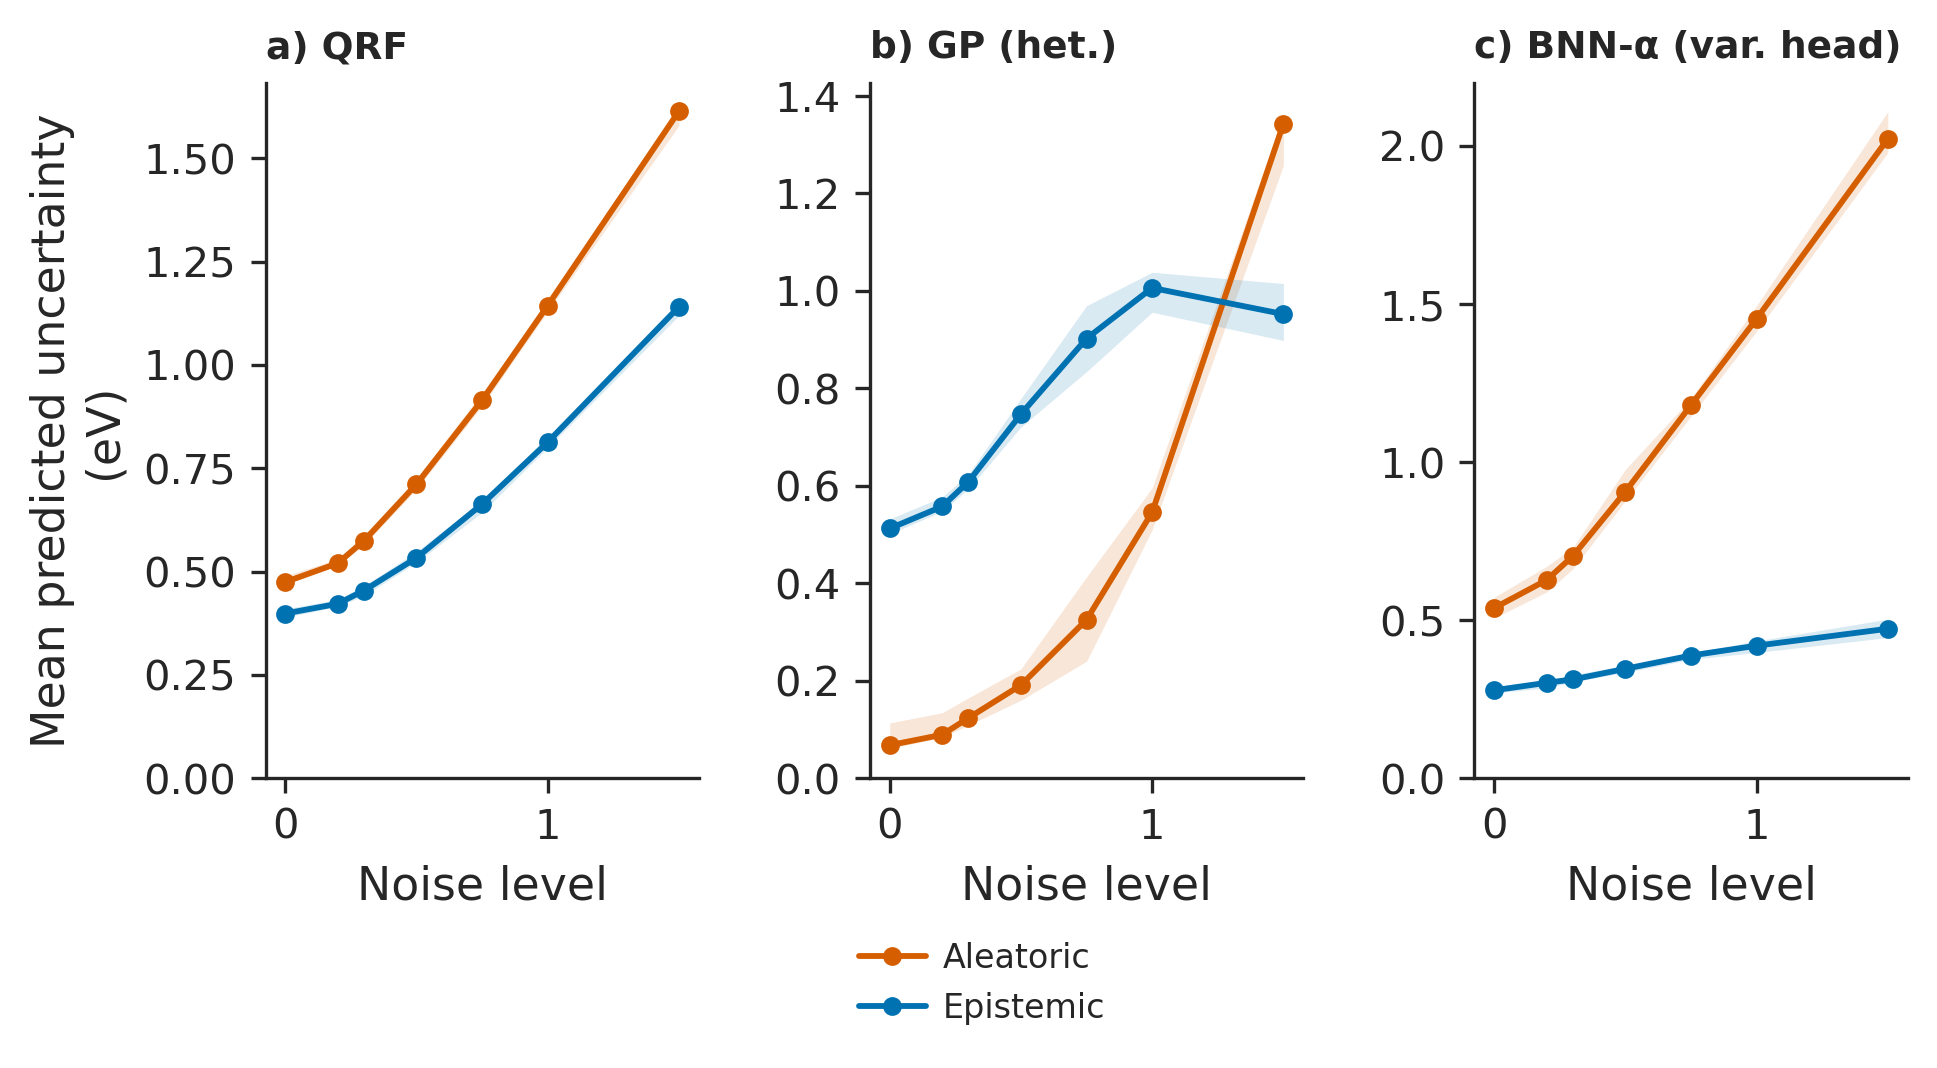
\includegraphics[width=\textwidth,height=0.72\textheight,keepaspectratio]{F6_decomposition.png}
\caption[Aleatoric and epistemic uncertainty against label noise on QM9.]{Aleatoric and epistemic components of the predicted uncertainty against noise level,
one panel per model, on the QM9 HOMO--LUMO gap with ECFP4 under Gaussian noise. Each value is the mean over the molecules
of one out-of-fold pass; lines are medians over folds and bands their range. A component that is one value
per fit is not drawn (Table~\ref{tab:uncertainty_rise}).}
\label{fig:decomposition}
\end{figure}

The aleatoric component indicates that label noise increased, but it doesn't tell us by how much (Figure~\ref{fig:aleatoric_injected}). For each unit of added noise it rises by roughly 0.4 to 1 unit, depending on model, dataset and representation. The aleatoric component can therefore compare noise between datasets or noise levels, but it does not estimate a dataset's internal error.

Uncertainty estimation breaks under censoring as the process of clipping the labels narrows their spread, which in turn shrinks the total uncertainty. None of the models tested treat a clipped label as a noisy one, so they actually grow more confident while losing information.

\begin{figure}[!htbp]
\centering
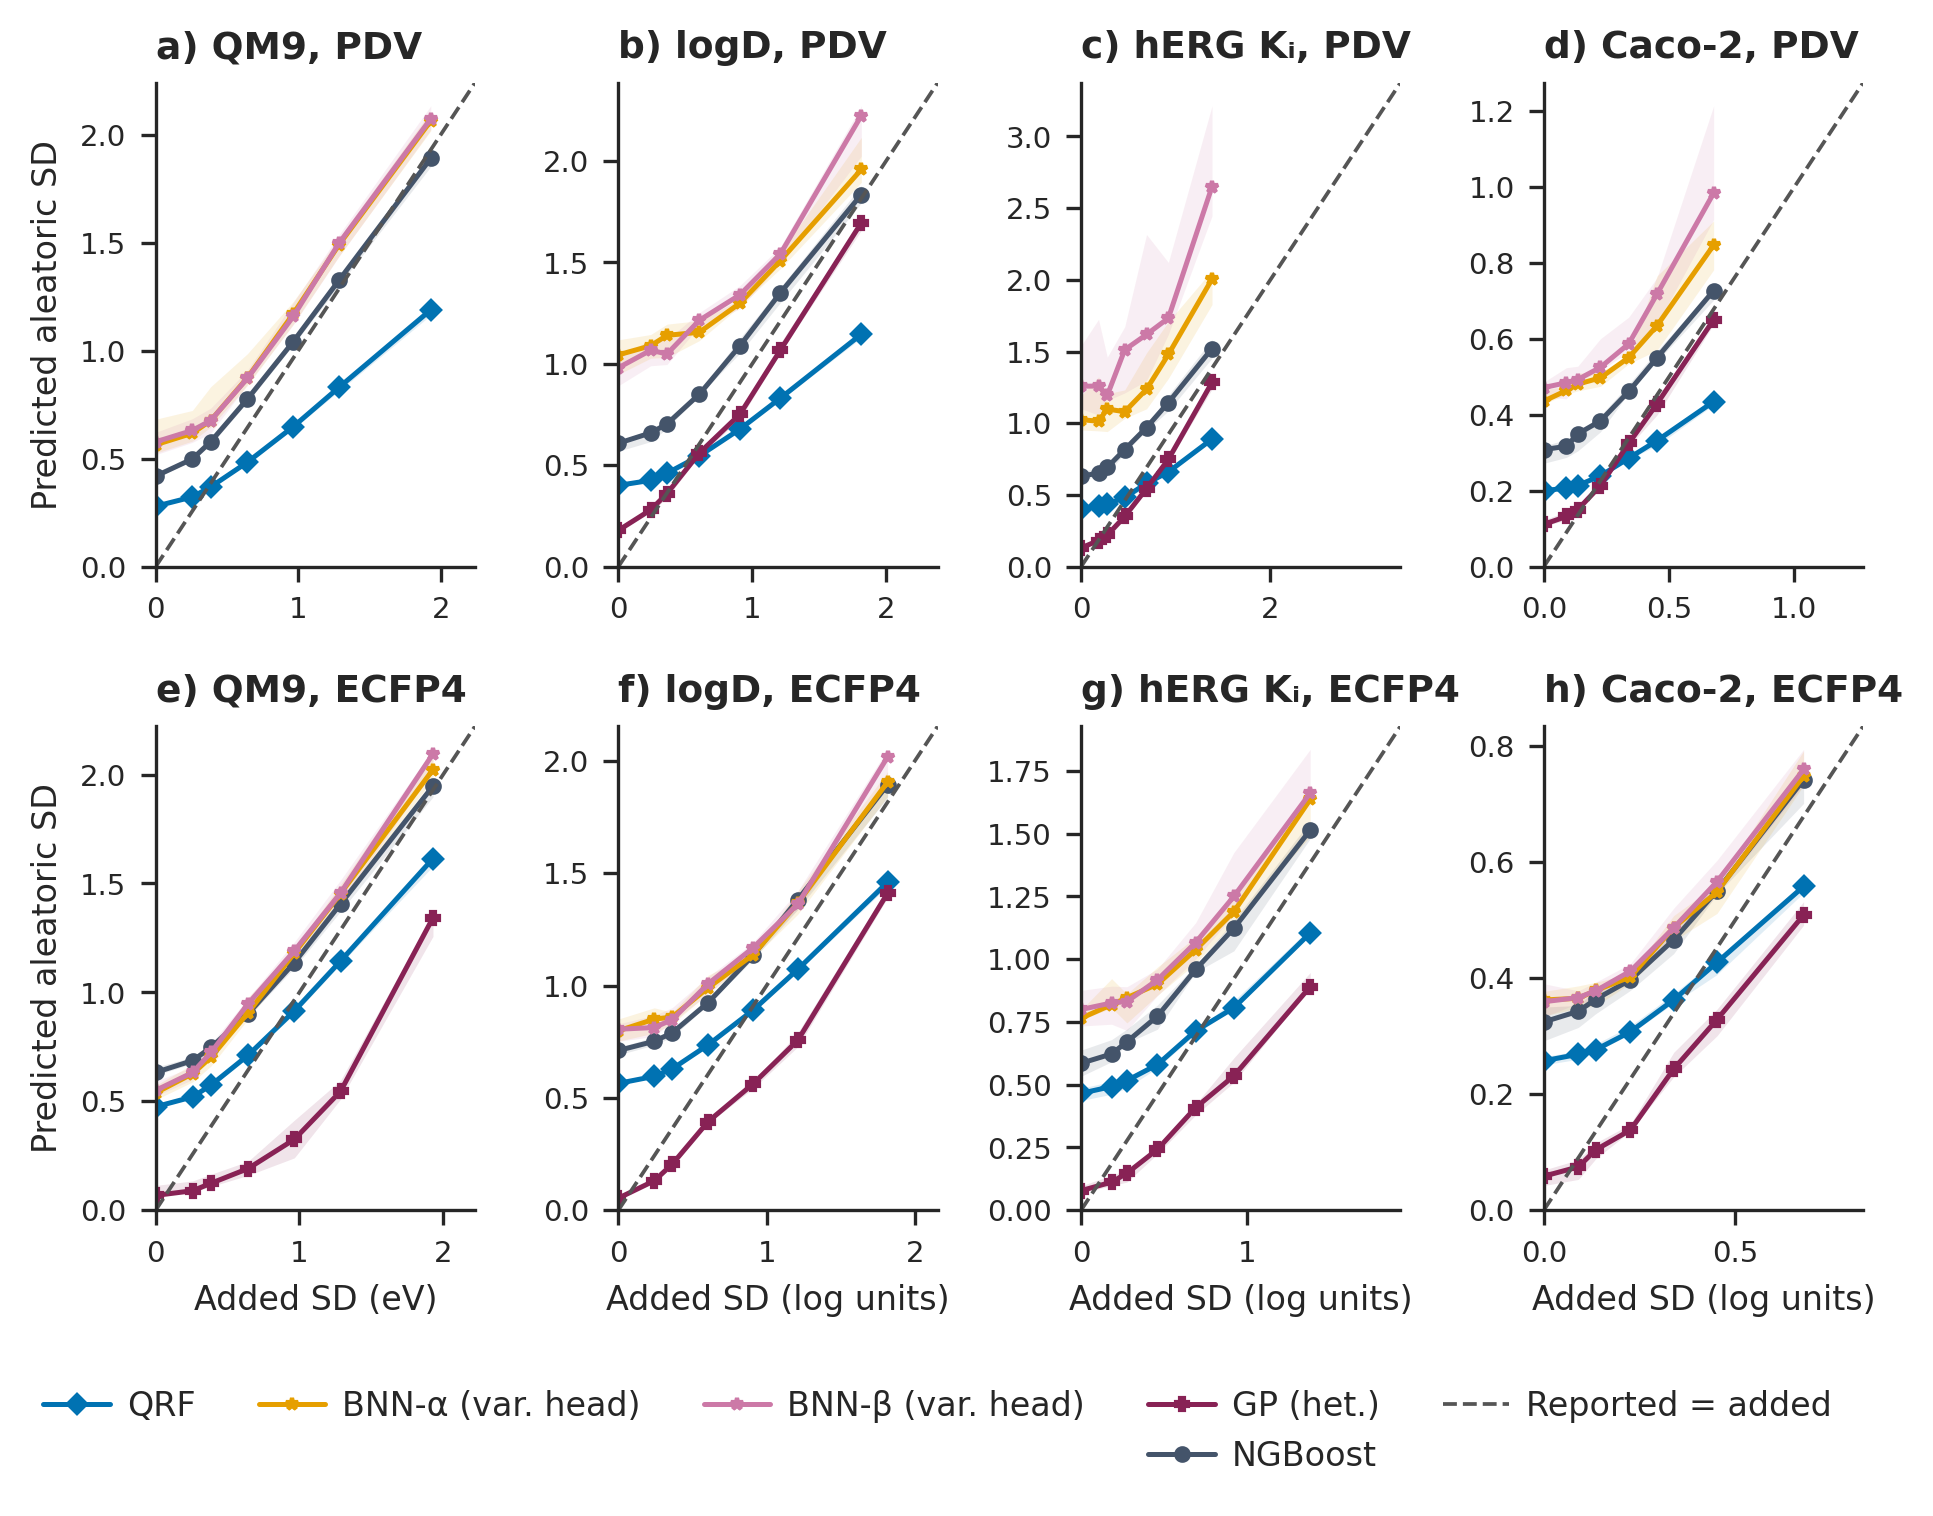
\includegraphics[width=\textwidth,height=0.72\textheight,keepaspectratio]{F6b_aleatoric_against_injected.png}
\caption[Aleatoric uncertainty against the added noise.]{Predicted aleatoric standard deviation against the standard deviation of the added noise,
under Gaussian noise. Rows are PDV (top) and ECFP4 (bottom); columns are the QM9 HOMO--LUMO gap, logD, hERG $K_i$
and Caco-2. Each line is one model: the median over folds of the mean over the molecules of one out-of-fold
pass, with a band spanning the folds. The dashed line is equality. The heteroscedastic Gaussian process was
not run on QM9 with PDV, and the two heteroscedastic variational networks were not scored out of fold.}
\label{fig:aleatoric_injected}
\end{figure}

\subsection{Per-sample uncertainty and label noise}\label{sec:uq_per_sample}

Finally, we ask whether a model's uncertainty on one molecule tracks the noise on that molecule's label. We assess this using the Spearman correlation between predicted uncertainty and the size of the injected noise over out-of-fold training molecules.

Since Gaussian, Laplace, Student-$t$ and grouped-shifted conditions add noise from the same scale to every label, there is not much for uncertainty to find. It's the same situation with outlier noise, under which a tenth of the data is chosen at random for extra noise, and with grouped-wider in which each scaffold family falls in a single fold, so a model makes predictions based on unseen scaffolds and has no basis for estimating uncertainty. The only case where per-sample uncertainty tracking is possible is censoring, as the noise is dependent on the value of the label itself. The correlations are then large and mostly negative, meaning the model is least uncertain on the labels that were clipped most. On QM9 with half the labels clipped, on PDV, they run from $-0.84$ to $-0.80$ across folds for NGBoost and from $-0.47$ to $-0.41$ for the GP, and on logD with half the labels clipped every fold of every model except the two GPs is at $-0.29$ or lower. We divided each molecule's error by its uncertainty and found that the division ranked the clipped labels better than the error alone on QM9 and on most of logD. Models are most confident on the clipped labels, probably because the clipping piles many labels into one value, which the model learns to tightly predict. Ironically, per-molecule uncertainty can be used in reverse to identify clipped labels as the labels a model is more certain about, especially when they fall in a certain range, are most likely to have been clipped.

\section{Conclusions}

We investigated how a variety of molecular representations and models perform under increasing label noise. We used ANOVA variance decomposition across three noise conditions on four datasets to show that molecular representation accounts for a larger share of the variance in predictive performance than in robustness. Robustness to label noise, as measured by \aucnorm, the normalized area under the $R^2$ retention curve, is more impacted by the choice of model. The representation each  model is paired with explains more variance than the representation alone. As such, a representation should not be chosen independently of the model it will be used with, and some models benefit from alternative molecular representations across both predictive performance and noise robustness. Model family was the primary factor in every decomposition except one,  Caco-2 under grouped-shifted noise, where the scaffold fold took the larger share.

Grouped-shifted and censored noise, the two conditions in which the error is systematic, corrupt QSAR model predictions the most. Changing the shape of the distribution from which noise is drawn barely has an impact on model performance, a conclusion which is in agreement with \citet{Heid2023}.
Low quantities of noise do not make much of an impact, on the HOMO--LUMO gap every base model keeps at least 93\% of its clean $R^2$ up to a noise level of 0.3, and grouped-shifted noise separates from the other conditions only from a level of 0.75 (Figure~\ref{fig:conditions}). Models' performance begins to degrade more rapidly on the assay datasets than on the HOMO--LUMO gap, which makes sense as assay data contain inherent experimental noise. Tree and kernel models maintained consistent \aucnorm{} across all representations, while the plain NNs and BNNs depended on the representation they were given, as did the predictive performance of NGBoost. Across datasets and noise conditions, RF and QRF were reliably robust, although their predictive performance on clean labels was middling and on Caco-2 they struggled under Gaussian noise. QRF was the slightly less robust of the two, falling below RF under Gaussian and grouped-shifted noise. Other models performed well only under some conditions. The GP had the highest predictive performance on clean labels and under independent noise but fell behind when the noise was shared within a scaffold family, NGBoost predicted well only with the right representation, and SVM led in predictive performance under scaffold-shared noise on some datasets. Transforming a feed-forward network into a Bayesian one increased \aucnorm, but the Bayesian variants never predicted better at any noise level, so switching to a tree-based model is the stronger move under label noise.

With regard to uncertainty estimation, mean predicted uncertainty rose with label noise for almost every probabilistic model on QM9 and for the majority of models on the assay datasets. Of the models whose aleatoric and epistemic components can be split per molecule, the BNNs with a variance head, the heteroscedastic GP and the heteroscedastic VBLL networks correctly attributed error from the injected noise as aleatoric, while QRF read that error as epistemic. The success of a split is also dependent on the representation, which is not necessarily the case for predictive performance or noise robustness. The aleatoric component rises by roughly 0.4 to 1 unit for each unit of noise added, so it can compare noise between datasets or between noise levels, but it does not measure a dataset's internal error. Outside censoring, no model's per-sample uncertainty identified which labels had been corrupted. Under censoring the models' most confident predictions are the clipped labels themselves, and dividing a molecule's error by its uncertainty picked out the clipped labels better than the error alone.

QM9 served as a relatively clean baseline as its properties are computed. The assay datasets containing experimental measurements on the endpoints LogD, Caco-2 \citep{openadmet}, and hERG $K_i$ \citep{Zdrazil2023} are smaller and cover a more narrow range of the chemical space. As the labels in these data are experimentally-derived and pooled from different laboratories, they contain some unknown amount of noise. We are then adding artificial noise on top of the existing experimental noise. These validation datasets supported the QM9 findings for the forests, with the boosted
trees XGBoost and LightGBM the notable exceptions, degrading on the external datasets. Future work should extend this type of noise robustness benchmarking to classification tasks and larger experimental datasets with better-known uncertainty estimates.

When training on noisy experimental data in the context of QSAR, it is important to keep in mind that a model's robustness to noise is primarily driven by its own mechanism of training, and to an extent the molecular representation the input data comes in, oftentimes with respect to the model. Of the models tested, RF was the most consistent choice across the four datasets, ranking between first and eighth for \aucnorm{} on every dataset, representation and noise condition. Where a predictive distribution is wanted, its probabilistic counterpart QRF maintains RF's predictive performance and nearly all of its noise robustness. What QRF cannot do is say where that uncertainty came from. Beyond the forests, the better choice depends on how much noise there is. LightGBM and XGBoost predict well on clean labels and lose the most as noise rises, so they suit data you trust, while NGBoost and the VBLL networks start lower and hold what they have.

In this research, we define a noise level as a fraction of the spread of the clean training labels. It is therefore relative to the dataset rather than an absolute measurement error, and cannot be mapped onto a given dataset exactly. There are other mechanisms used to estimate the noise in a dataset directly. When an assay's controls are available, the Z$'$-factor can be used to estimate noise \citep{Zhang1999}. You can also use screening data to test for row, column and plate effects, which produce systematic rather than independent error \citep{Caraus2015}. When you lack controls, replicates, and metadata, a label can be checked against the data itself. Confident learning flags labels by comparing each label to what a model predicts for that molecule when it was left out of training \citep{Northcutt2021}. You can use the point at which the model error matches the data's error to generate a predictive limit \citep{Kolmar2021, Crusius2024}. Beyond formal methods, you should consider how a dataset was assembled. How many independent replicates were done, how many laboratories contributed, whether assay protocols were consistently applied, and how varied are the compounds in chemical space?

The first limitation of this study is data availability. While HOMO--LUMO gap from QM9 is a good baseline as its computed labels carry no measurement error, it is only a single task. As the noise is meant to replicate experimental data, this analysis would be improved by more quality-controlled, relatively clean and well-replicated experimental data across different targets. However, data of that nature are hard to find publicly.

Second, \aucnorm{} is a ratio to clean $R^2$, so a model that starts from a low clean baseline has less to lose, and a few replicates scored above 1.05. We tried other measures of noise robustness, but they were either too strongly correlated with clean $R^2$ or did not capture the right quantity. The change in $R^2$ at a single noise level, for example, misses the shape of the curve. \aucnorm{} is not a perfect metric, but it describes the whole curve, and across the 13 base models it is unrelated to clean $R^2$.

Third, it is hard to draw conclusions that hold across so many conditions. No model or representation wins everywhere, although RF comes closest. When working with cheminformatics data, you don't know in advance how a model and representation will perform on the given prediction task. The underlying data is probably noisy, but you don't know how noisy it is or what shape that noise takes.

Given that, our recommendation is to test a handful of models against a handful of representations rather than tuning a single pairing, since on every dataset the pairing explains more of the variance in robustness than the representation does alone. The pattern of the noise should also guide that choice (Table~\ref{tab:condition_choice}). The same preferences held on all four datasets. Under Laplace, Student-$t$ and outlier noise, RF was the most robust model and SVM was the second. NGBoost lost \aucnorm{} under all three. Under grouped-wider noise, QRF was the most robust model and SVM was close behind. Of the boosted trees, XGBoost lost the most. Grouped-shifted noise was the hardest condition. Every model lost \aucnorm{} on every dataset and representation. RF lost the least of the models that also predicted well, and the GP lost the most. Gaussian noise was the only condition with a clear specialist. NGBoost was the most robust model on the HOMO--LUMO gap under Gaussian noise with every representation, but not on Caco-2 or hERG $K_i$.

% TODO: review -- table brought in from the repo-root copy of thesis.tex (~/repos/KIRBy/thesis.tex) and its rows rewritten to say what the paragraph above says. Removed from the old rows: SVM as the model to avoid under Gaussian noise, NGBoost "in the top two on five of six on logD", "NGBoost loses the most" under grouped-wider noise, and QRF "in the top three in every pairing". The Censoring row follows the censoring results earlier in this chapter, as the paragraph above does not mention censoring.
\begin{table}[!htbp]
\centering
\footnotesize
\begin{adjustbox}{max width=\textwidth,max totalheight=0.78\textheight}
\begin{tabular}{@{}p{0.13\linewidth}p{0.20\linewidth}p{0.20\linewidth}p{0.20\linewidth}p{0.20\linewidth}@{}}
\toprule
Noise condition & What it looks like & Prefer & Avoid & Extent of the evidence \\
\midrule
Gaussian
& Independent and symmetric, at the same scale on every label
& NGBoost, on the HOMO--LUMO gap
& ---
& NGBoost is the most robust model on the HOMO--LUMO gap with every representation, but not on Caco-2 or hERG $K_i$ \\
\addlinespace
Laplace, Student-$t$, outlier
& Independent but heavier-tailed, or concentrated on a random subset of labels
& RF first, SVM second
& NGBoost, which loses \aucnorm{} under all three
& All four datasets \\
\addlinespace
Grouped-wider
& Whole scaffold families receive a wider error than the other molecules
& QRF first, SVM close behind
& XGBoost, which loses the most of the boosted trees
& All four datasets \\
\addlinespace
Grouped-shifted
& Every scaffold family carries its own offset, so the error is systematic
& RF, which loses the least of the models that also predict well
& The GP, which loses the most; every model loses \aucnorm{} on every dataset and representation
& All four datasets; the hardest condition \\
\addlinespace
Censoring
& Labels above a limit are pulled down to that limit
& ---
& Every pair tested loses more robustness than under Gaussian noise
& The HOMO--LUMO gap only, on the five model and representation pairs run under censoring \\
\bottomrule
\end{tabular}
\end{adjustbox}
\caption[Which model to prefer under each noise condition.]{Which model to prefer under each noise condition. One row is one noise condition. A dash means no model is named.}
\label{tab:condition_choice}
\end{table}

These results follow from the loss function each model fits. NGBoost fits a per-molecule scale under a Gaussian likelihood, so it loses ground when the noise is not Gaussian. SVM ignores residuals that fall inside its margin, so it gains under the same conditions. QRF fits conditional quantiles, so a noisy scaffold family widens that family's interval without shifting the fit. Each boosting stage fits the residuals of the stage before it, and those residuals are largest in the noisy families. The GP is the most affected by error that is correlated with structure, because its kernel measures structure. None of this matters if the data are clean, as little separated the models below a noise level of 0.3.

In this chapter each model was given a standard molecular representation, and the choice of representation explained relatively little of the variance in noise robustness. We observe that this choice does impact the performance of different models to varying degrees, and the representations seem to capture different signals on each dataset that we tested. Chapter~\ref{chap:flaws} asks how well these representations compare molecules on a single dataset.

\chapter{Limitations of the Similarity Assumption}\label{chap:flaws}
% ---- TAKEAWAYS ----
% - General-purpose representations are built for all of chemistry. On one dataset, most of their features barely vary.
% - Some representations give different molecules exactly the same vector, mostly stereoisomers. No model can tell those molecules apart.
% - A similarity or distance compares every feature, so features irrelevant to the task dilute it. Different representations also disagree about which molecules are close.
% - Methods that judge a molecule by its neighbors did worst under label noise: LNL methods that use a distance, and noise detection by neighbors.
% - What is needed is a compact set of features chosen for the task from several representations. Chapter 5 builds it: the hybrid.
% ---- END TAKEAWAYS ----
% ---- NOTES: The Flaws of the Similarity Assumption ----
% Takeaway: before the first section, say that one section reuses the confirmation report's LNL study.
% Paragraph 1: a short preamble, opening with \textit{Preamble.} as in Chapter~\ref{chap:robustness}.
% - Section \ref{sec:lnl_motivation} reuses the exploratory learning-with-noisy-labels study from the DPhil confirmation report.
% - The report is titled "Investigating the Effects of Noise on Molecular Property Prediction". It is unpublished (January 2026).
% - The text and numbers of that section are identical or similar to the report. The rest of the chapter is new.
% - Cite it once here as \citet{Punt2026confirmation}.
% - refs.bib entry needed: @unpublished{Punt2026confirmation, author = {Punt, Adelaide}, title = {Investigating the Effects of Noise on Molecular Property Prediction}, note = {DPhil confirmation report, University of Oxford}, year = {2026}}.
% ---- END NOTES ----


\section{Introduction}

% [CLAUDE 2026-10-09] citation fix: Bajusz2015 does not say the choice matters little; Euclidean- and Manhattan-based similarities were not recommended.
The previous chapters have been focused on the impact of label noise. Before we delve into techniques that are meant to train on, identify, and mitigate such label noise, we first focus on a tangential point, molecular similarity. All of the aforementioned noise-adjacent methods, as well as the QSAR modeling itself, rest on the similar property principle (SPP; Section~\ref{sec:mol_similarity}), which posits that structurally similar compounds display similar chemical properties \citep{Johnson1990}. This serves as the conceptual foundation for QSAR modeling. The concept of molecular similarity is also used in various contexts to compare neighboring molecules. This comes into play when identifying noisy molecules that in theory stick out from their neighbors. There are some important exceptions to the SPP, namely activity cliffs \citep{Stumpfe2012, vanTilborg2022}. Furthermore, there is no single way to define similarity between compounds. This is where the principle begins to break down in practice. When defining similarity between two molecules, we typically rely on some pairwise mathematical function, or coefficient, that takes in two molecular representations as input. Two factors vary here, the representation and the coefficient. \citet{Bajusz2015} compared eight coefficients and found Tanimoto, Dice, Cosine and Soergel the best and largely equivalent, while similarities derived from Euclidean and Manhattan distances were not recommended on their own. In this chapter we ask if the standard methods of comparing molecules satisfy the SPP, insofar as they do not sufficiently quantify how similar two molecules actually are.

General-purpose molecular representations are designed to work across chemical domains. Consequently, when considering data from a specific domain, many of their features show little to no variance. Some representations assign separate molecules identical feature vectors. Since common fingerprints do not encode stereochemistry \citep{orsi2024map4c}, they are often unable to differentiate stereoisomers, which can have substantially different measured activity \citep{Nguyen2006}. As these coefficients compare every feature, irrelevant features dilute the result. Different representations also disagree about which molecules are close based on the information they carry. 

The problem of whether neighboring molecules can predict chemical activity has been measured before. The modelability index of \citet{Golbraikh2014} scores a binary dataset by the proportion of nearest-neighbor pairs that share an activity class, producing a single value for how strongly the similarity assumption holds on that particular combination of representation and data. It is not clear whether a low value is due to the data being intrinsically hard to model or to the representation not capturing adequate features for the task. Other work in this area relates to activity cliffs. \citet{Sheridan2020} compared experimental error, activity distribution and activity-cliff metrics as predictors of how well a dataset can be modeled, and found the cliff metrics the strongest of the three. However, they found that these metrics cannot separate real cliffs from those produced by uncertain activity measurements. \citet{MedinaFranco2013} point out that some of these activity cliffs are artifacts of the chosen representation, similarity threshold, or noise in the data. Activity cliffs are distinct from noise, as they carry some of the most valuable information about the interaction between structure and activity. None of these measures ask specifically about whether the specific features within these representations matter for the property at hand. 


% [CLAUDE 2026-10-09] citation fix: Riniker2013 used 88 targets from 3 collections; what correlated was screening performance; the 2 baselines are in addition to the 12.
We first consider how much the representation impacts similarity measures. \citet{Riniker2013} benchmarked 12 fingerprints and two simple baseline fingerprints for similarity-based virtual screening on 88 targets from three public collections, and found that the screening performance of the 12 fingerprints was highly correlated. Only the two baselines differed significantly from the rest. Neural embeddings were found to have a negligible improvement over ECFP across 25 pretrained models and 25 datasets \citep{Praski2025}. However, when looking into the differences between the structure of fingerprints, \citet{Huber2026} found that fingerprints which store raw counts are more effective at defining similarity than folded fingerprints when compared against a graph-based structural reference. Folding introduces bit collisions, which disproportionately distort similarity for molecules with many set bits \citep{Huber2026}. ACs follow the same pattern: across 15 configurations of representation and similarity measures on 3 datasets, the representations disagreed about which pairs form cliffs \citep{DabrowskiTumanski2026}, supporting the point \citet{MedinaFranco2013} make about ACs being artifacts of their representation. 

% [CLAUDE 2026-10-09] citation fix: Wilson1972 removes disagreeing samples; it does not smooth labels.
Any method that incorporates similarity measures, such as AC detection, or cleaning a training set by comparing each sample's label with its nearest neighbors' labels, whether by removing the samples that disagree \citep{Wilson1972} or by smoothing their labels, inherits this choice, as do the noise estimation and mitigation methods of this thesis. \citet{Coupry2022} learn a molecular similarity from graph embeddings, but independently of any endpoint. \citet{Zheng2000} did choose the similarity for the task. They predict each molecule's activity as the average over its $k$ most similar molecules by Euclidean distance over descriptors, and choose the descriptors by simulated annealing to maximize the leave-one-out $q^2$. \citet{Itskowitz2005} also optimize the number of neighbors and their weighting. Both select features for a nearest-neighbor model of one endpoint, whereas this thesis selects features across several representations.

The purpose of this chapter is to establish the problem that Chapter~\ref{chap:method} sets out to solve. Section~\ref{sec:flaws:representations} asks, for a given dataset, how much the features of standard representations vary and how many molecules map to identical feature vectors. Section~\ref{sec:flaws:similarity} asks what happens when these features are used to quantify similarity, and Section~\ref{sec:flaws:consequences} follows the consequences for methods built on these similarity measures, including an exploratory study of LNL methods (Section~\ref{sec:lnl_motivation}).


\section{Flaws in standard representations}\label{sec:flaws:representations}

General-purpose representations are built to span a broad range of chemical domains. When your dataset covers only a small region of the chemical space, a lot of the features within these generalized representations become irrelevant, describing chemistry which is absent from the data at hand. Pairwise comparisons of these representations rely on these irrelevant features.


\subsection{Constant and near-constant features}\label{sec:flaws:constant} 

To investigate similarity estimation, we first look at a simple measure: how many features vary within a dataset. A single dataset often contains a set of relatively similar molecules. Many features within a generalized representation contain information that describes all, or almost all, of the molecules in the set, failing to capture the variation between them. We define a constant feature to be one that takes a single value in every molecule of a dataset and a near-constant feature to be one that carries the same value in at least 95\% of the molecules. We counted constant and near-constant features from a set of representations (described in Table~\ref{tab:dataset_reps}) across hERG $K_i$, Caco-2, LogD, QM9, MDR1--MDCK efflux, human liver microsome (HLM) clearance, rat liver microsome (RLM) clearance and the Lhasa hERG blocker training set. HLM clearance and the Lhasa hERG set are not in Table~\ref{tab:dataset_reps}; their base representations are those with counts in Table~\ref{tab:constant_features_b}.

The substructure-based fingerprints have the most near-constant features. The learned embeddings, which are taken from the last layers of a NN, have none except MHG-GNN (Tables~\ref{tab:constant_features} and~\ref{tab:constant_features_b}, Figure~\ref{fig:constant_features}). ECFP4 is the worst offender. On hERG $K_i$ (1,412 molecules) 1,815 of the 2,048 features are near-constant. That jumps to 1,997 out of 2,048 near-constant features for the HOMO--LUMO gap on QM9. 292 of MHG-GNN's 1,024 features are zero in every molecule across all seven datasets that used it. They come directly from the saved encoder output rather than the data, and we have not looked into why. 

\begin{figure}[!htbp]
\centering
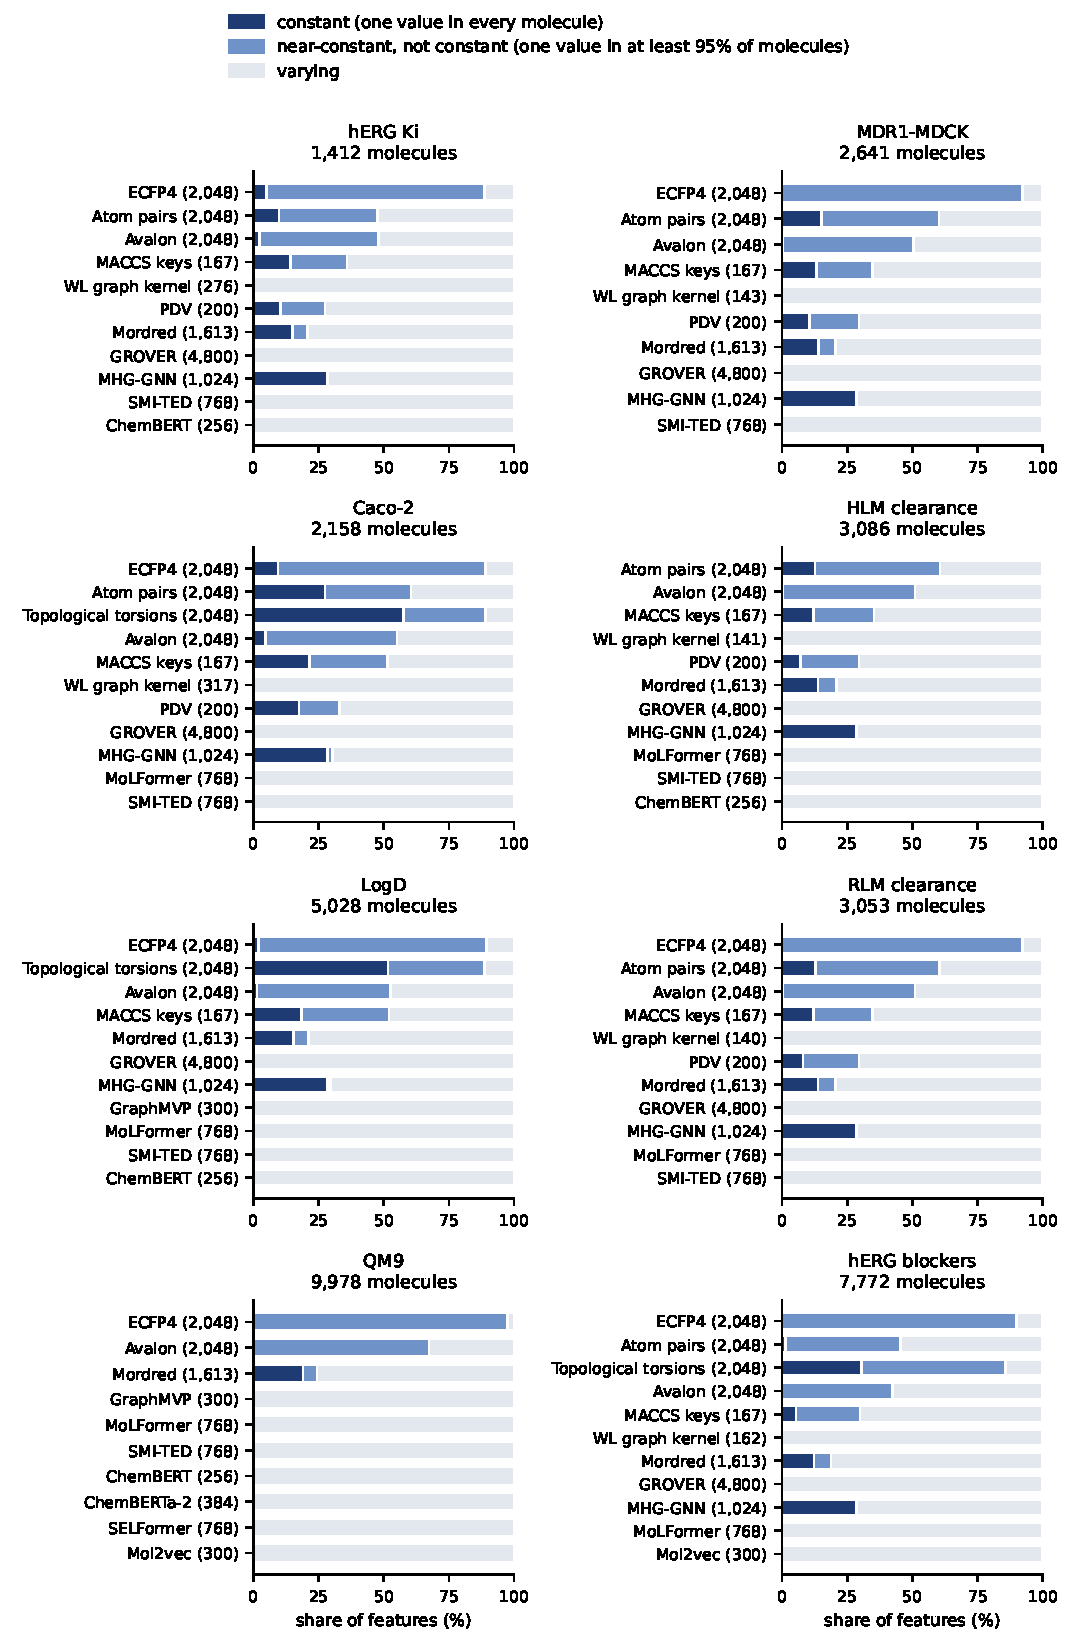
\includegraphics[width=\textwidth,height=0.72\textheight,keepaspectratio]{figures_code_input/constant_features.pdf}
\caption[Shares of constant, near-constant and varying features per representation.]{Shares of constant (dark blue), near-constant (mid blue) and varying (gray) features of each representation on eight datasets. The number of features of each representation is in parentheses.}
\label{fig:constant_features}
\end{figure}

These constant counts are sometimes filtered out by the distance. Tanimoto similarity (Equation~\ref{eq:tanimoto}; the distance is $1-T$) ignores bits off in both molecules, but a bit on in every molecule raises every molecule's measured similarity. It does not use the 105 constant ECFP4 bits on hERG $K_i$. Constant features add zero to a Euclidean or Manhattan distance; however, near-constant features are amplified. That's great behavior if those features define an AC. If not, they are contributing disproportionately to the measure of similarity. 


\begin{table}[htbp]
\centering
\small
\setlength{\tabcolsep}{4pt}
\begin{adjustbox}{max width=\textwidth,max totalheight=0.78\textheight}
\begin{tabular}{lrcccc}
\toprule
Representation & Features & hERG $K_i$ & Caco-2 & LogD & QM9 \\
 & & (1,412) & (2,158) & (5,028) & (9,978) \\
\midrule
ECFP4 & 2,048 & 105 / 1,815 & 194 / 1,826 & 39 / 1,834 & 0 / 1,997 \\
Atom pairs & 2,048 & 201 / 977 & 563 / 1,239 & -- & -- \\
Topological torsions & 2,048 & -- & 1,179 / 1,822 & 1,059 / 1,818 & -- \\
Avalon & 2,048 & 50 / 985 & 98 / 1,128 & 30 / 1,076 & 4 / 1,380 \\
MACCS keys & 167 & 24 / 60 & 36 / 86 & 31 / 87 & n/a \\
WL graph kernel & 140--317 & 0 / 0 / 276 & 0 / 0 / 317 & -- & -- \\
PDV & 200 & 21 / 55 & 35 / 66 & -- & -- \\
Mordred & 1,613 & 242 / 336 & -- & 247 / 340 & 307 / 394 \\
GROVER & 4,800 & 0 / 0 & 0 / 0 & 0 / 0 & -- \\
MHG-GNN & 1,024 & 292 / 292 & 292 / 310 & 292 / 304 & -- \\
GraphMVP & 300 & -- & -- & 0 / 0 & 0 / 0 \\
MoLFormer & 768 & -- & 0 / 0 & 0 / 0 & 0 / 0 \\
SMI-TED & 768 & 0 / 0 & 0 / 0 & 0 / 0 & 0 / 0 \\
ChemBERT & 256 & 0 / 0 & -- & 0 / 0 & 0 / 0 \\
ChemBERTa-2 & 384 & -- & -- & -- & 0 / 0 \\
SELFormer & 768 & -- & -- & -- & 0 / 0 \\
Mol2vec & 300 & -- & -- & -- & 0 / 0 \\
\bottomrule
\end{tabular}
\end{adjustbox}
\caption[Constant and near-constant features per representation, part 1.]{Constant and near-constant features of each representation on hERG $K_i$, Caco-2, LogD and QM9, with the number of molecules under each dataset name. Each entry gives the number of constant features and the number of near-constant features (one value in at least 95\% of molecules); WL graph kernel entries add its number of features, which varies by dataset. A dash marks a representation outside the dataset's base representations, and n/a one that was not computed.}
\label{tab:constant_features}
\end{table}

\begin{table}[htbp]
\centering
\small
\setlength{\tabcolsep}{4pt}
\begin{adjustbox}{max width=\textwidth,max totalheight=0.78\textheight}
\begin{tabular}{lrcccc}
\toprule
Representation & Features & MDR1--MDCK & HLM clearance & RLM clearance & hERG blockers \\
 & & (2,641) & (3,086) & (3,053) & (7,772) \\
\midrule
ECFP4 & 2,048 & 1 / 1,890 & -- & 1 / 1,887 & 0 / 1,840 \\
Atom pairs & 2,048 & 308 / 1,233 & 260 / 1,240 & 262 / 1,238 & 28 / 929 \\
Topological torsions & 2,048 & -- & -- & -- & 625 / 1,754 \\
Avalon & 2,048 & 5 / 1,032 & 8 / 1,044 & 8 / 1,045 & 0 / 866 \\
MACCS keys & 167 & 22 / 58 & 20 / 59 & 20 / 58 & 9 / 50 \\
WL graph kernel & 140--317 & 0 / 0 / 143 & 0 / 0 / 141 & 0 / 0 / 140 & 0 / 0 / 162 \\
PDV & 200 & 21 / 59 & 14 / 59 & 16 / 59 & -- \\
Mordred & 1,613 & 226 / 331 & 222 / 336 & 222 / 331 & 197 / 304 \\
GROVER & 4,800 & 0 / 0 & 0 / 0 & 0 / 0 & 0 / 0 \\
MHG-GNN & 1,024 & 292 / 292 & 292 / 293 & 292 / 293 & 292 / 292 \\
MoLFormer & 768 & -- & 0 / 0 & 0 / 0 & 0 / 0 \\
SMI-TED & 768 & 0 / 0 & 0 / 0 & 0 / 0 & -- \\
ChemBERT & 256 & -- & 0 / 0 & -- & -- \\
Mol2vec & 300 & -- & -- & -- & 0 / 0 \\
\bottomrule
\end{tabular}
\end{adjustbox}
\caption[Constant and near-constant features per representation, part 2.]{Constant and near-constant features of each representation on MDR1--MDCK efflux, HLM clearance, RLM clearance and the Lhasa hERG blocker training set of 7,772 molecules. Entries read as in Table~\ref{tab:constant_features}.}
\label{tab:constant_features_b}
\end{table}

\subsection{Molecules with identical feature vectors}

A standard fingerprint- or descriptor-based representation can produce the same feature vector for two separate molecules. In turn, models using this representation will produce a single prediction for the molecules with identical features. Identical feature vectors do not always mean that the representation has merged two different molecules, since a dataset pooled from several sources can hold two measurements of the same molecule.

Many fingerprints are computed without stereochemistry \citep{orsi2024map4c}. In this research, ECFP4 is built with stereochemistry off, and the 2D descriptor sets (PDV, Mordred) also ignore it, so almost every molecule they produce identical representations for is a stereoisomer of another (Table~\ref{tab:flaws:ties}). Any representation that reads from these subsequently merges stereoisomers. Additionally, methods using the Weisfeiler--Lehman relabeling scheme are bounded by the 1-Weisfeiler--Lehman test (Chapter~\ref{chap:background}), so some non-isomorphic graphs also receive the same vector. This is seen in the graph-kernel features which tie 105 of 1,412 hERG $K_i$ molecules, 56 of which differ only in stereochemistry and 49 in more than that. 

Whether or not a learned embedding is able to differentiate stereoisomers is dependent on its input as well as its individual implementation. SMI-TED, a pretrained SMILES encoder, ties 56 hERG $K_i$, 633 LogD and 177 Caco-2 molecules, all stereoisomers. A tokenizer can drop stereochemistry prior to training. The tokenizer of the ChemBERTa-77M-MTR checkpoint (ChemBERTa-2 in Table~\ref{tab:constant_features}, called ChemBERTa in Chapter~\ref{chap:robustness}) gives 72 of the 1,415 hERG $K_i$ molecules of Chapter~\ref{chap:robustness} the same token sequence as another molecule. Since stereoisomers can differ in measured activity \citep{Nguyen2006}, these representations lack potentially useful chemical information. 

% TODO: review, needs manual review -- simplified rewrite of the block you flagged as "completely lost"; no numbers changed, the mean group spreads (0.28 and 0.39 pKi) were dropped
% ==== CODE INPUT: new, needs review ====
We counted these ties on hERG $K_i$, LogD and Caco-2, for each dataset's base representations and augmentation features (small feature sets added to the hybrid after it is built, Chapter~\ref{chap:method}, ``Augmentation''). Two molecules are tied when a representation gives them exactly the same feature vector. No tie came from one compound listed twice (checked by InChIKey) or from a row of zeros, so every tie merges two different molecules (Table~\ref{tab:flaws:ties}).

Apart from the MACCS keys, most tied molecules are stereoisomers. Atom pairs, PDV, Mordred and SMI-TED tie only stereoisomers, and ECFP4, Avalon and topological torsions add a few molecules that differ in more than their stereochemistry. On hERG $K_i$, ECFP4, atom pairs, PDV, Mordred and SMI-TED tie the same 56 molecules, so joining any of these five representations leaves all 56 tied. The WL graph kernel also ties 49 hERG $K_i$ and 26 Caco-2 molecules that are not stereoisomers, and the MACCS keys tie the most molecules on every dataset, mostly not stereoisomers. The 3D augmentation features and the learned embeddings ChemBERT, GROVER, MHG-GNN, MoLFormer and GraphMVP tie none, and joining all of a dataset's representations leaves no molecule tied. % CHECK: the ChemBERT count comes from the cached chembert.npy (256 features). Whether that cache matches the current featurizer code is unverified.

A model has to give every molecule in a tied group the same prediction. The best single prediction for a group is its mean label, so ties set an error that no model can go below,
\begin{equation}
\mathrm{RMSE}_{\min} = \sqrt{\frac{1}{n}\sum_{G}\sum_{i \in G}\left(y_i - \bar{y}_G\right)^2},
\end{equation}
where $n$ is the number of molecules, $G$ runs over the tied groups and $\bar{y}_G$ is the mean label of group $G$. The matching best $R^2$ is $1 - \mathrm{RMSE}_{\min}^2 / \mathrm{Var}(y)$. On hERG $K_i$ this lowest error is at most $0.134$ p$K_i$ (MACCS keys), small next to the label standard deviation of $0.915$ p$K_i$.

% [CLAUDE 2026-10-09] citation fix: Kramer2012 reports mean error 0.44, SD 0.54, median 0.34 pKi; 0.54 is the SD, not the typical difference.
Single groups can still disagree by a lot. Independent p$K_i$ measurements of the same compound against the same target differ by $0.44$ log units on average, with a standard deviation of $0.54$ \citep{Kramer2012}, so a gap larger than $0.54$ inside a tied group is larger than typical measurement noise. On hERG $K_i$, 6 of the 26 ECFP4 groups and 38 of the 153 MACCS groups differ by more than $0.54$. The widest ECFP4 group is a pair of stereoisomers $1.14$ p$K_i$ apart (Figure~\ref{fig:flaws:stereo_pair}). An ECFP4 model can at best predict their mean, $5.59$ p$K_i$, which leaves each molecule $0.57$ p$K_i$ from its measured value.

\begin{figure}[!htbp]
\centering
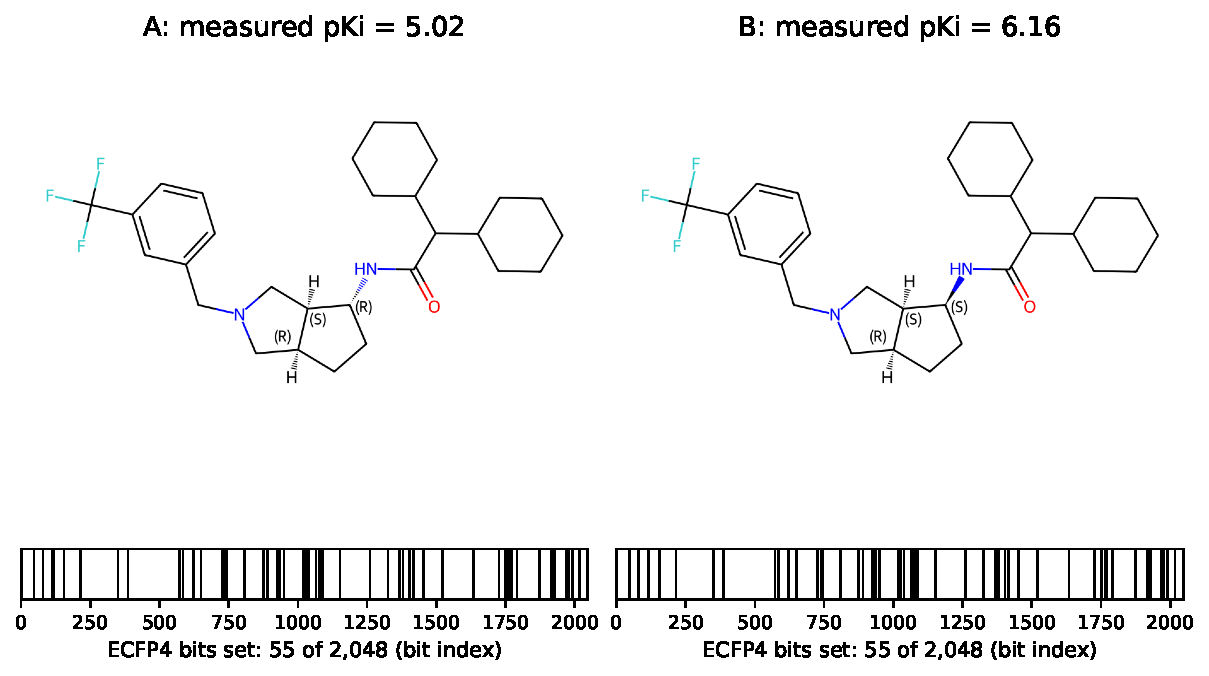
\includegraphics[width=\textwidth,height=0.72\textheight,keepaspectratio]{figures_code_input/herg_ki_ecfp4_stereo_pair.pdf}
\caption[Two hERG $K_i$ stereoisomers with identical ECFP4 vectors.]{Two hERG $K_i$ stereoisomers with identical ECFP4 vectors, which differ at the carbon bearing the amide nitrogen (R in A, S in B). The top row shows the structures with their measured p$K_i$ values, and the bottom row shows the 55 of 2,048 ECFP4 bits set in both.}
\label{fig:flaws:stereo_pair}
\end{figure}

A tied pair with different labels is also the most extreme activity cliff possible. The structure--activity landscape index of molecules $i$ and $j$,
\begin{equation}
\mathrm{SALI}_{ij} = \frac{|y_i - y_j|}{1 - \mathrm{sim}(i,j)}
\end{equation}
\citep{Guha2008}, is infinite when their similarity is 1 and their labels differ, and here the cliff is made by the representation rather than the chemistry. A method that judges a label by its nearest neighbors sees a tied neighbor at distance 0 with a different label, and may flag a correct label as noise (Section~\ref{sec:flaws:neighbors}).

% Table: one row per dataset x representation that ties any molecule.
\begin{table}[htbp]
\centering
\small
\setlength{\tabcolsep}{4pt}
\begin{adjustbox}{max width=\textwidth,max totalheight=0.78\textheight}
\begin{tabular}{llrrrrrr}
\toprule
Dataset & Representation & Molecules & Tied & Stereo- & Best & Best & Largest \\
 & & & & only & RMSE & $R^2$ & spread \\
\midrule
hERG $K_i$ (p$K_i$) & ECFP4 & 1,412 & 56 (4.0\%) & 56 & 0.041 & 0.998 & 1.14 \\
 & Atom pairs & 1,412 & 56 (4.0\%) & 56 & 0.041 & 0.998 & 1.14 \\
 & PDV & 1,412 & 56 (4.0\%) & 56 & 0.041 & 0.998 & 1.14 \\
 & Mordred & 1,412 & 56 (4.0\%) & 56 & 0.041 & 0.998 & 1.14 \\
 & SMI-TED & 1,412 & 56 (4.0\%) & 56 & 0.041 & 0.998 & 1.14 \\
 & Avalon & 1,412 & 66 (4.7\%) & 56 & 0.049 & 0.997 & 1.20 \\
 & WL graph kernel & 1,412 & 105 (7.4\%) & 56 & 0.071 & 0.994 & 1.49 \\
 & MACCS keys (aug.) & 1,412 & 377 (26.7\%) & 30 & 0.134 & 0.978 & 1.80 \\
\midrule
LogD (log units) & ECFP4 & 5,028 & 641 (12.7\%) & 633 & 0.044 & 0.999 & 1.00 \\
 & Mordred & 5,028 & 633 (12.6\%) & 633 & 0.043 & 0.999 & 1.00 \\
 & SMI-TED & 5,028 & 633 (12.6\%) & 633 & 0.043 & 0.999 & 1.00 \\
 & Avalon & 5,028 & 647 (12.9\%) & 629 & 0.047 & 0.998 & 1.40 \\
 & Topological torsions & 5,028 & 675 (13.4\%) & 631 & 0.047 & 0.998 & 1.10 \\
 & MACCS keys (aug.) & 5,028 & 2,343 (46.6\%) & 437 & 0.220 & 0.965 & 2.80 \\
\midrule
Caco-2 (log units) & ECFP4 & 2,158 & 179 (8.3\%) & 177 & 0.027 & 0.996 & 0.74 \\
 & Atom pairs & 2,158 & 177 (8.2\%) & 177 & 0.027 & 0.996 & 0.74 \\
 & PDV & 2,158 & 177 (8.2\%) & 177 & 0.027 & 0.996 & 0.74 \\
 & SMI-TED & 2,158 & 177 (8.2\%) & 177 & 0.027 & 0.996 & 0.74 \\
 & Avalon & 2,158 & 181 (8.4\%) & 177 & 0.027 & 0.996 & 0.74 \\
 & Topological torsions & 2,158 & 186 (8.6\%) & 177 & 0.029 & 0.996 & 0.74 \\
 & WL graph kernel & 2,158 & 203 (9.4\%) & 177 & 0.028 & 0.996 & 0.74 \\
 & MACCS keys (aug.) & 2,158 & 804 (37.3\%) & 139 & 0.111 & 0.935 & 1.72 \\
\bottomrule
\end{tabular}
\end{adjustbox}
\caption[Molecules that share a feature vector with another molecule.]{Molecules that share their feature vector with at least one other molecule, one row per representation that ties any molecules. Tied gives the number and share of such molecules, and Stereo-only those tied only with their own stereoisomers. Best RMSE and best $R^2$ are the best any model can reach given the ties. Best RMSE and Largest spread, the largest label range within one tied group, are in the units beside the dataset name, and (aug.) marks an augmentation representation.}
\label{tab:flaws:ties}
\end{table}

% ==== END CODE INPUT ====


\section{Flaws in similarity and other pairwise computations}\label{sec:flaws:similarity} 

Section~\ref{sec:flaws:representations} described some of the limitations of standard representations. Here we ask what happens when two molecules are compared through one of them, as these pairwise comparisons (Chapter~\ref{chap:background}) can violate the SPP.


% [CLAUDE 2026-10-09] citation fix: LopezPerez2024 calls Tanimoto the most popular metric, not Tanimoto-on-ECFP the standard; the 'coefficient of choice' quote is Willett 2006, quoted in Bajusz2015.
% [CLAUDE 2026-10-09] citation fix: Capecchi2020 removed chirality before the analysis; the ties are not stereoisomers.
The Tanimoto coefficient is the most popular similarity metric in cheminformatics \citep{LopezPerez2024}, and is commonly computed on ECFPs, although the coefficient applies to any bit vector. It has been described as the ``coefficient of choice'' for molecular similarity \citep{Willett2006}, while the Morgan fingerprint, ECFP4 in this research, ranks among the strongest fingerprints for virtual screening and target prediction \citep{Capecchi2020}. ECFP4 and ECFP6 specifically, alongside topological torsion, rank among the best of 28 fingerprints tested for ordering diverse structures by similarity \citep{OBoyle2016}. However, it is not a one-size-fits-all solution. Across 96,456 human metabolites, 72.9\% had an ECFP4 nearest neighbor at Tanimoto distance 0 \citep{Capecchi2020}. Stereochemistry had been removed before that comparison, so these are constitutionally different molecules that ECFP4 cannot tell apart. 


A similarity coefficient cannot tell you which features matter to the prediction task at hand. And the SPP holds only relative to such a measure. To understand the impact of irrelevant features on similarity measures, we make the following computation. First, we categorize a representation's features into those relevant to the task, $R$, and those irrelevant to the task, $I$, and take the squared Euclidean distance as a sum over both:

\begin{equation}
d^2(\mathbf{x},\mathbf{y}) = \sum_{j \in R}(x_j-y_j)^2 + \sum_{j \in I}(x_j-y_j)^2 .
\label{eq:distance_split}
\end{equation}

Every non-constant irrelevant feature adds one further term, so the irrelevant portion grows linearly with $|I|$. After standardization each feature contributes the same amount on average over all pairs, so the share of the distance carrying signal is about $|R|/(|R|+|I|)$. When we use a general-purpose representation like ECFP4 on a dataset spanning a small portion of the chemical space, $|I|$ can be a lot larger than $|R|$. Constant features contribute nothing, while near-constant features have a strong impact. The worst-case scenario involves a single rare bit set in only a handful of molecules. After standardization, uncommon bits take on larger values, outweighing common features that may be more relevant. If this bit is irrelevant to the task at hand, the similarity measure suffers. 

% [CLAUDE 2026-10-09] citation fix: relative contrast is from Aggarwal2001; Radovanovic2010 covers hubness only.
Larger representations compound the problem. As the number of features grows, the nearest and farthest molecules end up at nearly the same distance, meaning that these pairwise distances are less able to discriminate, as explained in Chapter~\ref{chap:background}. Two measures of this effect are the relative contrast, defined as the difference between the largest and smallest measured distance divided by the smallest \citep{Aggarwal2001}, and hubness, a measure of how unevenly the molecules appear in other molecules' nearest neighbors \citep{Radovanovic2010}. These errors propagate along larger data pipelines, starting from the representation into similarity, from similarity into the set of neighbors a molecule is compared against, and from there into a prediction of some kind. 

% TODO: review, needs manual review -- simplified rewrite of the block you flagged as "lost on me"; no numbers changed. Methods checked against scratchpad/thesis_code_todo/distance/ (compute.py, overlap.py, mcs.py) on 2026-10-08.
We measured four things on our datasets: how many activity cliffs a representation finds, whether the distance between two molecules tracks the difference in their labels, whether two representations agree on each molecule's nearest neighbors, and whether a fingerprint distance agrees with a distance based on shared structure. The datasets are the six small-molecule regression datasets of Table~\ref{tab:dataset_reps} (Chapter~\ref{chap:method}) and human liver microsome (HLM) clearance, a third dataset from Biogen not used elsewhere in this thesis. Binary representations were compared by Tanimoto distance, and all others by Manhattan distance on standardized features (next subsection), with constant features removed.

\paragraph{Activity cliffs.} Chapter~\ref{chap:background} gives the MoleculeACE definition of an activity cliff, which combines three similarity measures. Here we use one. Two molecules are similar if their ECFP4 Tanimoto similarity is at least 0.55, and a molecule is a cliff if a similar molecule has a label that differs from its own by more than a set gap. We chose the gap on each dataset so that 15\% of the molecules are cliffs, so the gap follows the spread of the labels (Table~\ref{tab:flaws:distance_summary}). On hERG $K_i$ the gap is 1.76 p$K_i$, and 211 of the 1,412 molecules are cliffs. On QM9 only 1,093 pairs of the 9,978 molecules are similar, and the gap is 0.05~eV, 0.06 times the median absolute deviation of the labels. On the three Biogen datasets (RLM clearance, MDR1--MDCK efflux and HLM clearance) it is 0.20 to 0.34 log units, 0.50 to 0.60 times the median absolute deviation.

The count of cliffs depends on the representation. We kept each dataset's gap and replaced ECFP4 with each other base representation, calling similar the same number of closest pairs as ECFP4 does. On hERG $K_i$ the number of cliff molecules then ranges from 138 (atom pairs) to 267 (WL graph kernel). Of the pairs that ECFP4 calls similar, only 57\% to 74\% are also among another representation's closest pairs, and on QM9 only 1\% to 24\% (Additional file~\ref{app:add:flaws}).

\paragraph{Distance and label difference.} We asked whether distance tracks label difference in two ways. Over all pairs of molecules, we took the Spearman correlation between the distance of a pair and the absolute difference of its labels, a one-number summary of the neighborhood-behavior plot of \citet{Patterson1996}; datasets above 2,000 molecules were sampled down to 2,000. Over each molecule's closest pairs only, we predicted each label as the mean label of the molecule's five nearest neighbors, taken from other scaffold groups, and took the Spearman correlation between predicted and measured labels.

Across the 70 combinations of dataset and representation, the all-pairs correlation ranged from $-0.04$ to 0.23 and was below 0.10 in 44 of them. The five-neighbor prediction reached 0.29 to 0.89, higher than the all-pairs correlation in all 70 (Table~\ref{tab:flaws:distance_summary}; every representation is in Additional file~\ref{app:add:flaws}). On hERG $K_i$ with ECFP4, the all-pairs correlation is 0.06, while the five-neighbor prediction reaches 0.72, with an RMSE of 0.63 p$K_i$ against a label standard deviation of 0.92 p$K_i$.

Figure~\ref{fig:flaws:herg_pairs} shows why the two differ. Of the 996,166 hERG $K_i$ pairs, 93\% have an ECFP4 Tanimoto similarity below 0.20, and only 1.1\% reach 0.55. Over all pairs the median label difference is 0.81 p$K_i$, but above a similarity of about 0.4 it is 0.20 to 0.30 p$K_i$, although 8.3\% of the 774 pairs at 0.8 or above still differ by more than 1 p$K_i$. Mordred shows the same pattern: the closest 5\% of pairs have a median difference of 0.44 p$K_i$, and every other 5\% has 0.78 to 1.11 p$K_i$. The useful information sits in the few closest pairs. The all-pairs correlation is set by the other 95\%, whereas the five-neighbor prediction uses only the closest pairs.

\paragraph{Agreement on neighbors.} We compared the five nearest neighbors of each molecule, from other scaffold groups, under ECFP4, SMI-TED and Mordred (PDV on Caco-2, where Mordred is not a base representation; on HLM clearance ECFP4 is not a base representation and its stored features were used). On hERG $K_i$ any two of the three share on average 0.47 to 0.52 of each molecule's five neighbors, and on the three Biogen datasets and QM9 only 0.13 to 0.21 (Table~\ref{tab:flaws:neighbor_overlap}).

\paragraph{Agreement with shared structure.} For 500 random pairs per dataset we found the maximum common substructure (MCS) with RDKit \citep{rdkit}, allowing 2 seconds per pair and leaving out pairs that ran out of time. The MCS distance is $1 - n/(a+b-n)$, where $n$ is the number of atoms in the common substructure and $a$ and $b$ are the numbers of heavy atoms in the two molecules. Its Spearman correlation with ECFP4 Tanimoto distance ranged from 0.20 (hERG $K_i$ and HLM clearance) to 0.51 (Caco-2 and LogD).

Every method in Section~\ref{sec:flaws:consequences} takes a similarity as input and inherits the dilution described here.

\begin{figure}[!htbp]
\centering
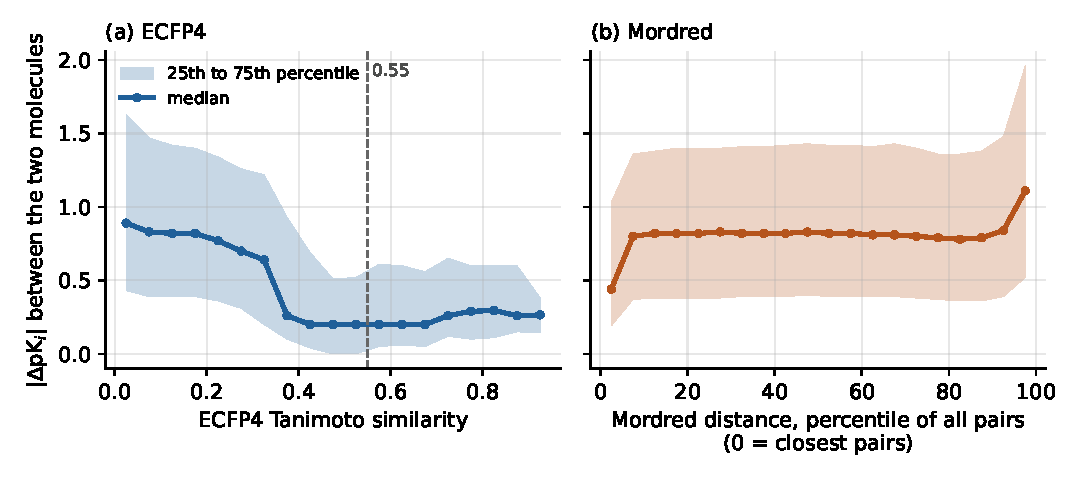
\includegraphics[width=\textwidth,height=0.72\textheight,keepaspectratio]{figures_code_input/herg_ki_pair_distance_vs_dpki.pdf}
\caption[Absolute p$K_i$ difference against pair distance on hERG $K_i$.]{Absolute p$K_i$ difference against distance for all pairs of hERG $K_i$ molecules, with the median in each bin (markers) and the interquartile range (shaded). a) ECFP4 Tanimoto similarity in bins of 0.05 (bins with fewer than 20 pairs omitted), with the activity-cliff threshold of 0.55 dashed. b) Manhattan distance on standardized Mordred features, as a percentile of all pairs.}
\label{fig:flaws:herg_pairs}
\end{figure}


\begin{table}[t]
\centering
\small
\setlength{\tabcolsep}{3.5pt}
\begin{adjustbox}{max width=\textwidth,max totalheight=0.78\textheight}
\begin{tabular}{lrrrrrrrrl}
\toprule
 & & \multicolumn{3}{c}{All pairs} & \multicolumn{3}{c}{Five neighbors} & \multicolumn{2}{c}{Cliffs} \\
\cmidrule(lr){3-5}\cmidrule(lr){6-8}\cmidrule(lr){9-10}
Dataset & Molecules & ECFP4 & Desc. & SMI-TED & ECFP4 & Desc. & SMI-TED & Molecules & Gap \\
\midrule
hERG $K_i$ & 1,412 & 0.06 & 0.07 & 0.09 & 0.72 & 0.72 & 0.69 & 211 & 1.76 p$K_i$ \\
LogD & 5,028 & 0.12 & 0.06 & 0.10 & 0.76 & 0.80 & 0.76 & 731 & 2.90 log \\
Caco-2 & 2,158 & 0.08 & 0.18 & 0.14 & 0.59 & 0.62 & 0.57 & 324 & 1.21 log \\
RLM clearance & 3,053 & 0.02 & 0.07 & 0.04 & 0.36 & 0.49 & 0.46 & 458 & 0.34 log \\
MDR1--MDCK efflux & 2,641 & 0.02 & 0.16 & 0.10 & 0.51 & 0.58 & 0.59 & 397 & 0.20 log \\
HLM clearance & 3,086 & $-0.00$\textsuperscript{\textdagger} & 0.07 & 0.03 & 0.37\textsuperscript{\textdagger} & 0.49 & 0.45 & 462 & 0.27 log \\
QM9 & 9,978 & 0.19 & 0.18 & 0.13 & 0.88 & 0.84 & 0.85 & 1,495 & 0.05 eV \\
\bottomrule
\end{tabular}
\end{adjustbox}
\caption[All-pairs correlation, five-nearest-neighbor prediction and activity cliffs per dataset.]{All-pairs correlation, five-nearest-neighbor prediction and activity cliffs for each dataset. All pairs gives the Spearman correlation between pair distance and absolute label difference, and Five neighbors the Spearman correlation between each label and the mean label of its five nearest neighbors. Cliffs gives the number of cliff molecules and the label gap that defines a cliff. Desc.\ is Mordred, or PDV on Caco-2, and \textsuperscript{\textdagger} marks ECFP4 where it is not a base representation of the dataset.}
\label{tab:flaws:distance_summary}
\end{table}


\begin{table}[t]
\centering
\small
\setlength{\tabcolsep}{4pt}
\begin{adjustbox}{max width=\textwidth,max totalheight=0.78\textheight}
\begin{tabular}{llrrrrrr}
\toprule
 & & \multicolumn{3}{c}{Five-neighbor overlap} & \multicolumn{3}{c}{ECFP4 against MCS} \\
\cmidrule(lr){3-5}\cmidrule(lr){6-8}
Dataset & Desc. & \makecell{ECFP4--\\Desc.} & \makecell{ECFP4--\\SMI-TED} & \makecell{Desc.--\\SMI-TED} & Spearman & Pairs & \makecell{Timed\\out} \\
\midrule
hERG $K_i$ & Mordred & 0.52 & 0.50 & 0.47 & 0.20 & 495 & 5 \\
LogD & Mordred & 0.38 & 0.41 & 0.41 & 0.51 & 494 & 6 \\
Caco-2 & PDV & 0.38 & 0.41 & 0.38 & 0.51 & 492 & 8 \\
RLM clearance & Mordred & 0.15 & 0.21 & 0.18 & 0.28 & 500 & 0 \\
MDR1--MDCK efflux & Mordred & 0.15 & 0.20 & 0.17 & 0.26 & 500 & 0 \\
HLM clearance & Mordred & 0.15 & 0.21 & 0.18 & 0.20 & 500 & 0 \\
QM9 & Mordred & 0.13 & 0.18 & 0.21 & 0.46 & 500 & 0 \\
\bottomrule
\end{tabular}
\end{adjustbox}
\caption[Agreement between representations per dataset.]{Agreement between representations for each dataset. Five-neighbor overlap is the mean fraction of a molecule's five nearest neighbors that two representations share. ECFP4 against MCS gives the Spearman correlation between ECFP4 Tanimoto distance and MCS distance, the number of pairs used, and the number left out because the MCS search timed out.}
\label{tab:flaws:neighbor_overlap}
\end{table}
% ==== END CODE INPUT ====


\subsection{Distance metrics for continuous molecular descriptors}


While binary fingerprints are compared with the Tanimoto coefficient (Chapter~\ref{chap:background}), we need distance metrics for continuous feature vectors. The research in Section~\ref{sec:lnl_motivation} used the following four:

\begin{itemize}
    \item Euclidean ($L_2$): standard geometric distance, $d(x, y) = \sqrt{\sum_i (x_i - y_i)^2}$
    \item Manhattan ($L_1$): sum of absolute differences, $d(x, y) = \sum_i |x_i - y_i|$, more robust to outlier features
    \item Cosine: angle-based, $d(x, y) = 1 - \frac{x \cdot y}{\|x\| \|y\|}$, invariant to magnitude
    \item Mahalanobis: covariance-adjusted distance, $d(x,y)=\sqrt{(x-y)^\top S^{-1}(x-y)}$, where $S$ is the feature covariance estimated on the training molecules \citep{Mahalanobis1936}
\end{itemize}

All features are standardized to zero mean and unit variance prior to distance computation.

% TODO: review, needs manual review -- rewritten 2026-10-08 to match the code: the similarity objective uses Manhattan only (src/kirby/distance_config.py default); Chapter 6 sweeps Manhattan, cosine and Minkowski p=0.5 up to 5,000 molecules, Manhattan and cosine above (tests/experiments/noise/similarity_space.py GROUP_METRICS); Euclidean was cut 2026-10-05; importance weighting was cut from the noise suite but survives in some similarity experiments, so the old weighting sentence was removed here
The later chapters use a different set, chosen after that study. The hybrid search's nearest-neighbor objective (Chapter~\ref{chap:method}) uses Manhattan distance only. Chapter~\ref{chap:similarity} compares Manhattan, cosine and Minkowski distance with $p=0.5$, $d(x,y)=\left(\sum_i |x_i-y_i|^{0.5}\right)^{2}$, on datasets of up to 5,000 molecules, and Manhattan and cosine on larger ones. The Minkowski distance with $p=0.5$ is a dissimilarity rather than a metric, because it breaks the triangle inequality.

\section{Consequences for similarity-based methods}\label{sec:flaws:consequences}

% [CLAUDE 2026-10-09] citation note: Hanser2025 is paywalled; distance-weighted votes are not in its abstract. Lhasa's FLuID_POC code does weight teachers by the 8 nearest neighbours (lhasa/FLuID_POC/preprocessing/FLuID.py ~l.901). Check the paper's Methods before keeping this citation.
We've identified some issues within the representations and similarities computed over them. While this calls into question the predictive limits of QSAR and other structure-based modeling, it also calls into question downstream applications of molecular similarity. Nearest-neighbor methods, where a molecule's neighbors, as measured by similarity, are the inputs to several other processes, are by definition sensitive to the quality of similarity measurements. They are used within other processes like predicting a molecule's activity using its neighbors' labels, detecting outliers, either ACs or noise, defining an applicability domain by distance to the training set \citep{Tropsha2010}, grouping molecules into clusters for data splits \citep{Butina1999}, identifying activity cliffs, and, in federated learning, weighting each site's vote on a molecule by that molecule's distance to the site's own data \citep{Hanser2025}. If this measure of similarity, or equivalently distance, is flawed, then all of these downstream applications will feel the effects of it.

Section~\ref{sec:lnl_motivation} reports the exploratory LNL study, in which the 20 configurations with the lowest retention under noise all relied on a pairwise distance measurement somewhere in their process. Section~\ref{sec:flaws:neighbors} focuses directly on neighbor-based noise detection, the most clear-cut use of similarity. 

% TODO: my confirmatino report was written by me, not you, so wherevery possible, use my original language
% There will be things you need to add, like a quick explanation of the noise metric I'm using (explain it predated auc_norm) and is more strongly correlated with R2 so it's harder to isolate noise, but for the pruposes of this experiment its a good proxy, the main point being the similarity/distance-based methods are broken
% Definitely not nearly as much detail as my confirmation report, I like the detail you have, just try to copy the direct language from my original report more
% Actually no, upon reading it further it's not enough. I'm going to need a table of the methods like I have from the report, and it needs to clearly mark how similarity/distance is used, if at all
% Go through what results the confirmation reoprt lists and I'll see what I want to transfer over, some of these come back in KIRBy (which unfortunately I'm still waiting on results for)
\subsection{Exploratory study of learning with noisy labels}\label{sec:lnl_motivation}

% [OLD TEXT replaced by CODE INPUT below]
% Numerous studies have explored Learning with Noisy Labels (LNL) in the broader context of ML, as well as specifically for QSAR models. \citet{Song2022} provide a comprehensive review of Deep LNL, identifying five main approaches: (i) modifying architectures to better handle noise in training; (ii) employing regularization to reduce overfitting to noise; (iii) adjusting loss functions to be less sensitive to outliers or label flips; (iv) post-processing to adjust the weights for noisy data; and (v) sample selection to select presumably clean data to pre-train. \citet{Cortes2015} examined 12 different algorithms across 12 datasets and 10 noise levels, finding that no single algorithm was overall best at maintaining predictive performance in the presence of noise; certain algorithms perform better or worse at different levels of noise. This is a recurring theme in LNL research: there is no universal solution to handling noise with experimental endpoints.
% There are a wide variety of approaches to LNL, spanning sample selection, meta-learning, curriculum learning, and iterative refinement \citep{Song2022}. Cheminformatics data presents additional challenges in the form of high-dimensional molecular representations and dealing with a wide variety of chemical domains with various similarities and relationships. In this chapter, we explore a set of 12 LNL methods in the context of QSAR modeling. We examine the impact of uncertainty quantification, molecular distance metrics, and alternative loss functions in the hopes of improving performance under label noise. We tested 221 total configurations across LNL methods, loss functions, distance metrics, and molecular representations. Notably, we found that molecular representation choice explains even less variance under LNL methods. We also identified the following LNL techniques which showed promise on the tasks at hand: heteroscedastic GP, curriculum learning, and sample selection methods. The work was meant to connect the representation and uncertainty quantification insights found in Chapter~\ref{chap:robustness} with more classical noise mitigation techniques as a means of determining broader research directions. 
%
% One of the most prominent outcomes was that distance-augmented methods performed significantly worse than ones that did not incorporate any sense of distance or molecular similarity. An ANOVA test was run on the different adapted factors and shows that distance metric usage is the dominant factor in variance in $R^2$.. When ranking the performance of methods, all 20 worst-performing configurations with respect to noise robustness used distance metrics, not a single one achieved both high baseline ($R^2 > 0.6$) and high noise retention ($> 80\%$). This pattern was observed across standard distance types (Euclidean, Manhattan, Cosine, Mahalanobis) and a chemistry-aware metric (Tanimoto coefficient). 
%
% Building upon the exploratory study above, we decided to investigate alternative featurization techniques. There are multiple possible explanations behind the poor performance of distance metrics, first being that a singular molecular representation lacks sufficient information for distance calculations, with and possibly even without noise. These representations all encode different types of molecular information, PDVs encode global molecular properties, ECFPs contain substructure information, and MPNNs such as MHG-GNNs capture 3D structural features. These single sources of data may not be sufficient for robust similarity estimation. Additionally, some of these representations are sparse and contain a large number of features that are not relevant to molecules of a given domain. 
%
% The main issue we identified here is that when a large proportion of dimensions are uninformative, similarity measures become dominated by those uninformative features, causing exponential growth in the number of irrelevant pairwise interactions as dimensionality increases. This is what we sought to address by developing a representation with informative features and low dimensionality. We do so by creating a budget-constrained hybrid representation, which takes high-importance features from a variety of sources. These hybrid representations concatenate the top-ranked features by importance from a selection of base representations. 
% ==== CODE INPUT: new, needs review ====
% Transferred from the confirmation report (paper.tex, Chapter 4 "Exploring techniques for learning with noisy labels for QSAR", and the opening of Chapter 5), shortened, with the "Change:" bullets applied.
% TODO: Ch3 update -- re-check the Chapter 3 results quoted in this paragraph against the updated chapter.
% TODO: review, needs manual review
This section reuses an exploratory study of LNL carried out earlier in this project. In Chapter~\ref{chap:robustness}, model family explained the largest share of the variance in robustness to label noise, and representation at most 11.2\%, so we asked whether training methods built for noisy labels improve robustness, and whether the representation still matters under them.

LNL methods and the five groups of \citet{Song2022} are described in Section~\ref{sec:lnl_background}, and such methods have been studied across machine learning, including QSAR. Most LNL methods were built for image classification with flipped labels \citep{Song2022}, so they do not transfer automatically to continuous labels.

% TODO: the exploratory study's sigma is not stated to be in the units of the Chapter 2 noise level (a fraction of the clean training-label standard deviation, Equation eq:dose_matching). Check the confirmation-report code; if it is, say so here with a pointer to Section sec:noise_injection.
% TODO: review, needs manual review
The study tested 12 LNL methods on the QM9 HOMO--LUMO gap (10,000 molecules, scaffold splits), adding Gaussian noise with $\sigma$ from 0 to 1.0 in steps of 0.1 to the training labels only. The representations were ECFP4, Sort \& Slice \citep{sns}, PDV, canonical SMILES and randomized SMILES. Depending on the method, a configuration could add the model's own uncertainty, a distance between molecules (Tanimoto, Euclidean, Manhattan, cosine or Mahalanobis), an alternative GP kernel or an alternative loss function, giving 221 configurations. Four methods, small-loss selection, confident learning, distance-based selection and multistage cleaning, remove suspected molecules and retrain. These are noise mitigation methods; the other eight are noise-robust training methods.

% TODO: the study says 'all 20 worst-performing configurations ... used distance metrics, not a single one achieved both high baseline (R^2 > 0.6) and high noise retention (> 80%)'. It is ambiguous whether 'not a single one' means the 20 worst or every configuration with a distance. This sentence reads it as every configuration with a distance.
% TODO: review, needs manual review
We measured noise robustness by retention, $R^2$ under noise divided by $R^2$ with clean labels, as a percentage, which is the retention ratio of Chapter~\ref{chap:robustness} (``Evaluation''). Methods that used a distance did worse than those that did not, and in an analysis of variance over the adapted components, whether a distance was used explained the most variance in $R^2$. All 20 configurations with the lowest retention used a distance, and none with a distance reached both a clean $R^2$ above 0.6 and a retention above 80\%.

% [CLAUDE 2026-10-09] citation fix: liu2020 (Liu, Ong & Cai) uses a second GP for the noise; the thesis's heteroscedastic GP is a GP plus a small network (closer to Kersting 2007). lnl_methods.py ranks by own loss, which is self-paced learning (Kumar 2010). Check that the exploratory study ran this code.
The methods that held up estimate noise from the model's own loss or uncertainty. DivideMix \citep{li2020dividemix} retained the most, 86.7\% (standard deviation 0.4\%), followed by small-loss selection \citep{Han2018} at 84.2\% (2.1\%) and the uncertainty curriculum, which orders molecules by the model's own loss \citep{Bengio2009, kumar2010selfpaced}, at 82.7\% (3.5\%). The heteroscedastic GP, a GP whose noise is predicted per molecule by a second model \citep{kersting2007most}, retained 79.0\%, averaged over 15 configurations, with $R^2$ of 0.71 on clean labels and 0.56 at $\sigma = 0.6$, where its retention was measured. The exploratory study does not record this noise level for the other methods. Regularization alone retained less, 73.0\% for Mixup and 74.0\% for sharpness-aware minimization. Under these methods, the choice of representation explained even less variance than in Chapter~\ref{chap:robustness}.

% TODO [2026-10-09]: HOW THIS STUDY COMPARES WITH THE LATER SURVEY. Verified in session against
%   ~/Downloads/Confirmation_Report/paper.tex:680-712 and src/kirby/utils/lnl_methods.py:2309-2326.
%   (1) SAME TWELVE METHODS, name for name: meta weight net, small-loss selection, confident
%   learning, distance-based selection, MentorNet, uncertainty curriculum, DivideMix, multistage
%   cleaning, early learning, contrast-to-divide, heteroscedastic GP, evidential kernel.
%   (2) NOT THE SAME CODE. The KIRBy header says "12 methods adapted from the confirmation report
%   LNL survey", so the later survey is a reimplementation. Do not write that it re-ran this
%   study; write that it ran the same twelve methods.
%   (3) "repeats the question" IN THE SENTENCE BELOW IS TOO STRONG, and the cross-reference is
%   stale. The noise work is now its own chapter, not the similarity chapter, so
%   \ref{chap:similarity} needs changing. The later survey shares NO DATASET with this study: it
%   runs on Caco-2, LogD, hERG, hERG Ki, binding free energy, CDR flexibility and three Ginkgo
%   developability sets, and not on QM9. Say that explicitly.
%   (4) IT IS WIDER IN FOUR WAYS: nine datasets instead of one; six damage kinds plus six
%   label-flip kinds instead of Gaussian alone; single representations AND hybrids instead of five
%   single representations; and each method scored against the plain network on the same damaged
%   labels in the same feature space, rather than methods ranked against each other by retention.
%   (5) IT IS NARROWER IN ONE WAY, AND THIS IS WHY THIS SECTION CANNOT BE CUT. The 221
%   configurations here come from crossing the twelve methods with four optional components:
%   uncertainty, a molecular distance, an alternative kernel and an alternative loss function. The
%   later survey sweeps none of the four (n09_lnl_survey.py:102-123 sweeps methods, five feature
%   spaces, damage kinds, levels and three noise draws; only distance-based selection keeps a
%   neighbour sweep). So the analysis of variance on the distance axis has no counterpart later and
%   cannot be reproduced from those runs. This section holds the only measurement of it.
%   (6) WHERE THEY AGREE: on binding free energy, the hardest dataset in the later survey, the
%   heteroscedastic GP is the only method that passes on the labels as delivered and DivideMix the
%   only one that passes under injected damage, which keeps both in the role they have here.
%   (7) ONE REVERSAL, to state plainly: distance-based selection is the worst of the twelve here,
%   and in the later survey it is the ONLY one of the twelve that passes on hERG under label flips
%   at a rate of 0.1.
%   (8) WHAT THIS STUDY COULD NOT SEE: in the later survey, on all nine datasets, the method that
%   scores best on a hybrid is not the method that scores best on either single representation. So
%   the ranking of these methods is a property of the feature space, not of the method.
% TODO: review, needs manual review
The study used one dataset, one property and one noise condition (Gaussian noise on every training label), and Chapter~\ref{chap:similarity} repeats the question on more datasets and under other noise conditions (Section~\ref{sec:noise_injection}). It also added the distance step to methods designed without one, so poor adaptation is an alternative explanation.

The distances may have failed for two reasons, which the evidence here does not separate. First, a single representation may lack the information a distance needs, with and possibly even without noise. PDVs encode global molecular properties, ECFP4 contains substructure information and MHG-GNNs encode the molecular graph \citep{kishimoto2023}, and any one of these sources alone may not be sufficient for robust similarity estimation. Second, some representations are sparse, with many features irrelevant to the molecules of a given dataset (Section~\ref{sec:flaws:similarity}). We sought to address the second with the adaptive hybrid representation (Chapter~\ref{chap:method}), which concatenates the top-ranked features by importance from several base representations.
% ==== END CODE INPUT ====


\subsection{Noise detection by neighbors}\label{sec:flaws:neighbors} % CODE INPUT: label added, needs review
% [notes moved to thesis_notes_moved.md]

% [OLD TEXT replaced by CODE INPUT below]
% Overall, we see in agreement with conclusions of Section~\ref{sec:lnl_motivation} on the use of distance metrics in LNL methods, the concept of using a sample's neighbors to determine it's ground truth is flawed. It is likely all labels are too uniformly noisy for a methodology like this. Uncertainty-based methods show potential at lower noise, but their estimation performance degrades with higher noise. Sampling weighting methods generally proved effective, and one estimator using exponential sample weighting produced very strong recovery across both noise levels.
%
% Hybrid representations had mixed results. For sample removal, hybrids showed advantages at high noise, but struggled at low noise. They showed consistently positive recovery rates for neighbor-based estimation, which roughly falls in line with the idea that a low-dimension, high-quality information representation benefits neighbor-based reasoning. The feature budget in this experiment was restricted to 50-100 features, which may limit its advantages. This range was successful at standard molecular property prediction, but potentially not for certain noise mitigation or estimation tasks. Distance-based methods remain challenging under Gaussian noise regardless of representation, suggesting the core issue is the noise distribution rather than representation quality alone. This merits an investigation into mitigation of noise from other distributions or noise injection strategies.
% ==== CODE INPUT: new, needs review ====
% Transferred from the confirmation report (paper.tex, Chapter 5 "Noise Estimation" results, lines 1028-1146), shortened, with the "Change:" bullets applied.
Neighbor-based noise detection treats a label far from its neighbors' labels as probably wrong, an idea that goes back to editing nearest-neighbor training sets \citep{Wilson1972}. The wider literature on filtering noisy labels concerns classification \citep{Brodley1999, frenay2014classification}. \citet{Martin2021} adapt fourteen classification noise filters to regression, seven of them nearest-neighbor filters that use the neighbors' mean label. They find that the filters improve regression methods on 20 general regression benchmarks with injected label noise, none of them QSAR datasets.
% Source needed (from her NOTES, still open): a QSAR source for removing or down-weighting a molecule because its label disagrees with its nearest neighbors' labels.
The neighbor-based noise scores, sample removal, sample weighting, label smoothing and the recovery rate are defined in Chapter~\ref{chap:similarity}, ``Noise mitigation methods''.

The method needs a distance that picks the right neighbors, and neighbors with clean labels. Earlier sections of this chapter argue that the first condition fails, and the second fails whenever noise is spread over the whole training set. A large gap from the neighbors' labels can mean a noisy label, a noisy neighbor or the wrong neighbors, and the score cannot tell which. Activity cliffs also look like noise to such a detector (Chapter~\ref{chap:background}, ``Molecular similarity and activity cliffs'').

The exploratory study also used neighbors to clean labels, on 5,000 randomly chosen QM9 molecules (HOMO--LUMO gap, scaffold split) with Gaussian noise on the training labels at $\sigma = 0.3$ and $\sigma = 0.6$. Each cleaning method was judged by retraining a random forest on ECFP4 with clean, noisy and cleaned labels, giving the recovery rate, the share of the $R^2$ lost to noise that cleaning recovers (Equation~\ref{eq:recovery}). Neighbor-based scores compared each label with those of the molecule's $k$ nearest training molecules under Euclidean, Manhattan or cosine distance. Table~\ref{tab:code_input_neighbor_recovery} holds only the configurations built on a single representation; those built on an early hybrid are described below. This study is separate from the sample-removal study of Chapter~\ref{chap:similarity}.

With the neighbor-based scores used as sample weights at strength $\alpha = 0.1$, mean recovery was negative for every representation at both noise levels (Table~\ref{tab:code_input_neighbor_recovery}). Of all 860 cleaning configurations, 8 had positive recovery at both noise levels; 6 of these used a single representation, and 4 of those 6 were neighbor-based. Label smoothing toward neighbor or model estimates gave positive recovery in 5.0\% of configurations at $\sigma = 0.3$ and 0.8\% at $\sigma = 0.6$. Mean recovery was negative at every weighting and smoothing strength tried, from 0.1 to 0.7.

\begin{table}[htbp]
\centering
\begin{adjustbox}{max width=\textwidth,max totalheight=0.78\textheight}
\begin{tabular}{lcccc}
\toprule
 & \multicolumn{2}{c}{Mean recovery (\%)} & \multicolumn{2}{c}{Positive (\% of configurations)} \\
\cmidrule(lr){2-3}\cmidrule(lr){4-5}
Representation & $\sigma = 0.3$ & $\sigma = 0.6$ & $\sigma = 0.3$ & $\sigma = 0.6$ \\
\midrule
ECFP4   & $-3.0$ & $-7.3$ & 33.3 & 16.7 \\
PDV     & $-2.4$ & $-3.4$ & 50.0 & 27.8 \\
MHG-GNN & $-0.1$ & $-7.2$ & 38.9 & 5.6 \\
\bottomrule
\end{tabular}
\end{adjustbox}
\caption[Recovery with neighbor-based sample weights by representation.]{Recovery rate in $R^2$ on the QM9 HOMO--LUMO gap when neighbor-based noise scores are used as sample weights, for each representation used to find the neighbors, at two levels $\sigma$ of Gaussian label noise. Recovery is the share of the $R^2$ lost to noise that cleaning regains, so negative values mean cleaning made the model worse. Positive is the share of configurations with recovery above zero.}
\label{tab:code_input_neighbor_recovery}
\end{table}

Judging a label by its neighbors usually made the model worse and rarely helped at both noise levels, but it did not always fail. The best configuration at $\sigma = 0.6$ was neighbor-based (PDV, Euclidean distance, local variance ratio score) and recovered +17.2\%. Because noise was added to every training label, the neighbors' labels are noisy too; the exploratory study gave this as the reason label smoothing failed.

Uncertainty-based methods, which use no neighbors, showed potential at lower noise but degraded at higher noise. Sample weighting did better than label smoothing but usually still hurt, with positive recovery in 14.2\% of configurations at $\sigma = 0.3$ and 4.7\% at $\sigma = 0.6$, and mean recoveries of $-22.9\%$ and $-20.9\%$.

% TODO: review, needs manual review
The study also found neighbors in an early hybrid of 100 PDV and MHG-GNN features, built by greedy forward selection, which is no longer part of the method. Its mean recovery with neighbor-based scores was $-0.9\%$ at $\sigma = 0.3$ and $-3.0\%$ at $\sigma = 0.6$, with 44.4\% and 27.8\% of configurations positive. Chapter~\ref{chap:similarity} repeats the measurement in a hybrid and under noise conditions other than Gaussian.
% ==== END CODE INPUT ====

\section{Conclusions}
% [notes moved to thesis_notes_moved.md]
% ==== CODE INPUT: new, needs review ====
% Sample conclusion following NOTES Paragraphs 1-6 and the Table. No new evidence.
% Every number is copied from another CODE INPUT fragment of this chapter:
%   Paragraph 1: out/constant.tex (constant/constant_counts.json) and out/ties.tex (ties/ties_results.json).
%   Paragraph 2: out/distance.tex (distance/results_all.json).
% If those fragments change, these numbers must change with them.

On a single dataset, often very little of a standard representation varies. On hERG $K_i$, 1,815 of the 2,048 ECFP4 features take one value in at least 95\% of the 1,412 molecules (Section~\ref{sec:flaws:constant}). Several representations also give different molecules, mostly stereoisomers, the same feature vector, and no model can separate those molecules, whatever their labels. ECFP4 gives 56 of the 1,412 hERG $K_i$ molecules a vector shared with another molecule, all of them stereoisomers (``Molecules with identical feature vectors'').

A distance sums over every feature, so when only a few features matter for the property, the rest dominate the sum (Section~\ref{sec:flaws:similarity}). Across 70 combinations of dataset and representation, the Spearman correlation between pair distance and label difference was below 0.10 in 44. % CHECK: NOTES say keep the all-pairs vs nearest-neighbor contrast only if the full runs support it. The numbers below come from distance.tex, computed on the saved features, not from the full runs.
Predicting each label from its five nearest neighbors gave a higher Spearman correlation in all 70, so the useful information sits in a few close pairs rather than in the distance as a whole.

% TODO: review, needs manual review
In the exploratory LNL study, configurations that used a distance did worst under label noise (Section~\ref{sec:lnl_motivation}), and judging a label by its neighbors' labels usually made the model worse (Section~\ref{sec:flaws:neighbors}). It did not always fail, since one neighbor-based configuration gave the best recovery at the higher noise level. That noise was Gaussian on every training label, so each molecule's neighbors were noisy too; Chapter~\ref{chap:similarity} turns to the other noise conditions of Chapter~\ref{chap:background}.

A representation that avoids these flaws would need five properties (Table~\ref{tab:flaws:requirements}). Its features would be chosen for the task, using only each fold's training labels. It would be compact, dropping features that do not vary or do not matter, with the number kept searched rather than fixed. It would draw on several representations, since each misses information the others capture; plain concatenation does this but is not compact (Chapter~\ref{chap:method}, ``Combining representations''). It would work both as a model input and as a space for similarity. Finally, it would be traceable: each chosen feature leads back to its representation and can be read chemically wherever the base feature can.

Feature selection cannot fix every flaw. Molecules identical in every base representation stay identical in the hybrid, and a selected hashed bit still merges every substructure folded into it. Selection also needs enough labeled molecules to estimate which features matter.

% TODO: review, needs manual review
These flaws are where the thesis began (Chapter~\ref{chap:intro}), and Chapter~\ref{chap:method} builds the method they led to, the adaptive hybrid representation. The settings that method searches over are listed in Chapter~\ref{chap:method}, ``The search space''.



\begin{table}[htbp]
\centering
\small
\begin{adjustbox}{max width=\textwidth,max totalheight=0.78\textheight}
\begin{tabular}{P{0.34\textwidth}P{0.30\textwidth}P{0.28\textwidth}}
\toprule
Flaw (where shown) & Requirement & Where handled \\
\midrule
Features that do not vary (``Constant and near-constant features'') & Features chosen for the task, within a budget & ``Feature importance scoring'' \\
Molecules merged into one vector (``Molecules with identical feature vectors'') & Features drawn from several representations & ``Combining representations'' \\
Distance dominated by irrelevant features (``Flaws in similarity and other pairwise computations'') & Compact, with the number of features searched & ``The search space'' \\
Poor performance of neighbor-based methods (``Consequences for similarity-based methods'') & Usable as a space for similarity & ``Similarity in a hybrid'' (Chapter~\ref{chap:similarity}) \\
% TODO: review, needs manual review
Features that are hard to read chemically (``Flaws in standard representations'') & Traceable, so that each chosen feature leads back to its representation and can be read chemically wherever the base feature can & ``Blueprints and their chemical interpretation'' \\
\bottomrule
\end{tabular}
\end{adjustbox}
\caption[Flaws of standard representations and similarity, and the requirement each sets.]{Flaws of standard representations and similarity, the requirement each sets for a representation, and where the requirement is addressed, in Chapter~\ref{chap:method} unless stated.}
\label{tab:flaws:requirements}
\end{table}
% ==== END CODE INPUT ====


\chapter{Building Adaptive Hybrid Representations}\label{chap:method}
% ---- TAKEAWAYS ----
% - Joining whole representations adds their irrelevant features along with the useful ones. The hybrid combines and filters at once.
% - A hybrid is an input, not a model: up to a budget of features, selected from several base representations by a search for one dataset and one downstream model.
% - No setting of the search wins on every dataset or model, so importance method, allocation method, representation count, internal evaluator, budget and downstream model are all searched.
% - Every selected feature traces back to its representation, so a blueprint can show a chemist which substructures and descriptors the model relies on.
% - The method needs only a supervised label and several vector representations of the same samples, so it carries over to antibodies, reactions, nucleotides and tumor data.
% - Where one representation already dominates, the hybrid should show little gain. The search is costly and must be rerun when the data, representations or model change.
% ---- END TAKEAWAYS ----


\section{Introduction}

So far, Chapter~\ref{chap:flaws} explained how the standard methods of estimating molecular similarity, or conversely distance are flawed and potentially break the SPP. Specifically, the representaions used in these similarity calculationsc contains irrelevant features that either do not vary or more generally do not pertain to the prediction task at hand. This chapter explores a solution. With the understanding that each representation contains a set of features which contain a certain type of information about that data. We aim to select the most informative features across a larger set of representations, while filtering out the irrelevant ones. We create an adaptive hybrid representation, a set of features bounded by a budget that is selected from several base representations by a search using one dataset and downstream model. The goal is to select a set of features that is customized for a given model and prediction task. As discussed in Chapter~\ref{chap:robustness}, performance can vary signficantly across datasets and models. Rather than hope the features you give a model will be useful, this process let's you prescreen them. 


In this chapter we build the adaptive hybrid representation, referred to as the hybrid representation, first reporting on when and why it helps. The questions this chapter and Chapter~\ref{chap:similarity} address are set out in Chapter~\ref{chap:intro} (Section~\ref{sec:intro:hybrid_questions}). This chapter measures predictive performance under both standard labels and labels with injected artificial noise. Distance meseasures between hybrids, noise detection and LNL are covered in Chapter~\ref{chap:similarity}.


\subsection{Combining representations}
% - TODO(lit): read the Turkina2025 full text for whether a fixed number of bits is kept per fingerprint, or all bits are ranked together.

% TODO: ensure consistent use of embeddings langauge
% [CLAUDE 2026-10-09] citation fix: Deng2023 says 'many datasets', not the majority.
% [CLAUDE 2026-10-09] citation fix: Mayr2018's SmilesLSTM is a recurrent network trained on SMILES, not language-model embeddings.
% [CLAUDE 2026-10-09] citation fix: Kenlay2024 supports this only through its expression vs binding result; Schmirler2024 does not state it (removed); ElNahhas2025 finds CONCH best overall, so 'dominates' was too strong.
Not every molecular representation is equal. In fact, they hold very different types of information. RDKit2D descriptors matched or outperformed features derived from embedded GNNs and pretrained language models on many datasets across 62,820 models on a variety of molecular property prediction benchmarks \citep{Deng2023}. Descriptor-based models held 73\% of top-three positions on 11 benchmarks \citep{Jiang2021}. In 1,310 ChEMBL assays, feedforward networks on ECFP fingerprints outperformed graph convolutions and recurrent networks trained on SMILES \citep{Mayr2018}. We know that the choice of representation matters, as is discussed in Chapter~\ref{chap:robustness}, yet this choice is usually decided by trial-and-error. Beyond just molecules, general protein language models predict antibody expression better than antibody-specific ones, while the antibody-specific models are better on binding \citep{Kenlay2024}, and no pathology foundation model is best on every clinical task \citep{ElNahhas2025}. We turn our attention to combining features from these different representations. 

Most research in this field relies on a single representation, and few combine features from different representations beyond concatenation. One of the reasons just pooling features from different representations together doesn't work is dimensionality. If you add a standard ECFP4 ($d=2,048$) with Morderd descriptors ($d=1,613$) and an MHG-GNN embedding ($d=1,024$), you end up with 4,685 features, which is far too many considering many datasets from experimental assays contain only a few hundred labeled samples. With such ratios, more features mean weaker predictions \citep{Hughes1968, Bellman1961}. Therefore, we consider ways of combining representations. 

% TODO: I'm pretty sure I'm doing late fusion but calling it ensembling, make sure its appropriately named below
% [CLAUDE 2026-10-09] citation fix: Steyaert2023 is a review that describes late fusion; MOGONET (Wang2021) fuses predictions in label space, which is late, not intermediate, fusion.
The most straightforward method of combining representations is concatenation. This however degrades wiht non-homogenous feature sets and obscures which reprsentation is responsible for the score \citep{Stahlschmidt2022}. \citet{Deng2023} found that appending RDKit2D descriptors to GROVER lowered RMSE on 9 of 24 datasets tested. Late fusion trains one model per source and aggregates the predictions \citep{Steyaert2023}. MOGONET is of this kind, combining per-source predictions in label space \citep{Wang2021}. While this is effective, it loses interactions between the source representations, an issue which is addresed by intermediate fusion, for example cross-attention between sources \citep{Beaude2025}. Multiple kernel learning does this with kernels rather than whole models \citep{Gonen2011, Cichonska2018}, and produces no interpretable feature sets. \citet{Laufktter2019} found that combining bioactivity-based fingerprints with structure-based ones like ECFP4 improved both predictive performance and scaffold-hopping. Similarly, \citet{Turkina2025} combined features from six non-hashed fingerprints with feature importance scores and showed that the additional features consistently improved predictive accuracy over the original fingerprints across a range of models. Most of this work involves limitation combinations, adding together standard fingerprints and linear representations \citep{Xie2020, Laufktter2019}. Although the features derived from embeddings are not as conceptually-straightforward, they contain another axis of information. 

Beyond simply combining features, there are a range of other methods that handle training on multiple representatinos or excessive feature sets. Ensembling fits one model per representation and aggregats their predictions, essentially combining the information carried by each representation after tarining rather than before. Consensus QSAR works this way \citep{Valsecchi2020}. One drawback is that no model in an ensemble sees features from other representations so their interaction is never measure, and every representation and every model must be computed for each new 

When you want to select filter a feature set for the most important to the prediction task, you can use a dimensionality reduction technique or feature selection methodology. Principal component analysis (PCA) uses linear combinations of the original features, ordered by the variance they explain \citep{Jolliffe2016}. Their combined features are dependant on the original feature units unless each feature is z-scored first which matters when data from different modalities like fingerprint bits, descriptors and embeddings are joined \citep{Jolliffe2016}. PCA never sees the labels, and components with small variance can still be important in prediction \citep{Jolliffe1982}. Partial least squares (PLS), the supervised counterpart in chemometrics, builds components that covary with the property \citep{Wold2001}. Neither gives components that can be traced to one substructure, descriptor or representation, making them difficult to interpret.

Feature selection keeps a subset of the original features, unlike PCA or PLS which builds new ones. Of its three families \citep{Guyon2003}, filter methods score features against the labels before any model is fitted, as minimum-redundancy maximum-relevance selection (mRMR) ranks features by their mutual information, defined as the label minus its redundancy with already-chosen features \citep{Peng2005}. Wrapper methods score subsets of features by fitting the model \citep{Kohavi1997}. Embedded methods select features while the model is fitted, as the does lasso \citep{Tibshirani1996}. Recursive feature elimination repeatedly fits a model and drops the lowest-ranked features \citep{Guyon2002}.

% [CLAUDE 2026-10-09] citation fix: Sort & Slice and the overfitting remark are in the Sort & Slice paper (key sns), not the PhD thesis (Dablander2024).
When selecting features, the question is not only what features are most important, but also, what features does the model prefer? One of the ways to answer this is to consider how many features relative to the size of a dataset a given model works best with. Distance-based models such as $k$-nearest neighbors (kNN) and SVM use every feature in every distance computation (Chapter~\ref{chap:flaws}), whereas tree ensembles choose one feature per split and can essentially ignore irrelevant ones. \citet{sns}, who created a substructure-based fingerprint called Sort \& Slice, suggest that using labels to select features may result in overfitting. Table~\ref{tab:hybrid_alternatives} compares these alternatives with the adaptive hybrid methodology developed in this thesis. 

\begin{table}[htbp]
\centering
\small
\setlength{\tabcolsep}{3pt}
\begin{adjustbox}{max width=\textwidth,max totalheight=0.78\textheight}
\begin{tabular}{P{4.2cm}P{2.3cm}P{2.1cm}P{2.3cm}P{2.6cm}}
\toprule
Method & Uses the labels & Keeps original features & Several representations & Retrain to add one \\
\midrule
Concatenation \citep{Stahlschmidt2022} & no & yes & yes & yes \\
% [CLAUDE 2026-10-09] citation fix: MOGONET (Wang2021) moved from intermediate to late fusion; intermediate fusion now cites Beaude2025 (cross-attention).
Late fusion and ensembling \citep{Steyaert2023, Valsecchi2020, Wang2021} & only if pooling weights are learned & yes & no & no, one more model \\
Intermediate fusion \citep{Beaude2025} & yes & no & yes & yes \\
Multiple kernel learning \citep{Gonen2011, Cichonska2018} & yes & no, kernels only & yes & yes \\
PCA and PLS \citep{Jolliffe2016, Wold2001} & PCA no, PLS yes & no & yes, on a concatenation & yes \\
Flat feature selection \citep{Guyon2003} & yes & yes & yes, on a concatenation & yes \\
Group lasso \citep{Yuan2006} & yes & yes, whole groups & yes & yes \\
Adaptive hybrid representation & yes & yes & yes & search rerun, method unchanged \\
\bottomrule
\end{tabular}
\end{adjustbox}
% TODO: review, needs manual review
\caption[Methods for combining or reducing representations.]{Methods for combining or reducing representations, compared by whether they use the labels, keep the original features, let one model see several representations, and must refit to add a representation.}
\label{tab:hybrid_alternatives}
\end{table}

\subsection{The adaptive hybrid representation}

The task of selecting the best features and combining them from a set of representations and combining them is not simple. How do you measure what features are ``best''? Are these features ``best'' relative to the representation they came from or to the whole pool of features? Should you select more features from repesentations that seem to have more signal to begin with, or take a set number of featurs from every representaton? How many base reprsentations should you select features from? How many features should you select? When scoring potential combinatinos of featurse, what type of evaluator should you use? 

In a dream world, there would be a single answer to each one of these questions that applies to every dataset. Unfortunately we live in reality, and as I discovered, the answer to every single one of these questions is ``depends on the data.'' The task of selecting the best features then became a search space optimisation challenge. The question actually became for a given prediction task, defined by the dataset, prediction target, and model, what is the best methodology for selecting features? The hybrid search does not output just a list of features, rather it outputs an ideal search configuration to find features for your data. It tells you how to score features (feature importance score), what rules you should use to select them (allocation method), how to score potential hybrid feature combinations (internal evaluator). In this research, I run this hybrid search multiple times across different maximum number of features (budgets), number of input representations, and models (downstream evaluators) on each dataset. While it is not formal ``training'' in the ML sense, the hybrid search is essentially a feature selection method that is fit on the training data. The representations used in this thesis are listed in Tables~\ref{tab:reps_smallmol}, \ref{tab:reps_reactions}, \ref{tab:reps_antibodies}, \ref{tab:reps_nucleotides} and~\ref{tab:reps_tcga}.

Formally, an adaptive hybrid representation is a set of fixed number of features, capped at a fixed budget, selected from several base representations of the same molecules. The output of a hybrid search is itself a feature selection method that when run on the given dataset, produces the hybrid repesentation. This search is run on a single datast and downstream model, and the resulting hybrid differs by model, dataset, and even split. Its intended use case is when there are multiple base representations that describe different aspects of a molecule, and you want to combine these different features for a single training task. The hybrid ranks features by a fitted model's importance scores, as embedded methods do, and keeps a fixed number of the top-ranked ones, as a filter does. Classical methods treat all features as one flat list. The nearest classical relative, the group lasso, keeps or drops predefined groups of variables whole \citep{Yuan2006}, whereas the hybrid splits the budget among representations (Section~\ref{sec:method:allocation}). Because only original features are kept, each traces back to one representation, which makes blueprints possible.


\subsection{Blueprints and their chemical interpretation}

As explained above, the adaptive hybrid representation relies on a search. A completed search is saved as a blueprint, which records the settings needed to select the features that make the hybrid representation. Because each selected feature traces back to its original base representation and relative importance rank, the search can tell you about your own prediction task. The best configuration is saved for each downstream model and budget, giving one blueprint per pair, allowing us to compare blueprints and see if different models prefer different features. 

Depending on the origin of the feature, some are chemically interpretable. By definition, the PDV contains values that relate back to chemical propertie like molecular weight or logP. An ECFP4 bit can be shown as the atom environment that sets it, and a MACCS key stands for a known substructure. Beyond small molecules, the readable unit of an antibody is a sequence position and its residue, and for gene expression a named gene set, such as a pathway or a chromosome arm. This feature-level explainability fails when features are derived from learned embeddings. That will only tell you if the learned embedding itself is useful as a representation, but nothing about the selected feature. 

While a set of thousands of features may seem overwhelming and irrelevant, identifying substructures or descriptors that recur among the selected features can point to parts of the molecule that may be involved in binding or activity. If the selected featues make sense chemically for that endpoint, it's a good sign that the selection mechanism is finding real signal instead of fitting nose. Conversely, if the hybrid search is done over a range of budgets or models, and the blueprints are showing a vastly different set of features, that may be an indication that the features at hand are struggling to provide information about the prediction task. A predictor that scores proposed molecules in generative design \citep{Olivecrona2017} could also take a hybrid as input, which we leave to future work.

\subsection{Antibodies and beyond}

The hybrid search is a generalised search that takes in multiple feature matrices fro the same samples and a supervised prediction task, and outputs a set of feature selection method that produces a filtered set of features from those original vectors. The default search objective scores prediction only, meaning the methodology applies to tabular tasks or cases where you have different measurements of the same inputs. Although this was developed with small molecules and QSAR modelling in mind, it is by no means limited to that use case. While there are some functionalities in this research that are tailored to chemical tasks, such as blueprint mappings features back to their chemical interpretations and the use of nearest-neighbor objectives Chapter~\ref{chap:similarity} to aid in the computation of molecular similarity, the core functionality of the hybrid process is domain-independent.

% TODO: review, needs manual review -- rephrased from your TODO "my phrasing needs work here"; the result is still needed
One caveat concerns sparse representations such as one-hot encoded sequences. Each of their features is set in only a few samples, so each scores low importance on its own. Such encodings are usually passed to a network that learns a representation from them, but they can also be used directly. Here, the one-hot encoding is a base representation on nanobody thermostability, and the blocks substitution matrix (BLOSUM) encoding on humanness and trastuzumab--HER2 binding. One-hot was among the selected representations on \textbf{[RESULT NEEDED: antibody datasets where one-hot was selected, with score]}.

% TODO: come back and edit final list of datasets
While this setup was initially intended for small molecules, we extend this research to antimodies. Four antibody dataset are used in this chapter: Koenig expression, nanobody thermostability, humanness and trastuzumab--HER2 binding (Table~\ref{tab:datasets}). Reactions (two Buchwald--Hartwig yield datasets) and nucleotide sequences (the H3K4me3 histone-mark and TATA promoter tasks, Table~\ref{tab:reps_nucleotides}) are used to test applications of this framework in entirely separate domains.  

Another caveat of this setup is that the hybrid can help only on datasets with enough samples (see Section~\ref{sec:method:limitations}) and with base representations whose features carry importance. When all the representations score poorly, there are not enough useful features to pull from. Additionally, if there is only a single base representation that carries signal, there is nothing for the hybrid to improve upon, which is demonstrated in Section~\ref{sec:method:results_single}.

\section{Methods: the hybrid search}

Figure~\ref{fig:hybrid_search_space} outlines the hybrid search.

\begin{figure}[!htbp]
    \centering
    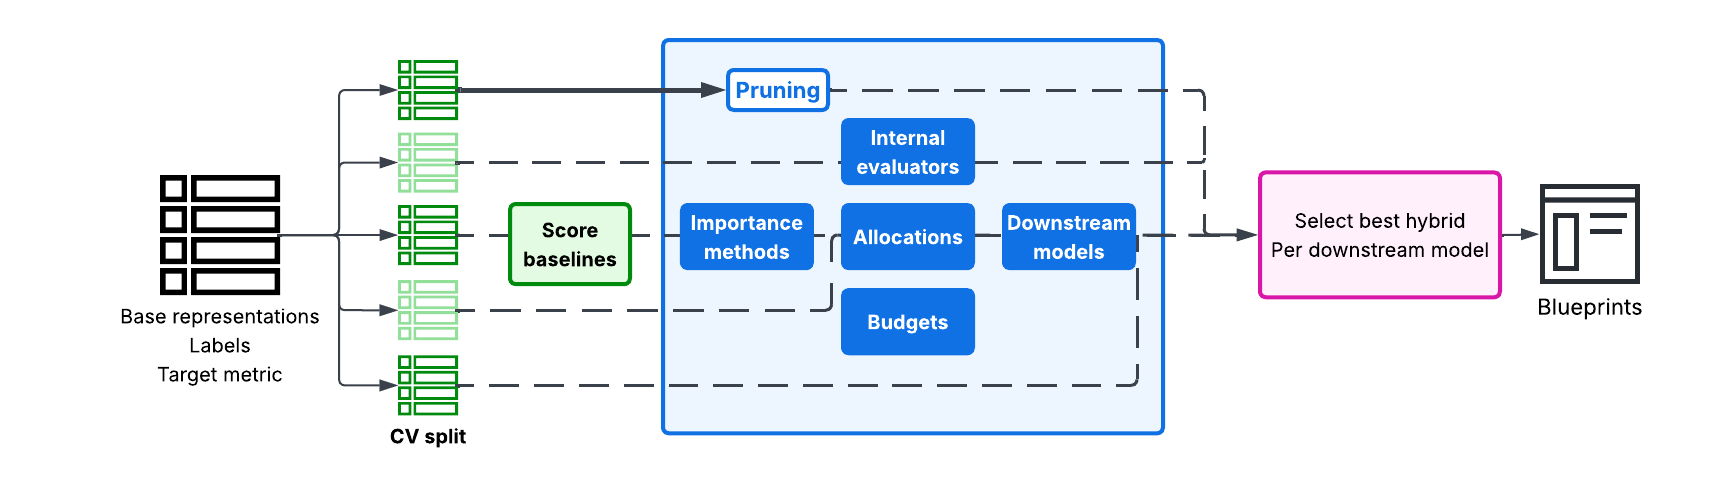
\includegraphics[width=\textwidth,height=0.72\textheight,keepaspectratio]{figures_code_input/hybrid_search_space.png}
    \caption[Schematic overview of the hybrid search.]{Schematic overview of the hybrid search. The inputs (left) are split into five cross-validation folds, and the single representations are scored as baselines. Each fold is searched over importance methods, allocation methods, budgets, internal evaluators and downstream models (center). The best hybrid for each downstream model is stored as a blueprint (right).}
    \label{fig:hybrid_search_space}
\end{figure}


\subsection{From base representations to a hybrid}\label{sec:method:build}

The input to the search is $K$ frozen representation matrices $\mathbf{X}^{(k)} \in \mathbb{R}^{n\times d_k}$, $k = 1, \dots, K$, for the same $n$ samples, whose widths $d_k$ range from tens to thousands of features, as well as a label vector $\mathbf{y}$, one group label per sample for cross-validation (for example, its scaffold group), the evaluation metric, the task type, one or more downstream models and a list of budgets. It returns a hybrid of at most $B$ features before any augmentation features added outside the budget (Section~\ref{sec:method:augmentation}), where the budget $B$ is a maximum rather than a target, and a blueprint that records the settings necessary to rebuild the hybrid representation on another set of features, presumably another subset within the same dataset.

% TODO: double check this is an accurate description of what's happening with large reps - which method???
When combining representations, we are careful to avoid data leakage. Because the feature selection process trains on the features and their labels, pooling all the features prior to selection would leak validation-level information into the training, which is a well-documented bias in feature selection  \citep{Ambroise2002, Vabalas2019}. As such, we run each hybrid search within a cross-validation fold. When a single representation is score, we impute missing values with training-fold medians. A representation wider than 5,000 features is scored on its own using only its top 500 features (200 on datasets under 1,000 samples). These are chosen in each fold by a LightGBM model fitted on the training part. This affects only that representation's score, not the features the hybrid can select from it.

The data are split at three levels within CV runs. Every split keeps each group whole, a scaffold for small molecules, a sequence cluster for antibodies, and some pre-defined grouping for datasets from other domains (Section~\ref{sec:method:datasets}).
With fewer than five groups, the inner and internal splits use as many folds as there are groups (Additional file~\ref{app:add:fold_counts}). Figure~\ref{fig:split_levels} shows the three levels as nested boxes.

\begin{figure}[htbp]
\centering
\small
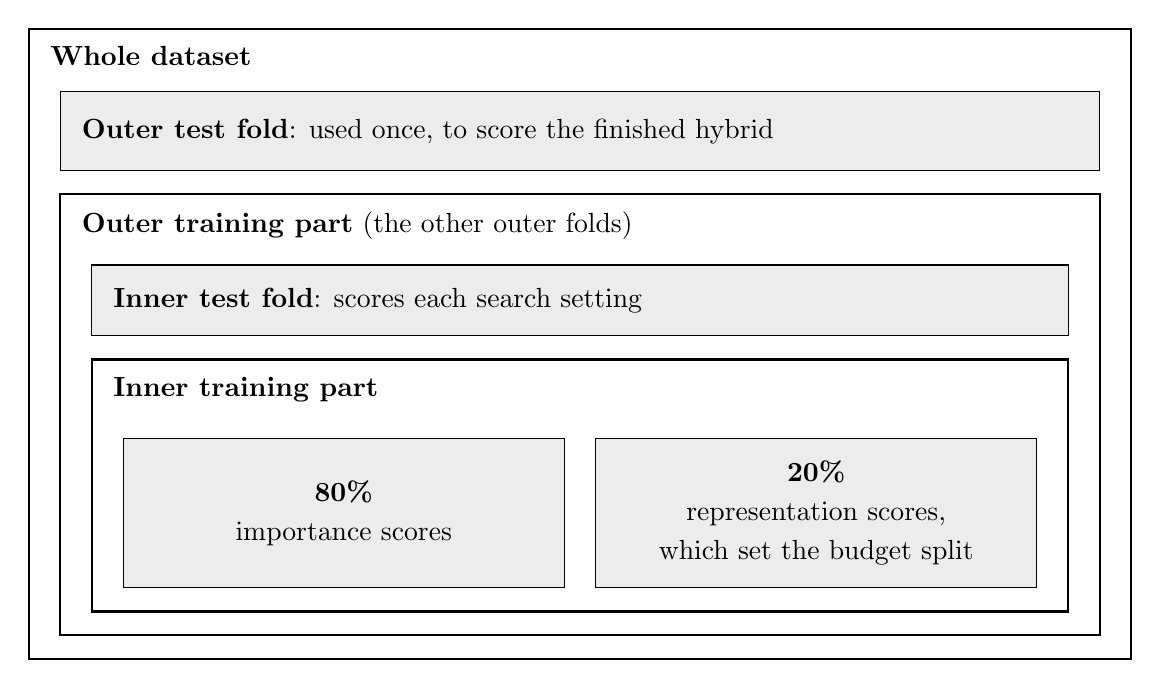
\begin{tikzpicture}[x=1cm,y=1cm]
    % whole dataset
    \draw[thick] (0,0) rectangle (14,8.0);
    \node[anchor=north west] at (0.15,7.9) {\textbf{Whole dataset}};
    \draw[fill=gray!15] (0.4,6.2) rectangle (13.6,7.2);
    \node[anchor=west] at (0.55,6.7) {\textbf{Outer test fold}: used once, to score the finished hybrid};
    % outer training part
    \draw[thick] (0.4,0.3) rectangle (13.6,5.9);
    \node[anchor=north west] at (0.55,5.8) {\textbf{Outer training part} (the other outer folds)};
    \draw[fill=gray!15] (0.8,4.1) rectangle (13.2,5.0);
    \node[anchor=west] at (0.95,4.55) {\textbf{Inner test fold}: scores each search setting};
    % inner training part
    \draw[thick] (0.8,0.6) rectangle (13.2,3.8);
    \node[anchor=north west] at (0.95,3.7) {\textbf{Inner training part}};
    \draw[fill=gray!15] (1.2,0.9) rectangle (6.8,2.8);
    \node[align=center] at (4.0,1.85) {\textbf{80\%}\\[2pt]importance scores};
    \draw[fill=gray!15] (7.2,0.9) rectangle (12.8,2.8);
    \node[align=center] at (10.0,1.85) {\textbf{20\%}\\[2pt]representation scores,\\[2pt]which set the budget split};
\end{tikzpicture}
\caption[The three levels of splitting.]{The three levels of splitting, each inside the one before. Every split keeps each group whole.}
\label{fig:split_levels}
\end{figure}

For each representation $k$, the importance method gives every feature a score $s^{(k)}_j \ge 0$, computed on the 80\% part of the internal split (Figure~\ref{fig:split_levels}). These scores rank features only within their own base representation. The standalone score $r_k$ is the score of the internal evaluator, trained on representation $k$ in the 80\% part and scored on the 20\% part, in the dataset's metric. These scores cannot be compared across metrics as they stand: a lower RMSE is better and it has no fixed upper limit, whereas a Spearman correlation is higher when better and lies between $-1$ and 1. Before the budget is split, each $r_k$ is therefore converted to a score $\tilde r_k$ on which 0 means the representation predicts no better than a trivial predictor and 1 means it predicts perfectly. The trivial predictor depends on the metric. For Spearman, Pearson, the Matthews correlation coefficient (MCC) and $R^2$, $\tilde r_k = \max(0, r_k)$. For AUROC and the concordance index, $\tilde r_k = \max(0, 2(r_k - 0.5))$. For RMSE, $\tilde r_k = \max(0, 1 - \mathrm{RMSE}_k/\mathrm{RMSE}_0)$, where $\mathrm{RMSE}_0$ is the error of predicting the training mean, and mean absolute error is rescaled likewise against the training median. For accuracy and weighted F1, $\tilde r_k = \max(0, (r_k - r_0)/(1 - r_0))$, where $r_0$ is the score of always predicting the majority training class.

An optional representation count $N$ keeps the $N$ representations with the highest standalone scores on the fold and discards the rest for that iteration of the search. Each remaining representation receives a weight $w_k = g(\tilde r_k)$, with $g$ set by the allocation method, and a share $b^*_k = B\, w_k / \sum_l w_l$ features, rounded by largest remainder and capped at its width. A representation left out by the representation count, or whose standalone fit fails, receives no features. Thus $\sum_k b_k = \min(B, \sum_k d_k)$ and $b_k \le d_k$, and a representation with $w_k > 0$ keeps at least one feature. The global pool does not use these shares (see below).

Let $S_k$ be the top $b_k$ features of representation $k$ by $s^{(k)}_j$, among those with $s^{(k)}_j > 0$; if none scores above 0, its full $b_k$ is taken. The cut exists because tree importance gives exactly 0 to every feature no tree split on, and filling the budget with those would pick them by their position in the matrix. The hybrid is $\mathbf{H} = [\mathbf{X}^{(1)}_{:,S_1}, \dots, \mathbf{X}^{(K)}_{:,S_K}]$, with $\sum_k |S_k| \le B$, so it can be narrower than its budget.

The hybrid search returns a list of settings for feature selection, referred to here as a configuration. It is scored by fitting the downstream model on the hybrid in each fold of the search and averaging the held-out scores. Each pair of downstream model and budget has its own search, and thus its own winner. Because this score is chosen over a range of selected configurations, it is optimistic \citep{Varma2006, Cawley2010}. However, so is its direct comparison with the highest-performing base representation on the dataset. The whole search runs inside each outer training fold, and the winning settings are rebuilt there and scored once on the untouched outer test fold, both for the winner at each budget and for each downstream model's best across budgets. The inner search score minus the outer test score is \textbf{[RESULT NEEDED: inner minus outer test score, per dataset, in its own metric]}.

Chapter~\ref{chap:similarity} uses two variants of this search. Under label noise, training quantities use noisy labels while held-out scoring uses clean labels unless. Under the nearest-neighbor objective, each molecule's activity is predicted from its five nearest neighbors in the feature space, as discussed in Chapter~\ref{chap:similarity}.

% TODO: Figure 5.1: the search pipeline schematic.

\paragraph{Blueprints.}

As explained above, a hybrid search returns a list of settings that function as a feature selection method to generate the hybrid representation itself. These settings are recorded in a blueprint that can be used on new folds of the same dataset or even new data. The blueprint contains additional information, including some fields for analysis, meta-data, and scores. These scores are used only for comparative purposes as in this research, the hybrids are rebuilt per-fold and are scored as such. 

Listing~\ref{lst:blueprint} lists every field of a blueprint and its type.
\begin{lstlisting}[float=htbp, breaklines=true, basicstyle=\scriptsize\ttfamily, columns=fullflexible, keepspaces=true, frame=single, caption={Fields of a blueprint and their types. Comment lines group the fields, and each field is given with its type and, where needed, a comment on its meaning.}, label=lst:blueprint, captionpos=b]
Blueprint
  # What the search chose. A rebuild reads all of these.
  reps                  : list[str]           # every representation searched, not only those used
  rep_count             : int or None         # how many of them may contribute; None = all
  budget                : int                 # most features the hybrid may have
  allocation_method     : str
  importance_method     : str
  internal_evaluator    : str
  objective             : str                 # 'predictive' or 'similarity'

  # How the search scored configurations.
  metric                : str
  lower_is_better       : bool
  task_type             : str                 # 'regression' or 'classification'
  n_folds               : int
  seed                  : int

  # Augmentation settings. A rebuild reads all of these.
  augmentation_strategy : str
  aug_per_source_budget : int, or {source: int}, or None
  augmentation_margin   : float
  augmentation_fraction : float or None
  candidate_ranking     : str
  augmentation_threshold: float or None
  augmentation_budget   : int
  aug_max_candidates    : int

  # Stored for inspection.
  rep_scores            : {representation: float}
                          # each representation's best score over every molecule the search saw;
                          # the rebuild uses it to choose which representations to keep only when
                          # rep_count is set and no per-fold scores are given
  allocation_per_fold   : {fold: {representation: int}}      # features each representation got
  kept_augmentations    : {fold: {source: list[int]}}         # extra features kept, by index
\end{lstlisting}


The blueprint does not record the specific features that are returned by the hybrid, as it is meant to be re-run using the same settings on new, labeled data. Alternatively, you can reuse the features of a labeled fit and apply them to data with no labels under the assumption that the same features matter between sets. 

The blueprint is extended by an additional explainbility layer. Since it does not store feature names, this additional step runs on a completed hybrid, records where each selected feature came from and, wherever possible, what that feature means. An ECFP4 bit is named by the atom environment that sets it, written as a SMILES fragment from a molecule with the bit set. MACCS keys are named by their SMILES arbitrary target specification (SMARTS) pattern and a short name, and descriptor features by descriptor name. Protein composition, descriptor and k-mer features, antibody composition, one-hot, BLOSUM, structural and inverse-folding features, gene-expression pathway sets and PCA components are named too. MAP4 and DRFP features get only a bit index, and Avalon, Mordred, atom-pair, graph-kernel and learned-embedding features only the representation name and dimension index.

\subsection{The search space}\label{sec:method:searchspace}
% TODO: am I keeping nanobody thermostability?? This is a question for post dataset selection (ie. now)
To run a hybrid search, we first measure feature importance, select how many features to take from each contributing base representation, and how to score a candidate feature set. And for each of those steps, there's no one right way to do it. Different prediction tasks prefer different methods of scoring feature importance or candidate features, different sets of input hybrids, and so forth. The search tries to find the ideal settings for the hybrid feature selection process, tailor to given dataset and downsream model. All combinations of settings values are explored, as the settings interact. The best budget depends on the downstream model, as shown below for nanobody thermostability. This search grid also tests the chapter's claim that no single setting suits every dataset.

Six settings in total are searched, namely the downstream model, the budget, the representation count, the importance method, the allocation method and the internal evaluator. Table~\ref{tab:search_tiers} gives default search settings, organised by runtime speed, and Table~\ref{tab:decided_grid} the smaller set searched on each dataset in this chapter (Section~\ref{sec:method:decided_grid}).  The importance methods tested are LightGBM gain, TreeSHAP or DeepLIFT (Section~\ref{sec:method:importance}). Feature-level importance depends on the model as well as on the data \citep{Dong2020}, and as such we observe that within the search, a different ranking of features produces a different hybrid output.

The downstream model is trained on the hybrid representation. This model can be a supervised model of any form, classification or regression. We used random forest, XGBoost, LightGBM, SVM, a deep neural network (DNN) and a Gaussian process. Each dataset in this chapter uses two of them (Section~\ref{sec:method:models}). 

The budget is the maximum number of features in the hybrid, taken from eight values (10, 25, 50, 100, 250, 500, 1,000 and 2,000 features). When the budget is too small, informative features can be left out, yet when it is too large it will pick up on too many uninformative ones, especially ones that give small datasets room to overfit. 

\textbf{[RESULT NEEDED: best budget per downstream model on nanobody thermostability, full runs]}

We select a set of up to 10 base representations per dataset, chosen prior to the search (Table~\ref{tab:dataset_reps}). The selections were made based on each representation's relative performance on the prediction task. We took into account what type of information each representation contained, and tried to span a wide set across the selected 10. For example, while there are many high-performing graph-based embeddings in QSAR modelling, for the purposes of testing a feature selection process which takes features from different sources of information, it is better to have a mix of graph-based embeddings, as well as other types of molecular representations like substructure fingerprints, property vectors, sequential embeddings, etc.  The representation count (2, 3, 5 or all) sets how many may contribute features, keeping those with the highest standalone scores on each fold. The number of representation counts to test is searched in the sweep as datasets differ in how many representations have features worth selecting, and pooled feature selection over all representations has no such setting. While we tested various methods of pooling the features, we found computing feature importance scores and concatenation techniques on a global pooled feature set was far less effective than when the feature scoring is kept on a per-representation basis. Since the features contain different types of information at different scales, pooling the features too early makes comparisons within in the pool challenging. We found that it's better to determine which features are important to each representation first, and go from there.

Every allocation method is paired with every count. In preliminary runs, some datasets performed best with 2 or 3 representations and others with all 10. \textbf{[RESULT NEEDED: datasets best with 2 or 3 representations and with all, full runs]}

\subsubsection{Feature importance scoring}

We score run a feature importance scoring method on each base representation which gives each features a single positive score. These scores remain relative within a given representation, so they are not compared or normalised between representations.  Split-based tree importance is biased toward features with many possible split points \citep{Strobl2007}, which matters here because we use binary fingerprint bits alongside continuous embeddings. No single importance method works best across datasets and downstream models. After testing a wider variety of methods found across literature, we settled three methods whose rankings did not correlate strongly with each other and whose selected features performed well as model input (Additional file~\ref{app:add:design_experiments}).

We score features using LightGBM gain importance, SHapley Additive exPlanations (SHAP) values for tree ensembles (TreeSHAP) and DeepLIFT (Deep Learning Important FeaTures) \citep{Shrikumar2017}. LightGBM gain measures how much a feature reduced the training loss where trees split on it \citep{ke2017lightgbm}. TreeSHAP gives each feature's exact Shapley value for each molecule's prediction from a tree model \citep{Lundberg2020}. DeepLIFT measures how much a feature moves the output of a small network, trained with Adam \citep{Kingma2015}, away from its output on an all-zero reference input, which after standardization places every feature at its training mean \citep{Shrikumar2017, Kokhlikyan2020, Ancona2018}. On Caco-2, the median share of features scoring above 0 was 30\% for LightGBM gain, 70\% for TreeSHAP and 90\% for DeepLIFT (preliminary, over 10 representations and 3 folds). Table~\ref{tab:importance_methods} gives the settings of each method, including the pre-screen of representations wider than 2,000 features.

% CODE INPUT
\begin{table}[htbp]
\centering
\small
\begin{adjustbox}{max width=\textwidth,max totalheight=0.78\textheight}
\begin{tabular}{@{}P{0.15\linewidth}P{0.24\linewidth}P{0.22\linewidth}P{0.17\linewidth}P{0.16\linewidth}@{}}
\toprule
Method & Model fitted per representation & Score of one feature & Classification labels & Representations over 2{,}000 features \\
\midrule
LightGBM gain & LightGBM, 50 trees, depth 6 & Summed loss reduction of its splits; 0 if never split on & One model on the class labels & 2{,}000 highest-variance features fitted; the rest score 0 \\
TreeSHAP & RF, 50 trees, depth 10 & Mean absolute SHAP value over training molecules & Binary: positive class; multiclass: mean over classes & As for LightGBM gain \\
DeepLIFT & NN, ReLU layers of 64 and 32 units, 100 epochs of Adam, learning rate 0.001 & Mean absolute attribution against an all-zero reference (Rescale rule) & Binary: positive class; multiclass: mean over classes & Every feature scored \\
\bottomrule
\end{tabular}
\end{adjustbox}
\caption[Settings of the importance methods.]{Settings of the importance methods, fitted per representation and fold. Unlisted settings are library defaults.}
\label{tab:importance_methods}
\end{table}


% TODO: review, needs manual review -- corrected 2026-10-08 to the per-dataset grid
Each dataset searches one, two or all three importance methods (Table~\ref{tab:decided_grid}).



\subsubsection{Feature allocation methods}\label{sec:method:allocation}
% [notes moved to thesis_notes_moved.md]


% TODO: review, needs manual review
The allocation method decides how many of the $B$ features each representation contributes; the importance method decides which. Of the five methods searched, four give each representation a fixed share computed from its rescaled standalone score (linear, squared, softmax and rank-decay allocation). The fifth, the global pool, lets the candidate features offered by every representation compete in one importance ranking.

% Old greedy allocation, cut; kept for reference:

% \begin{enumerate}
%     \item \textbf{Split:} Divide training data into allocation-train (80\%) and validation (20\%) subsets using scaffold splitting.

%     \item \textbf{Initialize:} Set current feature set to empty, remaining budget to $B$.

%     \item \textbf{Rank features:} For each representation $r \in \{base_1, base_2, \dots base_m\}$, train RFs using the base representations individually, then rank features by mean decrease in impurity.

%     \item \textbf{Iterate:} While remaining budget $\geq$ step\_size and patience not exhausted:
%     \begin{enumerate}
%         \item For each representation, try adding the top step\_size candidates from its ordered list to the current feature set.
%         \item Train a RF using the tentative feature set.
%         \item Evaluate $R^2$ on the validation set.
%         \item Select the representation whose addition yields the highest validation $R^2$.
%         \item Permanently add step\_size features from the winning representation; remove from its candidate list.
%         \item If validation $R^2$ does not improve for patience consecutive rounds, terminate early.
%     \end{enumerate}

%     \item Re-compute importance scores for the features of the new hybrid on the full training data. For each representation, select the top $n_r$ features according to the allocation determined above, where $n_r$ is the number of features allocated to representation $r$ during iteration.
% \end{enumerate}

% This greedy approach works better on larger datasets, as the size of the validation set may not be enough to gain meaningful insights from.


% TODO: review, needs manual review
The four fixed-share methods compute shares from the standalone score on the internal validation part. Only linear allocation makes the share proportional to that score. All four assume that representations with stronger predictive performance contribute more valuable features.




% TODO: review, needs manual review
The assumption fails when a strong representation owes its score to a few features, so that a large share fills with weak ones. Fixed shares also ignore complementarity, so two representations carrying the same information both receive a share. Only the global pool ranks features from different representations against each other.

% TODO: explain why the greedy approach was tried, but it's too computationally intensive and actually quite ineffective
% TODO: explain framework experiments and how they helped here

% CODE INPUT
% TODO: review, needs manual review
The fixed-share methods differ only in how $w_k$ is computed from $\tilde r_k$ (Table~\ref{tab:alloc_methods}), with settings fixed for every dataset. Under linear and squared allocation, a representation with rescaled score 0 receives 0 features. Under softmax and rank decay, no representation receives 0 features because of its score. Since every rescaled score lies between 0 and 1, softmax cannot give one representation most of the budget, and with 10 representations the best takes at most 23.2\% of it. Rank decay uses only the order, so with 10 representations the best receives 27.3\% and the tenth 1.8\%, whatever the gaps between their scores. Table~\ref{tab:alloc_example} gives a worked example.

% CODE INPUT
\begin{table}[htbp]
\centering
\small
\begin{adjustbox}{max width=\textwidth,max totalheight=0.78\textheight}
\begin{tabular}{@{}P{0.13\linewidth}P{0.24\linewidth}P{0.14\linewidth}P{0.24\linewidth}P{0.19\linewidth}@{}}
\toprule
Method & Weight $w_k$ & Fixed setting & How features are chosen & When a representation receives 0 features \\
\midrule
Linear & $\tilde r_k$ & none & Top $b_k$ of its own ranking & $\tilde r_k = 0$ \\
Squared & $\tilde r_k^{\,2}$ & power 2 & Top $b_k$ of its own ranking & $\tilde r_k = 0$ \\
Softmax & $\exp\big((\tilde r_k - \max_l \tilde r_l)/T\big)$ & $T = 1$ & Top $b_k$ of its own ranking & never from its score \\
Rank decay & $e^{-0.3\rho_k}$, $\rho_k$ = rank by score, 0 for the best & decay 0.3 & Top $b_k$ of its own ranking & never from its score \\
Global pool & $\tilde r_k^{\,2}$, sizing its offer to a pool of $2B$ candidates & power 2; pool $2B$ & Top $B$ of one joint ranking over all offered candidates & $\tilde r_k = 0$, or none of its candidates in the joint top $B$ \\
\bottomrule
\end{tabular}
\end{adjustbox}
\caption[The five allocation methods searched.]{The five allocation methods. $w_k$ is the weight computed from representation $k$'s rescaled standalone score $\tilde r_k$, $B$ is the budget, $b_k$ is the share of representation $k$, $\rho_k$ is its rank by score and $T$ is the softmax temperature.}
\label{tab:alloc_methods}
\end{table}

% CODE INPUT
\begin{table}[htbp]
\centering
\begin{adjustbox}{max width=\textwidth,max totalheight=0.78\textheight}
\begin{tabular}{@{}lccc@{}}
\toprule
Method & $\tilde r_1 = 0.6$ & $\tilde r_2 = 0.5$ & $\tilde r_3 = 0.2$ \\
\midrule
Linear & 46 & 39 & 15 \\
Squared & 55 & 39 & 6 \\
Softmax & 39 & 35 & 26 \\
Rank decay & 44 & 32 & 24 \\
\bottomrule
\end{tabular}
\end{adjustbox}
\caption[Worked example of the four fixed-share allocation methods.]{Worked example of the four fixed-share allocation methods for a budget of 100 features and three representations. Each entry is the number of features a representation receives, with shares rounded by largest remainder.}
\label{tab:alloc_example}
\end{table}

% CODE INPUT
% TODO: review, needs manual review
The global pool sizes each representation's offer with squared weights $\tilde r_k^{\,2}$, as shares of a pool of $2B$ candidate features, each offer capped at the representation's width and holding only features scoring above 0. The same importance method is fitted once on the joined offers, and the hybrid keeps the top $B$ features that score above 0. Each representation's count is therefore an outcome of the joint ranking, with no minimum of one feature, and a feature's rank depends on what the other representations offered. The cost is one extra importance fit per configuration.


% CODE INPUT
% TODO: review, needs manual review
The five methods were chosen in a preliminary comparison (Additional file~\ref{app:add:design_experiments}).

\subsubsection{Search configuration and internal evaluation}

The most useful features for an RF may not be the most useful for an SVM, and vice versa. The relative importance of a feature is dependent on the model \citep{Dong2020}. Within the search grid, we us an internal evaluator to fit on one candidate feature set at a time. This process is separate from the final downstream model evaluation. In a standard search, four internal evaluators are used: RF, DNN, LightGBM, and the matched evaluator. When the internal evaluator is set to \texttt{match}, the search scores each candidate hybrid on the same model type as the downstream model, for each of the twelve model types used in this thesis. This means that internal evaluators outside the standard sweep may be tested.  For a downstream model outside of the pre-defined set, if no matched evaluator exists in the code, and the search uses the other internal evaluators that were requested. Each internal evaluator is fitted on the internal training fold and scores on the internal validation fold within that CV iteration using the dataset's specified evaluation metric. 

% CODE INPUT
% TODO: review, needs manual review -- moved up from the end of this subsection and reworded to follow your paragraph above
A random forest, LightGBM or DNN downstream model is searched with three internal evaluators, because its matched evaluator is already one of the other three. An XGBoost, SVM or Gaussian process downstream model is searched with four, because the matched evaluator adds one of its own family. Only the DNN evaluator shares its downstream model's architecture and training settings, and even it draws its 20\% early-stopping molecules at random, whereas the downstream DNN splits them by the outer split's groups. Additional file~\ref{app:add:model_settings} gives every evaluator setting.

The internal evaluator's scores determine how the budget is split and which representations are kept. The internal evaluator ranks candidate feature sets, it does explicity not rank features within a representation. This process of selecting a feature set by fitting a model on it, and keeping the set that scores the best is known as the wrapper method \citep{Kohavi1997}. This is distinct from a filter method which scores features without fitting a model. 

% TODO: review, needs manual review -- added sentence pointing to where the scores are used
Section~\ref{sec:method:allocation} gives how each allocation method turns these scores into a number of features per representation.


% TODO: review, needs manual review -- corrected 2026-10-08: the old counts (8,160, 10,080, 816) were for the full default grid. The per-dataset counts in Table tab:decided_grid were computed with the engine's counting rule (src/kirby/find_best_hybrid.py:612-634), not read from a run log. Additional file app:add:search_size still gives the old breakdown and needs the same update.
The search tests every combination of the six settings on a dataset under 5-fold cross-validation. Over every value of Table~\ref{tab:search_tiers}, this is 8,160 configurations with five downstream models; with each dataset's own values it is 63 to 3,360 (Table~\ref{tab:decided_grid}).

% TODO: review, needs manual review -- written for your TODO "mention representation knobs", read as the representation count. Values checked against DEFAULT_REP_COUNTS in src/kirby/find_best_hybrid.py:3105.
Of the six settings, the representation count is the only one that acts on whole representations. At each count (2, 3, 5 or all), only the representations with the highest internal evaluator scores on that fold contribute features, so the internal evaluator decides which representations are kept as well as how the budget is split among them (Section~\ref{sec:method:searchspace}).


% TODO: review, needs manual review
Importance scores are computed once per search fold and importance method, and each representation's internal evaluator score once per search fold and internal evaluator. Every configuration reuses them, so the cost grows more slowly than the number of configurations.

% Your original paragraph, rewritten above:
% When I began to implement this idea, I figured that there would be a fairly straightforward way to select the most informative features. However, I began to ask some questions. How do you measure feature importance? If you're starting with a handful of input representations, how many features do you take from each? How do you score these potential feature sets?  Unfortunately, my one-size-fits-all hypothesis rang true on multiple fronts. As I found out, different prediction tasks prefer different answers to all of those questions. So to figure out how to even go about selecting the best features, I realized I had to sweep a search space.

% TODO: review, needs manual review -- written for your TODO "explain framework experiments". Rule and numbers copied from the Additional file paragraph "Values of the search settings" (additional_files_body.tex), which is itself marked for manual review; not re-read from result files.
Before the full runs, we ran preliminary design experiments on 1 to 9 datasets to choose the values each setting may take. A value was kept if it gave the best score for some dataset, downstream model and budget. A setting was fixed at one value when the spread between its values was smaller than the spread of one value across folds. For example, on hERG $K_i$ with linear allocation at 300 features, five ways of rescaling each representation's score gave RMSE values from 0.5870 to 0.5924 (p$K_i$), while a single rescaling ranged from 0.5475 to 0.6294 across 5 folds, so the rescaling is one fixed rule per metric.

% TODO: review, needs manual review
Preliminary design experiments set the values each setting may take (Additional file~\ref{app:add:design_experiments}).





\subsection{Augmentation}\label{sec:method:augmentation}
% [notes moved to thesis_notes_moved.md]


% TODO: review, needs manual review
Some feature sets are too small or too specialized to take part in budget allocation, such as MACCS fingerprints (167 features) or log-likelihood ratios (3 features). Others, such as mutation features that record differences from a parent antibody, carry meaning only beside a full representation. Excluding them would lose potentially useful signal, but including them would distort the budget split, since they cannot contribute many features. We therefore add them as augmentation, calling the finished hybrid $\mathbf{H}$ the base and the feature sets that supply extra features the donors.

% TODO: I need a better list to describe augmentations

% TODO: review, needs manual review
Donors are set per dataset (Augmentation column of Table~\ref{tab:dataset_reps}). They range from small fingerprints such as MACCS to structural sets such as 3D pharmacophores and Coulomb matrix eigenvalues, and include features that describe only differences between variants, such as antibody mutation features. MACCS is a donor on four of the six small-molecule datasets and a base representation on MDR1--MDCK efflux. On QM9, MACCS is not offered and the topological torsion fingerprint (2,048 features) is a donor, the only wide one. \citet{Bahia2023} found that combining 2D and 3D descriptors gave many more significant models across six protein--ligand series (461 structures), which they attribute to complementary properties. Their 3D descriptors came from bioactive conformations in the Protein Data Bank, whereas our 3D donors use one generated conformer per molecule.

% CODE INPUT
% TODO: review, needs manual review
Donor features are ranked by what the base gets wrong. Inside each outer training fold, an 80/20 internal split keeps each scaffold or sequence group on one side. A small random forest (50 trees, depth at most 10) is fitted on the base features, and 3-fold group-aware cross-validation gives out-of-fold residuals $r_i = y_i - \hat{y}^{\mathrm{oof}}_i$ for the internal-training molecules, where for binary tasks $\hat{y}$ is the positive-class probability. In-sample residuals would shrink toward zero. All donor features are pooled, each is scored by its absolute Pearson correlation with the residuals, $c_j = |\rho_{\mathrm{P}}(\mathbf{x}_j, \mathbf{r})|$, and the top $M = 50$ go forward. Ranking against $\mathbf{y}$ would favor features that repeat what the base captures; ranking against $\mathbf{r}$ favors features that explain its errors, as in gradient boosting \citep{friedman2001greedy} and least angle regression \citep{efron2004lars}.

% CODE INPUT
% TODO: review, needs manual review
Blocks of the top $k \in \{0, 5, 10, 20, 40\}$ ranked features, capped at the number of candidates, are each added to the base and scored with the downstream model on the internal-validation molecules. The chosen $k^*$ has the best score and must beat $k=0$, which wins ties, so keeping no extras is the default. Five block choices instead of about 50 accept-or-reject decisions leave less room to overfit a small validation set \citep{Cawley2010}. The chosen donors and feature positions are stored and re-extracted for the outer fold.

% CODE INPUT
% TODO: review, needs manual review
In uncapped mode, extras are appended outside the budget, so the final width is $|\mathbf{H}| + k^*$, at most $B + 40$ features. In capped mode, they displace base features and the width stays at most $B$. The base features are ranked once by random forest importance (50 trees, depth at most 10) and the $k^*$ weakest are dropped, after any unspent budget is filled, keeping at least one base feature. Uncapped augmentation and no augmentation differ in width at the same $B$, so their comparison mixes better features with more features. Capped mode, where an extra must beat a base feature, removes this difference.

% CODE INPUT
% TODO: review, needs manual review
% TODO: review, needs manual review -- corrected 2026-10-08: augmentation is cut on all 16 datasets (DECISIONS.md Step 8; enforced in tests/experiments/_shared.py). The decoy test and the Koenig sentence were removed because neither runs on the 16 datasets (c21 runs its extra-feature arms only on ginkgo_colloidal and ginkgo_hic).
Augmentation is a separate condition rather than a searched setting, so a dataset with donors is searched three times, with no, uncapped and capped augmentation. In an earlier search of each whole dataset, 14 of the 16 datasets ran all three, while humanness and trastuzumab--HER2 binding have no donors. On none of the 16 did either augmented condition score better than no augmentation by more than 1\% (3\% on datasets under about 1,000 samples), so the searches in this chapter run without augmentation (Section~\ref{sec:method:decided_grid}). In a second use, a user keeps one strong representation at full width as the base and adds a few extras, with $B$ its width, so only uncapped mode makes sense. This use matters for adoption, because a chemist can keep the representation they already trust and learn which few outside features help, and how many. Augmentation also asks directly whether another representation holds signal the base lacks (Chapter~\ref{chap:flaws}).

% CODE INPUT
% TODO: review, needs manual review
The residual ranking has four limitations. $|\rho_{\mathrm{P}}|$ captures only linear relations, one feature at a time. It ignores redundancy, so two near-identical donor features can both rank high. Donors are pooled with no per-donor limit, so a 2,048-feature donor gets more chances than a 49-feature one. Finally, the margin over $k=0$ is zero, so a near-tie on one internal split can admit extras.

% CODE INPUT
% TODO: review, needs manual review
Table~\ref{tab:aug_conditions} summarizes the three conditions.

% CODE INPUT
\begin{table}[htbp]
\centering
\small
\begin{adjustbox}{max width=\textwidth,max totalheight=0.78\textheight}
\begin{tabular}{@{}P{2.4cm}P{3.0cm}P{4.6cm}P{3.6cm}@{}}
\toprule
Condition & Final width (features) & What an extra feature must beat & Datasets that run it \\
\midrule
No augmentation & at most $B$ & nothing is offered & all 16 \\
Uncapped & $|\mathbf{H}| + k^*$, at most $B + 40$ & keeping no extras & none (cut after the earlier search) \\
Capped & at most $B$ & keeping no extras, and the weakest base feature it replaces & none (cut after the earlier search) \\
\bottomrule
\end{tabular}
\end{adjustbox}
\caption[The three augmentation conditions.]{The three augmentation conditions. $B$ is the budget and $|\mathbf{H}|$ the width of the base hybrid, both in features, and $k^*$ is the chosen number of extra features, which are drawn from a small or specialized feature set offered to the hybrid.}
\label{tab:aug_conditions}
\end{table}


\subsection{Search grid per dataset}\label{sec:method:decided_grid}
% TODO: review, needs manual review -- new 2026-10-08, replaces "Fast Tier and Adaptive Pruning" and "Search Tier Settings". Source: scratchpad/precompute_cuts/DECISIONS.md (your decisions of 2026-10-03, seven budget rows and six importance rows revised by hand that day, suzuki 2026-10-07) as applied by tests/experiments/decided_grid.json. The budget rule below is the Step 2 (v3) rule; the rules for the other settings (Steps 3-6) are summarized as "clearly worse", so check whether you want them stated exactly.
Searching every value of Table~\ref{tab:search_tiers} in every fold of every dataset was too slow, so each dataset searches a smaller grid (Table~\ref{tab:decided_grid}). The grid was chosen from an earlier search of each whole dataset. On each dataset we kept the two downstream models with the best scores, and the budgets whose ten best configurations scored within 1\% of the best budget (3\% on datasets under about 1,000 samples), widened to at least three consecutive budgets. Importance methods, allocation methods, internal evaluators and representation counts that scored clearly worse than the best were dropped.
% TODO: review, needs manual review -- where the grid came from: the earlier whole-dataset search scored configurations on folds that held each dataset's later test samples, so the choice of grid saw those samples (HANDOFF_PER_FOLD_ALIGNMENT.md §3 says the thesis must state this). The grid is the only thing it chose: every search reported in this chapter runs inside one outer fold, on that fold's training samples only.

% TODO: review, needs manual review
Four datasets, QM9, trastuzumab--HER2 binding, H3K4me3 and TATA promoter, were too slow for the earlier search over every value. They were searched over a shorter fixed list, called the fast tier (LightGBM gain importance; linear, squared and rank-decay allocation; three or all representations), and their grid stays within it. The search with the nearest-neighbor objective has its own grid, given in Chapter~\ref{chap:similarity}.

% TODO: review, needs manual review -- table rewritten 2026-10-08: the method's full list of values; the fast-tier column moved into the text and Table tab:decided_grid
\begin{table}[htbp]
\centering
\begin{adjustbox}{max width=\textwidth,max totalheight=0.78\textheight}
\begin{tabular}{@{}P{0.30\linewidth}P{0.62\linewidth}@{}}
\toprule
Setting & Values \\
\midrule
Downstream models & Random forest, XGBoost, LightGBM, SVM$^{a}$, DNN, Gaussian process$^{b}$ \\
Internal evaluators & Matched evaluator, random forest, LightGBM, DNN \\
Feature budgets (features) & 10, 25, 50, 100, 250, 500, 1{,}000, 2{,}000 \\
Allocation methods & Linear, squared, softmax, rank decay, global pool \\
Importance methods & LightGBM gain, DeepLIFT, TreeSHAP \\
Representation counts & 2, 3, 5, all representations \\
\bottomrule
\end{tabular}
\end{adjustbox}

\smallskip
{\footnotesize $^{a}$Not fitted above 10{,}000 molecules (5{,}000 when augmentation features are added outside the budget). $^{b}$Not fitted above 1{,}000 molecules.}
\caption[Values the hybrid search can take for each setting.]{Values the hybrid search can take for each setting. The matched evaluator belongs to the same model family as the downstream model.}
\label{tab:search_tiers}
\end{table}

% TODO: review, needs manual review -- configurations per fold computed 2026-10-08 with the engine's counting rule (src/kirby/find_best_hybrid.py:612-634), not read from a run
\begin{table}[htbp]
\centering
\small
\setlength{\tabcolsep}{3pt}
\begin{adjustbox}{max width=\textwidth,max totalheight=0.78\textheight}
\begin{tabular}{@{}lllllll@{}}
\toprule
Dataset & Downstream models & Budgets (features) & Importance & Allocation & Representation counts & Configurations \\
\midrule
hERG $K_i$ & SVM, DNN & 250--2{,}000 & G, T & L, Q, S, R & all & 224 \\
LogD & DNN, SVM & 500--2{,}000 & G & L, Q, R & all & 63 \\
Caco-2 efflux & DNN, SVM & 500--2{,}000 & G, T, D & L, Q, S, R & all & 252 \\
Rat liver microsome clearance & SVM, DNN & 500--2{,}000 & G, T, D & all five & all & 315 \\
MDR1--MDCK efflux & SVM, DNN & 500--2{,}000 & G, T, D & all five & all & 315 \\
QM9$^{\dagger}$ & DNN, LightGBM & 500--2{,}000 & G & L, Q, R & 3, all & 108 \\
Buchwald--Hartwig yield$^{a}$ & Random forest, LightGBM & 500--2{,}000 & T, D & all five & 2 & 120 \\
Buchwald--Hartwig plates & Random forest, LightGBM & 100--500 & G, D & all five & 2, 3 & 360 \\
Koenig expression & SVM, DNN & 250--2{,}000 & G, T, D & all five & all & 420 \\
Nanobody thermostability & DNN, SVM & 50--2{,}000 & G, T & all five & 3, 5, all & 1{,}260 \\
Humanness & XGBoost, random forest & 10--2{,}000 & G, T, D & all five & 2, 3, 5, all & 3{,}360 \\
Trastuzumab--HER2 binding$^{\dagger}$ & XGBoost, LightGBM & 100--500 & G & L, Q, R & 3, all & 126 \\
H3K4me3$^{\dagger}$ & DNN, LightGBM & 250--2{,}000 & G & L, Q, R & 3, all & 144 \\
TATA promoter$^{\dagger}$ & LightGBM, SVM & 500--2{,}000 & G & L, Q, R & all & 63 \\
Lung adenocarcinoma vs squamous & LightGBM, XGBoost & 10--2{,}000 & G, T, D & all five & 2, 3, 5, all & 3{,}360 \\
Breast cancer PAM50 subtype & DNN, SVM & 25--2{,}000 & G, T, D & all five & 3, 5, all & 2{,}205 \\
\bottomrule
\end{tabular}
\end{adjustbox}

\smallskip
{\footnotesize $^{\dagger}$Fast tier. $^{a}$Internal evaluators are the matched evaluator, random forest and LightGBM; every other dataset uses all four of Table~\ref{tab:search_tiers}.}
\caption[Search grid of each dataset.]{Search grid of each dataset. One row is one dataset. Budgets are consecutive values of Table~\ref{tab:search_tiers}. Importance: G, LightGBM gain; T, TreeSHAP; D, DeepLIFT. Allocation: L, linear; Q, squared; S, softmax; R, rank decay; all five adds the global pool. Configurations is the number scored in one search, over both downstream models.}
\label{tab:decided_grid}
\end{table}

% TODO: review, needs manual review -- new 2026-10-08. Numbers from /Volumes/seagate/slim_precompute/herg_ki.slim.db (the stored whole-dataset search the cuts were decided from), tier general, augmentation none, 8,220 configurations; cuts applied in the order of DECISIONS.md. Fitting time is the time_seconds stored per configuration, summed; shared importance and standalone fits may not be included in it.
Table~\ref{tab:cut_walkthrough} follows one dataset, hERG $K_i$, through the cuts. Its earlier search scored 8,220 configurations without augmentation, over six downstream models including kNN. The best had an RMSE of 0.5472 p$K_i$ (SVM, 1,000 features, LightGBM gain, softmax allocation, random forest evaluator, all representations), with a standard deviation over the five folds of 0.0443 p$K_i$. Keeping only the SVM and the DNN removed 71\% of the recorded fitting time, mostly XGBoost (35\%) and LightGBM (25\%), whose best configurations scored 0.5842 and 0.5707 p$K_i$. The budget, importance, allocation and representation-count cuts then removed most of the rest. The best configuration removed by each of these four cuts was 0.0051 to 0.0154 p$K_i$ behind the best kept, less than the spread over folds. The final grid keeps 224 configurations and 1.4\% of the fitting time, and still contains the best configuration. The cuts were chosen on this same search, so keeping its best configuration is expected; the walk-through shows how much each cut removes and how close the best removed configuration came.

% TODO: review, needs manual review
\begin{table}[htbp]
\centering
\small
\begin{adjustbox}{max width=\textwidth,max totalheight=0.78\textheight}
\begin{tabular}{@{}lcccc@{}}
\toprule
Step & Configurations kept & Fitting time kept (\%) & Best kept & Best removed \\
\midrule
Full search & 8{,}220 & 100.0 & 0.5472 & -- \\
Downstream models: SVM and DNN only & 3{,}360 & 28.7 & 0.5472 & 0.5707 \\
Budgets: 250 to 2{,}000 features & 1{,}680 & 20.0 & 0.5472 & 0.5626 \\
Importance: DeepLIFT removed & 1{,}120 & 16.3 & 0.5472 & 0.5523 \\
Allocation: global pool removed & 896 & 4.6 & 0.5472 & 0.5536 \\
Representation count: all only & 224 & 1.4 & 0.5472 & 0.5545 \\
\bottomrule
\end{tabular}
\end{adjustbox}
\caption[What each cut removes from the hERG $K_i$ search.]{The hERG $K_i$ search after each cut, applied in turn. One row is one cut. Fitting time is the share of the full search's recorded fitting time that remains. Best kept and best removed are the lowest mean RMSE over five folds, in p$K_i$ (lower is better), among the configurations kept and among those the cut removed.}
\label{tab:cut_walkthrough}
\end{table}

\subsubsection{Adaptive pruning}\label{sec:method:pruning}
% TODO: review, needs manual review -- rewritten 2026-10-08 as a short subsection; the long version with Table tab:pruning_rules is in thesis.tex.bak_before_ch5_review_2026-10-08. Rules from the stored schedule in src/kirby/find_best_hybrid.py:3824-3925; the 79 and 44 hours and the "never removed the best" calibration come from the old text, not re-checked.
The search also has an adaptive pruning option, which we did not use in this research: because of time constraints, the per-dataset cuts above, which remove far more configurations, were used instead. Pruning scores every configuration on the first two of the five folds and stops scoring those that are clearly behind. Budgets are scored from smallest to largest, and once every budget up to 100 features is scored, pairs of allocation and importance method with no configuration in the better half of their group are not searched at larger budgets. Each remaining setting is then voted on within groups of configurations that share every other setting, and a value is removed if it is among the best in too few groups. The survivors are scored on the other three folds, and the best is picked as without pruning. Unlike the cuts above, pruning decides from the dataset's own fold scores during the search, so it needs no earlier search. Its cut-offs were set on five datasets so that it never removed the best configuration, and it cut the estimated run time on LogD from 79 to 44 hours. Successive halving \citep{Jamieson2016} and Hyperband \citep{Li2018Hyperband} likewise drop configurations after partial evaluations.

\section{Methods: experimental setup}
% [notes moved to thesis_notes_moved.md]
% CODE INPUT

% TODO: review, needs manual review
% CODE INPUT
Every experiment splits each dataset into outer folds as set out in Section~\ref{sec:method:datasets}, except one preliminary analysis of Koenig expression, which uses three outer folds of unequal size. The search sees only the training samples of each outer fold, and the selected features are rebuilt on them and applied unchanged to the held-out samples. Four of the experiments below (budget overfitting, the internal evaluator, the learning curves and robustness to label noise) run only the first three outer folds, except on hERG $K_i$ and trastuzumab--HER2 binding, where their searches are fast enough to run all five. % TODO: review, needs manual review -- added 2026-10-08 from tests/experiments/_shared.py OUTER_FOLDS_RUN and ALL_FOLDS_DATASETS (c05, c10, c23, c33 among the experiments this chapter describes)

% CODE INPUT
% TODO: review, needs manual review
The hybrid is compared with the best single base representation at its full number of features, which is what a user would otherwise run. This comparator is chosen per downstream model and per fold from the search's scores on the outer training samples, then refit on those samples and scored on the same held-out samples as the hybrid, so it can differ between folds. Choosing it on the held-out samples would give it an advantage that the hybrid does not get. The hybrid is held to its budget, plus any augmentation features, so the comparator is often many times wider, and both widths are recorded for every fold, since a difference between the two scores is partly a difference in width as well as in method. The main quantity per fold is the hybrid's score minus that of the best single representation, signed so that a positive value means the hybrid scored better (for RMSE the sign is flipped). Unless stated otherwise, an experiment takes from each fold's search, for each of the dataset's two downstream models, the two best single representations and the two best hybrids. % TODO: review, needs manual review -- added 2026-10-08: the "2 best base representations and 2 best hybrids per model, per fold" rule of HANDOFF_PER_FOLD_ALIGNMENT.md, as used by c10, c11, c17, c19 and the OPIG scripts

% CODE INPUT
Chapter~\ref{chap:similarity} reuses this protocol with noise added to the training labels of each outer fold, while the held-out labels stay clean.


\subsection{Datasets and splitting}\label{sec:method:datasets}
% [notes moved to thesis_notes_moved.md]

% TODO: review, needs manual review
The hybrid experiments use 16 datasets from six domains (Table~\ref{tab:datasets}), whose curation is given in Additional file~\ref{app:datasets} and whose representations are listed in Table~\ref{tab:dataset_reps}. Folds keep each group whole, with groups chosen to match what an unseen sample means in each field.



\begin{table}[htbp]
\centering
\footnotesize
\setlength{\tabcolsep}{3pt}
\begin{adjustbox}{max width=\textwidth,max totalheight=0.78\textheight}
\begin{tabular}{P{2.6cm}P{2.5cm}P{2.0cm}P{1.0cm}P{2.4cm}P{2.4cm}}
\toprule
Dataset & Label (unit) & Task, metric & $n$ & Folds grouped by (groups) & Best single representation (score) \\
\midrule
\multicolumn{6}{l}{\textit{Small molecules: ADME and toxicity}} \\
hERG $K_i$ \citep{Zdrazil2023} & p$K_i$ & regression, RMSE $\downarrow$ & 1,412 & scaffold (769) & \textbf{[RESULT NEEDED: name, score]} \\
LogD \citep{openadmet} & LogD (log units) & regression, RMSE $\downarrow$ & 5,028 & scaffold (2,413) & \textbf{[RESULT NEEDED: name, score]} \\
Caco-2 efflux \citep{openadmet} & log$_{10}$ efflux ratio & regression, RMSE $\downarrow$ & 2,158 & scaffold (1,086) & \textbf{[RESULT NEEDED: name, score]} \\
Rat liver microsome clearance \citep{fang2023, polaris} & log$_{10}$ CL$_\text{int}$ (mL/min/kg) & regression, RMSE $\downarrow$ & 3,053 & scaffold (2,625) & \textbf{[RESULT NEEDED: name, score]} \\
MDR1--MDCK efflux \citep{fang2023, polaris} & log$_{10}$ efflux ratio & regression, RMSE $\downarrow$ & 2,641 & scaffold (2,318) & \textbf{[RESULT NEEDED: name, score]} \\
\midrule
\multicolumn{6}{l}{\textit{Quantum chemistry}} \\
QM9 \citep{Ramakrishnan2014, qm9_dataset} & HOMO--LUMO gap (eV) & regression, RMSE $\downarrow$ & 9,978 & scaffold (3,452) & \textbf{[RESULT NEEDED: name, score]} \\
\midrule
\multicolumn{6}{l}{\textit{Chemical reactions}} \\
Buchwald--Hartwig yield \citep{Ahneman2018} & yield (\%) & regression, RMSE $\downarrow$ & 3,955 & additive (22) & \textbf{[RESULT NEEDED: name, score]} \\
Buchwald--Hartwig plates \citep{Ahneman2018} & yield (\%) & regression, RMSE $\downarrow$ & 4,312 & additive (24) & \textbf{[RESULT NEEDED: name, score]} \\
\midrule
\multicolumn{6}{l}{\textit{Antibodies}} \\
Koenig expression \citep{Koenig2017, Chungyoun2024} & expression enrichment ratio (no unit) & regression, Spearman $\uparrow$ & 4,275 & mutated position (225) & \textbf{[RESULT NEEDED: name, score]} \\
Nanobody thermostability \citep{ValdesTresanco2023, Chungyoun2024} & melting temperature ($^\circ$C) & regression, Spearman $\uparrow$ & 672 & 95\% identity cluster (309) & \textbf{[RESULT NEEDED: name, score]} \\
Humanness \citep{Prihoda2022} & human or not (198 : 366) & binary, AUROC $\uparrow$ & 564 & 95\% identity cluster (461) & \textbf{[RESULT NEEDED: name, score]} \\
Trastuzumab--HER2 binding \citep{Chinery2024} & binder or not (1,639 : 3,361) & binary, AUROC $\uparrow$ & 5,000 & mutations from wild type (10) & \textbf{[RESULT NEEDED: name, score]} \\
\midrule
\multicolumn{6}{l}{\textit{Nucleotide sequences}} \\
H3K4me3 \citep{DallaTorre2025} & mark present or not (9,122 : 9,122) & binary, MCC $\uparrow$ & 18,244 & chromosome (23) & \textbf{[RESULT NEEDED: name, score]} \\
TATA promoter \citep{DallaTorre2025} & promoter or not (2,637 : 2,637) & binary, MCC $\uparrow$ & 5,274 & chromosome (23) & \textbf{[RESULT NEEDED: name, score]} \\
\midrule
\multicolumn{6}{l}{\textit{Cancer genomics (TCGA)}} \\
Lung adenocarcinoma vs squamous \citep{TCGA2014LUAD, TCGA2012LUSC, Goldman2020} & tumor type (515 : 502) & binary, AUROC $\uparrow$ & 1,017 & tissue source site (68) & \textbf{[RESULT NEEDED: name, score]} \\
Breast cancer PAM50 subtype \citep{TCGA2012BRCA, Parker2009, Goldman2020} & subtype (421 : 192 : 141 : 67) & 4 classes, weighted F1 $\uparrow$ & 821 & tissue source site (19) & \textbf{[RESULT NEEDED: name, score]} \\
\bottomrule
\end{tabular}
\end{adjustbox}
\caption[Datasets and their best single representations.]{The 16 datasets of the hybrid experiments after curation, grouped by domain, with the best single base representation of each and its mean score over the five outer folds. $n$ is the number of samples, and the fold groups are given with the number of groups in parentheses. For classification tasks, the class counts are in parentheses in the label column. CL$_\text{int}$ is the intrinsic clearance, and arrows show whether lower or higher is better.}
\label{tab:datasets}
\end{table}

% TODO: review, needs manual review
\paragraph{Pre-processing.} Additional file~\ref{app:datasets} gives the shared and per-dataset pre-processing steps, with the counts after each step. The LogD and Caco-2 labels are clipped at their 1st and 99th percentiles, so on Caco-2, for example, 22 molecules share the highest label and 23 the lowest.
% TODO: review, needs manual review -- corrected 2026-10-08 against tests/find_best_hybrid_molecular.py:244-247 (on by default) and RESULT_CAVEATS.md; counts from scratchpad/thesis_code_todo/meta_caco2.npz. LogD: 62 at the top value, 54 at the bottom


% TODO: review, needs manual review -- Chapter 3 has no classification task, so stratification is no longer attributed to it.
\paragraph{Splitting rules.} As in Chapter~\ref{chap:robustness} (Section~\ref{sec:robustness:methods}), no group is split between folds. Classification folds are also stratified with a fixed seed. Every dataset uses five outer folds. No split is random, because random splitting inflates performance estimates for molecular data by placing structurally similar compounds on both sides of the train/test boundary \citep{Yang2019, Wallach2018}. On a given dataset, every representation, model and hybrid is scored on the same folds.

% TODO: review, needs manual review -- pointer now to Additional file app:datasets:ch3 (the Chapter 3 dataset differences)
\paragraph{Groups by domain.} The small-molecule and QM9 datasets are grouped by Bemis--Murcko scaffold (Section~\ref{sec:robustness:methods}), here keeping stereochemistry. On QM9 the largest group is the empty scaffold of acyclic molecules, with 1,041 of the 9,978 molecules. The two datasets from Biogen \citep{fang2023} (rat liver microsome clearance and MDR1--MDCK efflux) have 1.2 and 1.1 molecules per scaffold, respectively, so holding out a scaffold there is close to holding out single molecules. Chapter~\ref{chap:robustness} used a different scaffold key and different curation for its versions of LogD, Caco-2, hERG $K_i$ and QM9, and Additional file~\ref{app:datasets:ch3} lists the differences.

% TODO: review, needs manual review
The reaction datasets are Buchwald--Hartwig C--N couplings from high-throughput plates. Following \citet{Ahneman2018}, they are grouped by additive, so each held-out fold holds four or five additives unseen in training. The two sets share 3,955 reactions (Additional file~\ref{app:datasets}).

% TODO: review, needs manual review
In the Koenig deep mutational scan of the anti-vascular endothelial growth factor (VEGF) antibody G6, each variant carries one mutation. % TODO: review, needs manual review -- corrected 2026-10-08 against tests/antibody_baseline_survey.py:66-71 and :390-406: one group per mutated position since 2026-10-05 (modulo 5 gave exactly five groups for five folds, so splits inside a fold failed). 225 groups is from the code comment (225 positions x 19 variants = 4,275), not counted
% [CLAUDE 2026-10-09] citation fix: Kenlay2024 clusters at 95% identity (Linclust/MMseqs2) to split pretraining data; it names no linkage and does not group labelled sets.
Variants are grouped by their mutated position, giving 225 groups, so all mutations at one position fall on the same side of a split and a model cannot look up a per-position effect at test time \citep{Vieira2026}. The nanobody and humanness sets are grouped by single-linkage clusters at 95\% sequence identity, the identity threshold \citet{Kenlay2024} used to cluster their pretraining sequences. The trastuzumab variants differ from the wild type only in the ten residues of CDR-H3 and are grouped by how many of them are mutated.

% TODO: review, needs manual review
The two nucleotide tasks, from the revised Nucleotide Transformer benchmark \citep{DallaTorre2025}, are grouped by chromosome, so each held-out fold holds two to six of the 23 chromosome groups (Additional file~\ref{app:datasets}).

% TODO: review, needs manual review
The TCGA datasets use RNA sequencing (RNA-seq) expression and other measurements of primary tumors, one per patient, from UCSC Xena \citep{Goldman2020}. Samples are grouped by tissue source site, the institution that supplied the sample, so a model cannot score well by recognizing the site.

% TODO: review, needs manual review
\paragraph{Consequences of the grouping.} Some groupings give very unequal folds. The trastuzumab held-out folds range from 13 to 3,035 variants, with binder shares from 15.5\% to 92.3\% against 32.8\% overall, and the breast cancer folds from 3 to 403 tumors. None of the 68 lung sites supplied both tumor types, so one lung fold holds 20 adenocarcinomas and 113 squamous tumors. Per-fold scores on these datasets spread more widely, so results are read per dataset and never pooled.
\subsection{Representations by domain}\label{sec:method:reps}
% [notes moved to thesis_notes_moved.md]
% TODO: review, needs manual review

Any representation that gives one fixed-length vector per sample can serve as a base representation (Section~\ref{sec:method:build}). The first version of the method used three molecular representations: PDV, ECFP4 and MHG-GNN. These three are now one small-molecule example among many. Every base representation is frozen: it is computed once from the raw input (a SMILES string, a sequence, a reaction or a patient profile) and is never trained on the labels.

% TODO: review, needs manual review
For each dataset we pre-selected at most ten base representations that carry different information and each showed some positive result on its own for the task.

To choose them, every candidate representation was first scored on its own with a gradient-boosted tree model \citep{ke2017lightgbm} under the dataset's grouped folds. Candidates were then compared by the Spearman correlation between their out-of-fold predictions, since two representations whose predictions correlate highly carry much the same signal. At most ten were then chosen by hand, looking at each candidate's own score next to these correlations and favoring representations that encode the input in different ways. Two nucleotide datasets have fewer. H3K4me3 had 12 candidates, and four of them predicted almost the same as a better-scoring candidate, with a Spearman correlation of 0.95 or above between their out-of-fold predictions; eight remain. TATA promoter had 10 candidates, one was dropped by the same rule, and nine remain. Augmentation features do not count toward the ten. They are added after the hybrid is built (see the Augmentation subsection above), and the same representation can be a base representation on one dataset and augmentation on another. No search in this chapter uses augmentation features (Section~\ref{sec:method:augmentation}).
% CODE INPUT
% TODO: review, needs manual review
The most and least correlated pairs of base representations on each dataset, by the Spearman correlation of their out-of-fold predictions, are \textbf{[RESULT NEEDED: most alike pair]} and \textbf{[RESULT NEEDED: least alike pair]}.

If an input cannot be parsed or embedded, it gets an all-zero row, so that every representation of a dataset keeps the same rows. In computed descriptors, a missing or infinite value is set to 0, and values are stored unscaled. A pretrained model gives one vector per input, the mean of its last-layer token vectors with padding excluded, unless the tables say otherwise. Scaling and filling of missing values happen inside each fold, on the training rows only, as described in the construction of the hybrid.

\paragraph{Small molecules.} The small-molecule representations (Table~\ref{tab:reps_smallmol}) are the fingerprint, descriptor, graph and language-model families described in Chapter~\ref{chap:background}. The only additions are four sets of 3D shape and pharmacophore features, used as augmentation only. All four are computed from a single conformer per molecule, embedded with a fixed seed and optimized with the Merck molecular force field. A single conformer may misdescribe flexible molecules.

% [CLAUDE 2026-10-09] citation fix: the condensed graph of reaction originates in Varnek et al. 2005; Hoonakker2011 is a later use.
\paragraph{Chemical reactions.} Reaction datasets (Table~\ref{tab:reps_reactions}) use three kinds of representation. The condensed graph of reaction (CGR) merges reactants and products into one graph in which the bonds that change are marked \citep{Varnek2005, Hoonakker2011}; here it is hashed into a circular fingerprint after atom mapping \citep{Schwaller2021rxnmapper}. Reaction language models read the reaction SMILES directly \citep{Schwaller2021rxnfp, Sagawa2023ReactionT5}. Any molecular representation can also be applied to the reactants, to the product, or to their difference. A one-hot encoding of which aryl halide, ligand, base and additive was used carries no chemistry. It is kept because on plate data such identity features can predict yield about as well as chemical descriptors \citep{Chuang2018}.

\paragraph{Antibodies.} Antibody representations (Table~\ref{tab:reps_antibodies}) start from the heavy- and light-chain amino-acid sequences. Besides one-hot and BLOSUM62 encodings \citep{Henikoff1992}, most are frozen language models, either trained on all proteins or on antibody repertoires only. Most models embed each chain separately and join the two vectors, so their width doubles on datasets with both chains. Several representations read one model in different ways, for instance averaging over earlier layers or over the CDR residues only, with CDRs found by IMGT numbering \citep{Lefranc2003} using ANARCI \citep{Dunbar2016ANARCI}. Datasets of point variants of one parent antibody also use features that describe each mutation.

% [CLAUDE 2026-10-09] citation fix: the reverse-complement step is stated in Teeling et al.'s TETRA paper (BMC Bioinformatics 2004), not found in the Environ. Microbiol. paper's abstract.
\paragraph{Nucleotide sequences.} A $k$-mer frequency vector counts how often each DNA word of length $k$ occurs in a sequence, divided by the total number of words \citep{Vinga2003}; the canonical variant merges each word with its reverse complement \citep{Teeling2004TETRA}. DNA language models are networks pretrained on genomes to predict masked or next tokens \citep{Zhou2023DNABERT2, DallaTorre2025, Nguyen2023HyenaDNA}. Table~\ref{tab:reps_nucleotides} lists both kinds, along with the small sequence summaries used as augmentation.

% TODO: only use if necessary
\paragraph{Cancer patients.} For the two TCGA datasets (Table~\ref{tab:reps_tcga}), each representation is a different measurement of the same patient's tumor, not a different encoding of one input. The measurements are RNA-seq gene expression (read through foundation models or summarized per chromosome arm), DNA methylation on the HM450 array, gene-level copy number, microRNA abundance, protein levels from reverse-phase protein arrays, and embeddings of the diagnostic whole-slide image. Data were obtained from TCGA through UCSC Xena \citep{TCGA2013, Goldman2020}. The most-variable selections, the z-scoring and the principal components for methylation, copy number, microRNA and protein were fitted once on all patients in a cohort, held-out patients included. No labels are used in these steps. A patient with no measurement for one data type gets an all-zero row for that representation.

% TODO: review, needs manual review
Tables~\ref{tab:reps_smallmol} to~\ref{tab:reps_tcga} list the representations of each domain, and Table~\ref{tab:dataset_reps} gives those used on each dataset.

{\let\small\footnotesize
\begin{longtable}{P{3.0cm}P{5.0cm}P{1.5cm}P{1.5cm}P{1.4cm}}
\caption[Representations used for small molecules.]{Representations used for small molecules. In the Role column, B marks a base representation, A an augmentation and B/A a representation that is a base representation on some datasets and an augmentation on others.}\label{tab:reps_smallmol}\\
\toprule
Representation & What it encodes & Features & Source & Role \\
\midrule
\endfirsthead
\toprule
Representation & What it encodes & Features & Source & Role \\
\midrule
\endhead
\bottomrule
\endfoot
ECFP4 & hashed circular substructures, radius 2 & 2048 & \citep{rogers2010} & B \\
Atom pairs & hashed atom-type pairs with bond distance & 2048 & \citep{Carhart1985} & B \\
Topological torsions & hashed paths of four bonded atoms & 2048 & \citep{Nilakantan1987} & B/A \\
Avalon & hashed paths, rings and atom environments & 2048 & \citep{Gedeck2006} & B \\
MACCS keys & 166 predefined substructure keys & 167 & \citep{Durant2002} & B/A \\
WL graph kernel & Weisfeiler--Lehman label counts, 5 rounds, labels present in at least 5\% of molecules & 140--317 & \citep{Shervashidze2011} & B \\
PDV & RDKit 2D physicochemical descriptors & 200 & \citep{rdkit} & B \\
Mordred & 2D molecular descriptors & 1613 & \citep{Moriwaki2018} & B \\
GROVER & frozen pretrained graph transformer & 4800 & \citep{Rong2020GROVER} & B \\
MHG-GNN & frozen pretrained graph encoder & 1024 & \citep{kishimoto2023} & B \\
GraphMVP & frozen 2D graph encoder pretrained with 3D views & 300 & \citep{Liu2022GraphMVP} & B \\
MoLFormer & frozen SMILES language model; public checkpoint trained on 10\% of its corpus & 768 & \citep{ross2022} & B \\
SMI-TED & frozen SMILES encoder--decoder & 768 & \citep{Soares2025} & B \\
ChemBERT & frozen SMILES language model; community checkpoint trained on ChEMBL following the cited method & 256 & \citep{Zhang2022ChemBERT} & B \\
ChemBERTa-2 & frozen SMILES language model & 384 & \citep{Ahmad2022} & B \\
SELFormer & frozen SELFIES language model & 768 & \citep{Yuksel2023} & B \\
Mol2vec & summed substructure word vectors & 300 & \citep{Jaeger2018} & B \\
3D pharmacophore & counts of 7 pharmacophore types, and mean and spread of distances for the 21 type pairs, one conformer & 49 & \citep{rdkit} & A \\
USR & shape moments from 4 reference points, one conformer & 12 & \citep{Ballester2007} & A \\
USRCAT & USR per pharmacophore atom type, one conformer & 60 & \citep{Schreyer2012} & A \\
Coulomb matrix & sorted eigenvalues of the Coulomb matrix, one conformer & 50 & \citep{Rupp2012} & A \\
\end{longtable}}

{\let\small\footnotesize
\begin{longtable}{P{3.0cm}P{5.0cm}P{1.5cm}P{1.5cm}P{1.4cm}}
\caption[Representations used for chemical reactions.]{Representations used for chemical reactions. Role is read as in Table~\ref{tab:reps_smallmol}, and the suffix in parentheses states whether a molecular representation is computed on the reactants, on the product or as their difference.}\label{tab:reps_reactions}\\
\toprule
Representation & What it encodes & Features & Source & Role \\
\midrule
\endfirsthead
\toprule
Representation & What it encodes & Features & Source & Role \\
\midrule
\endhead
\bottomrule
\endfoot
CGR fingerprint & circular fingerprint, radius 2, hashed from the condensed graph of reaction & 2048 & \citep{Varnek2005, Hoonakker2011} & B \\
rxnfp & frozen reaction language model & 256 & \citep{Schwaller2021rxnfp} & B \\
ReactionT5 & frozen reaction language model & 768 & \citep{Sagawa2023ReactionT5} & B \\
Component one-hot & which aryl halide, ligand, base and additive & 45 & \citep{Ahneman2018} & B \\
GROVER (reactants) & GROVER averaged over reactants & 4800 & \citep{Rong2020GROVER} & B \\
Mordred (reactants) & Mordred averaged over reactants & 1613 & \citep{Moriwaki2018} & B \\
Mol2vec (reactants) & Mol2vec averaged over reactants & 300 & \citep{Jaeger2018} & B \\
ECFP4 (reactants) & ECFP4, bitwise OR over reactants & 2048 & \citep{rogers2010} & B \\
Avalon (difference) & product minus reactant Avalon bits & 2048 & \citep{Gedeck2006} & B \\
MHG-GNN (difference) & product minus reactant embedding & 1024 & \citep{kishimoto2023} & B \\
MACCS (difference) & product minus reactant MACCS keys & 167 & \citep{Durant2002} & B \\
Mol2vec (difference) & product minus reactant Mol2vec & 300 & \citep{Jaeger2018} & B \\
MACCS (reactants) & MACCS keys, bitwise OR over reactants & 167 & \citep{Durant2002} & A \\
MACCS (product) & MACCS keys of the product & 167 & \citep{Durant2002} & A \\
3D pharmacophore (reactants) & 3D pharmacophore averaged over reactants & 49 & \citep{rdkit} & A \\
3D pharmacophore (product) & 3D pharmacophore of the product & 49 & \citep{rdkit} & A \\
\end{longtable}}

{\let\small\footnotesize
\begin{longtable}{P{2.8cm}P{4.6cm}P{2.0cm}P{1.5cm}P{1.4cm}}
\caption[Representations used for antibodies.]{Representations used for antibodies. Feature counts marked /chain double on the datasets with heavy and light chains, Koenig expression and trastuzumab--HER2 binding. A dash in the Source column marks a standard encoding or one built for this thesis, and Role is read as in Table~\ref{tab:reps_smallmol}.}\label{tab:reps_antibodies}\\
\toprule
Representation & What it encodes & Features & Source & Role \\
\midrule
\endfirsthead
\toprule
Representation & What it encodes & Features & Source & Role \\
\midrule
\endhead
\bottomrule
\endfoot
One-hot & one-hot residues, both chains padded to fixed length & 5600 & -- & B \\
BLOSUM62 & BLOSUM62 row per residue, both chains padded & 5600 & \citep{Henikoff1992} & B \\
Amino-acid composition & fraction of each amino acid, per chain & 40 & -- & A \\
ESM-2 & protein LM, last layer, mean over residues & 1280/chain & \citep{Lin2023} & B \\
ESM-2 (joined chains) & ESM-2 on heavy and light chain joined into one string & 1280 & \citep{Lin2023} & B \\
ESM-2 early layers & ESM-2, mean over layers 0--16 & 1280/chain & \citep{Lin2023} & B \\
ESM-2 middle layers & ESM-2, mean over layers 20--33 & 1280/chain & \citep{Lin2023} & B \\
ESM-2 CDR & ESM-2, mean over CDR residues only & 1280/chain & \citep{Lin2023} & B \\
ESM-2 per CDR & ESM-2, CDR1/2/3 pooled separately then joined & 3840/chain & \citep{Lin2023} & B \\
ESM-2 variable positions & ESM-2, mean over the 20 highest-entropy positions & 1280/chain & \citep{Lin2023} & B \\
ESM-2 shift from parent & ESM-2 variant minus parent embedding & 1280/chain & \citep{Lin2023} & B \\
ESM-2 log-likelihood ratio & masked mutant vs parent log-probability: sum, mean, min & 3 & \citep{Meier2021} & A \\
ESM3 & protein LM & 1536/chain & \citep{Hayes2025} & B \\
ESM3 CDR & ESM3, mean over CDR residues & 1536/chain & \citep{Hayes2025} & B \\
ESM C & protein LM & 1152/chain & \citep{Candido2026} & B \\
ProtT5 & protein LM & 1024/chain & \citep{Elnaggar2022} & B \\
ProtT5 CDR & ProtT5, mean over CDR residues & 1024/chain & \citep{Elnaggar2022} & B \\
SaProt & structure-aware protein LM & 1280/chain & \citep{Su2023SaProt} & B \\
AbLang-2 & paired antibody LM, both chains read together & 480 & \citep{Olsen2024} & B \\
IgT5 & paired antibody LM, both chains read together & 1024 & \citep{Kenlay2024} & B \\
AntiBERTy & antibody LM & 512/chain & \citep{Ruffolo2021AntiBERTy} & B \\
AntiBERTy CDR & AntiBERTy, mean over CDR residues & 512/chain & \citep{Ruffolo2021AntiBERTy} & B \\
Ab-RoBERTa & antibody LM & 768/chain & \citep{Huh2025} & B \\
Ab-RoBERTa CDR & Ab-RoBERTa, mean over CDR residues & 768/chain & \citep{Huh2025} & B \\
Mutation features & wild-type and mutant residue, substitution score, changes in hydrophobicity, weight and charge, position; averaged over mutations & 48 & -- & B/A \\
\end{longtable}}

{\let\small\footnotesize
\begin{longtable}{P{3.0cm}P{5.0cm}P{1.5cm}P{1.5cm}P{1.4cm}}
\caption[Representations used for nucleotide sequences.]{Representations used for nucleotide sequences. A dash in the Source column marks a simple summary built for this thesis, and Role is read as in Table~\ref{tab:reps_smallmol}.}\label{tab:reps_nucleotides}\\
\toprule
Representation & What it encodes & Features & Source & Role \\
\midrule
\endfirsthead
\toprule
Representation & What it encodes & Features & Source & Role \\
\midrule
\endhead
\bottomrule
\endfoot
4-mer counts & normalized counts of every 4-letter word & 256 & \citep{Vinga2003} & B \\
5-mer counts & normalized counts of every 5-letter word & 1024 & \citep{Vinga2003} & B \\
6-mer counts & normalized counts of every 6-letter word & 4096 & \citep{Vinga2003} & B \\
Canonical TNF & 4-mer counts merged with reverse complements & 136 & \citep{Teeling2004TETRA} & B \\
DNABERT-2 & DNA LM & 768 & \citep{Zhou2023DNABERT2} & B \\
Nucleotide Transformer v2 250M & DNA LM & 768 & \citep{DallaTorre2025} & B \\
Nucleotide Transformer v2 500M & DNA LM & 1024 & \citep{DallaTorre2025} & B \\
HyenaDNA & long-context DNA LM & 256 & \citep{Nguyen2023HyenaDNA} & B \\
GROVER (DNA) & DNA LM (not the molecular GROVER) & 768 & \citep{Sanabria2024} & B \\
Mistral-DNA & mixture-of-experts DNA LM & 768 & \citep{Mourad2024} & B \\
GC content & GC fraction, GC and AT skew, mean and spread of GC over 100-base windows & 5 & -- & A \\
Dinucleotide frequency & frequency of each 2-letter word & 16 & \citep{Vinga2003} & A \\
Codon usage & relative usage of each of the 61 sense codons, read in frame from the first base & 61 & \citep{Sharp1986} & A \\
Sequence complexity & entropy of 1-, 2- and 3-letter words, linguistic complexity, fraction of alphabet used & 5 & -- & A \\
DNA shape & minor groove width, propeller twist, helix twist and roll from a dinucleotide lookup table; mean and spread & 8 & -- & A \\
\end{longtable}}

{\let\small\footnotesize
\begin{longtable}{P{3.0cm}P{5.0cm}P{1.5cm}P{1.5cm}P{1.4cm}}
\caption[Representations used for cancer patients.]{Representations used for cancer patients from TCGA. A dash in the Source column marks a representation computed for this thesis from the patient's own data, and Role is read as in Table~\ref{tab:reps_smallmol}.}\label{tab:reps_tcga}\\
\toprule
Representation & What it encodes & Features & Source & Role \\
\midrule
\endfirsthead
\toprule
Representation & What it encodes & Features & Source & Role \\
\midrule
\endhead
\bottomrule
\endfoot
% [CLAUDE 2026-10-09] citation fix: Geneformer V2-316M is described in Chen et al. 2026 (Nat. Comput. Sci.), not in Theodoris2023; the model card entry is replaced.
Geneformer (2,048 genes) & single-cell foundation model (V2-316M) on the 2,048 top-ranked genes, [CLS] vector & 1152 & \citep{Theodoris2023, Chen2026Geneformer} & B \\
Geneformer (4,096 genes) & the same model on the 4,096 top-ranked genes, [CLS] vector & 1152 & \citep{Theodoris2023, Chen2026Geneformer} & B \\
BulkRNABert & bulk RNA-seq foundation model & 256 & \citep{Gelard2024} & B \\
Top-variance methylation probes & beta values of the 5,000 most variable CpG probes & 5000 & \citep{Goldman2020} & B \\
Methylation PCA & 50 principal components of the standardized CpG probes above median variance & 50 & \citep{Goldman2020} & B \\
Copy number PCA & 50 principal components of gene-level copy number & 50 & \citep{Mermel2011} & B \\
miRNA & 200 most variable miRNAs, z-scored & 200 & \citep{Goldman2020} & B \\
Protein (RPPA) & reverse-phase protein array, z-scored & 258 & \citep{Li2013TCPA} & B \\
Chromosome-arm expression & mean expression of the genes on each chromosome arm & 42 & -- & B/A \\
TITAN & whole-slide image foundation model & 768 & \citep{Ding2024TITAN} & B \\
Prov-GigaPath & whole-slide image foundation model & 512 & \citep{Xu2024GigaPath} & B \\
CTransPath & histopathology image encoder & 512 & \citep{Wang2022CTransPath} & B \\
Phikon & histopathology image encoder & 512 & \citep{Filiot2023} & B \\
H-optimus-0 & histopathology image encoder & 512 & \citep{Saillard2024} & B \\
HRD score & homologous recombination deficiency: LOH, TAI, LST and their sum & 4 & \citep{Knijnenburg2018} & A \\
Tumor mutation burden & non-silent, missense and truncating mutation counts, log count, rate per megabase & 5 & \citep{Ellrott2018} & A \\
Tumor purity & purity, ploidy, genome doublings, subclonal genome fraction & 4 & \citep{Carter2012} & A \\
Expression statistics & summaries of the patient's expression distribution & 15 & -- & A \\
Immune signatures & 10 CIBERSORT cell fractions and Th1 and Th2 signature scores & 12 & \citep{Thorsson2018} & A \\
CIBERSORT & immune cell fractions deconvolved from bulk expression & 21 & \citep{Newman2015, Thorsson2018} & A \\
Stemness index & stemness indices from expression and from epigenetically regulated expression & 2 & \citep{Malta2018} & A \\
Hypermethylation summary & fraction of all methylation probes with beta above 0.3, and mean beta; a genome-wide stand-in for CIMP status \citep{Toyota1999} & 2 & -- & A \\
\end{longtable}}

{\let\small\footnotesize
\begin{longtable}{P{2.7cm}P{2.7cm}P{4.6cm}P{3.1cm}}
\caption[Base and augmentation representations per dataset.]{Base and augmentation representations of each dataset, grouped by domain. The hybrid search selects features from the base representations. Augmentation features would be added after the hybrid is built, but no search in this chapter uses them (Section~\ref{sec:method:augmentation}). A dagger marks datasets searched at the fast tier.}\label{tab:dataset_reps}\\
\toprule
Dataset & Task & Base representations & Augmentation \\
\midrule
\endfirsthead
\toprule
Dataset & Task & Base representations & Augmentation \\
\midrule
\endhead
\bottomrule
\endfoot
\multicolumn{4}{l}{\textit{Small molecules: ADME and toxicity}} \\
Caco-2 efflux \citep{openadmet} & efflux ratio (log), regression & WL graph kernel, MHG-GNN, ECFP4, PDV, GROVER, Avalon, Topological torsions, SMI-TED, Atom pairs, MoLFormer & MACCS keys, 3D pharmacophore, USRCAT, Coulomb matrix, USR \\
LogD \citep{openadmet} & LogD, regression & MHG-GNN, Mordred, GROVER, ECFP4, SMI-TED, MoLFormer, Avalon, Topological torsions, ChemBERT, GraphMVP & MACCS keys, 3D pharmacophore, USRCAT \\
hERG $K_i$ \citep{Zdrazil2023} & hERG inhibition, p$K_i$, regression & MHG-GNN, Mordred, WL graph kernel, Avalon, GROVER, PDV, ECFP4, Atom pairs, ChemBERT, SMI-TED & MACCS keys, 3D pharmacophore, Coulomb matrix, USR, USRCAT \\
MDR1--MDCK efflux \citep{fang2023} & efflux ratio (log), regression & Mordred, PDV, MHG-GNN, Avalon, GROVER, SMI-TED, Atom pairs, WL graph kernel, MACCS keys, ECFP4 & 3D pharmacophore, Coulomb matrix \\
Rat liver microsome clearance \citep{fang2023} & intrinsic clearance (log), regression & PDV, MHG-GNN, SMI-TED, Mordred, MoLFormer, GROVER, WL graph kernel, Atom pairs, Avalon, ECFP4 & 3D pharmacophore, MACCS keys, USRCAT, Coulomb matrix, USR \\
\midrule
\multicolumn{4}{l}{\textit{Quantum chemistry}} \\
QM9\textsuperscript{\textdagger} \citep{Ramakrishnan2014} & HOMO--LUMO gap, regression & Mordred, Avalon, SMI-TED, ECFP4, SELFormer, ChemBERTa-2, Mol2vec, ChemBERT, GraphMVP, MoLFormer & Topological torsions, 3D pharmacophore, USRCAT, Coulomb matrix \\
\midrule
\multicolumn{4}{l}{\textit{Chemical reactions}} \\
Buchwald--Hartwig yield \citep{Ahneman2018} & yield (\%), regression & CGR fingerprint, GROVER (reactants), Avalon (difference), Mordred (reactants), MHG-GNN (difference), ReactionT5, Component one-hot, Mol2vec (reactants), rxnfp, MACCS (difference) & MACCS (product), MACCS (reactants), 3D pharmacophore (product), 3D pharmacophore (reactants) \\
Buchwald--Hartwig plates \citep{Ahneman2018} & yield (\%), regression & ECFP4 (reactants), GROVER (reactants), MHG-GNN (difference), CGR fingerprint, Component one-hot, Avalon (difference), ReactionT5, Mol2vec (difference), Mordred (reactants), rxnfp & MACCS (product), MACCS (reactants), 3D pharmacophore (product), 3D pharmacophore (reactants) \\
\midrule
\multicolumn{4}{l}{\textit{Antibodies}} \\
Koenig expression \citep{Koenig2017} & expression enrichment of variants, regression & ProtT5, ESM3 CDR, SaProt, IgT5, ESM-2 early layers, ESM C, AbLang-2, ESM-2 (joined chains), ESM-2, ESM-2 middle layers & Mutation features, ESM-2 log-likelihood ratio, Amino-acid composition \\
Nanobody thermostability \citep{ValdesTresanco2023} & melting temperature, regression & SaProt, ESM3, ESM C, ESM-2 variable positions, ESM-2 CDR, ESM-2 early layers, ESM-2 shift from parent, ProtT5 CDR, IgT5, One-hot & Mutation features \\
Humanness \citep{Prihoda2022} & human vs non-human, binary & IgT5, AntiBERTy CDR, Ab-RoBERTa, AbLang-2, BLOSUM62, ESM C, ESM-2 per CDR, ESM-2 early layers, ProtT5, ESM-2 middle layers & none \\
Trastuzumab--HER2 binding\textsuperscript{\textdagger} \citep{Chinery2024} & binder vs non-binder, binary & BLOSUM62, ESM-2 per CDR, ESM-2 middle layers, ProtT5, ESM3, ESM C, Ab-RoBERTa CDR, AntiBERTy, Mutation features, AbLang-2 & none \\
\midrule
\multicolumn{4}{l}{\textit{Nucleotide sequences}} \\
H3K4me3\textsuperscript{\textdagger} \citep{DallaTorre2025} & histone mark present vs absent, binary & GROVER (DNA), Mistral-DNA, Canonical TNF, Nucleotide Transformer v2 250M, Nucleotide Transformer v2 500M, HyenaDNA, 6-mer counts, DNABERT-2 & Codon usage, Sequence complexity, Dinucleotide frequency, DNA shape, GC content \\
TATA promoter\textsuperscript{\textdagger} \citep{DallaTorre2025} & promoter vs non-promoter, binary & Mistral-DNA, GROVER (DNA), HyenaDNA, 6-mer counts, 5-mer counts, Canonical TNF, 4-mer counts, Nucleotide Transformer v2 500M, Nucleotide Transformer v2 250M & Codon usage, Sequence complexity, Dinucleotide frequency, DNA shape, GC content \\
\midrule
\multicolumn{4}{l}{\textit{Cancer genomics (TCGA)}} \\
Breast cancer PAM50 subtype \citep{TCGA2012BRCA} & breast cancer subtype, 4 classes & Geneformer (4,096 genes), BulkRNABert, Protein (RPPA), Copy number PCA, TITAN, H-optimus-0, Prov-GigaPath, CTransPath, Phikon, miRNA & HRD score, Tumor mutation burden, Tumor purity, Expression statistics, Chromosome-arm expression, Immune signatures \\
Lung adenocarcinoma vs squamous \citep{TCGA2014LUAD} & lung cancer type, binary & Geneformer (2,048 genes), Top-variance methylation probes, BulkRNABert, TITAN, Methylation PCA, Chromosome-arm expression, Copy number PCA, miRNA, CTransPath, Protein (RPPA) & Immune signatures, Expression statistics, Stemness index, CIBERSORT, Hypermethylation summary, Tumor mutation burden, HRD score, Tumor purity \\
\end{longtable}}

\subsection{Models and metrics}\label{sec:method:models}
% [notes moved to thesis_notes_moved.md]

% TODO: review, needs manual review -- pointer to Chapter 2 added
The downstream models, introduced in Chapter~\ref{chap:background}, range from methods that degrade in high dimensions (SVMs and Gaussian processes) to tree ensembles that tolerate irrelevant features.

% CODE INPUT
% TODO: review, needs manual review -- GP cited as Rasmussen2005, the key Chapter 2 uses for the same book
% TODO: review, needs manual review -- corrected 2026-10-08 against tests/experiments/decided_grid.json: two models per dataset, chosen from the earlier whole-dataset search; no Gaussian process on any of the 16 (RESULT_CAVEATS.md)
The downstream models are random forest, XGBoost, LightGBM, an SVM, a DNN and a Gaussian process \citep{Rasmussen2005}, and each dataset uses the two that scored best in the earlier search of the whole dataset (Table~\ref{tab:decided_grid}). Across the 16 datasets, all but the Gaussian process are used. Several models are used because the best set of features depends on the model, and a hybrid that helped only one model family would reflect that model rather than a better input. Tree ensembles are the baseline to beat, because a hybrid is a tabular feature matrix and tree-based models still lead on medium-sized tabular data of about 10,000 samples \citep{Grinsztajn2022}.

% CODE INPUT
% TODO: review, needs manual review
By default, every model uses the same settings on every dataset, so that score differences come from the input. An optional per-fold random search tries 20 draws of a model's settings on 3 group-aware inner folds of the outer training fold; the DNN relies on early stopping instead. \textbf{[RESULT NEEDED: whether tuning pays on base representations]}. The Gaussian process is skipped above 1,000 molecules, because it factorizes the full kernel matrix, and the SVM above 10,000 molecules (5,000 under augmentation beyond the budget), because a fit no longer finishes in useful time. Other models left out on named datasets are listed in Additional file~\ref{app:add:models_left_out}, and all model settings are in Additional file~\ref{app:add:model_settings}.

% CODE INPUT
% TODO: review, needs manual review
The kNN model, which is not a default downstream model, takes $k = 5$ neighbors by default, lowered to the square root of the number of training molecules when a fold has fewer than 25. It is a third downstream model in the search with the nearest-neighbor objective (Chapter~\ref{chap:similarity}), on every dataset except the two nucleotide ones.

% CODE INPUT
% TODO: review, needs manual review -- removed the pointer to Chapter 2 'Evaluation methodology', which no longer defines these metrics
Each dataset is scored in the metric its field normally uses, so that it can be compared with published work (Table~\ref{tab:datasets}). Regression on small molecules, QM9 and reaction yields uses RMSE, in the units of the label. Antibody regression uses Spearman $\rho$, because these assays rank candidates and their scales differ between laboratories. Binary classification uses AUROC, which does not depend on a decision threshold. The two nucleotide datasets are the exception and use MCC, which is high only when all four entries of the confusion matrix are good \citep{Chicco2020}. The four PAM50 subtypes, of 67 to 421 tumors each, are scored with support-weighted F1. Metrics are never averaged across datasets.

% CODE INPUT
% TODO: review, needs manual review
Each hybrid is paired by fold with the best single representation, and each comparison is reported as its per-fold differences on outer test folds and their spread across the 5 folds. We use no significance tests and no confidence intervals, because 5 fold scores are correlated through shared training molecules. No unbiased estimator of the variance of $k$-fold cross-validation exists, and estimates that ignore the overlap underestimate it \citep{Bengio2004}.

% CODE INPUT
% TODO: review, needs manual review
A full search takes \textbf{[RESULT NEEDED: hours per dataset]} on \textbf{[RESULT NEEDED: hardware]}.


\subsection{Comparators, controls and ablations}\label{sec:method:comparators}
% [notes moved to thesis_notes_moved.md]
% - TODO(lit): read the Turkina2025 methods for whether high-level fusion pools the predictions of one model per fingerprint, as the ensemble here does.

% CODE INPUT
% TODO: review, needs manual review
The hybrid is the best of many configurations, so its gain may be no more than the reward for a large search. Each experiment below asks one question about this or a related issue.

% CODE INPUT
% TODO: review, needs manual review
% TODO: review, needs manual review -- corrected 2026-10-08 against the code: no experiment in this section uses leave-one-fold-out reselection any more (only c12 and c16 still do, and neither is described here). The old paragraph defined c*_{-f} and Delta_f; restore from thesis.tex.bak_before_ch5_review_2026-10-08 if a reselected comparison comes back.
Every experiment below runs the search inside each outer fold, on that fold's training molecules, and scores what it chose on the held-out fold (nested cross-validation).

% CODE INPUT
% TODO: review, needs manual review
The first experiment uses nested cross-validation to ask whether the search overfits as the budget grows. At every budget $B$, the winning configuration is rebuilt on the outer training molecules and scored on the outer held-out fold. The selection bias is the inner-search score minus the held-out score, positive when the search promised more than the held-out fold gave. The budgets are the standard list from 10 to 2,000 features, plus 4,000 and 8,000, plus 0.5, 0.75, 1, 1.25, 1.5 and 2 times the smallest outer training set in molecules, which place a budget where the number of features equals the number of molecules. % % TODO: review, needs manual review -- corrected 2026-10-08 against tests/experiments/complexity/c33_budget_overfitting.py: two decided models; the near-unpenalized ridge was removed 2026-10-05
For the dataset's two downstream models, the budget does not set the number of fitted parameters, so their curves show whether the search's choice of budget overfits. Per model, we report the budget picked in each outer fold and the budget with the best held-out score. A pick far above the latter means the search overfit. \textbf{[RESULT NEEDED: held-out score and selection bias against budget]}.

% CODE INPUT
% TODO: review, needs manual review
% TODO: review, needs manual review -- paragraph cut 2026-09-30: it planned a comparison of one dataset searched at two sizes, but no dataset is searched at both tiers in the full runs. Restore it if a dataset is run at both tiers. Original text:
% The size of a search is the number of configurations it scores: 480 per pair of downstream model and internal evaluator at the full tier and 48 at the fast tier (Additional file~\ref{app:add:search_size}). We ask whether the hybrid's lead over each comparator grows with this number. The comparators receive no search, so part of any growing gap reflects the hybrid taking the best of more draws, and we report numbers after leave-one-fold-out reselection, which charges the hybrid for this. This comparison needs one dataset searched at two sizes, whereas the full runs search each dataset at one tier only. \textbf{[RESULT NEEDED: hybrid minus each comparator at each search size]}.

% CODE INPUT
% TODO: review, needs manual review
The ensemble fits one model per representation and pools their predictions (late fusion), whereas the hybrid fits one model on one fused feature vector (early fusion) \citep{Stahlschmidt2022}. Every choice for the ensemble is made on an inner 3-fold group split of the outer training molecules. The ensemble uses the same model on every representation or each representation's best model, and its members are the top 3 representations or all of the dataset's base representations. Predictions (probabilities, for classification) are pooled in one of seven ways, from the mean and median to trimmed, outlier-removed and score-weighted means. Three controls are added. % % TODO: review, needs manual review -- corrected 2026-10-08 against tests/experiments/complexity/c11_ensemble_vs_hybrid.py: member set, PCA width, the 'upper bound' claim (the code notes ensembles and hybrids can beat it), and the single representation picked on the held-out folds
They are the best single representation, picked by its mean over the held-out folds, all representations joined and reduced by PCA to each budget, and the best pair of model and representation read off the held-out fold. The first and last use the held-out labels, so they are optimistic rather than fair comparators, and an ensemble or hybrid can still score above the last. We also report the number of representations and models needed at prediction time, and the fit and prediction time. The hybrid saves cost only if it draws on fewer representations than the ensemble. \textbf{[RESULT NEEDED: held-out score and cost per method]}.

% CODE INPUT
% TODO: review, needs manual review
The next experiment asks whether the gain comes from drawing on several representations or only from having fewer features. On regression datasets, every method receives $B$ features from all base representations, fitted on the fold's training molecules. % % TODO: review, needs manual review -- corrected 2026-10-08 against tests/experiments/complexity/c17_information_theoretic_decomposition.py: two decided models, the 2 best hybrids at each budget from the fold's own search
The methods are the two best hybrids at budget $B$ from the fold's search, PCA on the joined, z-scored representations, mRMR \citep{Peng2005}, recursive feature elimination \citep{Guyon2002} and $B$ random features. mRMR stops at 200 features for run time, so it is not run at larger budgets. Each of the dataset's two downstream models scores every method, so only the features differ. \textbf{[RESULT NEEDED: held-out score against $B$ per method]}.

% CODE INPUT
% TODO: review, needs manual review
This experiment asks whether the internal evaluator must match the downstream model, using nested cross-validation with one search per outer fold for each evaluator setting. The matched evaluator belongs to the downstream model's family. A near-family evaluator pairs tree models with each other, the SVM with a Gaussian process, and the DNN with a narrower DNN. A far-family evaluator pairs tree models with an SVM, the SVM with LightGBM, and the DNN with $k$-nearest neighbors. % % TODO: review, needs manual review -- corrected 2026-10-08 against tests/experiments/complexity/c23_evaluator_model_matching.py: fifth setting = the dataset's own evaluator list; each setting picks its own budget, so widths differ and are stored
A fourth setting scores the DNN with a wider DNN, and a fifth searches the dataset's own internal evaluators (Table~\ref{tab:decided_grid}). A Gaussian process downstream model is paired with an SVM as near family and LightGBM as far family. Each setting runs on the dataset's two downstream models. We report each setting minus the matched evaluator, paired per outer fold. Each setting's search picks its own budget, so the number of features can differ between settings, and we report it beside each difference. The answer determines whether one cheap evaluator is enough or whether the search must be rerun for each model. \textbf{[RESULT NEEDED: each setting minus matched, per downstream model]}.

% CODE INPUT
% TODO: review, needs manual review
Selection on each of the $F$ folds gives a binary vector $\mathbf{z}_f \in \{0,1\}^d$, where $d$ is the number of features in all base representations joined, not the size of the union of the selected features. We measure the stability of the selection with the index of \citet{Nogueira2018},
\[
\hat\Phi = 1 - \frac{\frac1d\sum_{f=1}^d s_f^2}{\frac{\bar k}{d}\left(1-\frac{\bar k}{d}\right)}, \qquad s_f^2 = \frac{F}{F-1}\hat p_f(1-\hat p_f).
\]
% TODO: review, needs manual review
Here $\hat p_f$ is the fraction of folds that selected feature $f$, and $\bar k$ is the mean number of features selected. $\hat\Phi=1$ means the same features on every fold, and $\hat\Phi \approx 0$ is what random selection gives. Unstable feature sets would weaken any chemical reading of the blueprints. \textbf{[RESULT NEEDED: $\hat\Phi$ per dataset and model]}.

% CODE INPUT
% TODO: review, needs manual review
The learning curves draw subsamples of 10, 25, 50, 75 and 100\% of the molecules as whole groups, never fewer than 50 molecules, and above 5,000 molecules use 250, 500, 1,000 and 2,000 molecules instead. Each size below 100\% is drawn 3 times. % % TODO: review, needs manual review -- corrected 2026-10-08 against tests/experiments/complexity/c05_learning_curves.py: budgets are no longer dropped; gain = top hybrid minus top single representation from each fold's search; datasets with fewer than 10 groups are skipped (none of the 16)
The search runs on each subsample with the dataset's grid, and the gain is the best hybrid minus the best single representation, both picked by the search on that subsample's training molecules. \textbf{[RESULT NEEDED: gain per dataset, model and size]}.

% CODE INPUT
% TODO: review, needs manual review
This experiment asks whether importance also helps during training. % % TODO: review, needs manual review -- corrected 2026-10-08 against tests/experiments/complexity/c19_importance_weighted_training.py: two decided models; the best hybrid over the decided budgets (100 features only where 100 is decided); molecule weighting dropped on multiclass and for models without per-molecule weights
It uses the best hybrid from each fold's search with the dataset's two downstream models, with importance computed on the training molecules by the method the search picked. Molecule weighting needs a model that accepts per-molecule weights, and is not run on multiclass tasks. The five conditions are:
\begin{enumerate}[leftmargin=*]
    \item No weighting: the hybrid as selected.
    \item Feature weighting: standardized features multiplied by the square root of their importance, with the weights normalized to average 1.
    \item Molecule weighting: molecules weighted by how well their label agrees with their 10 nearest neighbors in the rescaled space.
    \item Combined weighting: feature and molecule weighting together.
    \item Above-median selection: only the features strictly above the median importance.
\end{enumerate}
The weight of molecule $i$ is $1 - |y_i - \bar y_{N(i)}| / (\max y - \min y)$, clipped to lie between 0.1 and 1, where $\bar y_{N(i)}$ is the mean label of its 10 nearest neighbors by Manhattan distance. Tree splits depend only on the order of values \citep{Hastie2009}, so for tree models feature weighting differs from no weighting only in that zero-importance features drop out. The rescaling does change which molecules are nearest neighbors, and so changes molecule weighting. Molecule weighting down-weights rather than removes a suspect label, unlike neighbor-based filtering (Section~\ref{sec:flaws:neighbors}). We found no QSAR study that does this, and learned per-sample weights for noisy labels come from general machine learning \citep{shu2019metaweightnet}. \textbf{[RESULT NEEDED: one result line]}.

% CODE INPUT
% TODO: review, needs manual review -- 'noise type' changed to 'noise condition' (Chapter 2 term); censoring grid difference from Chapter 3 stated (0.40 max per tests/experiments/dataset_policy.py CENSORING_LEVELS)
% % TODO: review, needs manual review -- corrected 2026-10-08 against tests/experiments/noise/c10_noise_robustness.py and noise_helpers.py:2118-2147: levels and censoring fractions of the current screen and of promoted datasets, two decided models, 2+2 configurations, recipe picked on clean labels, no pruning so no fold is left out, regression only. CHECK: c10's six kinds of noise (gaussian, outlier_p05, grouped_shifted, censoring, shift_only_p10, sparse_dprime_up_p10; the screen drops the last) against the names in Table tab:noise_conditions.
This experiment asks whether hybrids are more robust to label noise than their base representations, on the regression datasets. Noise of each condition in Table~\ref{tab:noise_conditions} is added to the training labels of each outer fold, and held-out labels stay clean. A first screen of every dataset uses noise levels of 0 and 1.0 times the spread of the fold's clean training labels, and censoring of 0 and 25\% of the labels. Datasets taken further use levels of 0, 0.5, 1.0 and 1.5 and censoring of 0, 10, 25 and 40\% (0 and 1.0, and 0 and 25\%, above 5,000 molecules). For each of the dataset's two downstream models, the two best hybrids and the two best single representations of the fold's search on clean labels have their features selected again on the noisy labels. Where four levels exist, robustness is measured by \aucnorm{} (Equation~\ref{eq:aucnorm}), with the retention curve in each dataset's own metric, inverted for an error metric so that 1 still means no loss; otherwise we report the noisy score minus the clean score. A separate search on the noisy labels asks whether noise changes which configuration wins.



\subsection{Transfer, mutational scans and separate sites}\label{sec:method:sites}
% [notes moved to thesis_notes_moved.md]
% - TODO(lit): check that \citet{Hanser2025} states this weighting in its methods before citing it for it; otherwise cite the collaborator's released code.

% CODE INPUT

% CODE INPUT
% TODO: review, needs manual review
The first study asks whether search settings (importance method, allocation method, budget $B$ and internal evaluator) found on a large dataset can be reused on a small one instead of a new search. The source is LogD (lipophilicity), with 5,028 molecules, and the target is hERG $\mathrm{p}K_i$, with 1,412 molecules. Both searches use the representations listed for both datasets at matching width. Before the width check, the current lists share seven: Avalon, ECFP4, Mordred, GROVER, MHG-GNN, SMI-TED and ChemBERT \textbf{[RESULT NEEDED: the shared set in the full run]}. If settings transfer, the expensive search becomes a one-off cost. The closest prior work, Meta-QSAR \citep{Olier2018}, chose the learning method and representation for a new QSAR dataset from results on over 2,700 others. It beat random forest on a fingerprint by up to 13\% on average and, like this study, reused decisions rather than selected features. We have not found a paper that applies feature indices selected on one QSAR dataset unchanged to another, although our literature search was not complete.

% CODE INPUT
% TODO: review, needs manual review
Four comparisons run inside every held-out fold of the target. They are the best single representation, a hybrid searched on the target's training molecules as the upper reference, the source settings with features re-selected on the target, and the source's selected features applied unchanged. The last two ask separately whether the search decisions and the chosen features transfer. % % TODO: review, needs manual review -- corrected 2026-10-08 against tests/experiments/opig_blueprint_transfer.py: models decided for both datasets (DNN, SVM)
We use five scaffold-group folds, RMSE in $\mathrm{p}K_i$ units and the two downstream models decided for both datasets, the DNN and SVM. \textbf{[RESULT NEEDED: hybrid minus best single representation per comparison and model]}.

% CODE INPUT
% TODO: review, needs manual review
% [CLAUDE 2026-10-09] citation fix: the 4-4-20 files FLAb serves (adams2017measuring_4420-*, loaded at src/kirby/datasets/flab.py:79,90) come from Adams et al. 2016, eLife.
A deep mutational scan measures a property, here expression or binding, for many single- or few-point mutants of one antibody. We use four such scans from FLAb \citep{Chungyoun2024}: the expression and binding scans of the anti-VEGF antibody G6 \citep{Koenig2017} and of the anti-fluorescein antibody 4-4-20 \citep{Adams2016}. The three scans other than Koenig expression are not among the 16 datasets of Table~\ref{tab:datasets}, and their sizes, groups and representations are \textbf{[RESULT NEEDED: sizes, groups and representations of the G6 binding and the two 4-4-20 scans]}. The candidates are the representations of Section~\ref{sec:method:reps} plus two representations of the change from the wild type. The first sums, over the mutations, the changes in five amino-acid properties (hydrophobicity, charge, isoelectric point, molecular weight and aromaticity), each z-scored over the 20 amino acids; the second places the same five features at the mutated position. The binding scan of 4-4-20 is binarized at $\mathrm{p}K_d > 5.0$ and scored by AUROC, and the others by Spearman correlation. We report the hybrid minus the best single representation per scan. % % TODO: review, needs manual review -- corrected 2026-10-08 against tests/experiments/opig_scaffold_hybrid.py: features taken from the two wild-type-difference representations are now written per hybrid
This difference says nothing about the wild-type-difference representations, so we also report how many of each hybrid's features they supply. \textbf{[RESULT NEEDED: features taken from the two wild-type-difference representations, per scan and fold]}. \textbf{[RESULT NEEDED: hybrid minus best single representation per scan and model]}.

% CODE INPUT
% TODO: review, needs manual review -- pointer to Chapter 2 now names Table tab:noise_sources, where the teacher-student process is described
% [CLAUDE 2026-10-09] citation note: Hanser2025's abstract describes federated distillation (each company's model labels a shared public set); 'teacher-student' wording not checked (paywalled).
Federated learning trains one model across data held by several parties without moving the data \citep{McMahan2017}, and it has been run across pharmaceutical companies \citep{Heyndrickx2024}, whose structures and assay results are commercial assets that cannot be pooled \citep{Hanser2023,Bassani2023}. Our collaborator, Lhasa Limited, uses the teacher-student process of Chapter~\ref{chap:background} (Table~\ref{tab:noise_sources}) \citep{Hanser2025}. We use their code for the fingerprints, site models and site clustering, and re-implement from it the step that combines the site models' predictions.

% CODE INPUT
% TODO: review, needs manual review
The site models' predictions are combined in one of two ways. Under distance weighting, each site's vote on a molecule is weighted by how close the molecule is to that site's training molecules, so a site counts most on chemistry it has seen. The distance is measured to the 8 nearest molecules in a random 20\% sample of that site's training molecules, on the features the site model uses. Distances are Manhattan by default, whereas the collaborator's code uses Euclidean. Under score weighting, each site has one weight, its own cross-validated MCC. Only predictions on shared molecules cross a site boundary. The published process then trains a student model on the most confident combined labels. In the hERG comparison below, no student is trained, and the combined predictions score the held-out molecules directly. There, every site model is fitted after the classes are balanced by random undersampling.

% CODE INPUT
% TODO: review, needs manual review
% % TODO: review, needs manual review -- corrected 2026-10-08 against tests/experiments/federated/fed03_synthetic_private.py:427-450, 1208-1240 and federated_helpers.py:1577-1624: the settings come from one search on the pooled training molecules; each site then selects with them
Our addition is that feature selection, as well as model fitting, takes place at the sites. One search on the training molecules of all sites together chooses the settings (allocation method, importance method and internal evaluator). Each site then selects features with these settings on its own molecules and reports only feature indices, importance values and one score. A coordinator splits the total budget $B$ across sites in proportion to their scores, with at least one feature for each site whose selection succeeded. Only this proportional split is run, so we cannot say what the site scores buy. A feature already taken by another site is replaced by the site's next-ranked feature, so all features in the hybrid are distinct. Indices and importances are smaller, and harder to invert, than model weights or gradients. In related work, each client runs mutual-information feature selection on its own data and a server aggregates the results \citep{Cassara2022}.

% CODE INPUT
% TODO: review, needs manual review
hERG channel blockade is a cardiotoxicity liability screened early in drug discovery, with public data from many laboratories \citep{Czodrowski2013}. Three real sources act as sites: the public ChEMBL hERG $K_i$ set used elsewhere in this thesis, and the collaborator's training set (7,772 molecules) and test set (4,383 molecules). The two collaborator sets were labeled by different curation rules, so the sites differ in curation as well as in chemistry, whereas the process is usually simulated by clustering one dataset. Molecules held by several sources keep only the public copy. A public molecule is a blocker if $\mathrm{p}K_i \ge 6$. We use five scaffold-group folds over the pooled molecules. The search is scored by AUROC, which is also the reported number, and MCC is recorded beside it.

% CODE INPUT
% TODO: review, needs manual review
The comparison crosses two choices: molecules pooled or kept at their sites, and all features or a selected set. Pooled molecules with all features are the upper reference, not possible in practice. Pooled molecules with selected features measure what the selection is worth on its own. Site-held molecules with all features are federated training as usually done, and site-held molecules with selected features are the setting in which, apart from the shared choice of search settings, only indices, importances, one score and predictions cross between sites. Selected minus all features is what selection buys, and pooled minus site-held is what pooling buys. Four context comparisons are added: the single best source picked on training molecules, both ways of weighting the site models, the same search on one fingerprint alone, and one site model per representation. % % TODO: review, needs manual review -- corrected 2026-10-08 against fed03 Part A: decided budgets of lhasa_herg (100-2,000), lhasa_herg's representation list (tests/experiments/complexity_helpers.py:147-150), models LightGBM and XGBoost
The budget $B$ takes the values 100, 250, 500, 1,000 and 2,000 features, and the downstream models are LightGBM and XGBoost. The all-features settings fit one 2,048-bit Morgan fingerprint of radius 2 with pharmacophoric atom types, whereas the selected settings draw on the base representations chosen for the collaborator's hERG data. Selected minus all features therefore differs in two ways at once, width and source. The closest control for source is the same search run on ECFP4 only.

% CODE INPUT
% TODO: review, needs manual review
Four further separate-site experiments are run. In the first, the sites carry different amounts of label noise. Selection at the sites is compared, at several noise levels, with the ensembles of site models and with one model on the pooled molecules, in one version after each site removes the molecules it flags as noisy. In the second, every site holds the same molecules as a different representation, and fusing features is compared with pooling predictions. In the third, the sites hold different families of representations (substructure, physicochemical and pretrained). % % TODO: review, needs manual review -- corrected 2026-10-08 against tests/experiments/federated/fed05: ddg_combined, abagym_EGFR and flab_thermo_tresanco; the last is nanobody thermostability
In the fourth, the sites are three antibody sources: a binding-energy-change set and a deep mutational scan of binding, which are not among the 16 datasets of Table~\ref{tab:datasets}, and nanobody thermostability \textbf{[RESULT NEEDED: sizes and representations of the first two sources]}. It skips the ensemble comparisons, because each site's features are reduced separately and the labels are in incompatible units. \textbf{[RESULT NEEDED: outcome of each of the four]}.

% CODE INPUT
% TODO: review, needs manual review
The separate-site work has four limitations. One source is proprietary, so the comparison cannot be reproduced from public data alone (Additional file~\ref{app:availability}). It depends on the collaborator's implementation. The published process trains a student on a large separate public set; where a student is trained here, the training molecules take that role as a compromise, and held-out molecules are excluded from it. Finally, the sites differ in size and in how their labels were derived, so a site's score reflects its curation as well as its chemistry.



\section{Results: comparison with single representations and ensembles}
% ---- NOTES: Results: when the hybrid helps ----
% Takeaway: Dataset by dataset, where the hybrid scores better than the best single representation and than an ensemble, and where it does not.
% Takeaway: Where it does not help, one representation may already carry most of the signal; a tie there is a sign the search is not inflating scores.
% Paragraph 1: how to read every number in this section
% - Every comparison is on the outer held-out folds of the group splits.
% - Report the nested numbers: each fold's search picks the hybrid and the best single representation on its training molecules, and both are scored on the held-out fold. (Corrected 2026-10-08: no experiment of this chapter uses leave-one-fold-out reselection now.)
% - Each dataset is reported in its own metric. Give per-fold scores and their spread. No significance tests, and no averaging across datasets.
% Paragraph 2: hybrid against the best single representation, dataset by dataset
% - One row per dataset and downstream model: the best single representation and its score, the hybrid's score, and hybrid minus best single, fold by fold.
% - Sign every difference so that positive means the hybrid is better, in both metric directions.
% - Group the rows by the six domains: small molecules, the quantum-chemical property, reactions, antibodies, nucleotide sequences, cancer genomics.
% - Report the count of datasets, per model, where the reselected hybrid is ahead on the fold mean. Say what the top and bottom of the count are (datasets ahead, datasets run).
% - The best single representation is chosen per fold, so it can differ between folds. Name it in each fold.
% - Table (\label{tab:hybrid_vs_single}): one row is one dataset scored with one downstream model. Columns: domain; dataset; metric; the best single representation in each fold; its score in each fold; the hybrid's score in each fold; the difference in each fold (positive = hybrid better); mean and spread of the difference across the 5 folds.
% - Result needed: the per-dataset table from the full runs.
% Paragraph 3: hybrid against an ensemble of one model per representation
% - Report three differences per (dataset, model): hybrid minus the ensemble that chooses its own members and pooling rule on the inner split, hybrid minus best single, and the upper bound read off the held-out fold.
% - The upper bound is not a fair comparator. Report it only to show how far the fair comparators are from it.
% - Report the cost beside the score: representations computed at prediction time and models deployed. The hybrid saves only where it draws on fewer representations than the ensemble.
% - If an ensemble matches the hybrid at lower cost on a dataset, say so here; it also belongs in Chapter 7, "Simple is often better".
% - Result needed: hybrid, ensemble and best single per dataset and model, with the cost figures.
% Paragraph 4: how the gain changes with the number of molecules
% - Report hybrid minus best single at each size, reselected, per dataset and model.
% - At the smallest sizes the training folds can hold fewer molecules than the smallest budget. Those sizes search fewer budgets. Say at which sizes this happens, per dataset.
% - So a gain that rises with size can come from more data or from searching more budgets. The curve alone cannot separate the two. State this next to the figure.
% - Figure: x = number of molecules (log scale), y = hybrid minus best single in the dataset's metric, positive = hybrid better; one line per model; one panel per dataset; per-fold points shown.
% - Result needed: gain against number of molecules, per dataset and model.
% Paragraph 5: does a larger search give a larger gain? (only if paired runs at two search sizes are made)
% - A search-size comparison needs the same dataset searched at two numbers of configurations, with folds and representations unchanged. The full runs search each dataset at one tier only.
% - An early comparison of a larger search (5 folds, 16 configurations per model) against a smaller one (3 folds, 2 to 6 configurations) is not usable. It differs in three ways at once, not one: the number of configurations, the number of folds, and the representations searched.
% - If the paired runs are made: report hybrid minus each comparator at the two sizes, reselected, per dataset and model. The two tiers differ in which allocation methods, importance methods and representation counts are searched, not only in how many configurations. Say so next to the numbers.
% Paragraph 6: where the hybrid does not help
% - Name the datasets and models where the reselected hybrid is behind or level with the best single representation.
% - For each, report what share of the hybrid's features comes from the best single representation. That count is stored per fold with every searched configuration, so it needs no extra run.
% - This tests one explanation: where one representation carries most of the signal, the search can only add features from weaker ones. Report the share; do not state the explanation as found.
% - Also report training-fold size and the smallest budget searched, since small datasets search fewer budgets.
% - Result needed: the datasets where the hybrid is not ahead, with the best representation's share of the hybrid's features.
% ---- END NOTES ----
% TODO: Results TODO(prelim): methods are final, numbers will be replaced by the server runs.

% TODO: RESULTS CAVEAT: state the re-run explicitly, once, here, and cross-reference it from ch.6 and ch.7.
\label{sec:method:results_single}

% TODO: review, needs manual review
\todo[inline]{Preliminary results from local runs on hERG $K_i$ with 3 folds. These may change when the full runs finish.}

% TODO: review, needs manual review
The results in this and the following results sections of this chapter are preliminary. Most come from preliminary runs on a workstation, called local runs below. The full runs of the complete search on the computing cluster are not yet finished. Most of these local runs are on hERG $K_i$ with three scaffold-group folds instead of five. The rest come from an earlier set of local runs on nanobody thermostability, hERG $K_i$ and LogD. The separate-sites result instead uses the three hERG sources described in the Methods, with 13,231 molecules in all. The full search chooses among five allocation methods, three importance methods, four internal evaluators, four representation counts and eight budgets for each dataset and downstream model (Table~\ref{tab:search_tiers}). The local runs on hERG $K_i$ did not run this search. They built one default hybrid in each fold, with linear allocation, LightGBM gain importance, a random forest internal evaluator, five representations and a budget of 250 features. They scored it with random forest, SVM and LightGBM only. The five representations (MHG-GNN, ECFP4, atom pairs, WL graph kernel and PDV) were the five of the dataset's ten with the best random forest scores over all molecules. Those scores included the held-out molecules, and the effect of this on the comparisons was not measured. Because the settings were not searched for the dataset and the downstream model, the hybrid scores reported here are not the best the method can reach. Some experiments also scored other budgets and allocation settings on the same folds. Where we report the best of these, it was picked on the held-out folds, as was the single representation it is compared with. Both sides of that comparison are therefore optimistic.

% TODO: review, needs manual review
Table~\ref{tab:prelim_default_vs_single} compares the default hybrid with the best single representation on hERG $K_i$ for three downstream models, in RMSE (p$K_i$), where lower is better. For each held-out fold, the single representation is the one of the five with the lowest mean RMSE on the other two folds with the same downstream model. It is used at its full width, 2,048 features for ECFP4 and 1,024 for MHG-GNN. The hybrid is one fixed configuration and is not picked. The random forest has 100 trees and considers the square root of the number of features at each split. With SVM the hybrid has a mean RMSE of 0.5784 against 0.5979 for MHG-GNN, and it is lower on all three folds. With LightGBM it has 0.5870 against 0.6120, and it is also lower on all three folds. With random forest the two are level, at 0.6038 for the hybrid against 0.6032 for ECFP4. The hybrid is lower on folds 1 and 3 and higher on fold 2.

% TODO: review, needs manual review
\begin{table}[htbp]
\centering
\small
\begin{tabular}{@{}llccc@{}}
\toprule
 & & \multicolumn{2}{c}{Best single representation} & Default hybrid \\
\cmidrule(lr){3-4}\cmidrule(l){5-5}
Model & Fold & Representation & RMSE & RMSE \\
\midrule
Random forest & 1 & ECFP4 & 0.6258 & 0.6040 \\
 & 2 & ECFP4 & 0.5852 & 0.6161 \\
 & 3 & ECFP4 & 0.5986 & 0.5913 \\
 & Mean & -- & 0.6032 & 0.6038 \\
\addlinespace
SVM & 1 & MHG-GNN & 0.6052 & 0.5876 \\
 & 2 & MHG-GNN & 0.6137 & 0.5865 \\
 & 3 & MHG-GNN & 0.5748 & 0.5612 \\
 & Mean & -- & 0.5979 & 0.5784 \\
\addlinespace
LightGBM & 1 & MHG-GNN & 0.6255 & 0.5945 \\
 & 2 & MHG-GNN & 0.5917 & 0.5733 \\
 & 3 & ECFP4 & 0.6187 & 0.5930 \\
 & Mean & -- & 0.6120 & 0.5870 \\
\bottomrule
\end{tabular}
\caption[Default hybrid and best single representation on hERG $K_i$.]{RMSE in p$K_i$ (lower is better) of the default hybrid and the best single representation on hERG $K_i$, over three scaffold-group folds. One row is one held-out fold, or the mean over the three folds, for one downstream model; both scores in a row use that model. Mean rows average the three fold rows above them.}
\label{tab:prelim_default_vs_single}
\end{table}

% TODO: review, needs manual review
A separate local experiment on the same three folds built the hybrid with 48 allocation settings. It crosses four ways of weighting the representations (linear, squared, softmax and rank decay) with two ways of taking features. Under the first, each representation contributes its weighted share from the top of its own ranking. Under the second, each representation offers candidates in proportion to its weight to a pool of twice the budget, and the budget is filled from one LightGBM gain ranking of the pool. Squared weights with a joint ranking is the global pool of Table~\ref{tab:alloc_methods}; the other three weightings with a joint ranking were run only in this experiment. Features are ranked by LightGBM gain on each fold's training molecules. Each representation's weight is computed from its score with the downstream model over three inner folds of the training molecules. Each setting draws on the two, three or five representations that score best with the downstream model on each fold's training molecules (Table~\ref{tab:prelim_variants_subset_reps}), at 500 and 1,000 features. The internal evaluator is the downstream model itself (the matched evaluator), whereas the default hybrid uses a random forest. Unlike the default hybrid, these hybrids fill the budget with features of zero importance, so each holds exactly the budget on every fold. None of the 48 settings is the default hybrid, which uses linear weights and its own ranking at 250 features; its scores are in Table~\ref{tab:prelim_budget}.

% TODO: review, needs manual review
Table~\ref{tab:prelim_variants} gives the 16 settings over all five representations, next to the five single representations scored in the same experiment. Table~\ref{tab:prelim_variants_subsets} gives the 32 settings over two or three representations. For all three models, the lowest RMSE comes from own-ranking shares over five representations at 500 features. With softmax weights it is 0.5976 with random forest and 0.5663 with SVM, and with squared weights it is 0.5773 with LightGBM. The single representation with the lowest mean RMSE over the three held-out folds is ECFP4 with random forest (0.6032) and MHG-GNN with SVM (0.5979) and LightGBM (0.6079). Picked per fold on the training molecules instead, as in the last row of Table~\ref{tab:prelim_variants}, the single representation scores 0.6176, 0.5979 and 0.6240. It is then ECFP4, MHG-GNN and atom pairs on folds 1 to 3 with random forest, MHG-GNN on every fold with SVM, and MHG-GNN, MHG-GNN and atom pairs with LightGBM. The hybrids have 500 features and the single representations 200 to 2,048. This comparison therefore changes two things at once, the number of features and the number of representations. The hybrid was picked on the held-out folds from 48 settings, and the lowest-mean single representation from five, so both are optimistic and the hybrid more so. Over two or three representations, the lowest mean RMSE with random forest is 0.6018 (two representations, 500 features, linear weights, own ranking). With SVM it is 0.5825 (three, 500, rank decay, own ranking), and with LightGBM 0.5903 (three, 500, softmax, joint ranking). All three are higher than the lowest five-representation setting (0.5976, 0.5663 and 0.5773).

% TODO: review, needs manual review
\begin{table}[htbp]
\centering
\small
\begin{tabular}{@{}lllccc@{}}
\toprule
 & & & \multicolumn{3}{c}{Mean RMSE (p$K_i$), lower is better} \\
\cmidrule(l){4-6}
Budget (features) & Weights & Features taken from & Random forest & SVM & LightGBM \\
\midrule
\multicolumn{6}{@{}l}{\emph{Hybrids of all five representations}} \\
500 & Linear & Own ranking & 0.5987 & 0.5664 & 0.5824 \\
500 & Squared & Own ranking & 0.6017 & 0.5678 & \textbf{0.5773} \\
500 & Softmax & Own ranking & \textbf{0.5976} & \textbf{0.5663} & 0.5829 \\
500 & Rank decay & Own ranking & 0.5998 & 0.5696 & 0.5917 \\
500 & Linear & Joint ranking & 0.6026 & 0.5762 & 0.5926 \\
500 & Squared & Joint ranking & 0.6079 & 0.5726 & 0.5925 \\
500 & Softmax & Joint ranking & 0.6058 & 0.5790 & 0.5904 \\
500 & Rank decay & Joint ranking & 0.6088 & 0.5737 & 0.5974 \\
1,000 & Linear & Own ranking & 0.6076 & 0.5744 & 0.5896 \\
1,000 & Squared & Own ranking & 0.6026 & 0.5729 & 0.5861 \\
1,000 & Softmax & Own ranking & 0.6019 & 0.5752 & 0.5803 \\
1,000 & Rank decay & Own ranking & 0.5984 & 0.5709 & 0.5959 \\
1,000 & Linear & Joint ranking & 0.6075 & 0.5851 & 0.5928 \\
1,000 & Squared & Joint ranking & 0.6045 & 0.5843 & 0.5931 \\
1,000 & Softmax & Joint ranking & 0.6126 & 0.5830 & 0.5980 \\
1,000 & Rank decay & Joint ranking & 0.6119 & 0.5803 & 0.5968 \\
\midrule
\multicolumn{6}{@{}l}{\emph{Single representations at full width}} \\
\multicolumn{3}{@{}l}{ECFP4 (2,048 features)} & 0.6032 & 0.6841 & 0.6087 \\
\multicolumn{3}{@{}l}{MHG-GNN (1,024 features)} & 0.6103 & 0.5979 & 0.6079 \\
\multicolumn{3}{@{}l}{WL graph kernel (276 features)} & 0.6120 & 0.6307 & 0.6220 \\
\multicolumn{3}{@{}l}{Atom pairs (2,048 features)} & 0.6246 & 0.6436 & 0.6137 \\
\multicolumn{3}{@{}l}{PDV (200 features)} & 0.6255 & 0.6428 & 0.6226 \\
\multicolumn{3}{@{}l}{Best single representation, picked per fold} & 0.6176 & 0.5979 & 0.6240 \\
\bottomrule
\end{tabular}
\caption[Allocation settings and single representations on hERG $K_i$.]{Mean RMSE in p$K_i$ over three scaffold-group folds on hERG $K_i$, lower is better. One row is one allocation setting of the hybrid over all five representations, or one single representation; one column is one downstream model. The weights are those of Table~\ref{tab:alloc_methods}, and the last row uses on each fold the single representation that scores best with that downstream model on the fold's training molecules. Bold marks each model's lowest RMSE.}
\label{tab:prelim_variants}
\end{table}

% TODO: review, needs manual review
\begin{table}[htbp]
\centering
\small
\begin{tabular}{@{}ccllccc@{}}
\toprule
 & & & & \multicolumn{3}{c}{Mean RMSE (p$K_i$), lower is better} \\
\cmidrule(l){5-7}
Representation count & Budget (features) & Weights & Features taken from & Random forest & SVM & LightGBM \\
\midrule
2 & 500 & Linear & Own ranking & 0.6018 & 0.5850 & 0.5982 \\
2 & 500 & Squared & Own ranking & 0.6039 & 0.5844 & 0.5981 \\
2 & 500 & Softmax & Own ranking & 0.6042 & 0.5853 & 0.5999 \\
2 & 500 & Rank decay & Own ranking & 0.6098 & 0.5846 & 0.6087 \\
2 & 500 & Linear & Joint ranking & 0.6125 & 0.5922 & 0.6151 \\
2 & 500 & Squared & Joint ranking & 0.6133 & 0.5926 & 0.6031 \\
2 & 500 & Softmax & Joint ranking & 0.6106 & 0.5874 & 0.6106 \\
2 & 500 & Rank decay & Joint ranking & 0.6126 & 0.5927 & 0.6026 \\
2 & 1,000 & Linear & Own ranking & 0.6130 & 0.5871 & 0.6037 \\
2 & 1,000 & Squared & Own ranking & 0.6110 & 0.5875 & 0.6060 \\
2 & 1,000 & Softmax & Own ranking & 0.6091 & 0.5891 & 0.6047 \\
2 & 1,000 & Rank decay & Own ranking & 0.6098 & 0.5874 & 0.6019 \\
2 & 1,000 & Linear & Joint ranking & 0.6079 & 0.5962 & 0.6022 \\
2 & 1,000 & Squared & Joint ranking & 0.6126 & 0.5973 & 0.6035 \\
2 & 1,000 & Softmax & Joint ranking & 0.6111 & 0.5963 & 0.5997 \\
2 & 1,000 & Rank decay & Joint ranking & 0.6115 & 0.5978 & 0.6023 \\
\midrule
3 & 500 & Linear & Own ranking & 0.6029 & 0.5846 & 0.5946 \\
3 & 500 & Squared & Own ranking & 0.6057 & 0.5834 & 0.5955 \\
3 & 500 & Softmax & Own ranking & 0.6035 & 0.5843 & 0.5933 \\
3 & 500 & Rank decay & Own ranking & 0.6041 & 0.5825 & 0.5963 \\
3 & 500 & Linear & Joint ranking & 0.6131 & 0.5896 & 0.5961 \\
3 & 500 & Squared & Joint ranking & 0.6170 & 0.5856 & 0.6019 \\
3 & 500 & Softmax & Joint ranking & 0.6064 & 0.5868 & 0.5903 \\
3 & 500 & Rank decay & Joint ranking & 0.6192 & 0.5859 & 0.5957 \\
3 & 1,000 & Linear & Own ranking & 0.6097 & 0.5867 & 0.6070 \\
3 & 1,000 & Squared & Own ranking & 0.6096 & 0.5868 & 0.5978 \\
3 & 1,000 & Softmax & Own ranking & 0.6052 & 0.5870 & 0.6089 \\
3 & 1,000 & Rank decay & Own ranking & 0.6067 & 0.5865 & 0.6112 \\
3 & 1,000 & Linear & Joint ranking & 0.6146 & 0.5938 & 0.5940 \\
3 & 1,000 & Squared & Joint ranking & 0.6152 & 0.5930 & 0.6003 \\
3 & 1,000 & Softmax & Joint ranking & 0.6110 & 0.5943 & 0.5987 \\
3 & 1,000 & Rank decay & Joint ranking & 0.6103 & 0.5921 & 0.5956 \\
\bottomrule
\end{tabular}
\caption[Allocation settings over two or three representations on hERG $K_i$.]{Mean RMSE in p$K_i$ over three scaffold-group folds on hERG $K_i$, lower is better, for the hybrids of the experiment in Table~\ref{tab:prelim_variants} that draw on two or three representations. One row is one allocation setting; one column is one downstream model. The representations used on each fold are listed in Table~\ref{tab:prelim_variants_subset_reps}.}
\label{tab:prelim_variants_subsets}
\end{table}

% TODO: review, needs manual review
\begin{table}[htbp]
\centering
\small
\begin{tabular}{@{}lclll@{}}
\toprule
Model & Fold & First & Second & Third \\
\midrule
Random forest & 1 & ECFP4 & WL graph kernel & MHG-GNN \\
Random forest & 2 & MHG-GNN & ECFP4 & WL graph kernel \\
Random forest & 3 & Atom pairs & WL graph kernel & PDV \\
SVM & 1 & MHG-GNN & WL graph kernel & Atom pairs \\
SVM & 2 & MHG-GNN & WL graph kernel & PDV \\
SVM & 3 & MHG-GNN & Atom pairs & PDV \\
LightGBM & 1 & MHG-GNN & WL graph kernel & PDV \\
LightGBM & 2 & MHG-GNN & WL graph kernel & ECFP4 \\
LightGBM & 3 & Atom pairs & MHG-GNN & PDV \\
\bottomrule
\end{tabular}
\caption[Representations drawn on by the two- and three-representation hybrids.]{Representations drawn on by the hybrids of Table~\ref{tab:prelim_variants_subsets}. One row is one downstream model on one fold. On each fold, the representations are ranked by their score with that downstream model on the fold's training molecules. Two-representation hybrids use the first two; three-representation hybrids use all three.}
\label{tab:prelim_variants_subset_reps}
\end{table}

\section{Results: is the search needed?}\label{sec:method:results_searchspace}
% ---- NOTES: Results: is the search needed? ----
% Your notes, moved here verbatim from above "Antibodies and beyond":
% TODO: need a subsection in results justifying search space - just most common search settings vs selected hybrids
% ie. use the default settings + selected hybrids from other datasets to show the vs the best base reps on a given dataset
% Just a table shwoing metrics for all these different base reps and hybrids for a given dataset
% three tables, one per dataset
% takeaway: feature selection method found by the hybrid is the thing that's specific to the dataset and model, that's the adaptive part that makes it differnet
% - Still to decide: which three datasets; which settings count as "most common" (the value each setting took most often over the 16 datasets' selected hybrids, or the default hybrid of the local runs: linear allocation, LightGBM gain, random forest internal evaluator, five representations, 250 features).
% - Settings from another dataset have to be re-applied with features selected again on this dataset, because datasets have different base representations.
% - Overlap: "Results: transfer across datasets" already reuses settings found on lipophilicity on hERG. Decide whether that becomes one row of these tables.
% - Result needed: all three tables from the full runs.
% ---- END NOTES ----

% TODO: review, needs manual review -- sample text written from your notes
This section asks whether the search is needed, or whether one fixed set of settings would do as well. On each of three datasets, we compare every base representation at full width with three kinds of hybrid. The first uses the search settings chosen most often over all 16 datasets. The second reuses the settings selected on each other dataset, with the features selected again on this dataset. The third uses the settings the search selected on this dataset. All are scored on the same held-out folds with the dataset's two downstream models, in the dataset's own metric (Tables~\ref{tab:results_searchspace_1} to~\ref{tab:results_searchspace_3}).

\textbf{[RESULT NEEDED: the three tables below from the full runs]}

% TODO: review, needs manual review -- empty table, waiting on the full runs
\begin{table}[htbp]
\centering
\small
\begin{tabular}{@{}lcccc@{}}
\toprule
 & \multicolumn{2}{c}{[Downstream model 1]} & \multicolumn{2}{c}{[Downstream model 2]} \\
\cmidrule(lr){2-3}\cmidrule(l){4-5}
Representation or hybrid & Mean & Fold SD & Mean & Fold SD \\
\midrule
{[Base representation 1]} & -- & -- & -- & -- \\
{[Base representation 2]} & -- & -- & -- & -- \\
\addlinespace
Most common settings & -- & -- & -- & -- \\
Settings from [other dataset 1] & -- & -- & -- & -- \\
Settings from [other dataset 2] & -- & -- & -- & -- \\
\addlinespace
Searched on this dataset & -- & -- & -- & -- \\
\bottomrule
\end{tabular}
\caption[Search settings against base representations on [dataset 1].]{[Metric, units, direction] on [dataset 1], over 5 scaffold-group folds. One row is one base representation at full width, or one hybrid; both scores in a column use the same downstream model. Fold SD is the standard deviation over the 5 held-out folds.}
\label{tab:results_searchspace_1}
\end{table}

% TODO: review, needs manual review -- empty table, waiting on the full runs
\begin{table}[htbp]
\centering
\small
\begin{tabular}{@{}lcccc@{}}
\toprule
 & \multicolumn{2}{c}{[Downstream model 1]} & \multicolumn{2}{c}{[Downstream model 2]} \\
\cmidrule(lr){2-3}\cmidrule(l){4-5}
Representation or hybrid & Mean & Fold SD & Mean & Fold SD \\
\midrule
{[Base representation 1]} & -- & -- & -- & -- \\
{[Base representation 2]} & -- & -- & -- & -- \\
\addlinespace
Most common settings & -- & -- & -- & -- \\
Settings from [other dataset 1] & -- & -- & -- & -- \\
Settings from [other dataset 2] & -- & -- & -- & -- \\
\addlinespace
Searched on this dataset & -- & -- & -- & -- \\
\bottomrule
\end{tabular}
\caption[Search settings against base representations on [dataset 2].]{[Metric, units, direction] on [dataset 2], over 5 scaffold-group folds. One row is one base representation at full width, or one hybrid; both scores in a column use the same downstream model. Fold SD is the standard deviation over the 5 held-out folds.}
\label{tab:results_searchspace_2}
\end{table}

% TODO: review, needs manual review -- empty table, waiting on the full runs
\begin{table}[htbp]
\centering
\small
\begin{tabular}{@{}lcccc@{}}
\toprule
 & \multicolumn{2}{c}{[Downstream model 1]} & \multicolumn{2}{c}{[Downstream model 2]} \\
\cmidrule(lr){2-3}\cmidrule(l){4-5}
Representation or hybrid & Mean & Fold SD & Mean & Fold SD \\
\midrule
{[Base representation 1]} & -- & -- & -- & -- \\
{[Base representation 2]} & -- & -- & -- & -- \\
\addlinespace
Most common settings & -- & -- & -- & -- \\
Settings from [other dataset 1] & -- & -- & -- & -- \\
Settings from [other dataset 2] & -- & -- & -- & -- \\
\addlinespace
Searched on this dataset & -- & -- & -- & -- \\
\bottomrule
\end{tabular}
\caption[Search settings against base representations on [dataset 3].]{[Metric, units, direction] on [dataset 3], over 5 scaffold-group folds. One row is one base representation at full width, or one hybrid; both scores in a column use the same downstream model. Fold SD is the standard deviation over the 5 held-out folds.}
\label{tab:results_searchspace_3}
\end{table}

\section{Results: sources of the gain}
% ---- NOTES: Results: why the hybrid helps ----
% Takeaway: The gain comes from which features are chosen, not only from having fewer: at the same number of features the hybrid is ahead of PCA and random features.
% Takeaway: Different downstream models want different numbers of features and different representations.
% Paragraph 1: what this section asks
% - Four questions, one paragraph each. Does the gain come from drawing on several representations, or only from having fewer features? Must the internal evaluator be the downstream model? Does importance help when used in training? Do different downstream models want different hybrids?
% - Scores are on held-out group folds, in each dataset's own metric. Give per-fold scores and their spread. No significance tests.
% Paragraph 2: several representations, or only fewer features?
% - If the hybrid leads PCA and random features at the same $B$, the gain is not only from having fewer features.
% - Report the realized number of features for every method at each $B$. Compare only where the widths match. At large $B$ the hybrid can end with fewer than $B$ features.
% - The hybrids are the two best from each fold's own search (c17, corrected 2026-10-08). mRMR stops at 200 features, so it has no score at larger budgets.
% - Preliminary (to be replaced by the full runs), widths matched, PCA, recursive feature elimination and random features only (no mRMR). Antibody thermostability (Tresanco), Spearman, hybrid / PCA / recursive feature elimination / random features:
%   - 10 features: 0.5945 / 0.4860 / 0.4682 / 0.2145.
%   - 50 features: 0.6131 / 0.5225 / 0.5689 / 0.5094.
%   - 250 features: 0.6029 / 0.4824 / 0.6004 / 0.5636.
% - Same runs, hERG Ki at 10 features: hybrid 0.6304 RMSE (pKi) against 0.6776 for PCA; the hybrid scored better on all 5 folds.
% - Same runs: at 1,000 features the methods ended at different widths, so that budget cannot be compared.
% - Figure: x = $B$ (features, log scale), y = held-out score in the dataset's metric, one line per method, one panel per dataset.
% - Result needed: held-out score against $B$ for each method, per dataset.
% Paragraph 3: must the internal evaluator be the downstream model?
% - Report each evaluator setting minus the matched evaluator, paired per outer fold, at the same number of features.
% - The fifth setting searches the dataset's own evaluator list, which contains the matched evaluator, so it cannot score worse on the inner folds than matching. Each setting picks its own budget: report the width beside each difference (c23, corrected 2026-10-08).
% - The finding to state, whichever way it goes: which evaluator best predicts what the downstream model will do with a feature set.
% - If the matched evaluator is not always best, read it as informative, not as a failure. The default search tries four internal evaluators and keeps whichever scores best, so it already covers both outcomes.
% - Why the same number of features matters: a difference between settings that ended at different widths is not a difference in evaluator.
% - No numbers exist yet for near family, far family or the wider network.
% - Table: one row per downstream model, per dataset. Columns, each minus matched (mean and spread over folds): near family, far family, wider network (DNN row only), three-evaluator set.
% - Result needed: each setting minus matched, per downstream model and dataset.
% Paragraph 4: does importance help when used during training?
% - If the feature-scaling condition stays, read it as "delete the zero-importance features" on these three tree models.
% - Report how many of the hybrid's features get zero importance, per dataset (features out of 100). This says how much the condition can change.
% - The same scaling used as a distance for nearest-neighbor prediction is reported in Chapter 6, not here.
% - Preliminary, 250-feature hybrid: LightGBM gain gave exactly zero importance to 66 to 78 of the 250 features.
% - Same runs, Caco-2: every weighting tried scored at or below unweighted, for random forest and for LightGBM.
% - Result needed: each condition minus unweighted, per model and dataset, and the zero-importance counts.
% Paragraph 5: do tree ensembles and neural networks want different hybrids?
% - Two parts: the number of features each model does best with, and which representations each model does best with.
% - Number of features: for each downstream model, the budget with the best held-out score.
% - Representations: each whole base representation is fed to each downstream model, 5 folds. Rank the representations by score for each model. These scores come from the full runs.
% - Report the Spearman correlation of those rankings between each pair of models, per dataset (about 10 representations per dataset).
% - A low correlation between a tree model and the DNN means the two models would fund different representations. Name the best representation per model where they differ.
% - Then compare the features chosen by a tree-model hybrid and a DNN hybrid on the same dataset: overlap as Jaccard, $|A\cap B|/|A\cup B|$, over the selected features, broken down by source representation.
% - The search is run separately for each downstream model, so each model gets its own budget and representations.
% - Preliminary, nanobody thermostability, 5 folds: SVM did best at 300 features (0.6384 Spearman); DNN, LightGBM and random forest at 50 features; XGBoost at 100.
% - Figure: heatmap of rank correlation between downstream models, one panel per dataset.
% - Figure: for one dataset, held-out score against budget (features, log scale), one line per downstream model, showing where each peaks.
% - Result needed: best budget per model and dataset; rank correlation per model pair and dataset; Jaccard overlap per dataset.
% ---- END NOTES ----
% TODO: Results TODO(prelim): methods are final, numbers will be replaced by the server runs.

\todo[inline]{Preliminary results from local runs on hERG $K_i$ with 3 folds and an earlier local run on nanobody thermostability. These may change when the full runs finish.}

% TODO: review, needs manual review
Table~\ref{tab:prelim_reduction} compares the default hybrid with PCA, recursive feature elimination and random features on hERG $K_i$, in RMSE (p$K_i$), where lower is better. Each method reduces the same five representations, 5,596 features when joined, to 250 features, and the same random forest scores all four. PCA is fitted to the five representations joined and z-scored. This random forest has 100 trees at scikit-learn's default settings and is fitted on z-scored features. Recursive feature elimination ranks features with a random forest of 50 trees of depth 5 and drops 559 features per round. The random features are one draw of 250 of the 5,596 features, the same on every fold. The default hybrid has a mean RMSE of 0.5992, against 0.6553 for PCA and 0.6404 for random features, and it is lower than both on all three folds. It scores 0.5992 here and 0.6038 in Table~\ref{tab:prelim_default_vs_single} because the random forest differs. Here the forest considers every feature at each split, and there the square root of the number of features; we have not checked whether this is the only difference. Recursive feature elimination has 0.5922 and is lower than the default hybrid on all three folds. mRMR has no score, because its ranking is capped at 200 features. Table~\ref{tab:prelim_reduction_nanobody} makes the same comparison on nanobody thermostability, from an earlier local run, in Spearman correlation, where higher is better. In that run each method reduces the same representations on each fold's training antibodies, and the hybrid was not the default. Its configuration was chosen from 48 for the random forest at each number of features, using all antibodies. Its score is therefore optimistic, and PCA, recursive feature elimination and random features had no such choice. Which configuration won at each number of features was not recorded, and mRMR was not run. The hybrid has the highest Spearman correlation at 10, 50 and 250 features. At 250 features, recursive feature elimination has 0.6004 against 0.6029 for the hybrid.

% TODO: review, needs manual review
\begin{table}[htbp]
\centering
\small
\begin{tabular}{@{}lcccc@{}}
\toprule
Method & Fold 1 & Fold 2 & Fold 3 & Mean \\
\midrule
Default hybrid & 0.5921 & 0.6100 & 0.5955 & 0.5992 \\
Recursive feature elimination & 0.5842 & 0.5972 & 0.5950 & 0.5922 \\
PCA & 0.6595 & 0.6464 & 0.6600 & 0.6553 \\
Random features & 0.6620 & 0.6462 & 0.6131 & 0.6404 \\
\bottomrule
\end{tabular}
\caption[The default hybrid against PCA, recursive feature elimination and random features on hERG $K_i$]{RMSE in p$K_i$ (lower is better) on hERG $K_i$, on three scaffold-group folds. One row is one way of reducing the same five representations to 250 features or, for PCA, 250 components. Every row is scored with the same random forest.}
\label{tab:prelim_reduction}
\end{table}

% TODO: review, needs manual review
\begin{table}[htbp]
\centering
\small
\begin{tabular}{@{}lcccc@{}}
\toprule
Number of features & Searched hybrid & PCA & Recursive feature elimination & Random features \\
\midrule
10 & 0.5945 & 0.4860 & 0.4682 & 0.2145 \\
50 & 0.6131 & 0.5225 & 0.5689 & 0.5094 \\
250 & 0.6029 & 0.4824 & 0.6004 & 0.5636 \\
\bottomrule
\end{tabular}
\caption[The searched hybrid against PCA, recursive feature elimination and random features on nanobody thermostability]{Spearman correlation (higher is better) on nanobody thermostability, mean over the held-out folds. One row is one number of features, the same for all four methods; for PCA, the number of components. Every method is scored with a random forest.}
% UNVERIFIED, removed from the caption until a result file or log for this run is found: five folds grouped by sequence-identity clusters; representations SaProt, ESM3, ESM C, ESM-2 variable positions and ESM-2 CDR (6,528 features joined); 100-tree random forest at scikit-learn defaults on z-scored features; LightGBM gain importance and the random forest as internal evaluator. The 48 configurations and the 12 scores come from "Promising experiments" (c17 flab tables). "Chosen using all antibodies" follows from the current c17 script (recipe_selected_on = 'all rows'), not from a record of this run.
\label{tab:prelim_reduction_nanobody}
\end{table}

% TODO: review, needs manual review
Table~\ref{tab:prelim_budget} gives the RMSE on hERG $K_i$ when the default hybrid is rebuilt at eight budgets from 10 to 2,000 features, with all other settings unchanged. The random forest is that of Table~\ref{tab:prelim_default_vs_single}. RMSE falls steeply up to about 100 features for random forest and LightGBM, and up to 250 features for SVM. Between 250 and 2,000 features it changes by 0.008 or less for all three models. The lowest RMSE is at 100 features for random forest (0.5978), at 250 features for LightGBM (0.5870) and at 1,000 features for SVM (0.5733). For LightGBM, the values at 250 and 500 features are 0.58695 and 0.58699 before rounding. At 500 features the hybrid held 500, 500 and 499 features on the three folds; at 1,000 features it held 793, 771 and 790; and at 2,000 features 1,184, 1,136 and 1,165. It held fewer features than the budget because features of zero importance are not taken. As in the earlier run on nanobody thermostability (Section~\ref{sec:method:searchspace}), SVM does best at a larger budget than the tree ensembles. Because the best budget is read off the held-out folds, these numbers describe the curves and do not reflect a choice made by the search. The single representations at full width are compared with the default hybrid in Tables~\ref{tab:prelim_default_vs_single} and~\ref{tab:prelim_variants}.

% TODO: review, needs manual review
\begin{table}[htbp]
\centering
\small
\begin{tabular}{@{}rccc@{}}
\toprule
 & \multicolumn{3}{c}{RMSE (p$K_i$), lower is better} \\
\cmidrule(l){2-4}
Budget (features) & Random forest & SVM & LightGBM \\
\midrule
10 & 0.6704 & 0.7139 & 0.6846 \\
25 & 0.6135 & 0.6470 & 0.6270 \\
50 & 0.6061 & 0.6280 & 0.6083 \\
100 & \textbf{0.5978} & 0.5957 & 0.5944 \\
250 & 0.6038 & 0.5784 & \textbf{0.5870} \\
500 & 0.6074 & 0.5737 & 0.5870 \\
1,000 & 0.6062 & \textbf{0.5733} & 0.5920 \\
2,000 & 0.6118 & 0.5762 & 0.5898 \\
\bottomrule
\end{tabular}
\caption[RMSE of the default hybrid against budget on hERG $K_i$.]{RMSE of the default hybrid on hERG $K_i$ at eight budgets. One row is one budget, and one column is one downstream model. Each value is the mean RMSE in p$K_i$ over three scaffold-group folds; lower is better, and bold marks the lowest value in each column.}
\label{tab:prelim_budget}
\end{table}


\section{Results: blueprints on specific datasets}
% ---- NOTES: Results: blueprints on specific datasets ----
% Takeaway: On datasets with named features, the best hybrid's selected features are read against the known chemistry of the endpoint.
% Takeaway: Which settings win differs by dataset, and the selection is only partly stable across folds.
% Paragraph 1: what this section does
% - Take the best hybrid on a few datasets and read its selected features against the known chemistry of the endpoint.
% - Only named features can be read chemically. ECFP bits, MACCS keys and the physicochemical descriptor vector (PDV) are named; Mordred, atom-pair and Avalon features are indices only.
% - So choose datasets whose representations include ECFP4 or PDV: hERG Ki, Caco-2 permeability or lipophilicity.
% - Of each dataset's 10 representations, hERG Ki and Caco-2 carry two readable ones (ECFP4 and PDV). Lipophilicity carries one (ECFP4).
% Paragraph 2: how the features are read
% - Two downstream models are used: random forest and XGBoost.
% - Per fold, each of the two is trained on its own hybrid, built from its own best search result. No model's hybrid is read under another model.
% - SHAP values are computed only for the model that scores best on that fold, on the fold's held-out molecules. Each feature's score is its mean absolute SHAP value.
% - Both models are tree ensembles, so SHAP values come from TreeSHAP \citep{Lundberg2020}.
% - Every selected feature is mapped back to its representation. Absolute SHAP values are summed per representation and scaled to sum to 1: each representation's share of the hybrid.
% - The shares are computed inside each fold, then averaged over folds. The list of top features comes from one fold, because each fold selects different features.
% - An ECFP bit is resolved from the first of the dataset's first 50 molecules that sets it, and that molecule's atom environment is drawn. A bit none of those 50 molecules sets stays unresolved.
% - One hashed bit can stand for several environments, so say which one was drawn.
% Paragraph 3: one worked example, hERG Ki
% - The budget split across representations: how many features each representation contributes, and its share of summed importance.
% - The top named features, with their substructures or descriptor names.
% - Read them against what is known about hERG binding: most blockers carry a basic nitrogen, protonated at physiological pH, and hydrophobic or aromatic groups. In the channel pore these meet two aromatic residues, Tyr652 and Phe656.
% - Sources, neither yet in refs.bib: Aronov, "Predictive in silico modeling for hERG channel blockers", Drug Discovery Today 10(2):149--155, 2005, doi 10.1016/S1359-6446(04)03278-7 (hERG blocker pharmacophore models). Mitcheson et al., "A structural basis for drug-induced long QT syndrome", PNAS 97(22):12329--12333, 2000, doi 10.1073/pnas.210244497 (the Tyr652 and Phe656 binding residues).
% - State for each top feature whether it confirms known chemistry, suggests something not expected, or cannot be read (unnamed feature).
% - Selected means predictive, not causal; correlated features can stand in for one another. One sentence.
% - Result needed: per-representation feature counts and importance shares for the hERG Ki hybrid, for the model explained on each fold.
% - Result needed: the top 10 to 20 named features with their SHAP values.
% Paragraph 4: a second dataset, for contrast
% - Same reading as Paragraph 3, shorter: does the selection pick features known to drive permeability or lipophilicity?
% - Result needed: as for hERG Ki.
% Paragraph 5: how stable the selection is across folds
% - Measured with the Nogueira stability index. 1 means the same features in every fold; about 0 is what random selection gives.
% - Preliminary, 3 folds: 0.447 on Caco-2 permeability, 0.275 on hERG Ki, 0.074 on nanobody thermostability (Tresanco).
% - Each of these runs used 5 of the dataset's 10 representations, and only random forest and SVM as downstream models. For thermostability all 5 were learned embeddings. The numbers will change with the full set.
% - Preliminary: the search was also repeated with one more fold held out, and the result scored on that fold. The score was worse on every fold of all three datasets.
% - Caco-2: RMSE 0.2718 to 0.2953, 0.2986 to 0.3289, 0.2740 to 0.3077 (own fold to one fold fewer). hERG Ki: RMSE in pKi 0.5702 to 0.6392, 0.5862 to 0.6636, 0.5605 to 0.6034.
% - Thermostability: Spearman 0.6335 to 0.5743, 0.6703 to 0.6529, 0.5530 to 0.5286.
% - This comparison changes two things at once: the search sees one fold fewer of molecules, and it produces different features. It does not test whether features chosen on one fold carry over to another fold.
% - What a low index means for the chemical reading: correlated features can swap between folds and carry the same information.
% - Per-fold spread only; no confidence intervals and no significance tests.
% - Table: stability index, one row per dataset, one column per downstream model.
% - Result needed: stability index per dataset and downstream model, 5 folds.
% Paragraph 6: does the blueprint change across chemical space?
% - Molecules are split into 5 k-means clusters of chemical space, fitted on the training molecules only. Importance and allocation are computed separately in each cluster.
% - Question: do different regions give each representation a different share of the budget? For example, do substructure fingerprints take more of the budget in regions with many activity cliffs?
% - Compare the per-representation budget shares between clusters with a Spearman rank correlation, averaged over cluster pairs.
% - Control: the same training molecules split at random into parts of the same sizes. Clusters matter only if their shares agree less than the random parts do.
% - Cluster edges: the clustering is repeated with a fraction of the training molecules (0, 0.01, 0.05, 0.1 and 0.2) moved at random to another cluster. Say whether the per-cluster shares change as the edges blur.
% - Also compare the selected features themselves between clusters: two clusters can split the budget the same way and still take different features.
% - The same question on scaffold-defined subsets of a dataset: the best search settings found in each subset.
% - Result needed: per-cluster budget shares by representation, hERG blockers (Lhasa Limited), against the random-partition control.
% Paragraph 7: do the best search settings co-vary across datasets?
% - For each dataset and downstream model: the winning allocation method, importance method, internal evaluator, representation count and budget.
% - Which datasets land on the same settings, and whether data complexity measures computed on each dataset track the winning budget. One Spearman coefficient per complexity measure and downstream model; coefficients only, no p-values.
% - This is the one place the full-run winners per dataset are reported.
% - Figure: one small panel per setting (allocation method, representation count, importance method, internal evaluator). One bar group per dataset; bar = how many (downstream model, budget) combinations each value won.
% - Figure: for one hERG Ki hybrid. Left: stacked bar of the budget split across representations (features per representation). Right: the top named features, with ECFP and MACCS substructures drawn on an example molecule and descriptor names listed.
% - Table: one row per dataset (hERG Ki and the contrast dataset). Columns: downstream model, budget in features, features per representation, top 5 named features.
% - Result needed: table of winning settings, one row per dataset, one column group per downstream model.
% ---- END NOTES ----
% TODO: Results TODO(prelim): methods are final, numbers will be replaced by the server runs.

\todo[inline]{No results yet; awaiting the full runs.}

\section{Results: transfer across datasets}
% ---- NOTES: Results: transfer across datasets and antibody mutational scans ----
% Takeaway: Search settings found on lipophilicity, with features re-selected on hERG, beat hERG's best single representation on 3 of 5 downstream models; copying the features unchanged did so on 2 of 5 (preliminary).
% Takeaway: On an antibody expression scan the hybrid was ahead of the best single representation on all 5 downstream models (preliminary).
% Paragraph 1: what this section reports
% - First: search settings found on lipophilicity reused on hERG $\mathrm{p}K_i$. Second: the hybrid against the best single representation on an antibody deep mutational scan.
% - All numbers below are preliminary and will be replaced by the full runs.
% Paragraph 2: reusing search settings, the numbers
% - Metric: RMSE in $\mathrm{p}K_i$ units on hERG, lower is better. Five scaffold-group folds.
% - Each difference is the best single representation's RMSE minus the comparison's RMSE, mean over the 5 folds. Positive means the comparison had the lower error.
% - The best single representation is chosen per fold. It was not the same representation on every fold and model.
% - Re-selecting features on hERG with the source search settings beat the best single representation on 3 of 5 downstream models. Example: SVM, 0.0938 lower RMSE.
% - Copying the source's selected features unchanged beat it on 2 of 5 models. Example: SVM, 0.0791 lower RMSE.
% - Against the hybrid searched on hERG itself: re-selecting with the source settings came within 0.01 RMSE of it on 4 of 5 models (SVM 0.5678 against 0.5693). The gap is 0.0121 on DNN, where the source settings scored lower.
% - Give the spread with each number. The fold standard deviation of the copied-features difference on DNN is 0.1823 RMSE, larger than any mean difference in the table.
% - State what the two comparisons separate: whether the search decisions carry over, and whether the chosen features carry over. Let the table carry the numbers; no verdict beyond the counts.
% - Table: one row per downstream model (random forest, XGBoost, SVM, DNN, LightGBM). Columns: best single representation RMSE; hybrid searched on hERG RMSE; source settings re-selected RMSE; source features copied RMSE; difference for each of the last two against the best single, with fold standard deviation. Caption: metric, units, 5 folds, positive means lower error than the best single representation.
%   Source settings, features re-selected: SVM +0.0938, DNN +0.0651, LightGBM +0.0300, random forest -0.0037, XGBoost -0.0222.
%   Source features copied unchanged: SVM +0.0791, LightGBM +0.0314, DNN -0.0222, random forest -0.0203, XGBoost -0.0052.
% - Result needed: the same table from the full runs.
% Paragraph 3: the antibody mutational scan, the numbers
% - Dataset: the expression scan \citep{Koenig2017}, 4,275 antibody variants of one wild type, on average 1.0 mutation per variant.
% - Nested cross-validation with 3 outer folds of unequal size: 874, 1,710 and 1,691 test variants (3,401, 2,565 and 2,584 training). Reduced search: 200 search configurations, budgets of 100 and 500 features.
% - Metric: Spearman correlation, higher is better. Difference is hybrid minus best single representation, mean over the 3 outer folds.
% - The hybrid was higher than the best single representation on all 5 downstream models. Example: LightGBM, +0.0431 Spearman.
% - Per outer fold, the hybrid was higher in 14 of 15 model-fold pairs (5 models, 3 outer folds). The exception is XGBoost on one fold (-0.030 Spearman).
% - The best single representation was ProtT5 on every model and every fold. Its held-out Spearman, mean over the 3 outer folds, ranged from 0.6511 (XGBoost) to 0.7154 (SVM).
% - The full run covers all four scans with the full search and the full list of budgets. The binding scans are scored by AUROC, not Spearman.
% - Table: one row per downstream model. Columns: best single representation (name, Spearman); hybrid Spearman; difference, mean and the 3 per-fold values. Caption: 3 outer folds, nested cross-validation, reduced search.
%   DNN +0.0286, LightGBM +0.0431, random forest +0.0366, SVM +0.0287, XGBoost +0.0257 (hybrid minus ProtT5, Spearman).
% - Result needed: the other three scans, and the full search on the expression scan.
% Paragraph 4: which features the antibody hybrids selected
% - Averaged over the 15 selected hybrids (5 models, 3 outer folds), the budget went to ProtT5 (33% of features), IgT5 (29%), AbLang-2 (24%) and ESM-2 (12%).
% - One-hot and BLOSUM sequence encodings together took 0.9% of features.
% - The two representations of the change from the wild type were selected by 6 of the 15 hybrids. Where selected, the two together took at most 6% of the features.
% - So report this as a hybrid-against-best-single result on antibodies, not as a result about the wild-type-difference representations. One line on them at most.
% - Figure (optional): stacked bar of the budget split across representations for each of the 15 antibody hybrids.
% ---- END NOTES ----
% TODO: Results TODO(prelim): methods are final, numbers will be replaced by the server runs.

\todo[inline]{Preliminary results from an earlier local run on one pair of datasets with 5 folds. These may change when the full runs finish.}

% TODO: review, needs manual review
We searched LogD (5,028 molecules) for the best settings for each downstream model and reused them on hERG $K_i$ (1,412 molecules). This run used five scaffold-group folds and all five downstream models. Both datasets were offered the same six representations: atom pairs, Avalon, ECFP4, MACCS keys, Mordred and PDV. These are not the representation lists of Table~\ref{tab:dataset_reps}, and the search grid was smaller than that of Table~\ref{tab:search_tiers} (Table~\ref{tab:prelim_transfer_settings}). Every stored setting, on LogD and in every hERG $K_i$ fold, uses LightGBM gain importance, a random forest internal evaluator and a budget of 100 or 500 features. The full list of settings searched was not recorded. Table~\ref{tab:prelim_transfer} gives the RMSE in p$K_i$ on hERG $K_i$, where lower is better. The best single representation of each fold is the one with the lowest RMSE in the search run on that fold's training molecules, refit on those molecules and scored on the held-out fold (Table~\ref{tab:prelim_transfer_single}). The hybrid for hERG $K_i$ itself was searched on each fold's training molecules (Table~\ref{tab:prelim_transfer_native}). Its budget is 500 features on every fold except random forest fold 3, XGBoost fold 3 and DNN fold 4, where it is 100 features, and its representation count was not recorded.

% TODO: review, needs manual review
We first reused the LogD settings, including which representations the representation count keeps, and selected the features again on hERG $K_i$. The RMSE was then lower than that of the best single representation with SVM (0.5678 against 0.6616), the DNN (0.5943 against 0.6594) and LightGBM (0.6019 against 0.6318). With the LogD features applied unchanged, it was lower with SVM (0.5824) and LightGBM (0.6005). With the DNN, the copied features had a mean RMSE of 0.6815. They scored 1.0014 on fold 5, against 0.5372 for re-selected features on the same fold (Table~\ref{tab:prelim_transfer_dnn_folds}). The copied features were built with each downstream model's LogD settings, except that all six representations were offered whatever the representation count. The DNN's copied features therefore come from five representations, whereas the DNN setting found on LogD keeps three (Table~\ref{tab:prelim_transfer_features}). For random forest, whose setting keeps five, we have not checked whether the copied features differ from those of the LogD setting. The copied DNN and LightGBM features are identical, because both settings use squared allocation at 500 features and all six representations were offered. Where a hybrid holds fewer features than its budget, the missing features had zero importance and were not taken. The hybrid searched on hERG $K_i$ itself had a higher RMSE than the best single representation with random forest (0.6040 against 0.5994) and XGBoost (0.6411 against 0.6226). This is one pair of datasets, so it does not show how often search settings carry over.

% TODO: review, needs manual review
\begin{table}[htbp]
\centering
\small
\begin{tabular}{@{}lcccc@{}}
\toprule
 & \multicolumn{4}{c}{Mean RMSE (p$K_i$), lower is better} \\
\cmidrule(l){2-5}
 & & & \multicolumn{2}{c}{LogD settings reused} \\
\cmidrule(l){4-5}
Downstream model & Best single & Searched on hERG $K_i$ & Features re-selected & Features copied \\
\midrule
SVM & 0.6616 & 0.5693 & 0.5678 & 0.5824 \\
DNN & 0.6594 & 0.6064 & 0.5943 & 0.6815 \\
LightGBM & 0.6318 & 0.5925 & 0.6019 & 0.6005 \\
Random forest & 0.5994 & 0.6040 & 0.6030 & 0.6197 \\
XGBoost & 0.6226 & 0.6411 & 0.6447 & 0.6277 \\
\bottomrule
\end{tabular}
\caption[Reusing search settings from LogD on hERG $K_i$.]{RMSE in p$K_i$ on hERG $K_i$ (lower is better), mean over five scaffold-group folds. One row is one downstream model; all four columns of a row use that model and the same five folds. Best single is the best single representation of each fold, and Searched on hERG $K_i$ is a hybrid searched on each fold's training molecules. The last two columns reuse the settings found on LogD for that downstream model, with features selected again on each fold's training molecules (Features re-selected) or with the features selected on all LogD molecules applied unchanged (Features copied).}
% Source for this table and Tables tab:prelim_transfer_settings, _native, _dnn_folds, _single: scratchpad/opig_verify/opig_blueprint_transfer/logd_to_herg_ki.json (22 Sep 2026); per-representation counts in tab:prelim_transfer_features: scratchpad/opig_verify/blueprint.log ("Source blueprint feature selection").
\label{tab:prelim_transfer}
\end{table}

% TODO: review, needs manual review
\begin{table}[htbp]
\centering
\small
\begin{tabular}{@{}lccc@{}}
\toprule
Downstream model & Budget (features) & Allocation method & Representation count \\
\midrule
SVM & 500 & Linear & all \\
DNN & 500 & Squared & 3 \\
LightGBM & 500 & Squared & all \\
Random forest & 100 & Global pool & 5 \\
XGBoost & 500 & Softmax & all \\
\bottomrule
\end{tabular}
\caption[Search settings found on LogD.]{Settings found by the search on all 5,028 LogD molecules, one row per downstream model. Budget is the maximum number of features, and allocation methods are defined in Table~\ref{tab:alloc_methods}. The representation count is the number of the six representations allowed to contribute features; ``all'' means all six.}
\label{tab:prelim_transfer_settings}
\end{table}

% TODO: review, needs manual review
\begin{table}[htbp]
\centering
\small
\begin{tabular}{@{}lccccccc@{}}
\toprule
Downstream model & Atom pairs & Avalon & ECFP4 & MACCS keys & Mordred & PDV & Total \\
\midrule
SVM & 65 & 86 & 90 & 0 & 139 & 118 & 498 \\
DNN & 40 & 70 & 75 & 0 & 180 & 118 & 483 \\
LightGBM & 40 & 70 & 75 & 0 & 180 & 118 & 483 \\
Random forest & 5 & 6 & 7 & 0 & 63 & 19 & 100 \\
XGBoost & 81 & 83 & 84 & 73 & 91 & 88 & 500 \\
\bottomrule
\end{tabular}
\caption[Features selected on LogD and copied to hERG $K_i$.]{Number of features from each representation in the hybrid built on all 5,028 LogD molecules, one row per downstream model. These are the features that the Features copied column of Table~\ref{tab:prelim_transfer} applies unchanged. A 0 means no features from that representation were selected.}
\label{tab:prelim_transfer_features}
\end{table}

% TODO: review, needs manual review
\begin{table}[htbp]
\centering
\small
\begin{tabular}{@{}lccccc@{}}
\toprule
Downstream model & Fold 1 & Fold 2 & Fold 3 & Fold 4 & Fold 5 \\
\midrule
SVM & Linear & Linear & Linear & Squared & Rank decay \\
DNN & Linear & Linear & Rank decay & Rank decay & Rank decay \\
LightGBM & Rank decay & Global pool & Softmax & Squared & Linear \\
Random forest & Linear & Softmax & Squared & Softmax & Linear \\
XGBoost & Softmax & Rank decay & Squared & Rank decay & Softmax \\
\bottomrule
\end{tabular}
\caption[Settings of the hybrids searched on hERG $K_i$.]{Allocation method of the hybrid searched on each fold's training molecules of hERG $K_i$ (the Searched on hERG $K_i$ column of Table~\ref{tab:prelim_transfer}), one row per downstream model and one column per scaffold-group fold.}
\label{tab:prelim_transfer_native}
\end{table}

% TODO: review, needs manual review
\begin{table}[htbp]
\centering
\small
\begin{tabular}{@{}lcccc@{}}
\toprule
 & \multicolumn{4}{c}{RMSE (p$K_i$), lower is better} \\
\cmidrule(l){2-5}
Fold & Best single & Searched on hERG $K_i$ & Features re-selected & Features copied \\
\midrule
1 & 0.6515 & 0.6037 & 0.5720 & 0.5871 \\
2 & 0.7437 & 0.6440 & 0.6279 & 0.6154 \\
3 & 0.6766 & 0.6318 & 0.6753 & 0.6561 \\
4 & 0.6038 & 0.5898 & 0.5590 & 0.5477 \\
5 & 0.6213 & 0.5626 & 0.5372 & 1.0014 \\
\bottomrule
\end{tabular}
\caption[Reusing LogD settings with the DNN on hERG $K_i$, per fold.]{RMSE in p$K_i$ on hERG $K_i$ (lower is better) with the DNN as the downstream model, one row per scaffold-group fold. Columns are as in Table~\ref{tab:prelim_transfer}.}
\label{tab:prelim_transfer_dnn_folds}
\end{table}

% TODO: review, needs manual review
\begin{table}[htbp]
\centering
\small
\begin{tabular}{@{}lccccc@{}}
\toprule
Downstream model & Fold 1 & Fold 2 & Fold 3 & Fold 4 & Fold 5 \\
\midrule
SVM & ECFP4 & ECFP4 & ECFP4 & Atom pairs & ECFP4 \\
DNN & Atom pairs & Avalon & Mordred & Atom pairs & ECFP4 \\
LightGBM & Atom pairs & Avalon & ECFP4 & Mordred & Mordred \\
Random forest & ECFP4 & ECFP4 & ECFP4 & ECFP4 & ECFP4 \\
XGBoost & Atom pairs & ECFP4 & ECFP4 & Avalon & ECFP4 \\
\bottomrule
\end{tabular}
\caption[Best single representation per fold on hERG $K_i$.]{The single representation used in the Best single column of Table~\ref{tab:prelim_transfer}, one row per downstream model and one column per scaffold-group fold.}
\label{tab:prelim_transfer_single}
\end{table}

\section{Results: data held at separate sites}
% ---- NOTES: Results: data held at separate sites ----
% Takeaway: Does feature selection run separately at each site match feature selection on pooled molecules, when only feature indices, importances, one score per site and predictions cross between sites?
% Paragraph 1: how to read this section
% - The main comparison uses three real hERG sources as sites. The other separate-site experiments get one line each.
% - Every number is AUROC on the held-out folds (five scaffold-group folds); MCC is stored beside it (fed03, corrected 2026-10-08). Give per-fold scores and their spread. No significance tests.
% - The budget is swept at 100, 250, 500, 1,000 and 2,000 features (lhasa_herg's decided budgets). Report every budget, not one.
% Paragraph 2: the hERG two-by-two
% - The four settings: molecules pooled or kept at their sites, crossed with all features or a selected set.
% - Selected minus all features, at fixed site structure: what the selection buys.
% - Pooled minus site-held, at fixed features: what pooling buys. The pooled settings need all molecules in one place, so they are references, not options open to the sites.
% - Report the selection difference separately for pooled and for site-held molecules. Say at which budgets it keeps its sign.
% - Table (\label{tab:sites_two_by_two}): one row per budget (features). Columns: pooled/all, pooled/selected, site-held/all, site-held/selected, selected minus all (pooled), selected minus all (site-held). Mean AUROC and spread over the five folds.
% - Figure: the two-by-two, with the MCC of each setting at one budget written in its box. Per-budget numbers stay in the table.
% - Result needed: AUROC for the four settings at each budget, per fold.
% Paragraph 3: how to read the selection difference
% - Selected minus all features differs in two ways at once: the number of features and the representations they come from.
% - With pooled molecules, pooled/selected minus the ECFP4-only search, at equal width, is what drawing on several representations buys.
% - With site-held molecules, report the selection difference as a mix of width and source.
% - Result needed: how many representations reach all three sources (6 of 10, preliminary).
% - Result needed: pooled/selected minus the ECFP4-only search, at each budget.
% Paragraph 4: the context comparisons
% - Best single source, picked on its own training molecules and scored on the fold. Its gap to the site-held selected setting is what combining sites is worth.
% - Also report the best single source picked on the held-out fold. It needs the answers, so it is a bound, not a comparator.
% - The collaborator's two teacher-weighting schemes: per-molecule fingerprint distance, and one weight per site from its own cross-validated score.
% - One teacher per representation, predictions weighted by each representation's cross-validated MCC.
% - How the coordinator split the budget: each site's share is in proportion to the score it reported. Report each site's score and its share of the features, per budget.
% - A naive pool (one model on all molecules and the fingerprint) is the pooled/all corner. Do not report it twice.
% - Result needed: MCC of each context comparison at each budget; each site's score and share of the features.
% Paragraph 5: other separate-site experiments, one line each
% - Include those that came out null; say what was measured and what the difference was, in the experiment's own metric.
% - Sites with different amounts of label noise: selection at the sites against the teacher ensembles and a naive pool, at several noise levels. One version has each site remove the molecules it flags as noisy first.
% - Representations as sites: every site holds the same molecules as a different representation. Feature-level fusion against pooling the teachers' predictions.
% - Families of representations as sites (substructure, physicochemical, pretrained): one selection over all families against a selection per family, at the same total budget.
% - Antibody sources as sites: a binding-energy-change set, a deep mutational scan of binding, and a thermostability set. Report per-site scores, and the transfer of one site's selected feature positions to another.
% - The antibody sites' labels are in different units (kcal/mol, a normalized score, degrees Celsius). Two teacher-ensemble comparisons are not defined there and were not run. Say so in one sentence.
% - Copying a feature position between sites assumes the feature means the same at every site. State the antibody transfer result only for representations where that holds.
% - Result needed: one number per experiment, in its own metric, at each budget.
% Paragraph 6: what these results can and cannot support
% - Sites differ in curation as well as chemistry, so a gap between sites is not only a chemistry effect.
% ---- END NOTES ----
% TODO: Results TODO(prelim): methods are final, numbers will be replaced by the server runs.

\todo[inline]{Preliminary results from a local run on three hERG sources with 3 folds. These may change when the full runs finish.}

% TODO: review, needs manual review
Table~\ref{tab:prelim_sites} gives the MCC of the four settings on the three hERG sites, with three scaffold-group folds. After molecules held by several sources were kept only in the public set, the public ChEMBL hERG $K_i$ set holds 1,412 molecules and the collaborator's training and test sets hold 7,606 and 4,213. The only downstream model is the collaborator's random forest, with 150 trees and a maximum depth of 15. With molecules kept at their sites, one random forest is fitted per site and the site models' predictions are combined by distance weighting (Section~\ref{sec:method:sites}). With molecules pooled, one random forest is fitted on all training molecules. The FCFP4 rows use the 2,048 bits of the collaborator's Morgan fingerprint of radius 2 with pharmacophoric atom types (functional-class fingerprint, FCFP4). The selected features come from the default hybrid of the local runs, built at each site with linear allocation, LightGBM gain importance and a random forest internal evaluator, the only settings this run allowed, from MHG-GNN (1,024 features), ECFP4 (2,048), atom pairs (2,048), WL graph kernel (148) and PDV (200). A budget of 250 features is split across the sites in proportion to each site's AUROC, and the selected features totaled 248 in every fold. With molecules kept at their sites, the site models on the selected features reached an MCC of 0.5264 against 0.4690 on the 2,048 FCFP4 bits. They were ahead on all three folds. With molecules pooled, the selected features gave 0.5598 against 0.4995, also ahead on all three folds. With molecules pooled, the two settings differ in two ways at once. The features are selected, and they come from the five hERG $K_i$ representations rather than from FCFP4. With molecules kept at their sites, the two settings differ in three ways at once, not one. The features are selected, and they come from the five hERG $K_i$ representations of the local runs rather than from FCFP4. The distances that weight the site models' predictions are also measured on the selected features in one setting and on the FCFP4 bits in the other. The sites also differ in curation. Of the 336 molecules held by both the public set and a collaborator set, 113 fall on opposite sides of the p$K_i$ 6 threshold. Each held-out fold mixes molecules labeled by three sets of curation rules.

% TODO: review, needs manual review
\begin{table}[htbp]
\centering
\small
\begin{tabular}{@{}llrrrrr@{}}
\toprule
 & & & \multicolumn{4}{c}{MCC, higher is better} \\
\cmidrule(l){4-7}
Molecules & Features & Number of features & Fold 1 & Fold 2 & Fold 3 & Mean \\
\midrule
Kept at their sites & FCFP4 & 2,048 & 0.4845 & 0.4514 & 0.4710 & 0.4690 \\
Kept at their sites & Selected & 248 & 0.5184 & 0.5060 & 0.5549 & 0.5264 \\
Pooled & FCFP4 & 2,048 & 0.5220 & 0.4832 & 0.4934 & 0.4995 \\
Pooled & Selected & 248 & 0.5490 & 0.5393 & 0.5910 & 0.5598 \\
\bottomrule
\end{tabular}
\caption[MCC with molecules kept at three hERG sites or pooled]{MCC on the held-out molecules of three hERG sites (higher is better), over three scaffold-group folds; a molecule is labeled a blocker if its p$K_i$ is at least 6. One row is one combination of where the molecules are held and which features the downstream model, a random forest, is fitted on. FCFP4 is the 2,048-bit Morgan fingerprint of radius 2 with pharmacophoric atom types, and Selected is the features chosen at the sites.}
% UNVERIFIED, removed from caption and text: "The WL graph kernel's 148 features were fixed by a sparsity filter over all 13,231 molecules before the folds and sites were split." The 148 width is in the fed03a result (config.representations.graph_kernel); how the filter was applied is not. fed03_synthetic_private.py computes the collaborator molecules' representations separately from the ChEMBL ones.
\label{tab:prelim_sites}
\end{table}


\section{Discussion}
% [notes moved to thesis_notes_moved.md]
% - TODO(lit): neither source above is a study of when combining gives no gain. A source that reports it directly is still needed.

% TODO: review, needs manual review
% [CLAUDE 2026-10-09] citation fix: 'median error 11 out of 40' is not in Ambroise2002 (its numbers: near zero outside, 0.40-0.45 inside); 'median 11' is Simon et al. 2003 and is 11 of 20.
% [CLAUDE 2026-10-09] citation fix: Cawley2010 does not argue that feature selection is model selection with a complexity cost.
\citet{Ambroise2002} showed the extreme case of overfitting through feature selection. On colon-cancer data with permuted class labels, an SVM with recursive feature elimination reached a cross-validated error close to zero when genes were selected on the full dataset first. With selection redone inside each fold, the error was between 0.40 and 0.45, close to chance. The bias from pre-selection can exceed that from hyperparameter tuning \citep{Vabalas2019}. \citet{Cawley2010} showed that over-fitting the model-selection criterion biases performance estimates, and called this bias analogous to the feature-selection bias of \citet{Ambroise2002}. The hybrid search computes all importance scores within each fold, on training data only, but searching over many feature subsets still adds complexity even when each individual selection is unbiased \citep{Tibshirani2015}. The budget caps the number of features the downstream model sees, which limits how far it can fit noise in the rest. The selected features are also fixed inputs, fingerprint bits, descriptors or frozen embeddings, rather than fitted parameters, and we consider choosing among them less expressive than learning new features. Finally, overfit selection would give feature sets that differ widely between folds, which the Nogueira index measures (Section~\ref{sec:method:comparators}).

\section{Limitations}\label{sec:method:limitations}
% [notes moved to thesis_notes_moved.md]
% - TODO(lit): source for SchNet outperforming frozen embeddings on 3D quantum-mechanical properties. The sentence has no citation. The SchNet paper (Sch\"utt et al., NeurIPS 2017) and Faber et al. 2017 do not compare SchNet with frozen or pretrained embeddings.

% TODO: review, needs manual review
The adaptive hybrid representation has several limitations. Below about 200 samples, the search is not expected to beat the best single representation reliably \textbf{[RESULT NEEDED: sample size below which the hybrid stops beating the best single representation]}. We suspect this is because the internal validation set in each fold shrinks to about 20 samples, too few for the evaluator to tell real improvements from noise, and tuning cannot fix this. Frozen embeddings also have a ceiling, since no signal can be added beyond what the inputs contain. Integrating 20 to 50 foundation models, each with its own dependencies and GPU requirements, is difficult engineering, and the burden scales with the number of models. A downstream model supplied by a user from outside the fixed list of model families gets no matched evaluator, and no warning. Finally, on endpoints with high experimental noise such as public $K_i$ data (Chapter~\ref{chap:intro}), even a well-constructed hybrid may not improve on simpler baselines, because the noise sets an accuracy ceiling. The budget may limit overfitting, but it cannot push past this noise floor.


\section{Conclusions}
% ---- NOTES: Conclusions ----
% Takeaway: One paragraph per question this chapter answers, then a short cost line, then the bridge to Chapter 6.
% - Quote each question's wording from Section~\ref{sec:intro:questions} at the start of its paragraph. State the answer in one or two sentences.
% Paragraph 1: how do you select the best set of features for a task? (does the hybrid beat its inputs)
% - Answer against two comparators: the best single representation at its full width, and an ensemble of one model per representation.
% - Framing: where the hybrid only matches the best single representation, the search still found that representation without it being named in advance.
% - The premise tested here, argued in Chapter 4: different representations carry different information.
% - Result needed: hybrid against each comparator, per dataset, in the dataset's own metric, with per-fold spread.
% - Result needed: the datasets where the hybrid did not help, and which single representation dominated on each.
% Paragraph 2: selection, not only reduction
% - At the same number of features, the hybrid is compared against PCA, mRMR, recursive feature elimination and random features.
% - If the hybrid is ahead at matched width, the gain comes from which features are chosen, not from having fewer features.
% - The evidence is the comparison at matched numbers of features, not the information-bottleneck analogy.
% - Result needed: hybrid minus each comparator at matched width, per dataset.
% - Result needed: best budget per downstream model (features), and whether tree ensembles and neural networks prefer different widths.
% - Result needed (only if the search-size comparison is kept): hybrid minus each comparator at a small and a large search, after leave-one-fold-out reselection.
% Paragraph 3: one search setting is not enough
% - Every searched setting can pick a different value on different datasets: allocation method, number of representations, importance method, internal evaluator, downstream model, budget.
% - Consequence: a fixed recipe (for example, top two representations, one importance method, one budget) would lose score on some datasets. This is why the search exists.
% - Framing only, not proof: no single optimizer is best when averaged over all problems \citep{Wolpert1997}.
% - Result needed: per setting, the number of datasets on which each value was chosen.
% Paragraph 4: is the search overfitting?
% - The whole search runs inside each outer fold, and importance is computed on training molecules only (nested cross-validation). One sentence.
% - Result needed: selection bias per budget (features), and the stability index of the selected features per dataset.
% Paragraph 5: what blueprints tell a chemist
% - Descriptor features and unhashed substructure keys have chemical names. Features from learned embeddings do not.
% - Result needed: one or two datasets where the named features that were selected match known chemistry of the endpoint.
% Paragraph 6: beyond small molecules, transfer, and data held at separate sites
% - One sentence on what a dataset needs for the hybrid to help: enough samples, and base representations whose features carry importance.
% - Label noise sets a separate ceiling on any gain (the public $K_i$ uncertainty estimate).
% - Result needed: antibodies, reactions, nucleotides and gene expression: hybrid against the best single representation on each.
% - Result needed: transfer across datasets, the antibody mutational scans, and data held at separate sites. One sentence each on the outcome.
% Paragraph 7: are hybrids more robust to label noise than their base representations? (only if this comparison stays in this chapter)
% - Result needed: \aucnorm, hybrid at each budget against each single representation, per dataset and noise type, with per-fold spread.
% Paragraph 8: does importance weighting help? (the parts this chapter answers)
% - Here weighting means using importance scores to scale features or molecules during training, not only to rank and select features.
% - Five training conditions on the hybrid: unweighted, features scaled by importance, molecules weighted by agreement with their neighbors, both, and only the features above the median importance.
% - Caveat: the configuration comes from a search over all molecules; only the feature selection is redone per fold.
% - Weighting in distances and under learning with noisy labels is answered in Chapter 6.
% - Result needed: each weighted condition minus unweighted, per dataset and model, in the dataset's own metric.
% Paragraph 9: cost, stated once
% - One or two sentences: the search is expensive, and it must be run again for new folds, a new representation or a new downstream model.
% - Simpler feature selection may be enough on some tasks.
% Paragraph 10: bridge to Chapter 6
% - Chapter 4 argued that a fixed fingerprint with Tanimoto similarity spends most of its features on information unrelated to the task.
% - This chapter used the hybrid only as input to a model.
% - Chapter 6 uses it for similarity, in two ways, and asks whether either improves noise detection and learning with noisy labels, which Chapter 4 showed failing under standard similarity.
% - Why it matters: if a feature set chosen for the task gives better neighbors, every method that relies on neighbors could use it. Examples: noise detection, applicability domain, nearest-neighbor prediction.
% - Figure (optional): three boxes in a row. Chapter 4 (standard representations and similarity fail) to Chapter 5 (a feature set chosen for the task) to Chapter 6 (that feature set used for similarity and label noise).
% ---- END NOTES ----

\todo[inline]{No conclusions yet; awaiting the full runs.}
\chapter{Hybrid Representations for Similarity and Label Noise}\label{chap:similarity}
% ---- TAKEAWAYS ----
% - The hybrid began as a fix for similarity; this chapter tests whether features chosen for the task give better neighbors than the single representations they come from.
% - A similarity hybrid uses the same search but ranks candidates by predicting each molecule's activity from its five nearest neighbors.
% - Finding noisy labels, estimating how large the noise is, and improving the held-out score are three different tasks. A method can do the first and fail the third.
% - The type of noise decides what can be fixed. Censoring has a known direction and location and is largely correctable; Gaussian noise, the standard assumption, is the hardest case.
% - Under Gaussian noise the input moved the score more than the choice of LNL method did (preliminary).
% - Better similarity cannot remove the noise on the neighbors' own labels. No one method fits every noise type and dataset, so consider what noise the labels likely carry first.
% ---- END TAKEAWAYS ----



\section{Introduction}
% ---- NOTES: Introduction ----
% Takeaway: Chapter 4 showed where similarity breaks; Chapter 5 built a representation chosen for the task. This chapter asks whether that representation repairs similarity, noise detection and learning with noisy labels.
% Takeaway: Short, about one page: three paragraphs, the research questions as a list, and one status sentence.
% Paragraph 1: what the previous two chapters leave open
% - Chapter \ref{chap:flaws} showed where the similarity assumption fails on standard representations.
% - Example: ECFP4 bits compared by Tanimoto mix a few task-relevant features with many that are constant or irrelevant on the dataset.
% - Methods that trust a molecule's neighbors inherit that error. This includes finding noisy labels by their neighbors.
% - Chapter \ref{chap:method} built the adaptive hybrid representation: a budget of features picked from several base representations for one task and one model. It is an input, not a model.
% Paragraph 2: the original motivation (one or two sentences)
% - The hybrid started as a fix for similarity: select the task-relevant features first, then compute distances only on those.
% - Hybrids then turned out to work as ordinary model inputs (Chapter \ref{chap:method}). This chapter returns to the original motivation.
% Paragraph 3: the neighbor-based and label-noise methods under test (two or three sentences)
% - Nearest-neighbor editing \citep{Wilson1972}, filtering by classifiers trained on other folds \citep{Brodley1999}, and confident learning \citep{Northcutt2021}.
% - Each depends on the feature space it works in. The chapter tests whether a hybrid changes how well they work.
% List: research questions, one per results section, in the order of the results sections
% - Distances and nearest-neighbor prediction: is predicting each molecule's activity from its five nearest neighbors more accurate in a hybrid than in the single representations it is built from?
% - Noise detection and estimation: are noisy labels easier to find, or their size easier to estimate, in a hybrid?
% - Learning with noisy labels: does a hybrid change how well noise mitigation (label corrections, cleaning) and noise-robust training work?
% Paragraph 4: status of the chapter (one sentence)
% - Planned as the second hybrid paper. Methods are final; results are preliminary.
% - Result needed: one-sentence preview of the pattern found for each research question.
% ---- END NOTES ----

% CODE INPUT
% TODO: review, needs manual review
Chapter~\ref{chap:flaws} showed where the similarity assumption fails on standard representations. Any method that trusts a molecule's neighbors inherits this error, including noise detection that compares each label with its neighbors' labels. Chapter~\ref{chap:method} introduced the adaptive hybrid representation. The original idea behind it was to select the features relevant to the task first and then to compute distances on those features alone, and this chapter returns to that idea.

% CODE INPUT
% TODO: review, needs manual review
% DECISION FOR ADELAIDE: Chapter 1 lists five questions for the second half of the thesis; this chapter asks three. Left as written.
Methods that handle noisy labels by comparing each label with its neighbors or with held-out predictions, such as nearest-neighbor editing \citep{Wilson1972}, filtering by classifiers trained on other folds \citep{Brodley1999} and confident learning \citep{Northcutt2021}, each depend on the feature space in which they work. We ask three research questions, each answered in one results section:
\begin{enumerate}
    \item Is predicting each molecule's activity from its five nearest neighbors more accurate in a hybrid than in the single representations from which the hybrid is built?
    \item Are noisy labels easier to find, or the size of their errors easier to estimate, in a hybrid?
    \item Does a hybrid change how well noise mitigation (label correction and cleaning) and noise-robust training perform (Section~\ref{sec:lnl_background})?
\end{enumerate}

% CODE INPUT
% TODO: review, needs manual review
% DECISION FOR ADELAIDE: one planned method paper vs two. This sentence calls Chapter 6 a second publication; left as written.
This chapter is planned as a second publication on hybrids; its methods are final and its results preliminary. On hERG $K_i$, predicting each molecule's activity from its five nearest neighbors was more accurate in a similarity hybrid than in the best single representation. Noise detection has no result yet. With 10\% of the hERG $K_i$ training labels clipped at a detection limit, raising every clipped label by one shared amount gave each of four models on ECFP4 an RMSE between its clipped and never-clipped values, and closer to the never-clipped one. Under Gaussian noise on nanobody thermostability, every one of twelve methods scored higher on the hybrid than any of them did on one-hot.



\section{Methods}
% ---- NOTES: Methods ----
% Takeaway: Every hybrid comes from the Chapter 5 search. Two things are new: a second score to rank candidate hybrids on, and what is done to the training labels.
% Takeaway: The hybrid is always rebuilt inside each fold from the training labels the experiment gives it, so feature choice sees the noise.
% Paragraph 1: what this section covers
% - Three parts: similarity in a hybrid, the noise conditions used, and the three experiments on learning with noisy labels.
% Paragraph 2: what the three experiments share
% - Datasets, scaffold-group-aware folds and metrics are as in Chapter \ref{chap:method}.
% - Noise touches training labels only.
% - Comparison: each downstream model's own top two single representations, ranked by that model's own score. Never a fixed list or one chosen fingerprint.
% Paragraph 3: which labels the hybrid saw
% - In all three experiments the hybrid's features are rebuilt within each fold from that fold's training labels: noisy, clipped or uncleaned.
% - The search settings (representations, budget, allocation method) differ by experiment:
%   - Survey of twelve LNL methods: searched again in each fold and noise level on the noisy training labels, scored by the same neural network the methods use.
%     Budgets searched: 50, 100 and 250 features, with 2 to 3 inner folds. Chapter \ref{chap:method} searches eight budgets, from 10 to 2000 features.
%     If that search returns no score in a fold, the fold uses the neural network's settings from the clean-label search, and the results record which folds did.
%   - Labels clipped at a detection limit: settings taken from the search on the clean (unclipped) labels. Only the feature ranking and budget split inside each fold see the clipped labels.
%   - Cleaning real labels: settings taken from the search on the same real labels the experiment trains on. No clean labels exist here.
% - Settings searched on clean labels hand the hybrid information a real user never has. The survey avoids this; the clipped-label experiment does not.
% Paragraph 4: the three tasks kept apart
% - The chapter separates three tasks often treated as one: finding noisy labels, estimating how large the noise is, and improving the model's held-out score.
% - A method can do the first well and fail the third.
% Figure: one-panel flow. Left: dataset with injected noise, or none. Middle: the hybrid built per fold on the training labels, beside the top two single representations. Right: similarity score, and the held-out score after each LNL method.
% ---- END NOTES ----


% CODE INPUT
% TODO: review, needs manual review
Datasets, grouped folds and metrics are those of Chapter~\ref{chap:method}. Each downstream model is compared with its own top two single representations, ranked by its own score, not with a fixed list or one chosen fingerprint.

% CODE INPUT
% TODO: review, needs manual review
In every experiment, the hybrid's features are rebuilt in each fold from that fold's training labels, whether noisy, clipped or uncleaned. The search settings (representations, budget and allocation method) come from a different search in each experiment. In the survey of twelve methods for LNL, the search is repeated in each fold and at each noise level on the noisy labels, scored by the neural network the methods use, over budgets of 50, 100 and 250 features. In the censoring experiment, the settings come from the search on the clean, unclipped labels, and only the feature ranking and budget split in each fold see the clipped labels. When real labels are cleaned, the settings come from a search on those same labels. Settings searched on clean labels give the hybrid information a real user would not have, an advantage that the survey avoids and the clipped-label experiment does not.

% CODE INPUT
% TODO: review, needs manual review
We keep apart three tasks often treated as one: finding noisy labels, estimating the size of the noise and improving the model's held-out score. A method can succeed at the first and fail at the third. \textbf{[FIGURE NEEDED: flow from noisy data, to per-fold hybrid and single representations, to scores]}



\subsection{Similarity in a Hybrid}\label{sec:similarity:hybrid_similarity}
% [notes moved to thesis_notes_moved.md]
% TODO: [DIAGRAM D6.1] for Section 6.2.1 (similarity in a hybrid) does not exist yet.

% CODE INPUT
% TODO: review, needs manual review
We use hybrids for similarity in two ways. In a hybrid, the search of Chapter~\ref{chap:method} selects features that help a downstream model, and distances are computed on those features. A similarity hybrid comes from the same search, but each candidate is ranked by how accurately each molecule's activity is predicted from its five nearest neighbors in the hybrid, and no downstream model is fitted. The two searches share importance methods, allocation methods, budgets and folds, and differ only in the score that ranks candidates. The neighbor score, computed on a validation set from the fold's training molecules, also replaces the internal evaluator in splitting the budget. All of the dataset's representations are candidates, and the number of representations is not searched. Chapter~\ref{chap:flaws} showed that the representation determines which molecules count as neighbors. The similarity hybrid tests whether choosing features for the quality of the neighbors addresses this problem more directly than choosing them for prediction. \textbf{[FIGURE NEEDED: D6.1, one search, two scores]}

% CODE INPUT
% Checked against src on 2026-09-30: kirby.similarity.distance_config sets DEFAULT_DISTANCE_METRIC = 'manhattan'; find_best_hybrid._readacross_objective_score and noise_mitigation_methods.activity_readacross both fit KNeighborsRegressor(weights='distance') (inverse distance) on neighbour_distance_matrix, which applies no feature weighting.
% TODO: review, needs manual review
The distance is the Manhattan distance of Chapter~\ref{chap:flaws} on features z-scored as in Chapter~\ref{chap:method}. Each z-scored feature adds a term of similar size to this distance, so a representation's weight in the distance, set by the allocation method, is roughly its number of features divided by the budget. The neighbor score applies no importance weighting.

% CODE INPUT
% Checked against src/kirby/find_best_hybrid.py on 2026-09-30: the similarity objective ranks configurations inside the search (the docstring of find_best_hybrid says "inside this inner search"), so the held-out molecules are those of the search's own folds.
% TODO: review, needs manual review
To rank whole candidates, the score is computed on the held-out molecules of each fold of the search, inside the outer training fold, and these molecules also serve as each other's neighbors. Their fold groups (scaffolds for molecules) are split into up to 5 parts, and each molecule's 5 nearest neighbors are drawn from the other parts, because a neighbor with the same scaffold is an easy match that would inflate the score. Each neighbor is weighted by the inverse of its distance:
\begin{equation}
\hat{y}_i = \frac{\sum_{j\in N_5(i)} y_j / d_{ij}}{\sum_{j\in N_5(i)} 1/d_{ij}}.
\end{equation}
% TODO: review, needs manual review
A neighbor at distance 0 receives all of the weight. On regression data, the score is the Spearman correlation $\rho(\hat{\mathbf{y}}, \mathbf{y})$. On binary data, $\hat{y}_i$ is the distance-weighted fraction of neighbors in class 1, and the score is $2(\mathrm{AUROC} - 0.5)$, where AUROC is the area under the receiver operating characteristic curve. Both scores put chance at 0, which the budget split needs because it divides by the score. The modelability index of \citet{Golbraikh2014} (Chapter~\ref{chap:flaws}) is a related published measure, but it uses a single nearest neighbor and a hard class match, whereas our score retains the graded fraction of neighbors. The score thus measures how far the similar property principle (Chapter~\ref{chap:background}) holds in the hybrid.

% CODE INPUT
% TODO: review, needs manual review
A fold with fewer than 10 held-out molecules, fewer than 2 scaffold groups, or constant labels or predictions is left out of the mean rather than scored 0. The similarity hybrid is not searched on two of the 16 datasets. AUROC needs two classes, which excludes breast cancer PAM50 subtype (4 classes). The folds of trastuzumab--HER2 binding are grouped by the number of mutations from the wild-type CDR-H3, so a held-out block can hold a single group, with no neighbor from another group. All other datasets are searched, including the antibody and other non-molecule datasets.

% TODO: review, needs manual review
% DECISION FOR ADELAIDE: this sentence defines the quantity of Table tab:ch6prelim_neighbor_gap, which is not the dataset's own metric. Keep it (table stays), or delete this sentence, that table and its paragraph.
To see how close in activity the neighbors are, we also report, for each held-out molecule, the mean absolute difference between its label and those of its five nearest training molecules, averaged over the held-out molecules.


\paragraph{Feature importance weighting.}

% TODO: review, needs manual review
Beyond simply using the feature importance scores for allocation, we investigate whether feature weighting by importance during distance computation improves nearest-neighbor prediction and noise detection. For a feature importance vector $w$, rescaled to average 1, weighted distances are computed by scaling the standardized features: $x' = x \odot w$ under Manhattan distance and $x' = x \odot \sqrt{w}$ under Euclidean distance.


\subsection{Noise Conditions}
% ---- NOTES: Noise conditions ----
% Takeaway: Three conditions drive the learning-with-noisy-labels experiments: censoring, Gaussian noise, and real labels with nothing injected. Outlier and grouped noise are used only to grade detection and estimation.
% Takeaway: Each condition stands for a real source of error, and noise is added to training labels only.
% Paragraph 1: which conditions this chapter uses
% - The conditions are defined in Section~\ref{sec:noise_injection} (Figure~\ref{fig:noise_conditions}).
% - Three are used for the three experiments on learning with noisy labels: censoring, Gaussian noise, and real labels with nothing injected.
% - Outlier and grouped-wider noise are used to grade detection. Grouped-shifted noise grades estimation only, because every training label moves under it.
% - Noise is added to the training labels of each outer fold only. Held-out labels are never changed.
% - The noise size, the censoring limit, and which scaffold families grouped-wider noise widens are all computed from that fold's clean training labels.
% - Exception, if the simulation of several sources per molecule with correlated errors is reported: it sizes its noise from the standard deviation of all molecules' labels, held-out included. Its held-out labels are still clean.
% Paragraph 2: censoring at a detection limit
% - The level is the fraction of training labels clipped: 0, 0.10, 0.20, 0.25, 0.30 and 0.40. The survey and the detection results run 0, 0.10, 0.25 and 0.40. The 0 level is the negative control.
% - The clip has no random draw, so one draw per level is run.
% - The property the argument needs: the error is one-sided, a bias rather than a scatter, and its direction and location (the limit) are known.
% - Stands for: assay range limits, e.g. "> 10 µM" recorded as 10 µM \citep{Svensson2025}.
% - Regression only: a class label has no value to clip.
% Paragraph 3: Gaussian noise
% - Levels are multiples of the standard deviation of the fold's clean training labels: 0, 0.2, 0.3, 0.5, 0.75, 1.0 and 1.5. Three noise draws per level.
% - On a classification dataset the level is instead the fraction of training labels flipped to the wrong class: 0, 0.05, 0.10, 0.20, 0.30 and 0.40.
% - Stands for: the random error of repeating a measurement. It is also the standard assumption in noise-robustness studies.
% - Used by the survey of twelve LNL methods.
% Paragraph 4: outlier, grouped-wider and grouped-shifted noise (detection and estimation only)
% - One line each on what they stand for; parameters are in Section~\ref{sec:noise_injection}.
% - Outlier noise is run with 1\%, 5\% and 10\% of training molecules affected, not only the 10\% of Chapter \ref{chap:robustness}.
% - Outlier stands for annotation and transcription errors \citep{Kalliokoski2013, Hampel2001}.
% - Grouped-wider and grouped-shifted stand for differences between laboratories or sources \citep{Bentz2013}.
% - Both grouped conditions need a scaffold per molecule, so they run only on datasets with SMILES.
% Paragraph 5: real labels, nothing injected
% - Labels are used as they come. No list of wrong labels exists.
% - Success is therefore only a better held-out score after cleaning the training labels.
% - A win shows cleaning helped the model, not that it found errors. It may have removed hard molecules instead.
% - QM9 is the control: its labels come from a quantum-chemical calculation, with no experimental error \citep{Ramakrishnan2014}. A cleanup that helps on QM9 is not removing measurement error.
% Table 6.1: one row per condition. Columns: what it stands for; levels; which experiments use it; datasets.
% - Result needed: the datasets each condition covers in the full runs.
% ---- END NOTES ----

% CODE INPUT
% TODO: review, needs manual review
The noise conditions are defined in Section~\ref{sec:noise_injection} (Figure~\ref{fig:noise_conditions}, Table~\ref{tab:noise_conditions}). Censoring, Gaussian noise and real labels drive the three experiments on LNL. Outlier and grouped-wider noise grade detection, and grouped-shifted noise grades estimation only, because it moves every training label. Noise is added only to each outer fold's training labels. Its size, the censoring limit and the scaffold families that grouped-wider noise widens come from that fold's clean training labels.
% Keep the next two sentences only if the simulation of several sources per molecule with correlated errors is reported.
% [2026-09-30] The two sentences were removed until a result reports the simulation: "The simulation of several sources per molecule with correlated errors is the exception. It sizes its noise from the label standard deviation of all molecules, held-out included, but its held-out labels stay clean."

% CODE INPUT
% TODO: review, needs manual review
The censoring levels, the fraction of training labels clipped, are 0, 0.10, 0.20, 0.25, 0.30 and 0.40. The survey and the detection results use 0, 0.10, 0.25 and 0.40, with 0 as the negative control. The clip involves no random draw, so each level is run once. The error is one-sided, a bias rather than a scatter, and its direction and location (the limit) are known. Censoring applies to regression only, because a class label has no value to clip.

% CODE INPUT
% TODO: review, needs manual review
Under Gaussian noise, the levels are 0, 0.2, 0.3, 0.5, 0.75, 1.0 and 1.5 times the standard deviation of the fold's clean training labels, as in Chapter~\ref{chap:robustness}, with three noise draws per level. On classification data, the level is instead the fraction of training labels flipped to the wrong class: 0, 0.05, 0.10, 0.20, 0.30 or 0.40. Gaussian noise, which represents the random error of a repeated measurement and is also the standard assumption in studies of noise robustness, is used, together with censoring at the four levels above, in the survey of twelve methods.

% CODE INPUT
% TODO: review, needs manual review
Outlier noise represents annotation and transcription errors \citep{Kalliokoski2013, Hampel2001}. We apply it to 1\%, 5\% and 10\% of training molecules, where Chapter~\ref{chap:robustness} used 10\% only. The grouped conditions need a scaffold per molecule, so they run only on datasets with SMILES strings.

% CODE INPUT
% TODO: review, needs manual review
With real labels, nothing is injected and no list of wrong labels exists, so success can only be measured as a better held-out score after cleaning. That shows cleaning helped the model, not that it found errors; it may have removed difficult molecules instead. QM9, the computed dataset of Chapter~\ref{chap:robustness}, is a control: its labels come from a quantum-chemical calculation with no experimental error \citep{Ramakrishnan2014}, so a cleaning method that helps on QM9 is not removing measurement error. \textbf{[RESULT NEEDED: datasets per noise condition]}

% TODO: 6.2.2: Table 6.1, one row per noise type.


\subsection{Noise Mitigation Methods}\label{sec:similarity:mitigation}
% [notes moved to thesis_notes_moved.md]
% TODO: 6.2.3: methods for censoring correction, the LNL survey and cleaning real labels.

% TODO: review, needs manual review
Sample removal has limits when Gaussian noise affects every label, so we also use sample weighting and label smoothing, which act on a continuous estimate of noise size instead of a noisy-or-clean decision (Section~\ref{sec:flaws:neighbors}).

\paragraph{Correcting clipped labels.}\label{sec:similarity:censoring_lift}
% TODO: review, needs manual review
% [2026-09-30] Formula checked against the code: /Volumes/seagate/local_noise_run/loop_headroom/censoring_probe.py (tobit = limit + sd * mills; lift = tobit - limit) and constant_lift in tests/experiments/noise/n30_censored_likelihood.py at 4a7f31e. The truncated-normal mean above the limit is a different quantity (n30's truncated_normal_mean arm, 0.6367 pKi for random forest on ECFP4, REPORT.md line 1684); it is not used in this chapter.
Labels clipped at a detection limit are corrected by raising every training label at the limit by one shared amount. The limit $L$ is read from the clipped training labels as their largest value, and the molecules at the limit are those whose label equals it. A model fitted on the clipped training labels gives an out-of-fold prediction $p_i$ for each training molecule, and $\sigma$ is the standard deviation of $y_i - p_i$ over the molecules below the limit. Each molecule at the limit contributes
\begin{equation}
\ell_i = \sigma\,\frac{\phi(a_i)}{1 - \Phi(a_i)}, \qquad a_i = \frac{L - p_i}{\sigma},
\end{equation}
where $\phi$ and $\Phi$ are the standard normal density and distribution function. The shared lift is the mean of $\ell_i$ over the molecules at the limit. It is not the distance of the truncated normal mean above the limit, which is $p_i - L + \ell_i$. Each result states which model gave the predictions $p_i$.

\subsubsection{Sample Removal Methods}
% [notes moved to thesis_notes_moved.md]

Distance-based approaches rely on the assumption that similar molecules have similar properties \citep{Cherkasov2014}. Presumably, noisy data would break this pattern, making it a method for detecting anomalous data. $k$-nearest-neighbor filtering examines the variance of a sample's neighborhood. For sample $x_i$ with $k$ nearest neighbors $\mathcal{N}_k(x_i)$, we compute the standard deviation of neighbor labels:
\begin{equation}
\sigma_i = \text{std}(\{y_j : x_j \in \mathcal{N}_k(x_i)\})
\end{equation}
Samples with $\sigma_i$ exceeding the 90th percentile are marked as potentially noisy. We test $k \in \{5, 10, 20\}$.

Local Outlier Factor (LOF) compares the local density around a sample with the local densities around its $k$ nearest neighbors \citep{Breunig2000}; a sample in a sparser region than its neighbors receives a high LOF. We flag the 10\% of training molecules with the highest LOF, using 20 neighbors. % TODO: REVIEW MODIFICATION -- formula checked against the code on 2026-09-29: the code flags the top 10% (contamination=0.1, n_neighbors=20), not LOF > 2 (src/kirby/utils/noise_mitigation_methods.py:547).

% [CLAUDE 2026-10-09] citation fix: these are the random-forest filters in noise_mitigation_methods.py (CoTeachingFilter :1030, DivideMixFilter :1088), adapted from the papers, not the deep-network methods themselves. Check these results came from those filters and not from lnl_methods.py.
We also tested the following noise removal methods: distance-weighted prediction filtering, neighborhood consensus filtering, activity-cliff detection, Mahalanobis outlier detection, cross-validation disagreement, bootstrap ensemble filtering, a filter adapted from co-teaching \citep{Han2018}, in which two random forests each train on the other's lowest-residual 70\%, and a filter adapted from DivideMix \citep{li2020dividemix}, which fits a two-component Gaussian mixture to out-of-bag residuals.

\subsubsection{Noise Magnitude Estimation}
% [notes moved to thesis_notes_moved.md]

% TODO: REVIEW MODIFICATION -- the three bulleted lists of estimators are now Table tab:noise_estimators. Formulas are unchanged except as checked against the code on 2026-09-29 (REVIEW comments in the commented original below). The neighborhood is now written N_k(i) throughout this table.
% TODO: review, needs manual review
The central part of the noise mitigation work is estimating the size of the noise, which lets each label be handled in proportion to its error instead of being removed outright. Table~\ref{tab:noise_estimators} lists three families of estimators. Neighbor-based estimators compare a molecule's label with those of its $k$ nearest training neighbors, model-based estimators use the disagreement between predictions made without the molecule, and probabilistic estimators use a model's predicted uncertainty.

\begin{table}[htbp]
\centering
\small
\begin{adjustbox}{max width=\textwidth,max totalheight=0.78\textheight}
\begin{tabular}{@{}P{0.2\linewidth}P{0.15\linewidth}P{0.57\linewidth}@{}}
\toprule
Estimator & Family & Score of molecule $i$ \\
\midrule
Neighbor residual & Neighbors & $|y_i - \bar y_{\mathcal{N}}| / \sigma_y$ \\
Local variance ratio & Neighbors & $|y_i - \bar y_{\mathcal{N}}| / \max(s_{\mathcal{N}}, c)$, with $c = \max(0.01\,\sigma_y, 10^{-3})$ so that a neighborhood sharing one label gives a finite score \\
Activity-cliff-aware & Neighbors & $\dfrac{|y_i - \bar y_{\mathcal{N}}|}{\sigma_y} \cdot \dfrac{1}{1 + s_{\mathcal{N}}/\sigma_y}$: a large deviation among neighbors that agree suggests noise; among neighbors that disagree, an activity cliff \citep{Dablander2023} \\
Cross-validation residual & Model & Absolute residual of the out-of-fold prediction \\
Ensemble disagreement & Model & Standard deviation of several models' out-of-fold predictions, plus the absolute residual of their mean \\
% [CLAUDE 2026-10-09] citation fix: the code (noise_estimation.py:914-1080) uses sklearn, not GAUCHE, and scores y_std + |residual|.
Gaussian process & Probabilistic & Predictive standard deviation plus the absolute out-of-fold residual, with an RBF kernel and a learned noise level \citep{Rasmussen2005} \\
Heteroscedastic network & Probabilistic & Predicted variance $\sigma^2(x)$, trained with the $\beta$-NLL loss of Equation~\ref{eq:beta_nll} \citep{Seitzer2022} \\
% [CLAUDE 2026-10-09] citation fix: the code (noise_estimation.py:1204-1295) normalizes by the tree spread; Shafer2008 covers online conformal prediction, neither split nor normalized. Code omits the finite-sample (n+1) quantile correction.
Conformal prediction & Probabilistic & Width of the normalized split-conformal interval, $2q\,\hat\sigma(x)$, with $\hat\sigma$ the spread of the forest's trees \citep{Papadopoulos2002, Lei2018} \\
Deep ensemble & Probabilistic & $M$ networks: variance of their means (epistemic) plus mean of their variances (aleatoric) \citep{lakshminarayanan2017} \\
% [CLAUDE 2026-10-09] citation fix: taddy2015 (Bayesian forests) does not describe this score; the code (BayesianRFEstimator, noise_estimation.py:1427) is a plain forest. Renamed, citation dropped.
Random forest spread plus residual & Probabilistic & Standard deviation of the trees' predictions, plus half the absolute out-of-fold residual \\
Quantile regression & Probabilistic & Width between the fitted quantiles \\
NGBoost & Probabilistic & Predicted standard deviation $\sigma$ \citep{Duan2020} \\
\bottomrule
\end{tabular}
\end{adjustbox}
\caption[Noise magnitude estimators.]{Noise magnitude estimators by family. The last column gives the noise score of molecule $i$, where $\bar y_{\mathcal{N}}$ and $s_{\mathcal{N}}$ are the mean and standard deviation of the labels of its $k$ nearest training neighbors, $\sigma_y$ is the standard deviation of all training labels and $M$ is the number of networks in the deep ensemble. A higher score marks a label as more likely to be noisy.}
\label{tab:noise_estimators}
\end{table}

The heteroscedastic network predicts a mean $\mu(x)$ and a variance $\sigma^2(x)$ and is trained with
\begin{equation}
\mathcal{L} = \frac{1}{2}\left(\frac{(y - \mu)^2}{\sigma^2} + \log \sigma^2\right) \cdot \sigma^{2\beta},
\label{eq:beta_nll}
\end{equation}
where $\beta = 0.5$ prevents the variance from hiding the mean errors.

% ---- REMOVED (original lists; delete once checked) ----
% We now examine the core of the noise mitigation research: estimating the magnitude of noise. This enables proportional handling rather than complete removal. We used the following neighbor-based estimators:
% 
% \begin{itemize}
%     \item Neighbor residual: Estimates noise as deviation from k-NN mean, normalized by global label standard deviation:
%     \begin{equation}\text{score}_i = \frac{|y_i - \bar{y}_{\mathcal{N}_k(x_i)}|}{\sigma_y}\end{equation}
%     
%     \item Local variance ratio: Measures deviation relative to local label variance, identifying samples that deviate from neighbors more than neighbors deviate from each other:
% % TODO: REVIEW MODIFICATION -- formula checked against the code on 2026-09-29: no epsilon; the neighbor spread is floored at 1% of the label SD, and at least 1e-3 (src/kirby/utils/noise_estimation.py:449).
%     \begin{equation}
%     \text{score}_i = \frac{|y_i - \bar{y}_{\mathcal{N}_k(x_i)}|}{\max\!\big(\text{std}(y_{\mathcal{N}_k(x_i)}),\; c\big)}, \qquad c = \max(0.01\,\sigma_y,\; 10^{-3})
%     \end{equation}
%     The floor $c$ keeps a molecule whose neighbors all share one label from receiving an unbounded score.
%     
%     \item AC-aware: Distinguishes noise from activity cliffs by weighting deviation by neighborhood consistency. High deviation with high neighbor agreement suggests noise while high deviation with neighbor disagreement suggests an AC \citep{Dablander2023}:
%     \begin{equation}\text{score}_i = \frac{|y_i - \bar{y}_{\mathcal{N}_k(x_i)}|}{\sigma_y} \cdot \frac{1}{1 + \text{std}(y_{\mathcal{N}_k(x_i)})/\sigma_y}\end{equation}
% \end{itemize}
% 
% And we used the following model-based estimators using prediction disagreement:
% 
% \begin{itemize}
%     \item Cross-validation residual: Uses out-of-fold predictions; high residuals indicate labels inconsistent with the model learned from other samples.
%     % TODO: REVIEW MODIFICATION -- formula checked against the code on 2026-09-29: the code adds the standard deviation of the models' predictions, not the variance (noise_estimation.py:724).
%     \item Ensemble disagreement: Trains multiple models on out-of-fold splits. A molecule's score is the standard deviation of their predictions plus the absolute residual of their mean prediction.
% \end{itemize}
% 
% We used probabilistic methods that directly predict noise magnitude using uncertainty estimates:
% 
% \begin{itemize}
%     \item Gaussian Process: Provides natural uncertainty estimates via posterior variance, with learned noise level $\sigma^2$ from the kernel \citep{gauche}.
%     
%     \item Heteroscedastic Neural Network: Predicts both $\mu(x)$ and $\sigma^2(x)$ using $\beta$-NLL loss \citep{Seitzer2022}:
%     \begin{equation}\mathcal{L} = \frac{1}{2}\left(\frac{(y - \mu)^2}{\sigma^2} + \log \sigma^2\right) \cdot \sigma^{2\beta}\end{equation}
%     where $\beta = 0.5$ prevents the variance from hiding the mean errors.
%     
%     \item Conformal prediction: Uses split conformal prediction to obtain prediction intervals. Wider intervals should indicate higher uncertainty \citep{Shafer2008}.
%     
%     \item Deep ensemble: Trains $M$ independent networks and uses the variance of means as epistemic uncertainty plus the mean of variances as aleatoric uncertainty \citep{lakshminarayanan2017}.
%     
%     % TODO: REVIEW MODIFICATION -- formula checked against the code on 2026-09-29: the code uses the tree standard deviation plus half the out-of-fold residual (noise_estimation.py:1436-1453).
%     \item Bayesian Random Forest: A molecule's score is the standard deviation of the trees' predictions plus half the absolute out-of-fold residual \citep{taddy2015}.
%     
%     \item Quantile regression: Fits models for multiple quantiles and uses interval width as noise estimate.
%     
%     \item NGBoost: Natural gradient boosting that predicts distributional parameters $(\mu, \sigma)$ directly \citep{Duan2020}.
% \end{itemize}
% ---- END REMOVED ----

% TODO: review, needs manual review
% TODO: the 0.252 cited Table tab:uncertainty, which was removed from Chapter 3 with the paper merge. The value is still 0.252, and still the highest of the probabilistic models, in qsar_qm_models/results/decisions_arc_20261008/tables/T6_uncertainty.tex, but no table in the thesis shows it now.
NGBoost provides the probabilistic estimates $\mu_i$ and $\sigma_i$ used by the confidence rule (Table~\ref{tab:noise_corrections}). It was chosen because, of the models in Chapter~\ref{chap:robustness}, its predicted uncertainty had the highest rank correlation with its prediction error under Gaussian noise, 0.252 on the QM9 HOMO--LUMO gap with PDV. Chapter~\ref{chap:robustness} also found that, outside censoring, no model's per-molecule uncertainty tracked which training labels had been corrupted (Section~\ref{sec:uq_per_sample}). Under censoring, the models were instead most confident on the labels that had been clipped.

\subsubsection{Label Smoothing and Sample Weighting}
% [notes moved to thesis_notes_moved.md]

% TODO: REVIEW MODIFICATION -- the two bulleted lists (label smoothing, sample weighting) are now Table tab:noise_corrections. Checked against src/kirby/utils/noise_estimation.py on 2026-09-29/30: scores are min-max normalized to [0, 1] before use; only the soft weight is clipped to [0.1, 1], and all weights are then rescaled to mean 1, so a final weight can exceed 1.
% TODO: review, needs manual review
Label smoothing moves a suspect label toward a target, and sample weighting gives less weight to suspect molecules during training. Both use the noise score min-max normalized to $[0, 1]$, written $\tilde s_i$ (Table~\ref{tab:noise_corrections}).

\begin{table}[htbp]
\centering
\small
\begin{adjustbox}{max width=\textwidth,max totalheight=0.78\textheight}
\begin{tabular}{@{}P{0.17\linewidth}P{0.13\linewidth}P{0.62\linewidth}@{}}
\toprule
Rule & Changes & New label or weight of molecule $i$ \\
\midrule
Proportional & Label & $y_i + \alpha\,\tilde s_i\,(\text{target} - y_i)$ \\
Threshold & Label & Only above the $100(1-\alpha)$th percentile of $\tilde s$: $(1-\alpha)\,y_i + \alpha\cdot\text{target}$, so $\alpha$ sets both how many labels move and how far \\
Soft threshold & Label & Correction strength $\alpha \cdot \operatorname{sigmoid}\!\big(5(\tilde s_i - 0.5)\big)$ \\
Confidence & Label & $(1-c_i)\,y_i + c_i\,\mu_i$, with $c_i = \alpha\sigma_i / (1 + \alpha\sigma_i)$; for estimators that output $\sigma$, such as NGBoost \\
Inverse & Weight & $1 / (1 + \alpha\,\tilde s_i)$ \\
Exponential & Weight & $\exp(-\alpha\,\tilde s_i)$ \\
Soft & Weight & $1 - \alpha\,\tilde s_i^{\,2}$, clipped to $[0.1, 1]$ \\
\bottomrule
\end{tabular}
\end{adjustbox}
\caption[Label smoothing and sample weighting rules.]{Label smoothing and sample weighting rules. $\tilde s_i$ is the noise score of molecule $i$ scaled to $[0, 1]$, $\alpha$ sets the strength, the target is the mean label of the molecule's nearest neighbors, and $\mu_i$ and $\sigma_i$ are the mean and standard deviation predicted by a probabilistic model. Weights are rescaled to a mean of 1.}
\label{tab:noise_corrections}
\end{table}

% ---- REMOVED (original lists; delete once checked) ----
% Given the fact that all labels contain some magnitude of noise, we focused strongly on label smoothing over removal using the following methods:
% 
% \begin{itemize}
%     \item Proportional: $y_{\text{smooth}} = y + \alpha \cdot \text{score}_{\text{norm}} \cdot (\text{target} - y)$
%     
%     % TODO: REVIEW MODIFICATION -- formula checked against the code on 2026-09-29: noise_estimation.py:2069-2072.
%     \item Threshold: Only molecules whose normalized score lies above the $100(1-\alpha)$th percentile are corrected, to $(1-\alpha)\,y + \alpha \cdot \text{target}$. The same $\alpha$ therefore sets both how many labels move and how far.
%     
%     \item Soft threshold: Applies sigmoid-like correction strength:
%     \begin{equation}\text{strength} = \alpha \cdot \sigma\left(5 \cdot (\text{score}_{\text{norm}} - 0.5)\right)\end{equation}
%     
%     \item Confidence: For methods that output raw uncertainty $\sigma$ (e.g., NGBoost):
%     \begin{equation}\text{correction} = \frac{\alpha \cdot \sigma}{1 + \alpha \cdot \sigma}, \quad y_{\text{smooth}} = (1 - \text{correction}) \cdot y + \text{correction} \cdot \mu\end{equation}
% \end{itemize}
% 
% 
% Rather than directly modifying labels, we weighted more trustworthy samples during training:
% 
% \begin{itemize}
%     \item Inverse: $w = \frac{1}{1 + \alpha \cdot \text{score}_{\text{norm}}}$
%     
%     \item Exponential: $w = \exp(-\alpha \cdot \text{score}_{\text{norm}})$
%     
%     \item Soft: $w = 1 - \alpha \cdot \text{score}_{\text{norm}}^2$, clipped to $[0.1, 1.0]$
% \end{itemize}
% 
% All weights are normalized to mean 1 to preserve effective sample size.
% ---- END REMOVED ----

% TODO: review, needs manual review (moved here from the Results on real labels with nothing injected)
% TODO: review, needs manual review (caption text of Table tab:ch6prelim_level0_mixup moved here 2026-09-30)
% [CLAUDE 2026-10-09] citation fix: the label-distance kernel is from Yao et al. 2022 (C-Mixup).
Four further methods are tested on the recorded labels with nothing injected. C-Mixup \citep{yao2022cmixup}, a form of mixup \citep{Zhang2018mixup}, adds one training molecule for each existing one by mixing its z-scored features and label with those of a partner that has a similar label. The partner $j$ of molecule $i$ is drawn with probability proportional to $\exp(-(y_i-y_j)^2/2h^2)$, with $h$ equal to 0.2 standard deviations of the training labels, and the mixing weight is drawn from Beta(2, 2). Target-noise bagging averages the predictions of 5 models, each fitted on the labels plus fresh Gaussian noise. The noise standard deviation is 0.5 times that of the residuals of out-of-fold LightGBM predictions, made on 5 scaffold-group folds of the training molecules in the same representation. Pair down-weighting takes the closest 1\% of training pairs and gives weight 0.25 to both molecules of any pair whose labels differ by more than $3\sqrt{2}\,\hat\sigma$, where $\hat\sigma$ is the noise standard deviation estimated from the label differences of close pairs. Down-weighting suspect molecules lowers the weight of training molecules with a high noise score (Table~\ref{tab:noise_estimators}), over 11 settings of the score and the strength.

\subsubsection{Detection Scores and Recovery Rate}
% [notes moved to thesis_notes_moved.md]

% TODO: review, needs manual review
Noise detection is scored against the injected noise as ground truth, by precision, recall, F1 score and average precision.

% TODO: REVIEW MODIFICATION -- formula checked against the code on 2026-09-29: the experiments in this chapter compute recovery per downstream model, in the dataset's own metric, as a percentage, and leave it undefined when the clean-to-noisy gap is 2% of the clean score or less (tests/experiments/noise/n11_estimation_remediation_grid.py:300, 1457, 1511; same in n07, n32). The R^2 / random forest on ECFP4 version describes the exploratory study only (Table tab:code_input_neighbor_recovery). Your original paragraph is kept commented out below.
% TODO: review, needs manual review
Each downstream model $m$ is trained on the clean, noisy and corrected training labels, giving held-out scores $s^{m}_{\text{clean}}$, $s^{m}_{\text{noisy}}$ and $s^{m}_{\text{denoised}}$ in the dataset's own metric, averaged over folds. The recovery rate is the share of the lost performance that correction recovers,
\begin{equation}
\mathrm{Recovery}_m = 100 \times \frac{s^{m}_{\text{denoised}} - s^{m}_{\text{noisy}}}{s^{m}_{\text{clean}} - s^{m}_{\text{noisy}}}\ \%,
\label{eq:recovery}
\end{equation}
which reads the same whether higher or lower values of the metric are better. When a model's gap between clean and noisy score is no more than $2\%$ of the clean score, the noise did too little damage to be recovered, and the recovery rate is left undefined. A recovery rate of $100\%$ fully restores clean performance, and a negative value means the corrected labels scored worse than the noisy ones.
% We have a standard RF on ECFP4 train and test on the clean dataset, producing $R^2_{\text{clean}}$. Noise is then added to the clean data, RF on ECFP4 is then freshly trained and tested on this noisy data, producing $R^2_{\text{noisy}}$. Using the given estimation method and representation to test, noise estimation and label smoothing is applied to the noisy data, resulting in the denoised set. RF on ECFP4 is yet again run, this time on the denoised data, to produce $R^2_{\text{denoised}}$. From these performance values, we derive recovery rate, or the fraction of performance loss recovered after denoising, as follows: 
% 
% $$
% \text{Recovery} = \frac{R^2_{\text{denoised}} - R^2_{\text{noisy}}}{R^2_{\text{clean}} - R^2_{\text{noisy}}}
% $$
% 
% A recovery rate of 1.0 indicates complete restoration to clean performance; negative values indicate the denoising procedure made performance worse than the noisy baseline.


\section{Results: Similarity}\label{sec:similarity:results_similarity}
% ---- NOTES: Results: similarity ----
% Takeaway: Answers the first research question: is predicting each molecule's activity from its nearest neighbors more accurate in a hybrid, or in a similarity hybrid, than in the single representations?
% Takeaway: Also asks whether scaling features by importance gives neighbors with closer activities.
% Paragraph 1: nearest-neighbor prediction in a hybrid against the single representations
% - Prediction: the mean activity of the k nearest training molecules, all counted equally, by Euclidean distance. k is 5 and 10 molecules.
% - Spaces compared: each of the dataset's single representations, the top three ordinary hybrids, and the top three similarity hybrids.
% - Each hybrid is scored twice: on its z-scored features, and with each feature scaled by its importance.
% - Budgets: 10, 25, 50, 100, 250 and 500 features.
% - Every space is scored in the dataset's own metric, on the held-out molecules of each fold. The neighbor score only decides which similarity hybrids enter.
% - Reference: for each held-out fold, the best single representation and the best hybrid are both chosen on the other folds. Report hybrid minus that representation.
% - The three datasets without a similarity hybrid have no similarity-hybrid entry.
% - Report per-fold scores and their spread. No significance tests.
% - Result needed: held-out score per dataset and per fold for the best single representation, the ordinary hybrid and the similarity hybrid, and each hybrid minus the representation.
% Table: one row per dataset. Columns: best single representation (its name and score), ordinary hybrid, similarity hybrid, each minus the single representation. Each entry is the mean over folds with the fold range.
% Paragraph 2: distance against activity difference
% - For sampled pairs of held-out molecules, plot the absolute difference in activity against their distance.
% - Same layout as the hERG Ki figure of activity difference against similarity in Chapter \ref{chap:flaws}, so the two can be compared directly.
% - Two panels: the dataset's best single representation, and the similarity hybrid.
% - One number per panel: the Spearman correlation between pairwise distance and activity difference.
% - Result needed: the figure, and the correlation per space for each dataset.
% Figure: two scatter panels side by side, activity difference (dataset units) against distance. Left: best single representation. Right: similarity hybrid. Caption gives the correlation for each panel.
% Paragraph 3: importance-weighted distance for k-nearest-neighbor prediction
% - Question: does scaling each feature by its importance give neighbors with closer activities than the unscaled features?
% - The space is all of the dataset's representations joined side by side, not a hybrid.
% - Its k-nearest-neighbor prediction uses Euclidean distance, with each feature multiplied by the square root of its importance.
% - The score is $R^2$ on held-out molecules, not the dataset's own metric used in Paragraph 1. One sentence.
% - There is no control that keeps the same weights but shuffles them across features. So weighted minus unweighted cannot say whether a gain comes from which features get the large weights, or only from the weights being unequal.
% - Result needed: unweighted and weighted $R^2$ per dataset, importance method, k and fold.
% Table: one row per dataset and importance method. Columns: unweighted $R^2$, weighted $R^2$ and their difference, at k = 5, 10 and 20 molecules.
% Paragraph 4: the similarity hybrid as an ordinary model input
% - In the cleaning of real labels, downstream models are also fitted on the similarity hybrid. With no cleaning, this compares the two hybrids as inputs to the same downstream model, on the same folds.
% - The similarity hybrid's features were not chosen for a downstream model. That is the reason for the comparison, not a result.
% - Scores are in each dataset's own metric.
% - Result needed: held-out score with no cleaning, per dataset, downstream model and fold, for the similarity hybrid, the ordinary hybrid and each model's top two single representations.
% ---- END NOTES ----
% TODO: Results TODO(prelim): methods are final, numbers will be replaced by the server runs. [DIAGRAM D6.2]

\todo[inline]{Preliminary results from local runs on a few datasets with 3 folds. These may change when the full runs finish.}

% TODO: review, needs manual review
The preliminary results in this chapter come from the local runs described in Section~\ref{sec:method:results_single}, with 3 scaffold-group folds. These runs used fixed hybrid settings instead of a search, so the hybrid scores below are not the best the method can reach. The settings of each run are given with its results below.

% TODO: review, needs manual review
% Optional last sentence, left out (picks made on the other two folds; source s05 fold_reselection_result.knn, REPORT.md lines 986-990): "When the hybrid and the single representation were each picked on the other two folds, the mean RMSE was 0.6189 for the hybrid and 0.6548 for the single representation. The hybrid picked was the importance-weighted ordinary hybrid on fold 1 and the similarity hybrid with equal weights on folds 2 and 3. The single representation picked was atom pairs, MHG-GNN and atom pairs, all with equal weights."
% TODO: review, needs manual review (caption text of Table tab:ch6prelim_knn and tab:ch6prelim_knn_weighted moved here 2026-09-30)
Table~\ref{tab:ch6prelim_knn} compares nearest-neighbor prediction on hERG $K_i$ in the two hybrids and in the five single representations, on the same 3 scaffold-group folds of 1,412 molecules. Each held-out molecule's p$K_i$ was predicted as the unweighted mean of its five nearest training molecules, by Euclidean distance on z-scored features with every feature weighted equally. This prediction, scored by RMSE, is simpler than the neighbor score of the Methods, which weights neighbors by inverse Manhattan distance and is scored by Spearman correlation. The single representations were used at full width: 2,048 features for ECFP4 and atom pairs, 276 for the WL graph kernel, 200 for PDV and 1,024 for MHG-GNN. These five representations were chosen using all molecules, held-out ones included. Both hybrids draw 250 features from them, use linear allocation and LightGBM gain importance, and are rebuilt on each fold's training molecules. The hybrid splits the budget by the scores of a nearest-neighbor internal evaluator, which is not one of the internal evaluators of Chapter~\ref{chap:method}; it is the same five-neighbor prediction applied to validation molecules. The similarity hybrid splits the budget by the neighbor score of Section~\ref{sec:similarity:hybrid_similarity}.

% TODO: review, needs manual review
The similarity hybrid had the lowest mean RMSE, 0.6128 p$K_i$, against 0.6197 for the hybrid and 0.6452 for atom pairs, the lowest single representation. The similarity hybrid was lower than atom pairs on all 3 folds. Table~\ref{tab:ch6prelim_knn_weighted} repeats the comparison with each feature weighted by its importance: each z-scored feature is multiplied by the square root of its LightGBM gain, computed on each fold's training molecules, before Euclidean distances are computed. For a single representation, the gain comes from a LightGBM model on that representation; for a hybrid, it is the importance the hybrid used to select its features. Features with zero gain get weight zero and so drop out of the distance. With importance weighting, the hybrid had a mean RMSE of 0.6145 p$K_i$, the similarity hybrid 0.6167 and the WL graph kernel, the lowest single representation, 0.6246. In both comparisons, the lowest single representation was picked on the same folds on which it is scored.

% TODO: review, needs manual review
\begin{table}[htbp]
\centering
\small
\begin{tabular}{@{}lcccc@{}}
\toprule
Feature space & Fold 1 & Fold 2 & Fold 3 & Mean \\
\midrule
Similarity hybrid & 0.6156 & 0.6052 & 0.6176 & 0.6128 \\
Hybrid & 0.6179 & 0.6146 & 0.6264 & 0.6197 \\
ECFP4 & 0.7299 & 0.6619 & 0.6695 & 0.6871 \\
Atom pairs & 0.6497 & 0.6136 & 0.6723 & 0.6452 \\
WL graph kernel & 0.6661 & 0.6389 & 0.6812 & 0.6621 \\
PDV & 0.6510 & 0.6371 & 0.6722 & 0.6535 \\
MHG-GNN & 0.6549 & 0.6424 & 0.6527 & 0.6500 \\
\bottomrule
\end{tabular}
\caption[Nearest-neighbor prediction on hERG $K_i$]{RMSE (p$K_i$, lower is better) of nearest-neighbor prediction (mean p$K_i$ of the five nearest training molecules) on hERG $K_i$, per fold and as the mean of the 3 folds. One row is one feature space: the similarity hybrid (Section~\ref{sec:similarity:hybrid_similarity}), the hybrid, or one of five single representations.}
\label{tab:ch6prelim_knn}
\end{table}

% TODO: review, needs manual review
\begin{table}[htbp]
\centering
\small
\begin{tabular}{@{}lcc@{}}
\toprule
Feature space & Equal feature weights & Importance-weighted features \\
\midrule
Similarity hybrid & 0.6128 & 0.6167 \\
Hybrid & 0.6197 & 0.6145 \\
ECFP4 & 0.6871 & 0.6387 \\
Atom pairs & 0.6452 & 0.6565 \\
WL graph kernel & 0.6621 & 0.6246 \\
PDV & 0.6535 & 0.6355 \\
MHG-GNN & 0.6500 & 0.6686 \\
\bottomrule
\end{tabular}
\caption[Nearest-neighbor prediction on hERG $K_i$ with importance weighting]{Mean RMSE over 3 folds (p$K_i$, lower is better) of nearest-neighbor prediction on hERG $K_i$, with equal feature weights and with each feature weighted by the square root of its LightGBM gain. One row is one feature space. The first column is the mean column of Table~\ref{tab:ch6prelim_knn}.}
\label{tab:ch6prelim_knn_weighted}
\end{table}

% TODO: review, needs manual review
% DECISION FOR ADELAIDE: keep or delete this paragraph and Table tab:ch6prelim_neighbor_gap; its quantity is now defined in Section sec:similarity:hybrid_similarity.
% TODO: review, needs manual review (caption text of Table tab:ch6prelim_neighbor_gap moved here 2026-09-30)
Table~\ref{tab:ch6prelim_neighbor_gap} gives the mean absolute p$K_i$ difference between each held-out molecule and its five nearest training molecules (Section~\ref{sec:similarity:hybrid_similarity}), with neighbors found by Manhattan distance on z-scored features and every feature weighted equally. This comparison comes from a separate run on 3 scaffold-group folds of the same 1,412 molecules, with the single representations of Table~\ref{tab:ch6prelim_knn} and the two hybrids rebuilt with the settings given there (250 features each). The similarity hybrid had the lowest mean, 0.5602 p$K_i$, against 0.5622 for the hybrid and 0.5811 for PDV. The similarity hybrid was lower than PDV on all 3 folds. PDV was chosen as the lowest single representation in this table, on the same folds on which it is scored.

% TODO: review, needs manual review
\begin{table}[htbp]
\centering
\small
\begin{tabular}{@{}lcccc@{}}
\toprule
Feature space & Fold 1 & Fold 2 & Fold 3 & Mean \\
\midrule
Similarity hybrid & 0.5330 & 0.5775 & 0.5702 & 0.5602 \\
Hybrid & 0.5389 & 0.5819 & 0.5659 & 0.5622 \\
ECFP4 & 0.5762 & 0.5871 & 0.5922 & 0.5852 \\
Atom pairs & 0.5562 & 0.5892 & 0.6014 & 0.5823 \\
WL graph kernel & 0.5877 & 0.6193 & 0.5914 & 0.5995 \\
PDV & 0.5678 & 0.5870 & 0.5885 & 0.5811 \\
MHG-GNN & 0.5682 & 0.5896 & 0.6083 & 0.5887 \\
\bottomrule
\end{tabular}
\caption[Activity difference to the nearest neighbors on hERG $K_i$]{Mean absolute difference in p$K_i$ (lower is better) between a held-out molecule and its five nearest training molecules on hERG $K_i$, averaged over the held-out molecules of each fold, per fold and as the mean of the 3 folds. One row is one feature space.}
\label{tab:ch6prelim_neighbor_gap}
\end{table}

% TODO: review, needs manual review
% Promising experiments (line 294) also gives R^2 gains of +0.2164, +0.0546 and +0.0487 from importance weighting on three datasets it does not name; add them here once the datasets are known.
% Source of 0.4638 and 0.5235: c04, REPORT.md line 614 (/Volumes/seagate/dirty_local_2026_09_28/results/c04/herg_ki/c04_importance_as_metric/herg_ki.json), rule "k=10, euclidean, plain mean, R^2 averaged over folds". Not confirmed that its 3 folds are those of Table tab:ch6prelim_knn.
% [2026-09-30] The sentences restating Table tab:ch6prelim_knn_weighted were removed; the paragraph before this one carries them.
In a separate run on hERG $K_i$, the five representations of Table~\ref{tab:ch6prelim_knn} were joined side by side and z-scored, and each held-out molecule's p$K_i$ was predicted as the mean of its ten nearest training molecules by Euclidean distance. The held-out $R^2$ (higher is better, mean of 3 scaffold-group folds) was 0.4638 with equal feature weights and 0.5235 with each feature multiplied by the square root of its LightGBM gain on the training molecules. This run reports $R^2$, not the RMSE used for hERG $K_i$ elsewhere in this chapter. No control shuffles the weights across features, so these two scores cannot separate the effect of which features receive large weights from the effect of LightGBM giving many features zero weight, which removes them from the distance.


\section{Results: Noise Detection and Estimation}
% ---- NOTES: Results: noise detection and estimation ----
% Takeaway: Two of the three tasks: finding which training labels are wrong (detection), and sizing how wrong they are (estimation). Whether acting on them helps is the next section.
% Takeaway: Finding noise is possible for outliers, and a systematic offset can be sized; correcting labels to improve the held-out score is a different problem.
% Paragraph 1: how detection and estimation are scored
% - Each noise score ranks the training molecules of a fold from most to least suspect.
% - Detection is graded against the molecules the injection singled out: widened under outlier noise (1\%, 5\% or 10\% of molecules) and grouped-wider noise, clipped under censoring.
% - Under outlier noise the other molecules still get ordinary noise. At 10\% the widened tenth carries half the injected squared error. Say so when reading its numbers.
% - Under Gaussian and grouped-shifted noise every training label moves, so no detection number exists. Only estimation applies there.
% - Chance level is the share of training molecules singled out, e.g. about 0.1 at 10\% outlier noise. Report it beside every average precision.
% - Estimation is graded against the injected noise size, in label units, or against a size measured from repeat measurements.
% - Feature spaces: each downstream model's top two single representations, the hybrid, and the similarity hybrid. The hybrids' search settings came from the search on clean labels.
% Paragraph 2: finding injected noisy labels, and whether the space matters
% - Question: does a neighbor-based score find the corrupted molecules more often when neighbors are found in a hybrid than in a single representation?
% - Five ways to find the neighbors: the single representation as it is; the same features weighted by importance; forest proximity, one minus the share of trees that put two molecules in the same leaf; the hybrid; and the similarity hybrid.
% - The same comparison for the scores that fit a model instead of finding neighbors. These do not depend on a distance, so only the input features change.
% - Report per noise condition and level: average precision per score and space, with chance level, and the spread across folds and noise draws. No significance test.
% - Result needed: average precision per score, space and noise condition, with chance level.
% - Preliminary, will be replaced: antibody thermostability, outlier noise on 10\% of labels, one-hot representation, 2 folds x 3 noise draws, no hybrid. Average precision against the moved molecules: plain Euclidean 0.1905; TreeSHAP-weighted Euclidean 0.2292; forest proximity 0.2251. Chance is about 0.09 (about 50 moved of 537 training molecules).
% - Preliminary, will be replaced, unverified: hERG Ki, outlier noise on 10\% of labels, one fold. Ten single representations reach average precision 0.4036 to 0.4326; every way of combining the ten falls inside that range.
% Paragraph 3: finding real suspect labels, nothing injected
% - Curator flags: ChEMBL curators mark records they judge suspect \citep{Zdrazil2023}. On the hERG IC50 records in ChEMBL release 37, 301 of 12,008 records carry a flag, on 215 of the 9,802 molecules.
% - 293 of the 301 are flagged "outside typical range" and 8 "potential transcription error". The first kind is assigned because the value is extreme. So a score that reads how far a label sits from its neighbors is partly graded on the value it was given. State this limit next to the number.
% - The 8 transcription-error records are too few to report on their own.
% - Grade at two levels: per record, and per molecule (a molecule counts once, flagged if any of its records is).
% - The flag marks outlier-type errors only: out-of-range values and typing mistakes. A score that finds them is not shown to find any other kind of noise.
% - Inter-laboratory disagreement: BindingDB holds the same compound measured against the same protein by different laboratories \citep{Gilson2016}. The spread of their values is a real, per-molecule noise size nobody injected.
% - It is graded per molecule: the Spearman correlation between a score and the spread of that molecule's measurements.
% - Transfer: order the scores by how much of the noise damage their cleanup recovered under injected noise. Order them again by their correlation with real disagreement. Report the Spearman correlation between the two orderings, only where at least 5 scores appear in both.
% - Result needed: average precision against curator flags, per score and space; correlation with inter-laboratory spread; rank correlation of the two orderings.
% Paragraph 4: estimating how large the noise is
% - Three estimates that need no cleaning. All are in label units squared (e.g. pKi squared).
% - From repeat measurements: a molecule's label is the mean of its $k$ measurements, so its label error variance is the per-measurement variance divided by $k$.
% - Regress each molecule's squared out-of-fold residual on $1/k$. The slope is the per-measurement noise variance; the intercept is the model's own error variance. Show the residuals binned by $k$ (1, 2, 3, 4, 5 or more).
% - Beside it, the same variance measured directly: the pooled variance between repeat measurements of the same molecule. Only the hERG IC50 and BindingDB datasets keep repeats.
% - A bias shared by every measurement of a molecule (one value copied between papers) does not shrink with $k$. It lands in the intercept, so the slope counts only noise that differs between records.
% - From near-duplicate pairs: take the closest 1\% of training pairs by distance. Half their mean squared label difference estimates the noise variance, with no model. It still holds some real activity difference, so it is an upper bound.
% - From the gamma test \citep{Stefansson1997}: for each $k$ from 1 to 10, take the mean squared distance from each molecule to its $k$-th nearest neighbor, and the mean of half their squared label difference. Fit a straight line through the 10 points. Its intercept estimates the noise variance, and is also an upper bound.
% - Check on injected Gaussian noise: in a single representation the distances do not depend on the labels. So the rise in the estimate over level 0 should equal the injected variance.
% - Put each estimate beside the model's own held-out mean squared error. Noise mitigation spends model error to remove label error, so it can only pay where label error is a large share of the model's error.
% - Compare with the published size of Ki measurement error \citep{Kramer2012}.
% - Forest proximity reads the labels when it groups molecules, so its near neighbors already agree. Its estimate is biased low by construction; report it beside the others, not instead of them.
% - Result needed: the three estimates per dataset and space, beside the model's mean squared error.
% Paragraph 5: the gap between finding noise and correcting it
% - The point to state, if the results hold it up: finding which labels are noisy is possible for outlier noise, and the size of a systematic offset can be estimated. Correcting them to improve the held-out score is a different problem.
% - How precise a score must be: flag sets are built with their precision set by hand, from 0 to 1 in steps of 0.25, and each is acted on. This gives the precision a score would need before removing or down-weighting the flagged molecules improves the held-out score.
% - Compare it with the average precision the scores actually reach.
% - Result needed: the precision needed before acting pays, per dataset, against the precision reached.
% Table: one row per noise score. Columns: average precision under outlier noise at 10\%, grouped-wider noise and censoring, each in the best single representation and in the hybrid; chance level in the header row.
% Figure: for one dataset, precision-recall curves of the best score in the best single representation, the importance-weighted single representation and the hybrid, with the chance line.
% ---- END NOTES ----
% TODO: Results TODO(prelim): methods are final, numbers will be replaced by the server runs.

\todo[inline]{Results pending: noise detection and estimation need the full runs.}
\textbf{[RESULT NEEDED: average precision per noise score and feature space, with chance level; the three noise-size estimates beside the model's mean squared error]}

\section{Results: Learning with Noisy Labels by Noise Type}
% ---- NOTES: Results: noise mitigation by noise type ----
% Takeaway: Results go experiment by experiment (clipped labels, the twelve-method survey, cleaning real labels), then one closing subsection compares what each noise type allows.
% Paragraph 1: what this section reports
% - Three experiments, one subsection each: labels clipped at a detection limit; twelve LNL methods under Gaussian noise; cleaning real labels with nothing injected.
% - The first and third are noise mitigation: they change, drop or reweight training labels. The survey covers both noise mitigation and noise-robust training.
% - Change: the section heading says noise mitigation, but the survey also covers noise-robust training.
% Paragraph 2: what every result is compared against
% - Each downstream model's own top two single representations, the hybrid, and, where run, the importance-weighted hybrid or the similarity hybrid.
% - Scores are in each dataset's own metric: RMSE for hERG Ki and Caco-2, Spearman correlation for the antibody thermostability dataset.
% - Per-fold scores and their spread across folds are reported. No significance tests.
% - Caveat for the preliminary numbers below: they compare against one fixed single representation per dataset, one-hot on the antibody thermostability dataset and ECFP4 on hERG Ki and Caco-2.
% - One-hot is the weakest of the antibody dataset's ten representations for a random forest (0.3471 Spearman). Say this once here.
% - Result needed: every comparison against each model's top two single representations, replacing the preliminary numbers.
% ---- END NOTES ----


\subsection{Censoring: Correction of Clipped Labels}
% ---- NOTES: Censoring: correcting labels clipped at a detection limit ----
% Takeaway: Raising every clipped label by one constant recovered most of the damage from clipping; per-molecule amounts did no better, and deleting the clipped molecules was worse than keeping them (preliminary).
% Paragraph 1: the question and why this noise type is studied by injection
% - Question: when training labels past an assay's limit are recorded at the limit, can they be corrected so the model predicts held-out molecules better?
% - Every treatment here is noise mitigation: it changes or drops the training labels.
% - Three models are comparators only: they change the model, not the labels. Each is compared with its parent model on the same clipped labels.
% - The three: a random forest with absolute-error splits, LightGBM with the Huber loss, and XGBoost with a censored likelihood.
% - The censored likelihood uses a normal error model. Each clipped label counts as a lower bound: the true value lies somewhere at or above the limit.
% - The treatments are not given the limit. They read it off the training labels as the largest recorded value.
% - Why injected, not real: the hERG Ki data keep only ChEMBL records with an exact "=" relation. Records reported as "<" or ">" a value never reach the experiment.
% - So the clean training labels are clipped on purpose. Held-out labels keep their real values.
% - Caco-2 is different: its labels, training and held-out, are already clipped at the dataset's 1st and 99th percentiles when loaded. That clip is a data-loading choice, not an assay limit.
% - For Caco-2 at 25\% clipped, the injected limit sits below the 99th percentile, so the injected clip covers the loaded upper clip. The never-clipped row still carries the loaded clip at both ends, about 1\% of molecules each.
% Paragraph 2: hERG Ki at 10\% clipped (preliminary, will be replaced)
% - Setup: ECFP4 only (2048 features), 3 folds, four downstream models (random forest, LightGBM, kNN, SVM).
% - The top 10\% of training labels were set to 6.86 pKi: 88 to 100 of 941 or 942 training molecules per fold.
% - Correction shown: the constant lift, one amount added to every clipped label.
% - RMSE in pKi on held-out molecules, mean of 3 folds, lower is better (first table). Recovery rate of the constant lift per model (second table).
% - Deleting the clipped molecules scores worse than keeping them clipped, on all four models, in every fold and at every clipping level run.
% - Robust losses on the same clipped labels barely move from the clipped row: random forest with absolute-error splits 0.6574 pKi, LightGBM with the Huber loss 0.6480 pKi. Both stay further from the never-clipped row than the constant lift does.
% - The final runs use each model's top two single representations and the hybrid.
% - The comparator with a censored likelihood (XGBoost, clipped labels as lower bounds) has no preliminary result.
% Paragraph 3: the other clipping levels and the per-molecule lift (preliminary, will be replaced)
% - Also run: hERG Ki at 25\% (limit 6.20 pKi) and 40\% (limit 5.81 pKi) clipped, and Caco-2 efflux ratio at 25\% clipped.
% - Caco-2 scores are RMSE in log10 efflux ratio, 1438 or 1439 training molecules per fold.
% - The constant lift beat the clipped labels in 48 of 48 comparisons (4 models x 3 folds x 4 conditions).
% - Recovery shrinks as more labels are clipped on hERG Ki (second table).
% - A separate lift per clipped molecule scored higher RMSE than the single constant in 15 of 16 model-condition pairs. The exception: LightGBM at 10\%, 0.6245 against 0.6248 pKi.
% - Dealing the per-molecule lifts to the wrong clipped molecules (three random orders) scored lower RMSE than dealing them correctly, in 16 of 16 pairs.
% - Taken together: per-molecule lift sizes did no better than one shared size, and no better than the same sizes given to the wrong molecules.
% - Result needed: recovery rate per treatment, model, feature space and clipping level.
% - Result needed: the three model comparators against their parent models, including XGBoost with the censored likelihood against XGBoost on the clipped and on the lifted labels.
% Table: hERG Ki, 10\% of training labels clipped at 6.86 pKi, ECFP4, RMSE (pKi), mean of 3 folds. One row per version of the training labels; columns random forest, LightGBM, kNN, SVM.
% - Never clipped: 0.6032, 0.6087, 0.6871, 0.6841.
% - Clipped: 0.6588, 0.6499, 0.7158, 0.7148.
% - Clipped, then constant lift: 0.6118, 0.6248, 0.6937, 0.6847.
% - Clipped molecules deleted: 0.7706, 0.7631, 0.8037, 0.8162.
% - Result needed: final runs, with the top two single representations and the hybrid as feature spaces.
% Table: recovery rate of the constant lift, ECFP4, mean of 3 folds, with the clipped labels as the noisy fit. One row per dataset and clipping level; columns random forest, LightGBM, kNN, SVM.
% - hERG Ki 10\%: 85\%, 61\%, 77\%, 98\%.
% - hERG Ki 25\%: 56\%, 62\%, 54\%, 65\%.
% - hERG Ki 40\%: 45\%, 48\%, 51\%, 53\%.
% - Caco-2 25\%: 65\%, 71\%, 72\%, 68\%.
% - Print the raw RMSE pairs beside each share, or in the Additional files.
% ---- END NOTES ----
% TODO: Results TODO(prelim): methods are final, numbers will be replaced by the server runs.

\todo[inline]{Preliminary results from local runs on a few datasets with 3 folds. These may change when the full runs finish.}

% TODO: review, needs manual review
% [2026-09-30] The limit of this run is the 90th percentile of all hERG Ki labels, held-out ones included, not of each fold's training labels: the injector took it from the whole label column until commit 862f4b8 (27 Sep), and this run is from 23 Sep. Checked: 90th percentile of /Volumes/seagate/kirby_cache/chembl_herg_ki.csv is 6.86; herg_ki__censoring.log shows 6.8600 in all three folds, 94/88/100 of 941/941/942 clipped.
% [2026-09-30] Removed, because three of the four conditions appear in no table: "Across this run and the exploratory runs at 25% and 40% clipping on hERG Ki and at 25% on Caco-2, the lifted labels scored better than the clipped labels in all 48 comparisons (four models, three folds and four conditions)." The count was re-checked; restore it only with an Additional file of per-fold RMSE for those runs.
% TODO: review, needs manual review (caption text of Table tab:ch6prelim_censor_ecfp4 moved here 2026-09-30)
In an earlier exploratory run on ECFP4 alone (Table~\ref{tab:ch6prelim_censor_ecfp4}), we clipped the hERG $K_i$ training labels at 6.86 p$K_i$ and left the held-out labels unchanged. This limit is the 90th percentile of all hERG $K_i$ labels, held-out molecules included, and was the same in every fold. The clip changed 94, 88 and 100 of the 941, 941 and 942 training labels, and the folds held out 471, 471 and 470 molecules. Every model was trained on ECFP4 alone (2,048 bits, standardized on the training molecules), with no hybrid. The random forest had 100 trees, LightGBM had 100 trees and otherwise default settings, kNN used 5 neighbors, and SVM was support vector regression with an RBF kernel and default settings. Every training label at the limit was raised by the shared lift of Section~\ref{sec:similarity:censoring_lift}, 0.89, 0.99 and 0.93 p$K_i$ in the three folds, with predictions from a random forest on 3 inner scaffold-group folds of the training molecules. The lift and the deletion act on every training label equal to 6.86 p$K_i$, 95, 90 and 103 molecules, which includes 1, 2 and 3 molecules whose measured label was already 6.86 p$K_i$. For every model, the lifted labels gave an RMSE between the clipped and never-clipped values and closer to the never-clipped one; for example, LightGBM scored 0.6499 p$K_i$ clipped, 0.6248 lifted and 0.6087 never clipped. Deleting the molecules at the limit gave the highest RMSE of the four versions of the labels for every model.

% TODO: review, needs manual review
\begin{table}[htbp]
\centering
\small
\begin{tabular}{@{}lcccc@{}}
\toprule
 & \multicolumn{4}{c}{RMSE in p$K_i$ (lower is better)} \\
\cmidrule(l){2-5}
Training labels & Random forest & LightGBM & kNN & SVM \\
\midrule
Never clipped & 0.6032 & 0.6087 & 0.6871 & 0.6841 \\
Clipped & 0.6588 & 0.6499 & 0.7158 & 0.7148 \\
Clipped, then lifted & 0.6118 & 0.6248 & 0.6937 & 0.6847 \\
Clipped, deleted & 0.7706 & 0.7631 & 0.8037 & 0.8162 \\
\bottomrule
\end{tabular}
\caption[Correcting clipped training labels on hERG $K_i$ with ECFP4]{Held-out RMSE in p$K_i$ (lower is better) on hERG $K_i$ with ECFP4, mean over 3 scaffold-group folds, after the training labels above 6.86 p$K_i$ were clipped to 6.86 p$K_i$. One row is one version of the training labels, and one column is one downstream model. Never clipped: the original training labels. Clipped, then lifted: every label at the limit raised by the shared lift of Section~\ref{sec:similarity:censoring_lift}. Clipped, deleted: the molecules at the limit removed before training.}
\label{tab:ch6prelim_censor_ecfp4}
\end{table}

% TODO: review, needs manual review
% [2026-09-30] The folds are the same as the exploratory run's (never-clipped random forest on ECFP4 scores 0.6258, 0.5852 and 0.5986 per fold in both), but the limits differ, so the two runs' clipped and lifted scores are not placed side by side.
% [2026-09-30] Per-fold counts removed because no table shows per-fold values (n30 rows): lifted below clipped in 33 of 36 fold scores, the three exceptions all LightGBM (ECFP4 fold 3, similarity hybrid folds 1 and 3); deletion below clipped in 0 of 36.
% [2026-09-30] The shuffled per-molecule lift ran with one random order only (per_molecule_lift_shuffled/seed0 in herg_ki.rows.jsonl), not three.
% [2026-09-30] Prediction model checked in n30_censored_likelihood.py at 4a7f31e: OOF_SPLITS = 5, LightGBM out-of-fold prediction (kirby.utils.noisy_labels.oof_predict).
% TODO: review, needs manual review (caption text of Table tab:ch6prelim_censor_hybrid, tab:ch6prelim_censor_single and tab:ch6prelim_censor_reps moved here 2026-09-30)
A second run clipped 10\% of the hERG $K_i$ training labels at a limit read from each fold's training labels: 6.86, 6.82 and 6.99 p$K_i$ in folds 1 to 3. The clip changed 94, 93 and 95 of the 941, 941 and 942 training labels. The held-out labels were not changed. The lift and the deletion act on every training molecule at the limit, 95, 97 and 95 molecules. In this run, the predictions behind the lift came from LightGBM on 5 group-aware inner folds of the training molecules, in the same feature space as the downstream model. Only the hybrid's five representations were chosen by a search on each fold's unclipped training labels; the budget (250 features), allocation (linear) and importance method (LightGBM gain) were fixed, not searched as the Methods describe. The representations were chosen on the unclipped labels, but the features within them were selected from the clipped labels, for every version of the training labels. So the hybrid trained on the original labels is not a hybrid that never saw clipping. The hybrid's search used a random forest internal evaluator. The similarity hybrid's search fitted no model and scored how well each training molecule's p$K_i$ is predicted from its five nearest neighbors. Random forest, LightGBM and SVM were scored on the hybrid and the similarity hybrid (Table~\ref{tab:ch6prelim_censor_hybrid}) and on each model's two best single representations (Table~\ref{tab:ch6prelim_censor_single}). These two were ranked by cross-validated RMSE on the unclipped labels of all molecules, held-out ones included. For all three models they were ECFP4 and MHG-GNN, used at full width (2,048 and 1,024 features). Table~\ref{tab:ch6prelim_censor_reps} lists the representations in each fold's hybrids. In each fold, all three models used the same hybrid and the same similarity hybrid. The lifted labels gave a lower mean RMSE than the clipped labels for all 12 pairs of model and feature space, and deleting the molecules at the limit gave the highest mean RMSE for all 12. For random forest on ECFP4, one shared lift gave 0.6139 p$K_i$, a separate lift $\ell_i$ for each clipped molecule gave 0.6203, and the same separate lifts given to the clipped molecules in one random order gave 0.6199.

% TODO: review, needs manual review
\begin{table}[htbp]
\centering
\small
\begin{tabular}{@{}llcccc@{}}
\toprule
 & & \multicolumn{4}{c}{Training labels} \\
\cmidrule(l){3-6}
Model & Feature space & Original labels & Clipped & Clipped, then lifted & Clipped, deleted \\
\midrule
Random forest & Hybrid & 0.6121 & 0.6602 & 0.6174 & 0.7603 \\
 & Similarity hybrid & 0.6221 & 0.6699 & 0.6298 & 0.7656 \\
\midrule
LightGBM & Hybrid & 0.5993 & 0.6303 & 0.6152 & 0.7336 \\
 & Similarity hybrid & 0.6169 & 0.6417 & 0.6288 & 0.7593 \\
\midrule
SVM & Hybrid & 0.5806 & 0.6189 & 0.5855 & 0.7244 \\
 & Similarity hybrid & 0.5811 & 0.6223 & 0.5870 & 0.7350 \\
\bottomrule
\end{tabular}
\caption[Correcting clipped labels on hERG $K_i$ in the two hybrids]{Held-out RMSE in p$K_i$ (lower is better) on hERG $K_i$ with 10\% of the training labels clipped, mean of 3 scaffold-group folds. One row is one downstream model on one hybrid, and one column is one version of the training labels. Original labels: the original training labels, on hybrid features chosen from the clipped labels. Clipped, then lifted: every training label at the limit raised by the shared lift of Section~\ref{sec:similarity:censoring_lift}. Clipped, deleted: the training molecules at the limit removed.}
\label{tab:ch6prelim_censor_hybrid}
\end{table}

% TODO: review, needs manual review
\begin{table}[htbp]
\centering
\small
\begin{tabular}{@{}llcccc@{}}
\toprule
 & & \multicolumn{4}{c}{Training labels} \\
\cmidrule(l){3-6}
Model & Representation & Never clipped & Clipped & Clipped, then lifted & Clipped, deleted \\
\midrule
Random forest & ECFP4 & 0.6032 & 0.6558 & 0.6139 & 0.7721 \\
 & MHG-GNN & 0.6103 & 0.6650 & 0.6204 & 0.7717 \\
\midrule
LightGBM & ECFP4 & 0.6088 & 0.6454 & 0.6246 & 0.7620 \\
 & MHG-GNN & 0.6079 & 0.6412 & 0.6091 & 0.7520 \\
\midrule
SVM & ECFP4 & 0.6122 & 0.6483 & 0.6165 & 0.7663 \\
 & MHG-GNN & 0.5979 & 0.6335 & 0.6012 & 0.7516 \\
\bottomrule
\end{tabular}
\caption[Correcting clipped labels on hERG $K_i$ in single representations]{Held-out RMSE in p$K_i$ (lower is better) on hERG $K_i$ with the clipped labels of Table~\ref{tab:ch6prelim_censor_hybrid}, mean of the same 3 scaffold-group folds. One row is one downstream model on one of its two best single representations. Never clipped: the original training labels; the other columns are as in Table~\ref{tab:ch6prelim_censor_hybrid}.}
% TODO: the downstream-model settings of this run (n30) are not stated; they were not checked against those in the paragraph beginning "In an earlier exploratory run on ECFP4 alone" (Table tab:ch6prelim_censor_ecfp4).
\label{tab:ch6prelim_censor_single}
\end{table}

% TODO: review, needs manual review
\begin{table}[htbp]
\centering
\small
\begin{tabular}{@{}lcccccc@{}}
\toprule
 & \multicolumn{3}{c}{Hybrid} & \multicolumn{3}{c}{Similarity hybrid} \\
\cmidrule(lr){2-4}\cmidrule(l){5-7}
Representation & Fold 1 & Fold 2 & Fold 3 & Fold 1 & Fold 2 & Fold 3 \\
\midrule
MHG-GNN & $\checkmark$ & $\checkmark$ & $\checkmark$ & $\checkmark$ & & $\checkmark$ \\
Mordred & $\checkmark$ & $\checkmark$ & $\checkmark$ & & $\checkmark$ & \\
WL graph kernel & $\checkmark$ & $\checkmark$ & $\checkmark$ & & $\checkmark$ & \\
Avalon & & & & & & \\
GROVER & & & & $\checkmark$ & & $\checkmark$ \\
PDV & & $\checkmark$ & $\checkmark$ & $\checkmark$ & $\checkmark$ & \\
ECFP4 & & & & & & $\checkmark$ \\
Atom pairs & $\checkmark$ & $\checkmark$ & $\checkmark$ & $\checkmark$ & $\checkmark$ & $\checkmark$ \\
ChemBERT & & & & $\checkmark$ & $\checkmark$ & \\
SMI-TED & $\checkmark$ & & & & & $\checkmark$ \\
\bottomrule
\end{tabular}
\caption[Representations in the hybrids of the clipped-label experiment]{Representations in the hybrids of Table~\ref{tab:ch6prelim_censor_hybrid}. One row is one of the ten hERG $K_i$ representations; a check mark means the hybrid of that fold draws on it.}
\label{tab:ch6prelim_censor_reps}
\end{table}


\subsection{Gaussian Noise: Methods for Learning with Noisy Labels}
% ---- NOTES: Gaussian noise: learning-with-noisy-labels methods ----
% Takeaway: Under Gaussian noise the input moved the score more than the method: the hybrid with no LNL method beat the best method on one-hot (preliminary).
% Takeaway: The methods helped only at the noise level that actually lowered the plain network's score.
% Paragraph 1: what was run
% - Twelve LNL methods, each compared with one plain neural network trained with no noise handling. Four of the twelve remove suspected molecules and retrain (noise mitigation); the other eight are noise-robust training.
% - Dataset in the preliminary runs: the antibody thermostability dataset, 672 antibodies, label is melting temperature.
% - Score: Spearman correlation between predicted and true melting temperature on test antibodies, higher is better, mean of 3 folds.
% - Gaussian noise on training labels only. [2026-09-30] In the preliminary run (21-23 Sep) the SD was 0.5 and 1.5 times the SD of all 672 labels (10.12 degrees C): n09 called noise_helpers.inject_train_labels, which took the level from the whole label column until commit 862f4b8 (27 Sep). The full runs use the SD of each fold's clean training labels.
% - In each fold the hybrid is built from that fold's noisy training labels, then the network trains on it.
% - Inputs in the preliminary runs: one-hot (5600 features), the hybrid, and the importance-weighted hybrid. The final runs use each model's top two single representations instead of one-hot.
% Paragraph 2: the plain network before any method (preliminary, will be replaced)
% - No added noise: one-hot 0.4167, hybrid 0.5418, importance-weighted hybrid 0.5857 Spearman. Not in the table, because the twelve methods were not run without noise.
% - Noise at 0.5 times did not lower one-hot or the hybrid. Noise at 1.5 times did: the hybrid fell from 0.5418 with no added noise to 0.4859.
% - So the 1.5 times level is the one that left damage for a method to repair.
% Paragraph 3: how many of the twelve methods beat the plain network on the same input (preliminary, will be replaced)
% - At 0.5 times: 0 of 12 on one-hot, 0 of 12 on the hybrid, 5 of 12 on the importance-weighted hybrid.
% - On the importance-weighted hybrid at 0.5 times the gains are small: the best method scores 0.5954 against 0.5833 for the plain network.
% - At 1.5 times: 8 of 12 on one-hot, 8 of 12 on the hybrid, 6 of 12 on the importance-weighted hybrid.
% - Removal methods at 1.5 times: small-loss selection beat the plain network on all three inputs. The other three removal methods beat it only on the importance-weighted hybrid (confident learning, 0.5316 against 0.5118), or not at all.
% Paragraph 4: input against method (preliminary, will be replaced)
% - The hybrid scored above one-hot at both noise levels, for the plain network and for every one of the twelve methods.
% - At 1.5 times, the best method on one-hot (small-loss selection, 0.3568) is below the plain network on the hybrid (0.4859).
% - At 1.5 times, the lowest of the twelve methods on the hybrid scores above the highest on one-hot, so the two ranges do not overlap.
% - State this as what was measured.
% Paragraph 5: limits of these numbers
% - 3 folds and one noise draw per level.
% - In the preliminary runs the hybrid's features were searched with a random forest, while every method trains a neural network. The final runs search with the neural network and average three noise draws per fold.
% - The plain one-hot network ranges from 0.257 to 0.644 Spearman across folds with no added noise. That spread is larger than most gaps between methods.
% - One-hot is the weakest single representation on this dataset, so it is a weak comparator. The final runs replace it with each model's top two single representations.
% - Result needed: per noise level, the count of methods beating the plain network on each input, on every dataset in the final runs.
% - Result needed: whether the input moves the score more than the method, with the final comparators.
% Table: one row per method, the plain network first (0.4534, 0.5991, 0.5833 at 0.5 times; 0.2729, 0.4859, 0.5118 at 1.5 times), then the twelve in the order of the methods table. Columns: one-hot, hybrid and importance-weighted hybrid at 0.5 times, then the same three at 1.5 times. Cells: Spearman, mean of 3 folds. A line above the table says what one row is.
% ---- END NOTES ----
% TODO: Results TODO(prelim): methods are final, numbers will be replaced by the server runs.

\todo[inline]{Preliminary results from local runs on a few datasets with 3 folds. These may change when the full runs finish.}

% TODO: review, needs manual review
% TODO: confirm whether these twelve methods are the same twelve as the exploratory study of Chapter 4; Chapter 4 names only its four removal methods (plus DivideMix, curriculum, heteroscedastic GP, Mixup and sharpness-aware minimization), and Mixup and sharpness-aware minimization are not in Additional file app:add:lnl_settings.
% The Methods paragraph "In every experiment, the hybrid's features are rebuilt..." says the survey's search is scored by the neural network over budgets of 50, 100 and 250 features. That is the full-run design; the preliminary run searched with a random forest at 50 features only (the next paragraphs say so). The Methods paragraph was left unchanged.
% TODO: review, needs manual review (caption text of Table tab:ch6prelim_lnl moved here 2026-09-30)
The survey of twelve methods comes from an earlier preliminary run on nanobody thermostability (672 nanobodies), scored by the Spearman correlation between predicted and measured melting temperature on held-out nanobodies (higher is better), as the mean of 3 folds. The folds are grouped by 95\% sequence identity cluster (309 clusters). Gaussian noise with a standard deviation of 0.5 or 1.5 times that of all 672 measured melting temperatures (10.12\,$^\circ$C) was added to the training labels, with one noise draw per level, and the held-out labels carry no added noise. Table~\ref{tab:ch6prelim_lnl} gives the score of each of the twelve methods, whose settings are listed in Additional file~\ref{app:add:lnl_settings}, beside a plain neural network trained without any noise handling. The plain network is the fully connected network of that Additional file, and every method except the heteroscedastic GP trains this same network. The heteroscedastic GP predicts with a Gaussian process (RBF kernel, at most 1,000 training nanobodies), and a small network estimates each nanobody's noise variance. The twelve methods include the four removal methods of the exploratory study in Section~\ref{sec:lnl_motivation}. One of them, small-loss selection, trains a new network only on the 70\% of training nanobodies with the smallest error after a warm-up period. In these runs, removal by distance to neighbors and MentorNet found neighbors by Euclidean distance on the standardized features.

% TODO: review, needs manual review (caption text of Table tab:ch6prelim_lnl moved here 2026-09-30)
The inputs were one-hot (all 5,600 features), the hybrid, and the weighted hybrid, each standardized on the training fold. In each fold the hybrid was built from that fold's noisy training labels before the network was trained on it. Its budget of 50 features, linear allocation and LightGBM gain importance were fixed. The only setting searched was which representations it draws on: the three with the highest standalone scores in the fold, or all ten of Table~\ref{tab:dataset_reps}. A random forest on 3 inner folds of the training nanobodies made this choice in each fold and at each noise level. At 1.5 times the label standard deviation, folds 1 and 2 used the three and fold 3 used all ten; which representations were used at 0.5 times could not be recovered. The 50 features were divided among the chosen representations in proportion to each representation's Spearman score with the same random forest, which served as the internal evaluator. The weighted hybrid multiplies the standardized hybrid features by the square root of each feature's LightGBM gain importance in that fold, with the multipliers rescaled to a mean of 1, and is not rescaled afterwards.

% TODO: review, needs manual review
% [2026-09-30] Caption checked: noise SD from all 672 labels (injector before 862f4b8). Budget split by the random forest internal evaluator, not the network: hybrid.py at ea294c3, _score_rep_for_budget fits internal_evaluator. Representation choice per fold: /Volumes/seagate/local_noise_run/loop_n09/cache/result_db/flab_thermo_tresanco__n09search_f*.db; the three written on 23 Sep (level 1.5) pick rep_count 3, 3 and all for folds 1-3. The six from 21 Sep hold level 0 and level 0.5, and which is which could not be settled from the files.
\begin{table}[htbp]
\centering
\small
\begin{tabular}{@{}lcccccc@{}}
\toprule
 & \multicolumn{6}{c}{Spearman correlation with measured melting temperature (higher is better)} \\
\cmidrule(l){2-7}
 & \multicolumn{3}{c}{Noise SD 5.06\,$^\circ$C ($0.5\times$ label SD)} & \multicolumn{3}{c}{Noise SD 15.18\,$^\circ$C ($1.5\times$ label SD)} \\
\cmidrule(lr){2-4}\cmidrule(l){5-7}
Method & One-hot & Hybrid & Weighted hybrid & One-hot & Hybrid & Weighted hybrid \\
\midrule
Plain network & 0.4534 & 0.5991 & 0.5833 & 0.2729 & 0.4859 & 0.5118 \\
\midrule
Small-loss selection & 0.3282 & 0.5820 & 0.5615 & 0.3568 & 0.5029 & 0.5161 \\
Confident learning & 0.3938 & 0.5850 & 0.5674 & 0.2329 & 0.4759 & 0.5316 \\
Removal by distance to neighbors & 0.1790 & 0.5725 & 0.5602 & 0.1432 & 0.4834 & 0.5112 \\
Staged removal & 0.2993 & 0.5818 & 0.5805 & 0.1903 & 0.4693 & 0.4606 \\
\midrule
Per-epoch down-weighting & 0.3671 & 0.5852 & 0.5954 & 0.2805 & 0.5153 & 0.5092 \\
Curriculum by confidence & 0.3808 & 0.5825 & 0.5949 & 0.3010 & 0.4996 & 0.5101 \\
DivideMix & 0.3850 & 0.5942 & 0.5862 & 0.3158 & 0.5077 & 0.5247 \\
Meta-Weight-Net & 0.3349 & 0.5764 & 0.5879 & 0.2778 & 0.4726 & 0.5049 \\
MentorNet & 0.4234 & 0.5749 & 0.5755 & 0.2965 & 0.5063 & 0.5368 \\
Contrast to Divide & 0.3421 & 0.5887 & 0.5894 & 0.2921 & 0.5153 & 0.5278 \\
\midrule
Heteroscedastic GP & 0.3469 & 0.5814 & 0.5766 & 0.2662 & 0.5141 & 0.5157 \\
Deep evidential regression & 0.3435 & 0.5909 & 0.5803 & 0.2812 & 0.5012 & 0.5089 \\
\bottomrule
\end{tabular}
\caption[Methods for LNL on nanobody thermostability]{Spearman correlation (higher is better) between predicted and measured melting temperature of held-out nanobodies on nanobody thermostability, mean of 3 folds, with Gaussian noise added to the training labels. One row is one training method, and one column is one input at one noise level; SD is standard deviation. Plain network: the neural network trained without noise handling. Weighted hybrid: the hybrid with each feature multiplied by the square root of its LightGBM gain importance.}
\label{tab:ch6prelim_lnl}
\end{table}

% TODO: review, needs manual review
With no added noise, the plain network scored 0.4167 on one-hot, 0.5418 on the hybrid and 0.5857 on the weighted hybrid (Spearman, mean of the same 3 folds). At this level the hybrids are built from the unnoised labels, and the twelve methods were not run. At 0.5 times the label standard deviation, the plain network scored 0.4534 on one-hot, 0.5991 on the hybrid and 0.5833 on the weighted hybrid. At that level, none of the twelve methods scored above the plain network on one-hot or on the hybrid, and 5 of the twelve did on the weighted hybrid. At 1.5 times, the plain network scored 0.2729 on one-hot, 0.4859 on the hybrid and 0.5118 on the weighted hybrid. At that level, 8 of the twelve methods scored above the plain network on one-hot, 8 on the hybrid and 6 on the weighted hybrid. At both noise levels, the plain network and every one of the twelve methods scored higher on the hybrid than any method did on one-hot. At 1.5 times, the best method on one-hot, small-loss selection at 0.3568, scored below the plain network on the hybrid at 0.4859.

% TODO: review, needs manual review
% The random-forest search at 50 features is confirmed by the nine search databases flab_thermo_tresanco__n09search_f*.db (2 configurations each, n_folds = 3).
% [2026-09-30] Removed the claim that one-hot is the weakest representation: its only support was 0.347, a search-stage random forest score on the 200 top-ranked one-hot features (l15_20260923_064111.log), not comparable with anything in the table. Per-fold one-hot scores: results_onehot/n09_lnl_survey/flab_thermo_tresanco.json, per_sigma["0.0"].base_no_lnl.fold_scores.
These numbers rest on 3 folds and one noise draw per level. With no added noise, the plain network on one-hot scored 0.6442, 0.2573 and 0.3484 Spearman on folds 1 to 3. The run used 3 of the planned 5 folds, 1 of 3 noise draws, 2 of 6 noise levels and one of three budgets. In these runs the hybrid's features were searched with a random forest at a budget of 50 features, whereas every method trains a neural network. One-hot is one of the ten representations of this dataset. The full runs search the hybrid with the neural network, average three noise draws per fold, and replace one-hot with each model's top two single representations.


\subsection{Real Labels: Cleaning without Injected Noise}
% ---- NOTES: Real labels, nothing injected: cleaning ----
% Takeaway: On the two small-molecule datasets no cleanup improved on leaving the labels as they came (preliminary).
% TODO: the new preliminary results in this subsection (Table~\ref{tab:ch6prelim_level0}: pair down-weighting, C-Mixup, target-noise bagging and suspect down-weighting lowered hERG Ki RMSE for some models and representations with nothing injected) disagree with this takeaway and with the chapter takeaway at the top; decide which stands. The hERG Ki, Caco-2 and thermostability numbers in Paragraphs 2-3 below are not used in the text.
% Takeaway: On the antibody dataset whether cleaning helped depended on the feature space, not only on the cleanup (preliminary).
% Paragraph 1: what was run
% - Labels used as they come; nothing is injected. Each cleanup removes, down-weights or moves training labels.
% - A win is a better held-out score, not proof that wrong labels were found. One sentence.
% - Datasets in the preliminary runs: hERG Ki and Caco-2 (RMSE, lower is better) and the antibody thermostability dataset (Spearman, higher is better).
% - Preliminary runs: random forest, 3 folds. Each number is the held-out score averaged over every setting of that cleanup.
% - The preliminary runs averaged over five suspicion scores. The final design uses two, plus the shuffled-score control.
% Paragraph 2: the two small-molecule datasets (preliminary, will be replaced)
% - hERG Ki, RMSE in pKi. No cleaning: ECFP4 0.6032, hybrid 0.6029, similarity hybrid 0.6235.
% - On hERG Ki every cleanup, in every feature space, scored at or above its no-cleaning RMSE. Closest: down-weighting on ECFP4, 0.6040 against 0.6032.
% - Caco-2, RMSE in log efflux ratio. No cleaning: ECFP4 0.3242, hybrid 0.3090, similarity hybrid 0.3226.
% - On Caco-2 down-weighting matched no cleaning: 0.3090 against 0.3090 on the hybrid, 0.3241 against 0.3242 on ECFP4. On the similarity hybrid it scored 0.3238 against 0.3226. Every other cleanup scored a higher RMSE in every feature space.
% - The Gaussian-process move was not run on Caco-2 in the preliminary runs.
% - Statement for the text: on both datasets, no cleanup improved on leaving the labels as they came.
% Paragraph 3: the antibody dataset, where the direction depends on the feature space (preliminary, will be replaced)
% - Spearman. No cleaning: one-hot 0.4068, hybrid 0.6279, similarity hybrid 0.6087.
% - On one-hot every cleanup lowered the score. Worst: removal, 0.3498.
% - On the hybrid every cleanup raised the score. Largest: removal 0.6429, down-weighting 0.6407.
% - On the similarity hybrid the seven cleanups split: range clipping 0.6178 and two others above 0.6087; removal 0.6082 and three others below it.
% - Statement for the text: whether cleaning helped depended on the feature space, not only on the cleanup. Do not call it a gain until the shuffled-score control is in.
% - A gain that survives the shuffled-score control came from which molecules were cleaned, not from how many.
% - The range clip reads no suspicion score, so the shuffled-score control cannot test it. A range-clip gain, such as 0.6178 Spearman on the similarity hybrid, has no control in this design.
% - Result needed: the shuffled-score control per cleanup and feature space, on the antibody dataset first.
% Paragraph 4: what the final runs report
% - Headline: folds where the cleaned model beat the uncleaned one, out of folds run. Mean difference and spread across folds go beside it, never instead.
% - Feature spaces: each downstream model's top two single representations, the hybrid, and the similarity hybrid.
% - Each downstream model is scored on the hybrid its own search picked, with that search's representations, allocation method and budget. No budget is fixed for this experiment.
% - QM9 is reported apart as the control. A gain there is not removal of measurement error.
% - Result needed: folds won per cleanup, suspicion score, feature space and dataset, including QM9.
% Table: one block per dataset. Rows: no cleaning, then the seven cleanups. Columns: each downstream model's top two single representations, the hybrid, the similarity hybrid. Cell: folds won out of folds run, with the mean difference in the dataset's metric. The line above the table says what one row is and what one cell counts.
% Table (Additional files): the same, split by suspicion score and setting.
% ---- END NOTES ----
% TODO: Results TODO(prelim): methods are final, numbers will be replaced by the server runs.

\todo[inline]{Preliminary results from local runs on a few datasets with 3 folds. These may change when the full runs finish.}

% TODO: review, needs manual review
% TODO: review, needs manual review (definitions of the four methods moved to Methods, subsection Noise Mitigation Methods)
% TODO (for the subsection TODO above): only single representations gained. On the hybrid, pair down-weighting raised the RMSE with SVM and LightGBM and lowered it by 0.0044 with random forest.
% TODO: p5_ch5.tex (local-runs paragraph) says the default hybrid used five fixed representations (MHG-GNN, ECFP4, atom pairs, WL graph kernel, PDV). The pair down-weighting run records five representations chosen in each fold instead, and ECFP4 is in none of the three folds. Check which experiments each description covers.
% TODO: review, needs manual review (caption text of Table tab:ch6prelim_level0 moved here 2026-09-30)
With nothing injected, we tested four methods on the recorded hERG $K_i$ labels with random forest, SVM and LightGBM, in runs with the default configuration and the limits set out in Section~\ref{sec:similarity:results_similarity}. The four ran on different folds, so their results are in three tables, and each method is compared only with the unchanged labels of its own table. Pair down-weighting ran on all 3 folds, on each model's top two single representations, the hybrid and the similarity hybrid (Table~\ref{tab:ch6prelim_level0}). It found pairs in each feature space, by Tanimoto similarity for ECFP4 and by Euclidean distance on z-scored features otherwise. ECFP4 and MHG-GNN were the top two single representations of all three models, ranked by cross-validated RMSE over all molecules, held-out ones included. In each fold, one hybrid and one similarity hybrid were built on that fold's training molecules and used by all three models. Both have 250 features, linear allocation and LightGBM gain importance, and draw on five of the ten hERG $K_i$ representations chosen in that fold. The hybrid has a random forest internal evaluator, as in the default hybrid of Section~\ref{sec:method:results_single}. It draws on atom pairs, WL graph kernel, MHG-GNN, Mordred and SMI-TED in fold 1, and on PDV in place of SMI-TED in folds 2 and 3. In fold 1, the similarity hybrid draws on atom pairs, ChemBERT, GROVER, MHG-GNN and PDV. In fold 2, it draws on atom pairs, ChemBERT, WL graph kernel, Mordred and PDV. In fold 3, it draws on atom pairs, ECFP4, GROVER, MHG-GNN and SMI-TED.

% TODO: review, needs manual review
With LightGBM on MHG-GNN, pair down-weighting lowered the mean RMSE from 0.6079 to 0.5966 p$K_i$. Per fold it scored 0.6094, 0.5967 and 0.5836 against 0.6159, 0.6241 and 0.5838. Down-weighting random molecules gave 0.6102. With LightGBM, pair down-weighting raised the RMSE on ECFP4, the hybrid and the similarity hybrid, for example from 0.5938 to 0.6086 on the hybrid. With SVM it raised the RMSE in all four feature spaces. With random forest it lowered the RMSE in all four; the largest change was on the similarity hybrid, from 0.6204 to 0.6154. On ECFP4, down-weighting random molecules gave a lower RMSE than pair down-weighting, 0.6007 against 0.6016.

% TODO: review, needs manual review
% Source: n35 (rerun after 0ea878d, per-fold hybrids), REPORT.md lines 1509-1526; per-fold values in herg_ki.json per_level["0"].
\begin{table}[htbp]
\centering
\small
\begin{tabular}{@{}llccc@{}}
\toprule
 & & & \multicolumn{2}{c}{Down-weighting} \\
\cmidrule(l){4-5}
Model & Feature space & Unchanged & Pair & Random \\
\midrule
Random forest & ECFP4 & 0.6032 & 0.6016 & 0.6007 \\
 & MHG-GNN & 0.6103 & 0.6097 & 0.6126 \\
 & Hybrid & 0.6107 & 0.6063 & 0.6111 \\
 & Similarity hybrid & 0.6204 & 0.6154 & 0.6188 \\
\addlinespace
SVM & ECFP4 & 0.6122 & 0.6214 & 0.6184 \\
 & MHG-GNN & 0.5979 & 0.6134 & 0.5989 \\
 & Hybrid & 0.5752 & 0.5891 & 0.5776 \\
 & Similarity hybrid & 0.5766 & 0.5871 & 0.5786 \\
\addlinespace
LightGBM & ECFP4 & 0.6088 & 0.6156 & 0.6270 \\
 & MHG-GNN & 0.6079 & 0.5966 & 0.6102 \\
 & Hybrid & 0.5938 & 0.6086 & 0.6139 \\
 & Similarity hybrid & 0.6037 & 0.6137 & 0.6214 \\
\bottomrule
\end{tabular}
\caption[Pair down-weighting on the recorded hERG $K_i$ labels]{Held-out RMSE in p$K_i$ (lower is better) on hERG $K_i$ with nothing injected, mean of the same 3 scaffold-group folds. One row is one downstream model and one feature space. Unchanged: the model fitted on the recorded training labels. Pair: pair down-weighting (Section~\ref{sec:similarity:mitigation}), with pairs found in the row's feature space. Random: weight 0.25 on the same number of randomly chosen training molecules. The similarity hybrid is that of Section~\ref{sec:similarity:hybrid_similarity}.}
\label{tab:ch6prelim_level0}
\end{table}

% [2026-09-30] The activity-cliff rule in the next paragraph is the one coded in tests/experiments/noise/n35_near_duplicate_disagreement.py (CLIFF_SIM_THRESHOLD = 0.55, CLIFF_ACTIVITY_K = 2.0 median absolute deviations); it is not the Chapter 4 rule (gap set so 15% of molecules are cliffs, 1.76 pKi on hERG Ki).
% The Yeo-Johnson and NGBoost sentence that stood here was cut: it came from the n33 rows in results_faulty_no_perfold_fix/, which the run report removed, and no source file states it.
% TODO: review, needs manual review
Across the three folds, pair down-weighting flagged 310 pairs in ECFP4. Of these, 305 (77 of 82, 96 of 96 and 132 of 132) had a Tanimoto similarity of at least 0.55 and a label gap of more than twice the median absolute deviation of the training labels. That is the activity-cliff rule of this run, so the down-weighted pairs are mostly activity cliffs rather than label errors.
% [2026-09-30] Removed (a Gaussian-noise result inside the nothing-injected subsection; 0.15 is not a Methods level): at 0.15 and 0.3 times the label SD, pair down-weighting lowered LightGBM on MHG-GNN from 0.6090 to 0.5917 and from 0.6129 to 0.5979 (n35, REPORT.md lines 1536 and 1548).

% TODO: review, needs manual review
% DECISION PENDING: C-Mixup and target-noise bagging come only from a run that the run report removed (REPORT.md lines 68-76) because its hybrid chose representations with the held-out molecules included. Only single-representation rows are shown. Keep or delete this paragraph and the next table.
% TODO: review, needs manual review (caption text of Table tab:ch6prelim_level0_mixup moved here 2026-09-30)
C-Mixup and target-noise bagging ran on folds 1 and 2 only, on each model's top two single representations (Table~\ref{tab:ch6prelim_level0_mixup}), ranked using all molecules, held-out ones included. The hybrid results of this run are left out, because its hybrids used representations chosen with the held-out molecules included. C-Mixup gave a lower mean RMSE for all six combinations of model and representation. The largest changes were with SVM, from 0.6095 to 0.5885 on MHG-GNN and from 0.6230 to 0.6033 on ECFP4. Target-noise bagging lowered the RMSE of LightGBM on MHG-GNN from 0.6200 to 0.5942. For the other five combinations it lowered the RMSE by at most 0.0026 p$K_i$ or raised it.

% TODO: review, needs manual review
% Source: n33 rows in /Volumes/seagate/dirty_local_2026_09_28/results_faulty_no_perfold_fix/ (grouped_shifted rows file, level 0, folds 0-1). REPORT.md lines 68-76 removed n33 for its hybrid; only single-representation rows are shown, as in "Promising experiments - thesis prep.md" line 164. DECISION PENDING: keep or delete this table.
\begin{table}[htbp]
\centering
\small
\begin{tabular}{@{}llccc@{}}
\toprule
Model & Representation & Unchanged & C-Mixup & Target-noise bagging \\
\midrule
Random forest & ECFP4 & 0.6055 & 0.6041 & 0.6085 \\
 & MHG-GNN & 0.6075 & 0.5991 & 0.6049 \\
\addlinespace
SVM & ECFP4 & 0.6230 & 0.6033 & 0.6272 \\
 & MHG-GNN & 0.6095 & 0.5885 & 0.6085 \\
\addlinespace
LightGBM & ECFP4 & 0.6039 & 0.5952 & 0.6028 \\
 & MHG-GNN & 0.6200 & 0.5965 & 0.5942 \\
\bottomrule
\end{tabular}
\caption[C-Mixup and target-noise bagging on the recorded hERG $K_i$ labels]{Held-out RMSE in p$K_i$ (lower is better) on hERG $K_i$ with nothing injected, mean of folds 1 and 2 of the 3 scaffold-group folds. One row is one downstream model and one of its top two single representations. Unchanged: the model fitted on the recorded training labels.}
\label{tab:ch6prelim_level0_mixup}
\end{table}

% TODO: review, needs manual review
% TODO: review, needs manual review (caption text of Table tab:ch6prelim_level0_suspect moved here 2026-09-30)
Down-weighting suspect molecules ran on fold 1 only, with all models on MHG-GNN, at 11 settings of the noise score, the number of neighbors and the strength (Table~\ref{tab:ch6prelim_level0_suspect}). The cross-validation residual used out-of-fold predictions of a random forest of 100 trees within the training molecules, and the two neighbor-based scores found neighbors in the MHG-GNN features. Each training molecule got the inverse weight of Table~\ref{tab:noise_corrections}, $1/(1 + \alpha\,\tilde s_i)$, so the most suspect molecule weighed one half, one quarter or one tenth of the least suspect at $\alpha$ = 1, 3 or 9. The settings are compared on the same fold they are scored on, so the lowest value in each column is optimistic. With LightGBM, the scored weights gave a lower RMSE than the unchanged labels (0.6255) at all 11 settings, and lower than the random weights at 10 of the 11. With random forest, the scored weights gave a lower RMSE than the unchanged labels (0.6211) at 10 of the 11 settings, and so did the random weights; the random weights were lower than the scored weights at 7 of the 11. With SVM, the scored weights gave a higher RMSE than the unchanged labels (0.6052) at all 11 settings.
% [2026-09-30] Removed, no table shows them (n42 rows): removing the flagged molecules lowered the RMSE at 4, 0 and 2 of 16 settings for random forest, SVM and LightGBM; replacing their labels with the neighbors' mean did so at 5, 0 and 3 of 16.
% TODO: the unchanged scores in fold 1 of this run (n42) differ from those of the pair down-weighting run (n35) for random forest and LightGBM; LightGBM on MHG-GNN is 0.6255 here and 0.6159 there. Cause not found. Put back in the text only once explained.

% TODO: review, needs manual review
% Source: n42 rows, /Volumes/seagate/dirty_local_2026_09_28/results/n42/herg_ki/n42_similarity_noise_sweep/herg_ki__grouped_shifted.rows.jsonl, methods n07/downweight and n07/downweight__random_twin, arm=plain, fold 0. Its unchanged scores differ from n35's fold-1 values for random forest and LightGBM (LightGBM on MHG-GNN 0.6255 here, 0.6159 in n35); cause not found.
\begin{table}[htbp]
\centering
\small
\begin{tabular}{@{}llcccccc@{}}
\toprule
 & & \multicolumn{2}{c}{Random forest} & \multicolumn{2}{c}{SVM} & \multicolumn{2}{c}{LightGBM} \\
\cmidrule(lr){3-4}\cmidrule(lr){5-6}\cmidrule(l){7-8}
$k$ & $\alpha$ & Scored & Random & Scored & Random & Scored & Random \\
\midrule
\multicolumn{2}{@{}l}{Unchanged labels} & \multicolumn{2}{c}{0.6211} & \multicolumn{2}{c}{0.6052} & \multicolumn{2}{c}{0.6255} \\
\addlinespace
\multicolumn{8}{@{}l}{\emph{Cross-validation residual}} \\
-- & 1 & 0.6142 & 0.6141 & 0.6090 & 0.6068 & 0.6153 & 0.6340 \\
-- & 3 & 0.6157 & 0.6192 & 0.6144 & 0.6065 & 0.6027 & 0.6183 \\
-- & 9 & 0.6221 & 0.6138 & 0.6206 & 0.6008 & 0.6201 & 0.6089 \\
\addlinespace
\multicolumn{8}{@{}l}{\emph{Neighbor residual}} \\
5 & 1 & 0.6084 & 0.6090 & 0.6076 & 0.6052 & 0.6176 & 0.6311 \\
5 & 3 & 0.6195 & 0.6100 & 0.6119 & 0.6077 & 0.6059 & 0.6183 \\
5 & 9 & 0.6138 & 0.6096 & 0.6172 & 0.6093 & 0.5957 & 0.6062 \\
9 & 1 & 0.6060 & 0.6214 & 0.6080 & 0.6068 & 0.6083 & 0.6269 \\
9 & 3 & 0.6090 & 0.6161 & 0.6142 & 0.6064 & 0.6078 & 0.6120 \\
\addlinespace
\multicolumn{8}{@{}l}{\emph{Activity-cliff-aware}} \\
5 & 1 & 0.6142 & 0.6111 & 0.6069 & 0.6048 & 0.6106 & 0.6291 \\
5 & 3 & 0.6208 & 0.6196 & 0.6101 & 0.6059 & 0.6116 & 0.6319 \\
5 & 9 & 0.6191 & 0.6154 & 0.6150 & 0.6116 & 0.5967 & 0.6192 \\
\bottomrule
\end{tabular}
\caption[Down-weighting suspect molecules on the recorded hERG $K_i$ labels]{Held-out RMSE in p$K_i$ (lower is better) on hERG $K_i$ with nothing injected, fold 1 of the 3 scaffold-group folds, with all three models fitted on MHG-GNN. One row is one setting: the noise score (Table~\ref{tab:noise_estimators}), the number of neighbors $k$ (a dash marks a score that uses no neighbors) and the strength $\alpha$. Scored: weights from the noise score. Random: the same weights dealt in random order to the same number of randomly chosen training molecules.}
\label{tab:ch6prelim_level0_suspect}
\end{table}

% TODO: review, needs manual review
% [2026-09-30] Per-fold values checked in /Volumes/seagate/dirty_local_2026_09_28/results/n20/humanness_therapeutic/n20_clean_before_search/humanness_therapeutic__outlier_p10.rows.jsonl, arm search_cleaned__fit_cleaned, level 0.0. The label changes at level zero are now stated once, in the paragraph below (moved from the table caption 2026-09-30).
% TODO: review, needs manual review (caption text of Table tab:ch6prelim_humanness moved here 2026-09-30)
% TODO: the per-fold exceptions (ESM C, ProtT5) are unverified: the results file does not record which representations each hybrid used.
Table~\ref{tab:ch6prelim_humanness} compares three cleanups of the humanness training labels, applied before the hybrid's features were chosen, with random forest, SVM and LightGBM each fitted on the resulting hybrid at 250 features. In each fold, the hybrid was searched and built on that fold's training labels, uncleaned or cleaned, and each downstream model was fitted on the same labels as its hybrid; all three models used the same hybrid. Every hybrid has the settings of the default hybrid of Section~\ref{sec:method:results_single}: linear allocation, LightGBM gain importance, a random forest internal evaluator, 5 representations and 250 features. Unlike that default, its five representations were chosen from the ten humanness representations by each fold's search. They were AbLang-2, Ab-RoBERTa, AntiBERTy CDR, BLOSUM62 and IgT5, with these exceptions. With the score from the top-ranked representation, ESM C took the place of BLOSUM62 for removal in fold 2 and for neighbor majority relabeling in fold 3. With the score from the second-ranked representation, ESM C took its place for neighbor majority relabeling in folds 2 and 3. ProtT5 took its place for forest-proximity majority relabeling in fold 3 with the score from the top-ranked representation. Every row, including no cleaning, starts from training labels that differ slightly from the recorded ones, because the noise injector changed some labels with no noise requested; the uncleaned random forest scored 0.9564 AUROC, against 0.9576 on the recorded labels.

% TODO: review, needs manual review (caption text of Table tab:ch6prelim_humanness moved here 2026-09-30)
In each fold, the training antibodies at or above the 90th percentile of the cross-validation residual (Table~\ref{tab:noise_estimators}) were cleaned. For each antibody, this residual is one minus the probability of its recorded class from a 100-tree random forest, trained in 5 group-aware inner folds on the training antibodies outside the antibody's own inner fold. The residual was computed in either the top-ranked or the second-ranked single representation of that fold, AntiBERTy CDR or IgT5, ranked by random forest score in the fold's search on the uncleaned labels. Removal drops the flagged antibodies. Neighbor majority relabeling replaces each flagged label with the majority class of its 9 nearest training neighbors in the same single representation. Forest-proximity majority relabeling does the same with neighbors given by random forest proximity in that representation. Neither relabeling is the label smoothing of Table~\ref{tab:noise_corrections}. With the score from the top-ranked representation, removal and neighbor majority relabeling gave a lower mean AUROC than no cleaning for all three models. Forest-proximity majority relabeling gave a higher mean AUROC for all three models (SVM 0.9591 against 0.9560, LightGBM 0.9565 against 0.9521), and was higher on each of the 3 folds with SVM and LightGBM. With the score from the second-ranked representation, all three cleanups gave a higher mean AUROC than no cleaning for all three models, for example 0.9639 against 0.9564 for neighbor majority relabeling with random forest. Four of these nine combinations were higher on all 3 folds: removal with random forest and with LightGBM, and both relabeling methods with LightGBM. The uncleaned random forest scored 0.9552, 0.9502 and 0.9637 AUROC on folds 1 to 3.

% TODO: review, needs manual review
\begin{table}[htbp]
\centering
\small
\begin{tabular}{@{}lccc@{}}
\toprule
 & \multicolumn{3}{c}{Held-out AUROC (higher is better)} \\
\cmidrule(l){2-4}
Cleanup & Random forest & SVM & LightGBM \\
\midrule
No cleaning & 0.9564 & 0.9560 & 0.9521 \\
\addlinespace
\multicolumn{4}{@{}l}{\textit{Noise score in the top-ranked representation}} \\
\multicolumn{4}{@{}l}{\textit{(AntiBERTy CDR in fold 1, IgT5 in folds 2 and 3)}} \\
Removal & 0.9550 & 0.9554 & 0.9487 \\
Neighbor majority relabeling & 0.9513 & 0.9512 & 0.9449 \\
Forest-proximity majority relabeling & 0.9579 & 0.9591 & 0.9565 \\
\addlinespace
\multicolumn{4}{@{}l}{\textit{Noise score in the second-ranked representation}} \\
\multicolumn{4}{@{}l}{\textit{(IgT5 in fold 1, AntiBERTy CDR in folds 2 and 3)}} \\
Removal & 0.9606 & 0.9619 & 0.9618 \\
Neighbor majority relabeling & 0.9639 & 0.9625 & 0.9625 \\
Forest-proximity majority relabeling & 0.9615 & 0.9605 & 0.9615 \\
\bottomrule
\end{tabular}
\caption[Cleaning training labels before the hybrid is built on humanness]{Held-out AUROC (higher is better) on humanness, mean of 3 folds, with the training labels cleaned before the hybrid is built. One row is one cleanup, grouped by the single representation in which the noise score was computed, and one column is one downstream model fitted on the hybrid. No cleaning: the hybrid and the models built on the uncleaned training labels.}
\label{tab:ch6prelim_humanness}
\end{table}


\subsection{Comparison across Noise Types}
% ---- NOTES: By noise type ----
% Takeaway: Gaussian noise is the standard assumption and the hardest to fix: every label is wrong by an unknown amount in an unknown direction, and the neighbors used to judge it are noisy too.
% Takeaway: Noise can be found or sized and still not be removable. Better similarity does not solve this.
% Takeaway: Ask what kind of noise is likely before choosing a method.
% Paragraph 1: what this subsection does
% - Discussion, no new results. Question: what does each kind of noise allow you to find, and what does it allow you to fix?
% - Recap each noise condition in one line at most, using the names Gaussian, censoring, outlier, grouped-wider and grouped-shifted.
% Paragraph 2: why Gaussian noise is the hardest to fix
% - Gaussian noise is the standard assumption in noise-robustness studies. It is also the hardest to fix.
% - Every label carries an error of unknown size and unknown sign. No clean subset exists to learn from.
% - A detector that compares a molecule with its neighbors compares it with labels that are also noisy.
% - A large disagreement with the neighbors can be noise, or a real activity cliff.
% - Even a correctly flagged label has no known correction. Removing it loses a molecule. Replacing it with the neighbors' mean swaps its noise for theirs.
% Paragraph 3: finding the noise is not the same as removing it
% - The paradox: noise can be identified or estimated, yet a cleaned dataset can give a worse model than the noisy one it came from.
% - Evidence: the exploratory study ran 860 cleaning configurations on the QM9 HOMO-LUMO gap (Chapter~\ref{chap:flaws}). Only 8 of the 860 beat training on the noisy labels at both noise levels.
% - Those two levels are Gaussian noise with SD 0.3 eV and 0.6 eV, in the label's own units, not fractions of the label SD as in this chapter.
% - This chapter's twelve-method survey does not show the same thing cleanly (preliminary). At 0.5 times the label SD, none of the twelve beat the plain network on one-hot or on the hybrid. But noise at that level did not lower the plain network's score on either input, so there was no damage to repair.
% - At 1.5 times, 8 of the twelve beat the plain network on one-hot, and 8 of the twelve on the hybrid.
% - So cite the exploratory study for the claim, and say the survey's preliminary numbers do not yet support it at either level.
% - Result needed: whether the final survey shows any Gaussian level where the methods lose to the plain network after the noise has lowered its score.
% - A better similarity does not solve this. It can make neighbors closer in true activity. It cannot remove the noise on their labels.
% Paragraph 4: the other noise types, from easiest to fix to hardest
% - Censoring is the most fixable. The location (the limit) and the direction (up) are known; only the size is unknown. That is why one constant lift recovered most of the clipping damage.
% - Outlier noise is easier to find than Gaussian noise. A few training molecules get a much wider error; the rest get ordinary noise, so the widened labels stick out against their neighbors.
% - The fix for an outlier is removal or down-weighting. Neither recovers the true value.
% - Grouped-wider noise gives some scaffold families a larger error of unknown sign. Every neighbor inside such a family is noisy too, so comparing a molecule with them says little.
% - Grouped-shifted noise moves each scaffold family by its own offset. Neighbors from the same family share the offset, so comparing with them cannot reveal it.
% - Knowing each record's source (laboratory, document) is what makes a shared offset estimable: fit one offset per source.
% - Outlier, grouped-wider and grouped-shifted noise have no LNL result in this chapter. Say so in one sentence. They do have detection and estimation results.
% Paragraph 5: practical takeaways
% - First ask what kind of noise is likely, not only how much.
% - Data pooled from many laboratories or documents: expect an offset shared by each source, as in grouped-shifted noise. Keep the source of every record.
% - A single controlled experiment: expect censoring. Keep the "<" and ">" qualifiers instead of dropping those records.
% - Molecules from very different chemical domains: neighbors may not be close, so neighbor-based detection is least reliable.
% - Source and amount unknown: noise-robust training is safer than noise mitigation (argued in Chapter~\ref{chap:discussion}).
% - Result needed: per noise type, whether any LNL method, noise mitigation or noise-robust training, improved on the untreated model, on each feature space.
% Table: one row per noise type (Gaussian, outlier, grouped-wider, grouped-shifted, censoring). Columns: what is wrong in the labels; how easy the noisy labels are to find; whether the direction of the error is known; what information makes a correction possible. A line above the table says one row is one kind of label noise.
% Figure: five panels, one per noise type, in the table's order. Each panel: x is the true label, y the observed label; the diagonal is no noise. Shade the part that can be detected; mark the part that can be corrected. Shows why censoring can be fixed and Gaussian noise cannot.
% ---- END NOTES ----
% TODO: 6.5.5: why Gaussian is hardest; practical takeaways. [DIAGRAM D6.3]

% TODO: review, needs manual review
The noise types differ in what they allow a method to correct. Under censoring, the location of the error (the limit) and its direction are known and only its size is unknown. Raising every clipped label by one shared amount gave each of four models on ECFP4 an RMSE closer to its never-clipped value than to its clipped one (Table~\ref{tab:ch6prelim_censor_ecfp4}). Outlier noise affects few labels, so the widened labels should stand out against their neighbors, although detection results are pending; removing or down-weighting them would still not recover the true values. Under grouped-shifted noise, molecules of the same scaffold family share one offset, so comparing a molecule with its neighbors cannot reveal it. Gaussian noise, the standard assumption in studies of noise robustness, is the hardest to correct, because every label carries an error of unknown size and sign, the neighbors used to judge a label are noisy too, and a large disagreement with them may be an activity cliff rather than an error. In the exploratory study of Chapter~\ref{chap:flaws}, 8 of 860 cleaning configurations scored better than training on the noisy labels at both noise levels (Gaussian noise with a standard deviation of 0.3 and 0.6 eV on the QM9 HOMO--LUMO gap). A better similarity can make neighbors closer in true activity, but it cannot remove the noise on their labels.


\section{Conclusions}
% ---- NOTES: Conclusions ----
% Takeaway: One paragraph per research question, then what each noise type allows, the limits, and the bridge: consider what noise the labels likely carry before choosing a method.
% Takeaway: Short, 1-2 pages, no formulas.
% Paragraph 1: distances and nearest-neighbor prediction
% - Spaces to report: the ordinary hybrid and the similarity hybrid, each with plain and with importance-weighted distances.
% - Also say what the similarity hybrid scores as an ordinary downstream-model input, since its features were not chosen for a model.
% - Result needed: per dataset, the held-out score of nearest-neighbor prediction in each space minus the best single representation, in the dataset's own metric.
% - Result needed: per dataset, the similarity hybrid's held-out score as a downstream-model input.
% - If nearest-neighbor prediction improves when features are chosen for the property, then "similar" depends on the property, not on the two structures alone. Write this only if the results show it.
% Paragraph 2: noise detection and estimation
% - Finding a noisy label and correcting it are separate problems. A method can do the first well and fail to improve the held-out score.
% - Result needed: per dataset, detection and estimation in the hybrid against the top two single representations.
% Paragraph 3: learning with noisy labels (one sentence per experiment)
% - Result needed: under censoring, whether correcting clipped labels beat leaving them, and how deleting them compared.
% - Result needed: under Gaussian noise, whether any of the twelve LNL methods beat the plain neural network at each noise level, and whether the input moved the score more than the method.
% - Result needed: on real labels, whether cleaning improved on leaving the labels, per dataset and feature space.
% Paragraph 4: what each noise type allows (two or three sentences)
% - The type of noise decides whether it can be corrected, not only found.
% - Censoring has a known location and direction. Gaussian noise has neither.
% Paragraph 5: limits specific to this chapter
% - The hybrid's features are rebuilt in each fold from that fold's training labels. So feature choice sees the noisy, clipped or uncleaned labels, as a real user's would.
% - In the clipped-label experiment the search settings (representations, budget, allocation method) come from the search on the unclipped labels. A real user would not have that head start. The twelve-method survey re-searches them on the noisy labels.
% - The neighbor score is undefined on two of the 16 datasets: the PAM50 breast cancer subtypes (4 classes) and trastuzumab-HER2 binding (a held-out fold can hold one group only). These two have no similarity hybrid; their single representations and ordinary hybrids are still reported.
% Paragraph 6: bridge to Chapter \ref{chap:discussion}
% - Consider what noise the labels likely carry before choosing a method.
% - Which method helps depends on noise type, amount of noise, dataset and feature space.
% ---- END NOTES ----

\todo[inline]{Preliminary: rewrite from the full runs.}
% TODO: review, needs manual review
In the preliminary runs on hERG $K_i$, predicting each molecule's p$K_i$ from its five nearest neighbors gave a lower RMSE in the similarity hybrid than in any of the five single representations. Noise detection and estimation await the full runs. Under censoring at 10\% of the hERG $K_i$ training labels, raising every clipped label by one shared amount gave a lower mean RMSE than the clipped labels for every model and feature space tested, whereas deleting the clipped molecules gave the highest. Under Gaussian noise on nanobody thermostability, every one of twelve methods scored higher on the hybrid than any of them did on one-hot. With nothing injected, whether a method helped depended on the model, the representation and, on humanness, the representation in which the noise score was computed. Which method helps therefore depends on the type of noise, the dataset and the feature space, and Chapter~\ref{chap:discussion} returns to this.


% TODO: REVIEW MODIFICATION -- was "Discussion and Future Directions"; the chapter now ends with Conclusions.
\chapter{Discussion and Conclusions}\label{chap:discussion}
% TODO: Chapter 7: pick up from the latest results. The text below was drafted before the Chapter 5 and 6 re-runs and the Chapter 3 update, so any claim may change. Check each TODO and RESULT NEEDED against the final numbers.
% ---- TAKEAWAYS ----
% - Handle label noise realistically: ask where it comes from and what shape it has, not only how much there is.
% - Real assay noise is not only Gaussian, and Gaussian noise is the hardest case to correct.
% - No single method fits every dataset, for building the hybrid or for learning with noisy labels.
% - Simple is often better: tree ensembles under noise, fewer features, and neighbors on a small task-relevant feature set.
% - Correcting labels without ground truth is hard; prefer LNL methods that change training over noise mitigation, except for noise of known structure.
% - Next steps: classification and flipped labels, hybrids as inputs to generative models, and a faster search.
% ---- END TAKEAWAYS ----
% ---- NOTES: Discussion and Future Directions ----
% Takeaway: before choosing a method, ask where the noise comes from and what shape it has.
% Paragraph 1: handle noise realistically (short opening, framing only, no new results).
% - Real assay labels carry shared offsets per laboratory \citep{Bentz2013} and labels clipped at detection limits \citep{Svensson2025} (see "Noise in molecular data", Chapter~\ref{chap:background}).
% - Gaussian noise is the hardest case: every label is off by an unknown amount in an unknown direction (argued in "By noise type", Chapter~\ref{chap:similarity}).
% - Cleaning labels can leave a model worse than the uncorrected labels would (evidence in "By noise type").
% - What to ask of a dataset (pooled from many laboratories, one controlled experiment, unknown source): one sentence, referring to the practical takeaways in "By noise type".
% Paragraph 2: what the chapter does (one or two sentences).
% - A summary of each chapter, then two arguments: no single method fits every dataset, and simple is often better.
% - Then the limitations and the future directions.
% ---- END NOTES ----

% CODE INPUT
% TODO: review, needs manual review
% [CLAUDE 2026-10-09] citation fix: Bentz2013 attributes IC50 variability mainly to interlaboratory variability; it does not report a constant offset per laboratory.
Real assay labels are not noisy in the way most studies assume. Measurements pooled across laboratories differ mainly between laboratories \citep{Bentz2013}, and labels near an assay's detection limit are clipped to it \citep{Svensson2025} (Table~\ref{tab:noise_sources}). In Chapter~\ref{chap:robustness}, these two systematic kinds of error, simulated as grouped-shifted noise and censoring, gave the lowest \aucnorm{}. Gaussian noise, the usual assumption, harmed the models less, but we argue it is the hardest case to correct, because every label is off by an unknown amount in an unknown direction; in the exploratory study on QM9, cleaning usually left a model worse than no cleaning (Sections~\ref{sec:lnl_motivation} and~\ref{sec:flaws:neighbors}).

% CODE INPUT
% TODO: REVIEW MODIFICATION -- added the Conclusions section



\section{Summary}
% ---- NOTES: Summary ----
% Takeaway: each chapter's question and its answer, one paragraph per chapter, in the order the questions were asked in Section~\ref{sec:intro:questions}.
% Paragraph 1: the problem and the tools (Chapters~\ref{chap:intro} and~\ref{chap:background}).
% - QSAR models are trained on labels that carry experimental noise, and most work assumes that noise is Gaussian.
% - Chapter~\ref{chap:background} defined the representations, models, noise types, NoiseInject and the evaluation. One sentence.
% Paragraph 2: noise robustness of representations and models (Chapter~\ref{chap:robustness}).
% NOTE (2026-09-30): the numbers in this paragraph's notes predate the new Chapter 3 (now: model family 26.6% and representation 29.0% of R^2 at level 1.0; 47.2% and 8.1% of AUC_norm, QM9, Gaussian). The median AUC_norm 0.813/0.951 and "five pairings" for censoring are not in the new Chapter 3. The prose below follows the Chapter 3 Conclusions; do not copy numbers from here.
% - Asked: the four questions on representation, model, noise type and uncertainty under label noise.
% - Accuracy: model and representation explain comparable shares of the variance in R2 (QM9 HOMO-LUMO gap, Gaussian noise level 1.0: model 29.1%, representation 26.6%).
% - Robustness (\aucnorm): the model dominates. Under Gaussian noise the model explains 49.5% of its variance and the representation 9.2%.
% - Noise type: changing the shape of the noise barely changed performance. Grouped-shifted and censored noise cost the most.
% - Median \aucnorm was 0.813 under censoring against 0.951 under Gaussian noise, over the same five pairings of model and representation. Censoring was run on those five only.
% - Uncertainty: mean predicted uncertainty rose with noise, but no model's per-molecule uncertainty found the corrupted labels.
% - Under six of the seven noise conditions, the Spearman correlation between a molecule's predicted uncertainty and its injected noise stayed between -0.16 and 0.16.
% - Under censoring the models were most confident on the clipped labels.
% Paragraph 3: why similarity fails on standard representations (Chapter~\ref{chap:flaws}).
% - Asked: do standard representations, and distances computed over them, fail on a given dataset?
% - Many features of a general-purpose fingerprint do not vary, or do not relate to the property, on a given dataset. A distance sums over all of them.
% - Some representations give different molecules identical feature vectors.
% - In the exploratory study of learning with noisy labels, configurations that used a distance between molecules did worst.
% - Judging a label by its neighbors usually made the model worse.
% - What a representation would need: features chosen for the task, few of them, from several representations, traceable to their source.
% Paragraph 4: the adaptive hybrid representation (Chapter~\ref{chap:method}).
% - Asked: how do you select the best set of features for a given prediction task?
% - The method: choose features from several representations for one task, under a budget in features, with every choice made inside each fold.
% - Result needed: where the hybrid beat the best single representation and where it did not, in each dataset's own metric.
% - Result needed: whether datasets preferred different search settings; transfer, antibody and separate-site results in one line each.
% - Result needed: whether importance weighting helped during hybrid construction and model training, in each dataset's own metric.
% - Limits: refer to Chapter~\ref{chap:method}'s limitations section, do not list them.
% Paragraph 5: hybrids for similarity and label noise (Chapter~\ref{chap:similarity}).
% - Asked: does a representation chosen for the task repair nearest-neighbor prediction, noise detection and learning with noisy labels?
% - Result needed: the answer per question, and under which noise types any LNL method helped.
% Paragraph 6: how the pieces fit (short).
% - Chapter~\ref{chap:robustness} tells a reader which model to choose under noise. Chapters~\ref{chap:flaws} to~\ref{chap:similarity} tell them which features to give it.
% - What works depends on the dataset; the next section argues this.
% - Contributions in one line: the NoiseInject package and paper; the adaptive hybrid representation and its blueprints; evidence that distance-based noise handling on standard representations usually made models worse.
% - Then refer to "Summary of Research Contributions" for the papers and software.
% ---- END NOTES ----

% CODE INPUT

% CODE INPUT
% TODO: Ch3 update -- re-check the Chapter 3 results quoted in this paragraph against the updated chapter.
% TODO: review, needs manual review
Chapter~\ref{chap:robustness} found, on all four datasets, that the representation explained a larger share of the variance in predictive performance than in robustness (\aucnorm), where model family dominated and the representation explained at most 11.2\% (``Conclusions'', Chapter~\ref{chap:robustness}). Changing the shape of the noise distribution barely changed performance, while grouped-shifted noise and censoring, the two conditions with systematic error, gave the lowest \aucnorm{}. RF and QRF were reliably robust on every dataset, although their predictive performance on clean labels was middling, and on the three assay datasets a Bayesian network gained robustness over its deterministic counterpart at a cost in clean predictive performance. Mean predicted uncertainty rose with noise for almost every probabilistic model on QM9 and for most of them on the assay datasets. The Bayesian networks with a variance head and the heteroscedastic VBLL networks mostly attributed the added noise to the aleatoric component, whereas QRF attributed much of it to the epistemic component. Outside censoring, no model's per-molecule uncertainty identified the corrupted labels, and under censoring the models were most confident on the clipped labels.

% CODE INPUT
% TODO: review, needs manual review
Chapter~\ref{chap:flaws} showed that on any one dataset many fingerprint features do not vary or do not relate to the property, yet a distance sums over all of them, and that some representations give different molecules identical feature vectors. In the exploratory study of LNLs, configurations that used a distance did worst, and judging a label by its neighbors usually made the model worse. A better representation would have few features, chosen for the task from several representations and traceable to their source.

% CODE INPUT
% TODO: check against final Ch5 results -- where the hybrid beat the best single representation, whether datasets preferred different search settings, the transfer, antibody and separate-site results, and whether importance weighting helped.
% TODO: Preliminary -- replace with the full runs.
% TODO: review, needs manual review
Chapter~\ref{chap:method} introduced the adaptive hybrid representation, which chooses features for one task from several representations under a budget in features, inside each fold. Its results are preliminary, mostly from local runs that built one default hybrid rather than searching its settings. On hERG $K_i$, the default hybrid of 250 features had a lower RMSE than the best single representation with SVM and LightGBM on all three folds, and a mean RMSE 0.0006 p$K_i$ higher with random forest. The best budget differed between downstream models, from 100 features for random forest to 1,000 for SVM; whether datasets prefer different search settings needs the full runs \textbf{[RESULT NEEDED]}. Search settings found on LogD, with the features re-selected on hERG $K_i$, gave a lower RMSE than the best single representation of hERG $K_i$ for three of five downstream models. With molecules kept at three separate hERG sources, the selected features gave a higher MCC than the 2,048 FCFP4 bits on all three folds, although the two settings differed in more than the selection. \textbf{[RESULT NEEDED: antibody.]} Importance weighting \textbf{[RESULT NEEDED: helped?]}.

% CODE INPUT
% TODO: check against final Ch6 results -- the answer to each of the three questions, and under which noise types any LNL method helped.
% TODO: Preliminary -- replace with the full runs.
% DECISION FOR ADELAIDE: this paragraph answers the three questions of the Chapter 6 introduction; Chapter 1 lists five questions for the second half of the thesis. Left as written.
% TODO: review, needs manual review
Chapter~\ref{chap:similarity} tested whether a hybrid chosen for the task repairs nearest-neighbor prediction, noise detection and learning with noisy labels, again in preliminary runs. On hERG $K_i$, predicting each molecule's p$K_i$ from its five nearest training molecules gave a lower RMSE in the similarity hybrid than in any of the five single representations, and when both were chosen on the other folds the hybrid was lower on all three folds. Noise detection: \textbf{[RESULT NEEDED]}. Under censoring, raising every clipped label by one constant improved on the clipped labels in all 48 comparisons on ECFP4, on hERG $K_i$ and Caco-2 at several clipping levels, and in 33 of 36 in a second run that included the hybrid, while deleting the clipped molecules made every model worse. Under Gaussian noise on nanobody thermostability, none of the twelve LNL methods beat the plain network at 0.5 times the label standard deviation on one-hot or the hybrid, where the noise had not lowered its score, and eight of the twelve did at 1.5 times, but every method scored higher on the hybrid than any method did on one-hot, the weakest input. With nothing injected, some methods lowered the RMSE on hERG $K_i$ for some models and representations, and on humanness whether cleaning helped depended on the representation in which the noise score was computed.

% CODE INPUT

% TODO: review, needs manual review
Chapter~\ref{chap:robustness} shows which models held up best when labels are noisy, and Chapters~\ref{chap:flaws} to~\ref{chap:similarity} give a procedure for choosing the features to give a model. The contributions of this thesis are the NoiseInject package, the adaptive hybrid representation and its blueprints, and evidence that distance-based noise handling on standard representations usually made models worse. The resulting publications and presentations are listed in the Summary of Research Contributions.



\section{Dataset Dependence of the Best Method}
% ---- NOTES: No single method fits every dataset ----
% Takeaway: no single setting of the hybrid search, and no single LNL method, was best on every dataset.
% Takeaway: the best choice depends on the noise type and amount, the number of molecules, whether the features describe the property, and the downstream model.
% Paragraph 1: the claim.
% - The search settings are the downstream model, budget, number of base representations, importance method, allocation method and internal evaluator. None was best everywhere.
% - The same holds for label noise: which LNL method helps, if any, depends on the data.
% - LNL methods exist. Noise mitigation, the subset that changes the labels, is the harder part (Chapter~\ref{chap:similarity}).
% - No overall winner averaged across datasets.
% Paragraph 2: what the best choice depends on.
% - The type of label noise (see "By noise type", Chapter~\ref{chap:similarity}).
% - The amount of label noise.
% - The number of molecules. A small dataset leaves few molecules to score each setting on inside a fold, so the chosen setting is less stable (size threshold: see "Limitations", Chapter~\ref{chap:method}).
% - Whether any feature describes the property at all. The search cannot add signal the inputs do not carry.
% - The downstream model. The best hybrid for a tree ensemble need not be the best for a neural network, so the internal evaluator is searched per downstream model.
% Paragraph 3: the evidence, collected (refer to each section rather than restating its numbers).
% - Chapter~\ref{chap:robustness}: the representation with the highest \aucnorm for a model changed between Gaussian and grouped-shifted noise, for five of the thirteen base models on QM9.
% - Result needed: confirm the count of five against the run the thesis reports.
% - Chapter~\ref{chap:robustness}: model ranks moved with the amount of noise. On ECFP4 under Gaussian noise, RF moved from mid-ranking on clean labels to the top at higher noise levels.
% - Chapter~\ref{chap:robustness}: tree and kernel models kept a similar \aucnorm on every representation. The plain and Bayesian networks and NGBoost depended on the representation.
% - Chapter~\ref{chap:robustness}: on the three assay datasets, XGBoost and LightGBM ranked lower for robustness than on QM9.
% - Chapter~\ref{chap:method} (preliminary runs): a fixed share of features per representation won some combinations of dataset, downstream model and budget; one pooled ranking across all representations won others.
% - Chapter~\ref{chap:similarity}, censoring (preliminary): on hERG Ki with 10% of training labels clipped, raising every clipped label by one constant lowered RMSE on all four downstream models tried, on ECFP4.
% - Chapter~\ref{chap:similarity}, Gaussian noise (preliminary): on antibody thermostability, how many of the twelve LNL methods beat the plain network changed with the amount of noise and with the input.
% - Result needed: per dataset, the winning allocation method, number of base representations, importance method and budget.
% - Result needed: per dataset and downstream model, the winning internal evaluator.
% - Result needed: per dataset, whether a fixed share per representation or one pooled ranking won.
% - Result needed: which LNL methods, including the noise-mitigation ones, helped under each noise type.
% Paragraph 4: what the thesis offers instead of one recipe.
% - Not a fixed recipe or a new architecture tuned to one problem.
% - A set of methods that might work, and a procedure that gives one supervised task its best chance by choosing its features.
% - For a practitioner: there is no default to trust. The useful question is which settings to try and how to compare them fairly.
% Figure: a grid, one row per dataset, one column per search setting, each entry colored by the winning value. Shows whether any column is one color. Needs the full runs.
% ---- END NOTES ----

% CODE INPUT
% TODO: check against final Ch5/Ch6 results -- that no value of any search setting, and no LNL method, was best on every dataset.
% TODO: review, needs manual review
No value of any of the six settings of the hybrid search (Table~\ref{tab:search_tiers}) was best on every dataset \textbf{[RESULT NEEDED: confirm on the full runs]}, and which LNL method helps, if any, depends on the data \textbf{[RESULT NEEDED: confirm on the full runs]}. Noise mitigation, the LNL methods that change, drop or reweight the training labels before any model is trained, is the harder part (Chapter~\ref{chap:similarity}). We therefore report no overall winner averaged across datasets.

% CODE INPUT
% TODO: check against final Ch5/Ch6 results -- that each of the five factors below is supported by the results; the size threshold must match "Limitations" in Chapter 5.
% TODO: review, needs manual review
The best choice depends on at least five factors: the type and amount of label noise, the number of molecules, whether any feature describes the property, and the downstream model. A small dataset leaves few molecules in a fold to score each setting on, so the chosen setting is less stable (Chapter~\ref{chap:method} gives the size threshold in its Limitations section). The search cannot add signal its inputs lack. The internal evaluator is searched per downstream model, since the best hybrid for a tree ensemble need not suit a neural network.

% CODE INPUT
% TODO: check against final Ch5/Ch6 results -- all placeholders below. Preliminary results from the notes, for reference only: (Ch5) a fixed share of features per representation won some combinations of dataset, downstream model and budget, one pooled ranking won others; (Ch6) on hERG Ki with 10% of training labels clipped, raising every clipped label by one constant lowered RMSE on all four downstream models tried, on ECFP4; on antibody thermostability, how many of the twelve LNL methods beat the plain network changed with the amount of noise and with the input.
% TODO: figure planned in the notes -- a grid, one row per dataset, one column per search setting, each entry colored by the winning value. Needs the full runs.
% TODO: Ch3 update -- re-check the Chapter 3 results quoted in this paragraph against the updated chapter.
% TODO: Preliminary -- replace with the full runs.
% TODO: review, needs manual review
% TODO: this sentence cited Table tab:leaders, which was removed from Chapter 3 with the paper merge, and Chapter 3 no longer reports which representation is most robust for each model. Both claims still hold in qsar_qm_models/results/decisions_arc_20261008 (auc_norm_qm9.csv; tables/T15_leading_pairings.tex), but neither is shown in the thesis now.
In Chapter~\ref{chap:robustness}, the most robust representation changed between Gaussian and grouped-shifted noise for NGBoost (Avalon to PDV), SVM (ChemBERTa to ECFP4) and BNN-$\alpha$ (PDV to MHG-GNN) on QM9, and the model with the highest predictive performance under noise differed between the four datasets. In Chapter~\ref{chap:method}, the winning allocation method, number of base representations, importance method and budget were \textbf{[RESULT NEEDED: per dataset]}, and the winning internal evaluator \textbf{[RESULT NEEDED: per dataset and model]}; in the preliminary runs on hERG $K_i$ the best budget already differed between downstream models. A fixed share of features per representation won on \textbf{[RESULT NEEDED: datasets]}, one pooled ranking on \textbf{[RESULT NEEDED: datasets]}. In the preliminary runs of Chapter~\ref{chap:similarity}, raising every clipped label by one constant beat the clipped labels in all 48 comparisons on ECFP4 and in 33 of 36 in a second run that included the hybrid, and under Gaussian noise the number of the twelve LNL methods beating the plain network changed with the amount of noise, from none at 0.5 times the label standard deviation to eight at 1.5 times, on both one-hot and the hybrid. The LNL methods that helped under each noise type were \textbf{[RESULT NEEDED: per noise type, full runs]}.

% CODE INPUT
% TODO: review, needs manual review
The thesis therefore offers no fixed recipe or new architecture tuned to one problem, but a set of methods that might work and a procedure that chooses the features for each supervised task. A practitioner has no default to trust and should ask which settings to try and how to compare them fairly.



\section{Simple Models and Small Feature Sets}
% ---- NOTES: Simple is often better ----
% Takeaway: across the thesis, the simpler choice often did as well as the complex one, or better.
% Takeaway: four places show it: the model under label noise, the number of features, nearest-neighbor prediction, and LNL methods. No new results here.
% Paragraph 1: simple models under label noise (Chapter~\ref{chap:robustness}; robustness is \aucnorm).
% - On QM9 under Gaussian noise, forests, boosted trees, SVM and the GP were both accurate on clean labels and robust.
% - The four plain and Bayesian networks were among the most accurate on clean labels and the four least robust (\aucnorm 0.881 to 0.897, ECFP4).
% - Their \aucnorm also varied more across the six representations than any other model's.
% - Word it as "tree ensembles and SVM, not plain neural networks": the variational networks sat in the middle (\aucnorm 0.924 and 0.926).
% - Robust is not accurate. NGBoost had the highest \aucnorm on all six representations under Gaussian noise on QM9, and the lowest clean R2 on four of the six.
% - Rankings did not carry over whole to the assay datasets. NGBoost ranked 1st on QM9 at every representation, but 6th to 9th on hERG Ki.
% - Random forest ranked 1st to 7th on every assay dataset and representation, and rises as noise grows.
% Paragraph 2: fewer features is often better (Chapters~\ref{chap:method} and~\ref{chap:similarity}).
% - The search sweeps the budget in features and does not assume more features are better.
% - Result needed: how often the best hybrid uses fewer features than the largest budget, per dataset and downstream model.
% - Result needed: whether an ensemble of single-representation models matches the hybrid at lower cost, per dataset.
% - Predicting each molecule's activity from its five nearest neighbors: a small, task-relevant hybrid against each downstream model's top two single representations.
% - Result needed: that comparison per dataset, in the dataset's own metric.
% - The model stays simple; any gain comes from the input.
% Paragraph 3: LNL methods that did not help (no method-level detail).
% - Methods that used a distance between molecules in the exploratory study (Section~\ref{sec:lnl_motivation}), and neighbor-based label cleaning ("Noise detection by neighbors").
% - The twelve LNL methods compared with one plain neural network under added Gaussian noise ("Gaussian noise: learning-with-noisy-labels methods").
% - Result needed: at 0.5 and 1.5 times the labels' standard deviation, how many of the twelve beat the plain network, per dataset, on each model's top two single representations and on the hybrid.
% - Cleaning real labels, nothing injected ("Real labels, nothing injected: cleaning").
% - Result needed: per dataset, whether any cleaning method scored better than leaving the labels as they came.
% - Labels clipped at a detection limit are a separate case where correction helped. Do not write that every method failed.
% - Result needed: whether removing flagged molecules at separate sites with different noise levels improved on pooling the sites.
% Paragraph 4: why LNL methods from other fields do not carry over to assay data.
% - Most LNL methods were built and tested on large image datasets with flipped class labels \citep{Song2022}.
% - Assay datasets are small (1,415 to 5,039 molecules in the three assay datasets of Chapter~\ref{chap:robustness}). Their labels are continuous, and every label carries some error.
% - Many methods rely on neighbors, or on how easily a sample is learned. Both need a space where close molecules have similar activity; Chapter~\ref{chap:flaws} shows standard representations do not give this.
% - On medium-sized tabular data, tree models still beat deep networks, partly because uninformative features hurt networks more \citep{Grinsztajn2022}. One sentence.
% - Financial price data: \citet{Ma2022} treat labels built from price movements as noisy throughout, because one cannot tell whether a price rose from signal or noise.
% - They replace those labels with labels from a denoising autoencoder, and report better downstream classification. Their labels are still classes (price up or down).
% Paragraph 5: tuning a method to one problem.
% - A method tuned closely to one dataset or task loses generality.
% - The tasks here span binding affinity, ADME, quantum properties and antibodies. That range is why learned models are used at all.
% - Simple methods do not generalize automatically either: feature selection needs tuning per dataset, which is why the search sweeps its settings.
% - The search can over-fit too (Discussion of Chapter~\ref{chap:method}).
% - The balance: fix the simple, robust parts (a tree ensemble, or neighbors on a small feature set); search only the choices that vary by dataset.
% ---- END NOTES ----

% CODE INPUT
% TODO: check against final Ch3 prose -- the aucnorm values 0.881 to 0.897 and 0.924/0.926, and the ranks on hERG Ki, come from the notes and do not yet appear in Chapter 3 prose.
% TODO: Ch3 update -- re-check the Chapter 3 results quoted in this paragraph against the updated chapter.
% TODO: review, needs manual review
Under label noise, the simpler choice was a random forest rather than a neural network (Chapter~\ref{chap:robustness}). On QM9 under Gaussian noise, the forests, XGBoost, LightGBM, SVM and the GP were accurate on clean labels and robust. The four plain and Bayesian networks were among the most accurate but the four least robust, and their \aucnorm{} varied most across representations; the VBLL networks sat in the middle. Robustness is not accuracy: NGBoost had the highest \aucnorm{} on all six representations, yet the lowest clean R$^2$ on four. XGBoost and LightGBM lost the most robustness on Caco-2 and hERG $K_i$, whereas under Gaussian noise RF ranked between first and seventh of the thirteen base models for \aucnorm{} on every dataset and representation. On QM9 with ECFP4, RF also rose from seventh for predictive performance on clean labels to first at a noise level of 1.0.

% CODE INPUT
% TODO: check against final Ch5/Ch6 results -- how often the best hybrid used fewer features than the largest budget, the ensemble comparison, and the five-nearest-neighbor comparison.
% TODO: Preliminary -- replace with the full runs.
% TODO: review, needs manual review
The hybrid search sweeps the budget rather than assuming that more features are better. In the preliminary runs on hERG $K_i$, every downstream model did best below the largest budget of 2,000 features, random forest at 100, and the RMSE changed by 0.008 p$K_i$ or less between 250 and 2,000 features (Chapter~\ref{chap:method}); how often this holds across datasets \textbf{[RESULT NEEDED: full runs]}. An ensemble of single-representation models \textbf{[RESULT NEEDED: matched the hybrid at lower cost?]}. When predicting each hERG $K_i$ molecule's p$K_i$ from its five nearest neighbors, a similarity hybrid of 250 features gave an RMSE of 0.6128 against 0.6452 for atom pairs, the best of the five single representations at full width with unweighted distances, both picked on the held-out folds; with each chosen on the other two folds, the hybrid was still lower on all three folds (Chapter~\ref{chap:similarity}, preliminary). The model stays simple, so any gain comes from the input.

% CODE INPUT
% TODO: check against final Ch6 results -- all placeholders below, and that correction of clipped labels still helped.
% TODO: Preliminary -- replace with the full runs.
% TODO: review, needs manual review
The LNL methods that used a distance between molecules did worst in Chapter~\ref{chap:flaws}, and judging a label by its neighbors usually made the model worse (Sections~\ref{sec:lnl_motivation} and~\ref{sec:flaws:neighbors}). The preliminary results of Chapter~\ref{chap:similarity} are mixed. Of twelve LNL methods compared with a plain neural network under Gaussian noise (``Gaussian Noise: Methods for Learning with Noisy Labels''), none beat it at 0.5 times the label standard deviation on one-hot or the hybrid, where the noise had not lowered its score, and eight beat it at 1.5 times on one-hot and on the hybrid. On real labels (``Real Labels: Cleaning without Injected Noise''), some methods lowered the RMSE on hERG $K_i$ for some models and representations only, and on humanness the direction depended on the representation in which the noise score was computed. For labels clipped at a detection limit, raising every clipped label by one constant beat the clipped labels in all 48 comparisons on ECFP4 and in 33 of 36 in a second run that included the hybrid. At separate sites with different noise levels, removing flagged molecules \textbf{[RESULT NEEDED: beat pooling?]}.

% CODE INPUT
% TODO: Ch3 update -- re-check the Chapter 3 results quoted in this paragraph against the updated chapter.
% TODO: review, needs manual review
LNL methods from other fields carry over poorly to assay data. Most were built for images with flipped class labels \citep{Song2022} (Sections~\ref{sec:lnl_background} and~\ref{sec:lnl_motivation}), whereas the three assay datasets of Chapter~\ref{chap:robustness} have 1,415 to 5,039 molecules and continuous labels, all with some error. Many LNL methods rely on a sample's neighbors or on how easily it is learned; both need a space where close molecules have similar activity, which standard representations lack (Chapter~\ref{chap:flaws}). Most LNL methods were also built for neural networks \citep{Song2022}, whereas tree models still lead on medium-sized tabular data \citep{Grinsztajn2022} (``Models and metrics'', Chapter~\ref{chap:method}).

% CODE INPUT
% TODO: review, needs manual review
A method tuned closely to one dataset loses generality. The tasks in this thesis span binding affinity, ADME, quantum-chemical properties and antibodies, and this range is the reason learned models are used at all. Simple methods do not generalize automatically either: feature selection needs tuning for each dataset, which is why the search sweeps its settings, and the search itself can overfit (Discussion, Chapter~\ref{chap:method}). The balance is to fix the simple, robust parts, such as a tree ensemble or nearest neighbors on a small feature set, and search only what varies by dataset.



\section{Limitations}
% ---- NOTES: Limitations ----
% Takeaway: correcting label noise without ground truth is hard, with no clear general solution.
% Takeaway: prefer LNL methods that change training over noise mitigation, except where the noise has a known structure.
% Paragraph 1: correcting label noise without ground truth.
% - Limits of the hybrid search itself (run time, repeating the search, reproducibility) are in "Limitations" in Chapter~\ref{chap:method}. One sentence.
% - The thesis set out to mitigate label noise. The conclusion: it is a hard problem with no clear general solution.
% - Every experimental label carries an unknown amount of noise. There is no clean copy to check a correction against.
% - Finding a noisy label is easier than correcting it (see "By noise type").
% - What is possible: outlier detection, and detection of systematic errors with a known structure (a shared shift per source, clipping at a detection limit).
% - In the assay experiments, "clean" means "no added noise", not "true". Only QM9 is close to noise-free.
% - The injected noise conditions are models of noise. Real data mix them in unknown amounts, so a method that works under one condition may fail on real data.
% - Result needed: how many LNL methods, and how many noise-mitigation ones, improved on the uncorrected model, per noise condition, and where recovery went negative.
% Paragraph 2: recommendation.
% - Noise mitigation estimates each label's error and writes the correction into the data before training. A wrong guess stays in the data for every later model.
% - LNL methods that change training adapt throughout training and use all the data \citep{Song2022}.
% - Noise mitigation is cheaper: done once, reused by any model.
% - Correcting labels directly is justified with a known direction (censoring: the limit and direction are known), or a clearly separate subset (gross outliers, an offset tied to one source).
% - Pair either approach with uncertainty estimation where it is reliable. The overall uncertainty level rises with the amount of noise (Chapter~\ref{chap:robustness}).
% - Per-molecule uncertainty does not pick out which labels are noisy. Use uncertainty to judge how noisy a dataset is, not which labels are wrong.
% Paragraph 3: other limits of scope.
% - Classification: the label-noise experiments are regression only. Flipped class labels are the first next step.
% - Datasets: the controlled label-noise experiments use QM9 and three small assay datasets (LogD, Caco-2, hERG).
% - No dataset has repeated measurements with a known true value for every molecule. Testing label correction directly would need one.
% - Compute limited how many noise conditions, noise levels, folds and datasets could be crossed.
% - Results are per-fold scores and their spread over 3 to 5 folds, with no significance tests. Some patterns are a direction only.
% - Result needed: final number of folds and number of datasets per chapter.
% ---- END NOTES ----

% CODE INPUT
% TODO: check against final Ch6 results -- per noise condition, how many LNL methods and how many noise-mitigation methods improved on the uncorrected model, and where recovery went negative.
% TODO: review, needs manual review
The limits of the hybrid search itself are in the Limitations section of Chapter~\ref{chap:method}. This thesis set out to mitigate label noise, and we conclude that correcting it without ground truth is a hard problem with no clear general solution. Every experimental label carries an unknown amount of noise, so there is no clean copy of the labels to check a correction against, and finding a noisy label may be easier than correcting it \textbf{[RESULT NEEDED: Chapter 6 detection results]}. Systematic errors of known structure may still be detectable: under censoring, dividing a molecule's error by its predicted uncertainty picked out the clipped labels better than the error alone (Chapter~\ref{chap:robustness}). Whether outliers and shifts shared by one source can be detected is \textbf{[RESULT NEEDED: Chapter 6 detection results]}. In the assay experiments, ``clean'' means no noise was added, not that the labels are true; only QM9 is close to noise-free. Real data mix the injected noise conditions (Table~\ref{tab:noise_conditions}) in unknown amounts, so a method that works under one condition may fail on real data. \textbf{[RESULT NEEDED: per noise condition, methods beating the uncorrected model; negative recovery.]}

% CODE INPUT
% TODO: check against final Ch6 results -- that the recommendation (LNL methods that change training over noise mitigation, except for noise of known structure) still holds.
% Preliminary Chapter 6 results to weigh against the recommendation: small-loss selection, a removal method (noise mitigation), beat the plain network on all three inputs at 1.5 times the label SD; the constant lift under censoring fits the known-direction exception.
% TODO: review, needs manual review
Noise mitigation changes, drops or reweights the labels once before training, so a wrong estimate stays for every later model; it is cheaper, since it is done once and reused by any model. Noise-robust training instead leaves the labels unchanged, adapts throughout training and uses all the data \citep{Song2022} (Section~\ref{sec:lnl_background}). Correcting labels directly is justified when the noise has a known direction, as in censoring, or affects a clearly separate subset, such as gross outliers or an offset tied to one source. In the exploratory study of Chapter~\ref{chap:flaws} (Section~\ref{sec:lnl_motivation}), the methods that held up estimated noise from the model's own loss or uncertainty, and they included one noise mitigation method, small-loss selection. Outside censoring and clearly separate subsets, we therefore recommend methods that judge labels by the model's own loss or uncertainty rather than by neighbors \textbf{[RESULT NEEDED: confirm against the Chapter 6 full runs]}. Either approach can be paired with uncertainty estimation where it is reliable. Mean predicted uncertainty rose with noise, and the aleatoric component can compare noise between datasets or noise levels, although it does not estimate a dataset's own error (Chapter~\ref{chap:robustness}). Outside censoring, however, per-molecule uncertainty did not identify the noisy labels, and under censoring the models were most confident on the clipped labels. Uncertainty should therefore be used to judge how noisy a dataset is, not which labels are wrong.

% CODE INPUT
% TODO: fill in the final number of folds and number of datasets per chapter.
% TODO: review, needs manual review
The label-noise experiments are almost all regression; only the Gaussian-noise experiments of Chapter~\ref{chap:similarity} flip class labels, on classification datasets. % TODO: REVIEW MODIFICATION -- was "regression only"; Chapter 6 flips class labels on classification datasets (Section on noise conditions).
% TODO: review, needs manual review
The controlled label-noise experiments of Chapter~\ref{chap:robustness} use QM9 and three small assay datasets, LogD, Caco-2 and hERG $K_i$, and the preliminary runs of Chapter~\ref{chap:similarity} add nanobody thermostability and humanness. No dataset here has repeated measurements with a known true value for every molecule, as a direct test of label correction would need. Compute limited how many noise conditions, noise levels, folds and datasets could be crossed. Chapter~\ref{chap:robustness} uses 10 replicates on QM9 and five scaffold folds on each assay dataset, whereas the results of Chapters~\ref{chap:method} and~\ref{chap:similarity} are per-fold scores and their spread over 3 to 5 folds, without significance tests, so some patterns show only a direction. \textbf{[RESULT NEEDED: final folds and datasets per chapter.]}



\section{Future Directions}
% [notes moved to thesis_notes_moved.md]
% TODO: REVIEW MODIFICATION -- rewritten from the "Future directions" notes in thesis_notes_moved.md. Your four
% original paragraphs are kept commented out at the end of this section. What changed, following those notes:
% - Cut: GNN embeddings and sequence encoders, TreeSHAP and gradient attribution, small-loss selection. The search
%   already has them, or (small-loss) it scores molecules, not features.
% - Cut: adapting hybrids to datasets and models, the model-vs-representation complexity study, "a very small default
%   hybrid with RF importance", and "we do not currently have a full set of results". The search already keeps one
%   best configuration per dataset, downstream model and budget, and Chapter 5 reports score against budget per model.
% - Added from the notes: classification and flipped labels (first), generative models, a faster search, and three
%   one-line items.
% - "What does this mean in practice?" moved to the end of the new Conclusions section, reworded.
% Checked in the code on 2026-09-29: KernelSHAP and permutation importance exist in src/kirby/hybrid.py and are not
% among the three importance methods the search sweeps; dropping one feature and refitting is not implemented.

% CODE INPUT
% TODO: review, needs manual review
The first next step is classification, where a noisy label is a flipped class. Many QSAR class labels come from cutting a continuous value at a threshold, so flips concentrate near the cutoff and depend on the molecule. NoiseInject provides six flipping strategies (Section~\ref{sec:noiseinject_pkg}) and the search handles classification, but molecule-dependent flips have not been studied at the scale of the regression study of Chapter~\ref{chap:robustness}. Most noise-robust training methods were designed for flipped labels, so whether the regression findings carry over is open.

% CODE INPUT
% TODO: review, needs manual review
The search does not yet include transformed features (normalized or binarized continuous features), features derived from distances in the molecular graph, or importance methods that treat the model as a black box, such as KernelSHAP and permutation importance. No search objective yet rewards robustness to label noise as well as accuracy.

% CODE INPUT
% TODO: check against final Ch6 results -- which noise types Chapter 6 runs LNL methods under, and whether label smoothing and sample weighting did best.
% TODO: review, needs manual review
Chapter~\ref{chap:similarity} uses outlier and grouped-wider noise only to grade noise detection, and grouped-shifted noise, in which every scaffold family receives its own offset as the labels of one laboratory might, only to grade noise estimation (Table~\ref{tab:noise_conditions}). It remains open whether neighbor-based cleaning, which usually made the model worse under Gaussian noise (Section~\ref{sec:flaws:neighbors}), does better on outliers, and whether label smoothing and sample weighting, which usually hurt there, behave differently on these noise types.

% CODE INPUT
% TODO: review, needs manual review
Hybrid features could also serve as inputs to generative models, such as the model that scores molecules for a generator. What the search should optimize there is unclear, since held-out accuracy on known molecules may not reward the right properties in new ones. The hybrid features of every generated molecule must also be computed.

% CODE INPUT
% TODO: review, needs manual review
% TODO: review, needs manual review -- corrected 2026-10-08: the runs use per-dataset cuts, not the fast tier and pruning
The full search is too expensive for routine use. In this research each dataset searched a smaller grid cut from an earlier search, which on hERG $K_i$ kept the best configuration at 1.4\% of the fitting time (Section~\ref{sec:method:decided_grid}). Adaptive pruning, which drops configurations early within one search, is a second way to cut its cost (Section~\ref{sec:method:pruning}). The next step is a warm start near the blueprint of a similar dataset; Chapter~\ref{chap:method} already reuses one dataset's search settings on another without search. A faster search must still be able to reach every configuration in the search space, while scoring fewer of them. \textbf{[RESULT NEEDED: hours and model fits, full search against the per-dataset grid.]}

% CODE INPUT
% TODO: review, needs manual review
Three smaller directions remain open: whether the hybrid improves a weak new embedding as well as absorbing a strong one; transfer of blueprints across domains, which would have to work at the level of representation families, since features differ between domains; and a fuller federated-learning deployment with Lhasa Limited, extending the separate-sites setting of Chapter~\ref{chap:method} to real sites that run feature selection on their own data \citep{McMahan2017}.

% CODE INPUT
% TODO: review, needs manual review
External benchmarks not run here could be added later: activity-cliff prediction \citep{Dablander2023}, antibody developability with a public competition's cluster splits \citep{vanNiekerk2026}, and antibody--antigen binding free-energy change, comparing sequence representations with a structure-based graph network \citep{Hummer2025}.

% ---- REMOVED (your original Future directions paragraphs; delete once checked) ----
% % CODE INPUT: first person changed to "we"
% We also plan to extend the hybrid research to additional base representations and datasets. Some alternative representations include additional GNN embeddings, sequential encoders, augmented features such as embedded distances from molecular graphs, and transformed representations (i.e., normalization, binarization of continuous features). Additionally, we want to explore alternative feature importance scoring methods, especially ones that involve different families of models. Specifically, we plan to look at TreeSHAP, KernelSHAP, drop-column importance for noise robustness, gradient-based attribution for NN embeddings, and small-loss selection, as discussed in Section~\ref{sec:lnl_motivation}.
% 
% % CODE INPUT: first person changed to "we"
% As mentioned earlier, although we do not currently have a full set of results on hybrid, they have been showing promise throughout a rank of QSAR and noise mitigation tasks. We would like to explore the complexity tradeoff between model and representation complexity, as we have seen a trend of complicated models like NNs having stronger predictive performance with smaller hybrids and more simplistic tree-based methods benefiting from larger hybrids. This noise mitigation experiment relied on a very small default hybrid and used RF-based feature importance. We would like to use our allocation strategies to adapt hybrid models to datasets \textit{and} models. These strategies can also be modified to optimize for noise robustness in addition to predictive performance.
% 
% Various estimation methods showed promise, meriting further investigation. Additionally, neighbor-based noise mitigation strategies which are not fit for Gaussian noise may perform differently on outlier-based strategies. The dominance of estimators with label smoothing and sample weighting may be challenged for different types of noise.
% 
% What does this mean in practice? A new foundation model appears every few months in molecular, protein, or antibody modeling. A researcher using KIRBy does not need to decide whether to replace their current encoding or retrain their pipeline; they compute the new model's embeddings, add the matrix to the pool, and re-run the search. The search determines whether the new embedding contributes useful features and, if so, how many and which ones. In a field where encoding choice is often determined by familiarity or lab convention rather than by systematic comparison, this is a substantive change. It replaces a single bet with a principled combination, tailored to each task, that updates as the pool grows.
% ---- END REMOVED ----



% TODO: REVIEW MODIFICATION -- new section, so the thesis ends on a conclusion rather than on future work.
% Dablander ends with "Conclusions and Further Thoughts". Every claim below restates a finding already in the
% chapters; nothing new. The last paragraph is your "What does this mean in practice?" paragraph, reworded as the
% notes asked: "the hybrid search" instead of "KIRBy", and without "a substantive change" / "a principled combination".
\section{Conclusions}\label{sec:discussion:conclusions}

% TODO: review, needs manual review
% CODE INPUT
Both halves of this thesis lead to the same advice. Before choosing a model, representation or LNL method, a practitioner should ask where the labels came from and what shape their noise is likely to have, then choose features for the task rather than take one representation whole. Since no single model or representation was best on every dataset in Chapter~\ref{chap:robustness}, and the best budget already differed between downstream models in the preliminary runs, the choices that vary by dataset should be searched and compared fairly.

% TODO: Preliminary -- replace with the full runs.
% TODO: review, needs manual review
Simple choices were often enough. Random forests were the most consistent choice under label noise across the four datasets of Chapter~\ref{chap:robustness}, while the plain and Bayesian neural networks were among the least robust. In the preliminary runs on hERG $K_i$, a hybrid of a few hundred features chosen for the task matched or beat the best single representation used whole, as a model input and for nearest-neighbor prediction (Chapters~\ref{chap:method} and~\ref{chap:similarity}) \textbf{[RESULT NEEDED: full runs]}.

% CODE INPUT
% TODO: check against final Ch5 results -- keep this paragraph only if Chapter 5 shows the search can take in a new embedding usefully.
% TODO: review, needs manual review
A new foundation model appears every few months in molecular, protein and antibody modeling. With the hybrid search, a researcher need not choose between their current representation and a new one: they add the new embeddings to the representations searched and re-run the search, which decides whether the new embedding contributes features and, if so, how many and which. A choice often set by familiarity or laboratory convention becomes one measured on each task, repeatable as new representations appear.


\pagebreak
\chapter*{Summary of Research Contributions}
% [notes moved to thesis_notes_moved.md]
\addcontentsline{toc}{chapter}{Summary of Research Contributions}


% TODO: REVIEW MODIFICATION -- \section* so these are not numbered 7.x under an unnumbered chapter.
\section*{Research Papers}
% [notes moved to thesis_notes_moved.md]
% [CODE INPUT: commented out -- the Chapter 3 paper was not submitted, so it is not referenced]
% \textbf{In preparation:} Punt, A., Morris, G., Werner, S., \& Hanser, T. (2026). Noise-Robust QSAR: evaluating probabilistic methods across molecular representations \\
% [CODE INPUT: commented out -- the Chapter 3 paper was not submitted, so it is not referenced]
% My supervisors and I are currently iterating on an advanced draft for this research paper based on the material in Chapter~\ref{chap:robustness}, which we intend to submit to the \textit{Journal of Cheminformatics} within the next few months.

% DECISION FOR ADELAIDE: one planned method paper vs two. Chapters 1 and 6 plan a second publication on hybrids; this list gives one paper covering Chapters 5 and 6. Left as written.
\textbf{In preparation:} Punt, A., Morris, G., Werner, S., \& Hanser, T. (2026). Improving noise prediction robustness and mitigation with feature-importance hybrid representations in multi-modal contexts \\ A draft is in preparation, and the experiments of Chapters~\ref{chap:method} and~\ref{chap:similarity} will be extended before it is submitted.

% TODO: REVIEW MODIFICATION -- \section* so these are not numbered 7.x under an unnumbered chapter.
\section*{Conference Presentations}
% [notes moved to thesis_notes_moved.md]
Punt, A., Morris, G., Werner, S., \& Hanser, T. (2024). Investigating the impact and mitigation of noise in QSAR models. Presented at the Autumn UK-QSAR 2024 Meeting.


% TODO: REVIEW MODIFICATION -- \section* so these are not numbered 7.x under an unnumbered chapter.
\section*{Blog Posts}

The author has contributed to \textit{Blopig}, the blog of OPIG:

\begin{itemize}
    \item \href{https://www.blopig.com/blog/2025/10/are-you-addicted-to-dopamine/}{Are you addicted to dopamine?}
    \item \href{https://www.blopig.com/blog/2025/05/demystifying-git-and-merge-conflicts/}{Demystifying Git and merge conflicts}
    \item \href{https://www.blopig.com/blog/2025/03/ai-in-academic-writing-ethical-considerations-and-best-practices/}{AI in Academic Writing: Ethical Considerations and Best Practices}
    \item \href{https://www.blopig.com/blog/2024/08/memory-mapped-files-for-efficient-data-processing/}{Memory-mapped files for efficient data processing}
    \item \href{https://www.blopig.com/blog/2024/04/exploring-multilingual-programming/}{Exploring multilingual programming}
\end{itemize}

% moved to additional_files_body.tex: the appendices do not go in the thesis PDF. References now read "Additional file".


%%============================== BIBLIOGRAPHY ===============================
% TODO: REVIEW MODIFICATION -- was plainnat (author-year, alphabetical).
\bibliographystyle{unsrtnat}
\bibliography{refs}

\end{document}
